\documentclass[12pt]{mfm2}
%%%%%%%%%%%%%%%%%%%%%%%%%%%%%%%%%%%%%%%%%%%%%%%%%%%%%%%%%%%%%%%%%%%%%%
% NOTA:
%      Si se incluye el capitulo 5 (TeX), debe usarse necesariamente
%      pdflatex
%
%%%%%%%%%%%%%%%%%%%%%%%%%%%%%%%%%%%%%%%%%%%%%%%%%%%%%%%%%%%%%%%%%%%%%%
                           

\newcommand{\bslash}{\symbol{'134}}
\newcommand{\underscore}{\symbol{'137}}
\newcommand{\unix}{{\sc unix}}
\newcommand{\comando}[1]{\boxed{\mbox{\ttfamily #1}}}
\newcommand{\comandov}[2]{\vspace{.3cm}\noindent\fbox{\tt #1}\quad 
#2\vspace{.3cm}}
\newcommand{\grafico}[1]{\scalebox{.3}{\rotatebox{-90}%
{\includegraphics{#1}}}}

%%%%%%%%%%%%%%%%%%%%%%%%%%%%%%
% Comandos especiales copiados de amsldoc.cls
\def\AmS{{\protect\usefont{OMS}{cmsy}{m}{n}%
  A\kern-.1667em\lower.5ex\hbox{M}\kern-.125emS}}
\def\amslatex/{{\protect\AmS-\protect\LaTeX}}
% Otros
\def\bibtex{{\sc BiB\TeX}}
%%%%%%%%%%%%%%%%%%%%%%%%%%%%

\usepackage{floatfig,color}
\includeonly{mfm0-11}
\begin{document}
\initfloatingfigs
\pagenumbering{roman}      % roman page numbers
\thispagestyle{empty}

\noindent 
%\epsfig{file=/home/jrogan/texmf/uchile.eps, height=3.0cm}

\vspace{-2.7cm}\hspace{1.4cm}\mbox{Departamento de F{\'\i}sica, Facultad de Ciencias, Universidad de Chile.}

\hspace{2cm}\mbox{Las Palmeras 3425, {\~N}u{\~n}oa. Casilla 653, Correo 1, Santiago}

\hspace{3cm}\mbox{\sc fono: 562 678 7276 \qquad fax: 562 271 2973}

\hspace{4cm}\mbox{{\sc e-mail:} secretaria@fisica.ciencias.uchile.cl}

\hspace{1.4cm} \rule{12.4cm}{0.1mm}

\vspace{.5cm}


\phantom{.}
\vspace{3cm}

\begin{center}
{\Large \it Apuntes de un curso de} \\
\vspace{.5cm}
{\Huge \bf F{\'I}SICA MATEM{\'A}TICA}\\
\end{center}

\vspace{10cm}

\begin{flushright}
\begin{tabular}{l}
{\Large Jos{\'e} Rogan C.}\\[2mm]
{\Large V{\'\i}ctor Mu{\~n}oz G.}
\end{tabular}
\end{flushright}

\newpage
\thispagestyle{empty}
\setcounter{tocdepth}{2}
\tableofcontents
%\listoftables
%\listoffigures

\newpage
\pagestyle{headings}
\setcounter{page}{0}
\pagenumbering{arabic}

\newpage
\phantom{.}
\vspace{5cm}

\begin{center}
{\Large \it Primer Curso} \\
\vspace{.5cm}
{\Huge \bf INTRODUCCI{\'O}N A LA F{\'I}SICA MATEM{\'A}TICA}\\
\end{center}

\newpage

%\part{Computaci{\'o}n.}
\chapter{Elementos del sistema operativo \unix.}


\vspace{-1cm}
\hfill {\tiny versi{\'o}n preliminar 2.2-8 de abril de 2002}

\section{Introducci{\'o}n.} 

En este cap{\'\i}tulo se intentar{\'a} dar los elementos b{\'a}sicos para poder
trabajar en un ambiente \unix. Sin pretender cubrir todos los aspectos
del mismo, nuestro inter{\'e}s se centra en dar las herramientas al lector
para que pueda realizar los trabajos del curso bajo este sistema
operativo.  Como comentario adicional, concientemente se ha evitado la
traducci{\'o}n de gran parte de la terminolog{\'\i}a t{\'e}cnica teniendo en mente
que  documentaci{\'o}n disponible se encuentre por lo general  en ingl{\'e}s y nos
interesa que el lector sea capaz se reconocer los t{\'e}rminos.


El sistema operativo {\unix} es el m{\'a}s usado en investigaci{\'o}n
cient{\'\i}fica, tiene una larga historia y muchas de sus ideas y m{\'e}todos
se encuentran presentes en otros sistemas operativos. Algunas de las
caracter{\'\i}sticas relevantes del {\unix} moderno son:

\begin{itemize}
  
\item Memoria grande, lineal y virtual: Un programa en una m{\'a}quina de
  32 Bits puede acceder y usar direcciones hasta los 4 GB en un
  m{\'a}quina de s{\'o}lo 4 MB de RAM. El sistema s{\'o}lo asigna memoria
  aut{\'e}ntica cuando le hace falta, en caso de falta de memoria de RAM,
  se utiliza el disco duro ({\it swap}).
  
\item Multitarea ({\it Multitasking}): Cada programa tiene asignado su
  propio ``espacio'' de memoria. Es {\bf imposible} que un programa
  afecte a otro sin usar los servicios del sistema operativo.  Si dos
  programas escriben en la misma direcci{\'o}n de memoria cada uno
  mantiene su propia ``idea'' de su contenido.
  
\item Multiusuario: M{\'a}s de una persona puede usar la m{\'a}quina al mismo
  tiempo. Programas de otros usuarios contin{\'u}an ejecut{\'a}ndose a pesar
  de que un nuevo usuario entre a la m{\'a}quina.
  
\item Casi todo tipo de dispositivo puede ser accedido como un
  archivo.
  
\item Existen muchos aplicaciones dise{\~n}adas para trabajar desde la
  l{\'\i}nea de comandos. Adem{\'a}s, la mayor{\'\i}a de las aplicaciones permiten que
  la salida de una pueda ser la entrada de la otra.

\item Permite compartir dispositivos (como disco duro) entre una red
  de m{\'a}quinas.

\end{itemize}

Por su naturaleza de multiusuario, {\bf nunca} se debe apagar una
m{\'a}quina {\unix}\footnote{Incluyendo el caso en que la m{\'a}quina es un PC
  normal corriendo Linux u otra versi{\'o}n de {\unix}.}, ya que una
m{\'a}quina apagada sin raz{\'o}n puede matar trabajos de d{\'\i}as, perder los
{\'u}ltimos cambios de tus archivos e ir degradando el sistema de archivos
en dispositivos como el disco duro.

Entre los sistemas operativos {\unix} actuales cabe destacar:

\begin{itemize}
  
\item Linux: esta disponible para: Intel x86; Motorola 68k, en
  particular, para las estaciones Sun3, computadores personales Apple
  Macintosh, Atari y Amiga; Sun SPARC; Alpha; Motorola/IBM PowerPC;
  ARM, m{\'a}quinas NetWinder; Sun UltraSPARC; MIPS CPUs, m{\'a}quinas SGI y
  estaciones Digital; HP PA-RISC; IA-64, arquitectura Intel de
  64-bits; S/390, servidores IBM S/390 y SuperH procesadores Hitachi
  SuperH.

\item SunOS\footnote{SunOS 4.1.x tambi{\'e}n se conoce como Solaris 1.}:
  disponible para la familia 68K as{\'\i} como para la familia {\sc sparc}
  de estaciones de trabajo {\sc sun}
  
\item Solaris\footnote{Tambi{\'e}n conocido como SunOS 5.x, solaris 2 o
    Slowaris :-).} : disponible para la familia {\sc sparc} de {\sc
    Sun} as{\'\i} como para la familia x86.

\item OSF1\footnote{Tambi{\'e}n conocido como Dec Unix.}: disponible para Alpha.
  
\item Ultrix: disponible para {\sc vax} de Digital  
  
\item SYSVR4\footnote{Tambi\'en conocido como Unixware y Novell-Unix.}:
  disponible para la familia x86, vax.

\item IRIX: disponible para {\sc mips}.
  
\item AIX\footnote{Tambi{\'e}n conocido como Aches.}: disponible para
  RS6000 de IBM y PowerPC.

\end{itemize}

\section{Ingresando al sistema.}

En esta secci{\'o}n comentaremos las operaciones de comienzo y fin de una
sesi{\'o}n en {\unix} as{\'\i} como la modificaci{\'o}n de la contrase{\~n}a (que a
menudo no es la deseada por el usuario, y que por lo tanto puede
olvidar con facilidad).

\subsection{Terminales.}

Para iniciar una sesi{\'o}n es necesario poder acceder a un terminal.
Pueden destacarse dos tipos de terminales:

\begin{itemize}
\item Terminal de texto: consta de una pantalla y de un teclado. Como
  indica su nombre, en la pantalla s{\'o}lo es posible imprimir caracteres
  de texto.
  
\item Terminal gr{\'a}fico: Consta de pantalla gr{\'a}fica, teclado y {\it
    mouse}.  Dicha pantalla suele ser de alta resoluci{\'o}n.  En este
  modo se pueden emplear ventanas que emulan el comportamiento de un
  terminal de texto (\verb+xterm+ o \verb+gnome-terminal+).

\end{itemize}

\subsection{Login.}

El primer paso es encontrar un terminal libre donde aparezca el {\it
  login prompt} del sistema:

\begin{verbatim}
Debian GNU/Linux 2.2 hostname tty2

hostname login:
\end{verbatim}


Tambi{\'e}n pueden ocurrir un par de cosas cosas:

\begin{itemize}

\item La pantalla no muestra nada.

\begin{itemize}

\item Comprobar que la pantalla est{\'e} encendida.
\item Pulsar alguna tecla o mover el {\it mouse} para desactivar el
  protector de pantalla.

\end{itemize}

\item Otra persona ha dejado una sesi{\'o}n abierta. En este caso existe
  la posibilidad de intentar en otra m{\'a}quina o bien finalizar la
  sesi{\'o}n de dicha persona (si {\'e}sta no se halla en las proximidades).
  
  Una vez que se haya superado el paso anterior de encontrar el {\it
    login prompt} se procede con la introducci{\'o}n de tu {\it Username}
  al {\it prompt} de {\it login} y despu{\'e}s la contrase{\~n}a ({\it
    password}) adecuado.

\end{itemize}

\subsection{Passwords.}

El {\it password} puede ser cualquier secuencia de caracteres a
elecci{\'o}n.  Deben seguirse las siguientes pautas:

\begin{itemize}
  
\item Debe ser f{\'a}cil de recordar por uno mismo. Si se olvida, deber{\'a}
  pasarse un mal rato dici{\'e}ndole al administrator de sistema que uno
  lo ha olvidado.
  
\item Para evitar que alguna persona no deseada obtenga la {\it
    password} y tenga libre acceso a los archivos de tu cuenta:

\begin{itemize}

\item Las may{\'u}sculas y min{\'u}sculas no son equivalentes sin embargo se
recomienda que se cambie de una a otra.

\item Los caracteres num{\'e}ricos y no alfab{\'e}ticos tambi{\'e}n ayudan. Debe
  tenerse sin embargo la precauci{\'o}n de usar caracteres alfanum{\'e}ricos
  que se puedan encontrar en todos los terminales desde los que se
  pretenda acceder.

\item Las palabras de diccionario deben ser evitadas.

\end{itemize}

\item Debes cambiarlo si crees que tu {\it password} es conocido por otras
  personas, o descubres que alg{\'u}n intruso\footnote{Intruso es
    cualquier persona que no sea el usuario.} est{\'a} usando tu cuenta.

\item El {\it password} debe de ser cambiado con regularidad.

\end{itemize}

La orden para cambiar el password en \unix\ es \verb+passwd+. A menudo
cuando existen varias m{\'a}quinas que comparten recursos (disco duro,
impresora, correo electr{\'o}nico, \ldots ), para facilitar la administraci{\'o}n
de dicho sistema se unifican los recursos de red (entre los que se
hayan los usuarios de dicho sistema) en una base de datos com{\'u}n. Dicho
sistema se conoce como NIS ({\it Network Information
  Service})\footnote{Antiguamente se conoc{\'\i}a como YP ({\it Yellow
    Pages}), pero debido a un problema de marca registrada de {\it
    United Kingdom of British Telecomunications} se adoptaron las
  siglas {\sc nis}.}. Si el sistema empleado dispone de este servicio,
la modificaci{\'o}n de la contrase{\~n}a en una m{\'a}quina supone la modificaci{\'o}n
en todas las m{\'a}quinas que constituyan el dominio NIS.

\subsection{Cerrando la sesi{\'o}n.}

Es importante que nunca se deje abierta una sesi{\'o}n, pues alg{\'u}n
``intruso''\ podr{\'\i}a tener libre acceso a archivos de tu propiedad y
manipularlos de forma indeseable para ti. Para evitar todo esto basta
teclear \verb+logout+ {\'o} \verb+exit+ y habr{\'a} acabado tu sesi{\'o}n de
\unix\ en dicha m{\'a}quina\footnote{En caso que se estuviera trabajando
  bajo X-Windows debes cerrar la sesi{\'o}n con {\tt Log out of Gnome}.}.

\section{Archivos y directorios.}

Aunque haya diferentes distribuciones y cada una traiga sus programas,
la estructura b{\'a}sica de directorios y archivos es m{\'a}s o menos la
misma en todas:
\begin{verbatim}
/-|--> bin
  |--> boot
  |--> cdrom
  |--> dev
  |--> etc
  |--> floppy
  |--> home
  |--> lib
  |--> mnt
  |--> proc
  |--> root
  |--> sbin
  |--> tmp
  |--> usr -|--> X11
  |         |--> bin
  |         |--> include
  |         |--> lib
  |         |--> local -|--> bin
  |         |           |--> lib
  |         |--> man
  |         |--> src --> linux
  |         |--> doc
  |--> var --> adm
\end{verbatim}


El {\'a}rbol que observamos muestra un t{\'\i}pico {\'a}rbol de directorios en
Linux. Pueden variar, sin embargo, algunos de los nombres dependiendo
de la distribuci{\'o}n o versi{\'o}n de Linux que se est{\'e} usando. Algunos
directorios destacados son:

\begin{itemize}

\item \verb+/home+ - Espacio reservado para las cuentas de los usuarios.

\item \verb+/bin+, \verb+/usr/bin+ - Binarios (ejecutables) b{\'a}sicos de \unix.

\item \verb+/etc+, aqu{\'\i} se encuentran los archivos de configuraci{\'o}n de
  todo el software de la m{\'a}quina.
  
\item \verb+/proc+, es un sistema de archivo virtual. Contiene
  archivos que residen en memoria pero no en el disco duro. Hace
  referencia a los programas que se est\'an corriendo en el momento en
  el sistema.
  
\item \verb+/dev+ ({\it device}) (dispositivo). Aqu{\'\i} se guardan los
  controladores de dispositivos. Se usan para acceder a los
  dispositivos f{\'\i}sicos del sistema y recursos como discos duros, {\it
    modems}, memoria, {\it mouse}, etc.  Algunos dispositivos:
\begin{itemize}

\item \verb+hd+: \verb+hda1+ ser{\'a} el disco duro IDE, primario (\verb+a+), y la primera 
partici{\'o}n (\verb+1+).
 
\item \verb+fd+: As{\'\i} tambien, los archivos que empiecen con las letras
  \verb+fd+ se referir{\'a}n a los controladores de las disketteras:
  \verb+fd0+ ser{\'\i}a la primera diskettera, \verb+fd1+ ser{\'\i}a la segunda y
  as{\'\i} sucesivamente.
  
\item \verb+ttyS+: se usan para acceder a los puertos seriales como
  por ejemplo, \verb+ttyS0+ es el puerto conocido como \verb+com1+.
  
\item \verb+sd+: son los dispositivos SCSI. Su uso es muy similar al
  del \verb+hd+.
  
\item \verb+lp+: son los puertos paralelos. \verb+lp0+ es el puerto
  conocido como \verb+LPT1+.
  
\item \verb+null+: este es usado como un agujero negro, ya que todo lo
  que se dirige all{\'\i} desaparece.
  
\item \verb+tty+: hacen referencia a cada una de las consolas
  virtuales. Como es de suponerse, \verb+tty1+ ser{\'a} la primera consola
  virtual, \verb+tty2+ la segunda, etc.

\end{itemize}

\item \verb+/usr/local+ - Zona con las aplicaciones no comunes a todos
  los sistemas \unix, pero no por ello menos utilizadas. En
  \verb+/usr/doc+ se puede encontrar informaci{\'o}n relacionada con
  dicha aplicaci{\'o}n (en forma de p{\'a}ginas de manual, texto, html o bien
  archivos dvi, Postscript o pdf). Tambi{\'e}n encontramos archivos de ejemplo,
  tutoriales, {\it HOWTO}, etc.

\end{itemize}

\section{\'Ordenes b{\'a}sicas.}

Para ejecutar un comando, basta con teclear su nombre (tambi{\'e}n debes
tener permiso para hacerlo). Las opciones o modificadores empiezan
normalmente con el car{\'a}cter \verb+-+ (p.\ ej.\ \verb+ls -l+).  
Para especificar m\'as de
una opci\'on, se pueden agrupar en una sola cadena de caracteres
(\verb+ls -l -h+ es equivalente a \verb+ls -lh+). Algunos comandos
aceptan tambi\'en opciones dadas por palabras completas, en cuyo caso
usualmente comienzan con \verb+--+ (\verb+ls --color=auto+). 

\subsection{Archivos y directorios.}

En un sistema computacional la informaci{\'o}n se encuentra en archivos
que la contienen (tabla de datos, texto {\sc ASCII}, fuente en
lenguaje C, fortran o C++, ejecutable, imagen, mp3, figura, resultados
de simulaci{\'o}n, \ldots ).  Para organizar toda la informaci{\'o}n se dispone de
una entidad denominada directorio, que permite el almacenamiento en su
interior tanto de archivos como de otros
directorios\footnote{Normalmente se acude a la imagen de una carpeta
  que puede contener informes, documentos o bien otras carpetas, y as{\'\i}
  sucesivamente.}.  Se dice que la estructura de directorios en \unix\ 
es jer{\'a}rquica o arborescente, debido a que todos los directorios nacen
en un mismo punto (denominado directorio ra{\'\i}z).  De hecho la zona
donde uno trabaja es un nodo de esa estructura de directorios,
pudiendo uno a su vez generar una estructura por debajo de ese punto.
Un archivo se encuentra situado siempre en un directorio y su acceso
se realiza empleando el camino que conduce a {\'e}l en el {\'A}rbol de
Directorios del Sistema. Este camino es conocido como el {\it path}.
El acceso a un archivo se puede realizar empleando:

\begin{itemize}

\item Path Absoluto, aquel que empieza con \verb+/+

Por ejemplo : \verb+/etc/printcap+

\item Path Relativo, aquel que {\sc no} empieza con \verb+/+

Por ejemplo : \verb+../examples/rc.dir.01+

\item Nombres de archivos y directorios pueden usar un m{\'a}ximo de 255
  caracteres, cualquier combinaci{\'o}n de letras y s{\'\i}mbolos ( el car{\'a}cter
  \verb+/+ no se permite).

\end{itemize}

  Los caracteres comod{\'\i}n pueden ser empleados para acceder a un
  conjunto de archivos con caracter{\'\i}sticas comunes. El signo \verb+*+ puede
  sustituir cualquier conjunto de caracteres\footnote{Incluido el
    punto `.', \unix\ no es {\sc dos}.} y el signo \verb+?+ cualquier caracter
  individual. Por ejemplo:\footnote{{\tt bash\$} es el prompt en todos los
    ejemplos.}

{\tt
\begin{tabular}{lllll}
bash\$ ls& & & &\\
f2c.1 &flexdoc.1 &rcmd.1 &rptp.1 &zforce.1 \\
face.update.1 &ftptool.1 &rlab.1 &rxvt.1 &zip.1 \\
faces.1 &funzip.1 &robot.1 &zcat.1 &zipinfo.1 \\
flea.1 &fvwm.1 &rplay.1 &zcmp.1 &zmore.1 \\
flex.1 &rasttoppm.1 &rplayd.1 &zdiff.1 &znew.1\\
bash\$ ls rp* & & & &\\
rplay.1 &rplayd.1 &rptp.1 & & \\
bash\$ ls *e?? & & & & \\
 face.update.1 &zforce.1 &zmore.1 & &\\
\end{tabular} 
}

\noindent
Los archivos cuyo nombre comiencen por {\bf .} se denominan {\bf
  ocultos}, as{\'\i} por ejemplo en el directorio de partida de un usuario.

{\tt
\begin{tabular}{lllll}
bash\$ ls -a ~user & & & & \\
 . &.alias &.fvwmrc &.login &.xinitrc \\
.. &.cshrc &.joverc &.profile & \\
.Xdefaults &.enviroment &.kshrc &.tcshrc &\\
\end{tabular}
}

Algunos caracteres especiales para el acceso a archivos son:

\begin{tabular}{ll}
 . &Directorio actual \\
.. &Directorio superior en el {\'a}rbol \\
\~ &Directorio {\tt \$HOME} \\
{\tt \~\!user} &Directorio {\tt \$HOME} del usuario user\\
\end{tabular}

\subsection{Ordenes relacionadas con directorios.}

\comando{ls} (LiSt)\\
Este comando permite listar los archivos de un determinado directorio.
Si no se le suministra argumento, lista los archivos y directorios en
el directorio actual. Si se a{\~n}ade el nombre de un directorio el
listado es del directorio suministrado. Existen varias opciones que
modifican su funcionamiento entre las que destacan:

\begin{itemize}
\item {\verb+-l+} (Long listing) proporciona un listado extenso, que
  consta de los permisos\footnote{Se comentar{\'a} posteriormente este
    concepto.} de cada archivo, el usuario el tama{\~n}o del archivo, \ldots

\item {\verb+-a+} (list All) lista tambi{\'e}n los archivos ocultos.
  
\item {\verb+-R+} (Recursive) lista recursivamente el contenido de todos
  los directorios que se encuentre.
  
\item {\verb+-t+} ordena los archivos por tiempo de modificaci{\'o}n.

\item {\verb+-S+} ordena los archivos por tama{\~n}o.

\item {\verb+-r+} invierte el sentido de un orden.

\item \verb+-p+ agrega un car\'acter al final de cada nombre de
  archivo, indicando el tipo de archivo (por ejemplo, los directorios
  son identificados con un \verb+/+ al final).

\end{itemize}

\noindent  
\comando{pwd} (Print Working Directory) \\[1mm]
Este comando proporciona el nombre del directorio actual.

\noindent 
\comando{cd} (Change Directory) \\
Permite moverse a trav{\'e}s de la estructura de directorios. Si no se le
proporciona argumento se provoca un salto al directorio \verb+$HOME+.
El argumento puede ser un nombre absoluto o relativo de un directorio.
\verb+cd -+ vuelve al \'ultimo directorio visitado.

\noindent 
\comando{mkdir} (MaKe DIRectory)\\
Crea un directorio con el nombre (absoluto o relativo) proporcionado.

\noindent 
\comando{rmdir} (ReMove DIRectory)\\
Elimina un directorio con el nombre (absoluto o relativo)
suministrado. Dicho directorio debe de estar vac{\'\i}o.

\subsection{Visitando archivos.}

Este conjunto de {\'o}rdenes permite visualizar el contenido de un archivo
sin modificar su contenido.

\noindent
\comando{cat}\\
Muestra por pantalla el contenido de un archivo que se suministra como
argumento.

\noindent
\comando{more}\\
Este comando es an{\'a}logo a la anterior, pero permite la paginaci{\'o}n.

\noindent
\comando{less}\\
Es una versi{\'o}n mejorada del anterior. Permite moverse en ambas
direcciones. Otra ventaja es que no lee el archivo entero antes de
arrancar.

\subsection{Copiando, moviendo y borrando archivos.}

\noindent
\comando{cp} (CoPy)\\
copia un archivo(s) con otro nombre y/o a otro directorio. Veamos
algunas opciones:

\begin{itemize}
  
\item {\verb+-i+} (interactive), impide que la copia provoque una
  p{\'e}rdida del archivo destino si {\'e}ste existe\footnote{Muchos sistemas
    tienen esta opci{\'o}n habilitada a trav{\'e}s de un alias, para evitar
    equivocaciones.}.
  
\item {\verb+-R+} (recursive), copia un directorio y toda la
  estructura que cuelga de {\'e}l.

\end{itemize}


\noindent
\comando{mv} (MoVe)\\
Mover un archivo(s) a otro nombre y/o a otro directorio. Dispone de
opciones an{\'a}logas al caso anterior.

\noindent
\comando{rm} (ReMove)\\
Borrar un archivo(s). En caso de que el argumento sea un directorio y
se haya sumnistrado la opci{\'o}n {\verb+-r+}, es posible borrar el directorio
y todo su contenido. La opci{\'o}n {\verb+-i+} pregunta antes de borrar.

\subsection{Espacio de disco.}

El recurso de almacenamiento en el disco es siempre limitado, a
continuaci{\'o}n se comentan un par de comandos relacionados con la
ocupaci{\'o}n de este recurso:

\noindent
\comando{du} (Disk Usage)\\
Permite ver el espacio de disco ocupado (en bloques de
disco\footnote{1 bloque normalmente es 1 Kbyte.}) por el archivo o
directorio suministrado como argumento. La opci{\'o}n {\verb+-s+} impide que
cuando se aplique recursividad en un directorio se muestren los
subtotales. La opci{\'o}n {\verb+-h+} imprime los tama{\~n}os en un formato
f{\'a}cil de leer (Human readable).

\noindent
\comando{df} (Disk Free)\\
Muestra los sistemas de archivos que estan montados en el sistema, con
las cantidades totales, usadas y disponibles para cada uno. 
\verb+df -h+ muestra los tama\~nos en formato f\'acil de leer.

\subsection{Links.}

\noindent
\comando{ln} (LiNk)\\
Permite realizar un enlace (link) entre dos archivos o directorios. Un
enlace puede ser:

\begin{itemize}
  
\item {\it hard link}: se puede realizar s{\'o}lo entre archivos del mismo
  sistema de archivos. El archivo enlazado apunta a la zona de disco
  donde se halla el archivo original. Por tanto, si se elimina el
  archivo original, el enlace sigue teniendo acceso a dicha
  informaci{\'o}n. Es el enlace por omisi{\'o}n.
  
\item {\it symbolic link}: permite enlazar
  archivos/directorios\footnote{Debe hacerse notar que los directorios
    s{\'o}lo pueden ser enlazados simb{\'o}licamente.} de diferentes sistemas
  de archivos.  El archivo enlazado apunta al nombre del original. As{\'\i}
  si se elimina el archivo original el enlace apunta hacia un nombre
  sin informaci{\'o}n asociada. Para realizar este tipo de enlace debe
  emplearse la opci{\'o}n {\verb+-s+}.

\end{itemize}

  Un enlace permite el uso de un archivo en otro directorio distinto
  del original sin necesidad de copiarlo, con el consiguiente ahorro
  de espacio.

\subsection{Protecci{\'o}n de archivos.}

Dado que el sistema de archivos {\unix} es compartido por un conjunto
de usuarios, surge el problema de la necesidad de privacidad. Sin
embargo, dado que existen conjuntos de personas que trabajan en com{\'u}n,
es necesario la posibilidad de que un conjunto de usuarios puedan
tener acceso a una serie de archivos (que puede estar limitado para el
resto de los usuarios).  Cada archivo y directorio del sistema dispone de
un propietario, un grupo al que pertenece y unos {\bf permisos}.
Existen tres tipos fundamentales de permisos:

\begin{itemize}
  
\item {\bf lectura} ({\bf r}-{\it Read}): en el caso de un archivo
  significa poder examinar el contenido del mismo; en el caso de un
  directorio significa poder entrar en dicho directorio.
  
\item {\bf escritura} ({\bf w}-{\it Write}): en el caso de un archivo
  significa poder modificar su contenido; en el caso de un directorio
  es crear un archivo o directorio en su interior.
  
\item {\bf ejecuci{\'o}n} ({\bf x}-{\it eXecute}): en el caso de un
  archivo significa que ese archivo se pueda ejecutar (binario o
  archivo de procedimientos); en el caso de un directorio es poder
  ejecutar alguna orden dentro de {\'e}l.
\end{itemize}

Se distinguen tres grupos de personas sobre las que especificar
permisos:

\begin{itemize}

\item {\bf  user}: el usuario propietario del archivo.
  
\item {\bf group}: el grupo propietario del archivo (excepto el
  usuario). Como ya se ha comentado, cada usuario puede pertenecer a
  uno o varios grupos y el archivo generado pertenece a uno de los
  mismos.
  
\item {\bf other}: el resto de los usuarios (excepto el usuario y los
  usuarios que pertenezcan al grupo)
\end{itemize}  
  Tambi{\'e}n se puede emplear {\it all} que es la uni{\'o}n de todos los
  anteriores. Para visualizar las protecciones de un archivo o
  directorio se emplea la orden \verb+ls -l+, cuya salida es de la forma:

{\verb+-rw-r--r-- +}{\tt  ...otra informaci{\'o}n... }{\verb+nombre+}

Los 10 primeros caracteres muestran las protecciones de dicho archivo:

\begin{itemize}

\item  El primer car{\'a}cter indica el tipo de archivo de que se trata:
\begin{itemize}
\item archivo
\item \verb+d+ directorio
\item \verb+l+ enlace ({\it link})
\item \verb+c+ dispositivo de caracteres (p.e. puerta serial)
\item \verb+b+ dispositivo de bloques (p.e. disco duro)
\item \verb+s+ socket (conexi{\'o}n de red) 
\end{itemize}

\item Los caracteres 2, 3, 4 son los permisos de usuario
\item Los caracteres 5, 6, 7 son los permisos del grupo 
\item Los caracteres 8, 9, 10 son los permisos del resto de usuarios
                                                               
  As{\'\i} en el ejemplo anterior {\verb+-rw-r--r--+} se trata de un
  archivo donde el usuario puede leer y escribir, mientras que el
  grupo y el resto de usuarios s{\'o}lo pueden leer. Estos suelen ser los
  permisos por omisi{\'o}n para un archivo creado por un usuario. Para un
  directorio los permisos por omisi{\'o}n suelen ser:{\verb+drwxr-xr-x+}
  donde se permite al usuario ``entrar'' en el directorio y ejecutar
  {\'o}rdenes desde {\'e}l.
  
  \noindent
\comando{chmod} (CHange MODe)\\
  Esta orden permite modificar los permisos de un archivo.\\
{\verb+ chmod+} {\it permisos files}\\
 Existen dos modos de especificar los permisos:

 
\item Modo absoluto o modo num{\'e}rico. Se realiza empleando un n{\'u}mero
  que resulta de la \verb+OR+ binario de los siguientes modos:

\begin{tabular}{rl}
 400 &lectura por el propietario.\\
 200 &escritura por el propietario.\\
 100 &ejecuci{\'o}n (b{\'u}squeda) por el propietario.\\
 040 &lectura por el grupo.\\
 020 &escritura por el grupo.\\
 010 &ejecuci{\'o}n (b{\'u}squeda) por el grupo. \\
004 &lectura por el resto.\\
 002 &escritura por el resto.\\
 001 &ejecuci{\'o}n (b{\'u}squeda) por el resto.\\
 4000 &Set User ID, cuando se ejecuta el proceso corre \\
 &con los permisos del due{\~n}o del archivo.\\
\end{tabular}

Por ejemplo:\\
{\verb+chmod 640 *.txt+}\\
Permite la lectura y escritura por el usuario, lectura para el grupo y
ning{\'u}n permiso para el resto, de un conjunto de archivos que acaban
en {\verb+.txt+}

\item Modo simb{\'o}lico o literal. Se realiza empleando una cadena (o
  cadenas separadas por comas) para especificar los permisos. Esta
  cadena se compone de los siguientes tres elementos:
  {\verb+who operation permission+}\\
 
\begin{itemize}
\item {\verb+who+} : es una combinaci{\'o}n de:
\begin{itemize}
\item {\verb+u+} : user
\item {\verb+g+} : group
\item {\verb+o+} : others
\item {\verb+a+} : all (equivalente a {\verb+ugo+})
\end{itemize}
Si se omite este campo se supone \verb+a+, con la restricci{\'o}n de no ir
en contra de la m{\'a}scara de creaci{\'o}n ({\verb+umask+}).

\item {\verb+operation+}: es una de las siguientes operaciones:
\begin{itemize}
\item \verb=+= : a{\~n}adir permiso.
\item \verb+-+ : eliminar permiso. 
\item \verb+=+ : asignar permiso, el resto de permisos de la misma categor{\'\i}a
  se anulan.
\end{itemize}
\item {\verb+permission+}: es una combinaci{\'o}n de los caracteres:
\begin{itemize}
\item {\verb+r+} : {\it read}.
\item {\verb+w+} : {\it write}.
\item {\verb+x+} : {\it execute}.
\item {\verb+s+} : en ejecuci{\'o}n usar los permisos de due{\~n}o.
\end{itemize}
\end{itemize}
Por ejemplo:\\
{\verb=chmod u+x tarea=}\\
Permite la ejecuci{\'o}n por parte del usuario\footnote{Un error muy
  frecuente es la creaci{\'o}n de un archivo de {\'o}rdenes ({\it script
    file}) y olvidar y permitir la ejecuci{\'o}n del mismo.} del archivo
{\verb+tarea+}.
 
{\verb+chmod u=rx, go=r *.txt+}\\
Permite la lectura y ejecuci{\'o}n del usuario, y s{\'o}lo la lectura por
parte del grupo y el resto de usuarios. La opci{\'o}n {\verb=-r=} hace que
la orden se efect{\'u}e recursivamente.

\end{itemize}

\noindent
\comando{umask}\\
Esta es una orden intr{\'\i}nseca del Shell que permite asignar los
permisos que se desea tengan los archivos y directorios por omisi{\'o}n.
El argumento que acompa{\~n}a a la orden es un n{\'u}mero octal que aplicar{\'a}
una {\sc xor} sobre los permisos por omisi{\'o}n ({\verb+rw-rw-rw-+}) para
archivos y ({\verb+rwxrwxrwx+}) para directorios. El valor por omisi{\'o}n
de la m{\'a}scara es {\verb+022+} que habilita al usuario para
lectura-escritura, al grupo y al resto para lectura. Sin argumentos
muestra el valor de la m{\'a}scara.

\noindent
\comando{chgrp} (CHange GRouP)\\
Cambia el grupo propietario de una serie de archivos/directorios\\
{\verb+chgrp +}{\it grupo files}\\
El usuario que efect{\'u}a esta orden debe de pertenecer al grupo
mencionado.

\noindent
\comando{chown} (CHange OWNer)\\
Cambia el propietario y el grupo de una serie de archivos/directorios\\
{\verb+chown +}{\it user:group files}\\
La opci{\'o}n {\verb=-r=} hace que la orden se efect{\'u}e recursivamente. 


\noindent
\comando{id}\\
Muestra la identificaci{\'o}n del usuario\footnote{A pesar de que el
  usuario se identifica por una cadena denominada {\it username},
  tambi{\'e}n existe un n{\'u}mero denominado {\sc uid} que es un
  identificativo num{\'e}rico de dicho usuario.}, as{\'\i} como el conjunto de
grupos a los que el usuario pertenece.
\begin{verbatim}
user@hostname:~$ id
uid=1000(user) gid=1000(group) groups=1000(group),25(floppy),29(audio)
user@hostname:~$
\end{verbatim}


\subsection{Filtros.}

Existe un conjunto de {\'o}rdenes en \unix\ que permiten el procesamiento
de archivos de texto. Se denominan {\bf filtros} ({\it Unix Filters})
porque normalmente se trabaja empleando redirecci{\'o}n recibiendo datos
por su {\verb+stdin+}\footnote{Entrada est{\'a}ndar.} y retorn{\'a}ndolos
modificados por su {\verb+stdout+}\footnote{Salida est{\'a}ndar.}.

Para facilitar la comprensi{\'o}n de los ejemplos siguientes supondremos
que existe dos archivo llamado \verb+mylist.txt+ y \verb+yourlist.txt+
que tienen en su interior:
\begin{verbatim}
mylist.txt       yourlist.txt

1 190            1 190
2 280            2 281
3 370            3 370
\end{verbatim}

\noindent
\comando{awk} \\
Es un procesador de archivos de texto que permite la manipulaci{\'o}n de
las l{\'\i}neas de forma tal que tome decisiones en funci{\'o}n del contenido
de la misma. Ejemplo, supongamos que tenemos nuestro archivo
{\verb+mylist.txt+} con sus dos columnas
\begin{verbatim}
user@hostname:~$ awk '{print $2, $1 }'  mylist.txt
190 1
280 2
370 3
user@hostname:~$
\end{verbatim} 
Imprime esas dos columnas en orden inverso.
 
 \noindent
\comando{cat}\\
 Es el filtro m{\'a}s b{\'a}sico, copia la entrada a la salida.
\begin{verbatim}
user@hostname:~$ cat  mylist.txt
1 190
2 280
3 370
user@hostname:~$
\end{verbatim}

\noindent
\comando{cut}\\
Para un archivo compuesto por columnas de datos, permite escribir
sobre la salida cierto intervalo de columnas. La opci{\'o}n \verb=-b N-M=
permite indicar el intervalo en bytes que se escribiran en la salida.
\begin{verbatim}
user@hostname:~$ cut -b 3-4 mylist.txt
19
28
37
user@hostname:~$
\end{verbatim}

\noindent
\comando{diff}\\
Permite comparar el contenido de dos archivos
\begin{verbatim}
user@hostname:~$ diff mylist.txt yourlist.txt
2c2
< 2 280
---
> 2 281
user@hostname:~$
\end{verbatim}
Hay una diferencia entre los archivos en la segunda fila. 

\noindent
\comando{find}\\
Permite la b{\'u}squeda de un archivo en la estructura de directorios\\
{\verb+find . -name file.dat -print+}\\
Comenzando en el directorio actual recorre la estructura de
directorios buscando el archivo {\verb+file.dat+}, cuando lo encuentre
imprime el path al mismo.\\
{\verb+find . -name '*~' -exec rm '{}' \;+}
 
Busca en la estructura de directorios un archivo que acabe en \verb+~+ y lo
borra. {\verb+xargs+} ordena repetir orden para cada argumento que se
lea desde {\it stdin}. Permite el uso muy eficiente de {\verb+find+}.\\
{\verb+find . -name '*.dat' -print | xargs mv ../data \;+}\\
Busca en la estructura de directorios todos los archivos que acaben en
{\verb+.dat+}, y los mueve al directorio {\verb+../data+}.

\noindent
\comando{grep}\\
Permite la b{\'u}squeda de una cadena de caracteres en uno o varios
archivos, imprimiendo el nombre del archivo y la l{\'\i}nea en que
encuentra la cadena. 
\begin{verbatim}
user@hostname:~$ grep 1 *list.txt
mylist.txt:1 190
yourlist.txt:1 190
yourlist.txt:2 281
user@hostname:~$
\end{verbatim}
Algunas opciones {\'u}tiles
\begin{itemize}
\item {\verb+-c+} Elimina la salida normal y s{\'o}lo cuenta el n{\'u}mero de
  apariciones de la cadena en cada archivos.
\item {\verb+-i+} Ignora para la comparaci{\'o}n entre la cadena dada y el
  archivo si la cadena est{\'a} en may{\'u}sculas o min{\'u}sculas.
\item {\verb+-n+} Incluye el n{\'u}mero de l{\'\i}neas en que aparece la cadena
  en la salida normal.
\item {\verb+-r+} La busqueda la hace recursiva.
\item {\verb+-v+} Invierte la busqueda mostrando todas las l{\'\i}neas
  donde no aparece al cadena pedida.
\end{itemize}


\noindent
\comando{head}\\
 Muestra las primeras diez l{\'\i}neas de un archivo.\\
{\verb+head -30 file+} Muestra las 30 primeras l{\'\i}neas de {\it file}.
\begin{verbatim}
user@hostname:~$ head -1  mylist.txt
1 190
user@hostname:~$
\end{verbatim}

\noindent
\comando{tail}\\
Muestra las diez {\'u}ltimas l{\'\i}neas de un archivo. \\
\verb=tail -30 file= Muestra las 30 {\'u}ltimas l{\'\i}neas de {\it file}.\\
\verb=tail +30 file= Muestra desde la l{\'\i}nea 30 en adelante de {\it file}.
\begin{verbatim}
user@hostname:~$ tail -1  mylist.txt
3 370
user@hostname:~$
\end{verbatim}

\noindent
\comando{tar} \\
Este comando permite la creaci{\'o}n/extracci{\'o}n de archivos contenidos en
un {\'u}nico archivo denominado \verb+tarfile+ (o \verb+tarball+). Este
\verb+tarfile+ suele ser luego comprimido con \verb+gzip+ la versi{\'o}n
de compresi{\'o}n {\bf gnu}\footnote{{\bf gnu} es un acr{\'o}nimo recursivo,
  significa: {\bf gnu}'s Not \unix!  {\bf gnu} es el nombre del
  producto de la {\it Free Software Foundation}, una organizaci{\'o}n
  dedicada a la creaci{\'o}n de programas compatible con \unix\ (y
  mejorado respecto a los est{\'a}ndars) y de libre distribuci{\'o}n. La
  distribuci{\'o}n de Linux {\bf gnu} es {\bf debian}.} o bien con
\verb+bzip2+.

La acci{\'o}n a realizar viene controlada por el primer argumento:
\begin{itemize}
\item \verb+c+ (Create) creaci{\'o}n
\item \verb+x+ (eXtract) extracci{\'o}n
\item \verb+t+ (lisT) mostrar contenido 
\item \verb+r+ a{\~n}adir al final 
\item \verb+u+ (Update) a{\~n}adir aquellos archivos que no se hallen en el tarfile o que
  hayan sido modificados con posterioridad a la versi{\'o}n que aparece.
\end{itemize}
A continuaci{\'o}n se colocan algunas de las opciones:
\begin{itemize}
\item \verb+v+ Verbose (indica qu\'e archivos son agregados a medida
  que son procesados) 
\item \verb+z+ Comprimir o descomprimir el contenido con \verb+gzip+.
\item \verb+I+ Comprimir o descomprimir el contenido con \verb+bzip2+.
\item \verb+f+ File: permite especificar el archivo para el tarfile.
\end{itemize}
Veamos algunos ejemplos:

\verb+tar cvf simul.tar *.dat+\\
Genera un archivo \verb+simul.tar+ que contiene todos los archivos que
terminen en \verb+.dat+ del directorio actual. A medida que se va
realizando indica el tama{\~n}o en bloques de cada
archivo a{\~n}adido modo {\it verbose}.

\verb+tar czvf simul.tgz *.dat+\\
Igual que en el caso anterior, pero el archivo generado simul.tgz ha
sido comprimido empleando gzip.

\verb+tar tvf simul.tar+\\
Muestra los archivos contenidos en el tarfile \verb+simul.tar+.

\verb+tar xvf simul.tar+\\
Extrae todos los archivos contenidos en el tarfile \verb+simul.tar+.

\vspace{0.3cm}

\noindent
\comando{wc} ({\it Word Count})
Contabiliza el n{\'u}mero de l{\'\i}neas, palabras y caracteres de un archivo.
\begin{verbatim}
user@hostname:~$ wc  mylist.txt
      3       6      18 mylist.txt
user@hostname:~$
\end{verbatim}
El archivo tiene 3 l{\'\i}neas, 6 palabras, al considerar cada n{\'u}mero como
una palabra {\it i.e.} 1 es la primera palabra y 190 la segunda, y
finalmente 18 caracteres. ?`Cu{\'a}les son los 18 caracteres?


\subsection{Otros usuarios y m\'aquinas}

\noindent
\comando{users} \comando{who} \comando{w}\\
Para ver  qui{\'e}n est{\'a} conectado en la m{\'a}quina.

\vspace{.5cm}

\noindent
\comando{ping}\\[1mm]
Verifica si una m{\'a}quina est{\'a} conectada a la red y si el camino de Internet
hasta la misma funciona correctamente.

\vspace{.5cm}

\noindent
\comando{finger}\\
\verb+finger user+, muestra informaci{\'o}n\footnote{La informaci{\'o}n
  proporcionada es el nombre de completo del usuario, las {\'u}ltimas
  sesiones en dicha m{\'a}quina, si ha leido o no su correo y el contenido
  de los archivos {\tt .project} y {\tt .plan} del usuario.} sobre el
usuario \verb+user+ en la m{\'a}quina local.

\noindent
\verb+finger user@hostname+, muestra informaci{\'o}n sobre un usuario
llamado \verb+user+ en una m{\'a}quina \verb+hostname+. 

\noindent
\verb+finger @hostname+, muestra los usuarios conectados de la m{\'a}quina
\verb+hostname+.

\subsection{Fecha}

\noindent
\comando{cal}\\
Muestra el calendario del mes actual. Con la opci{\'o}n \verb=-y= y el a{\~n}o
presenta el calendario del a{\~n}o completo.

\vspace{.5cm}

\noindent
\comando{date}\\
Muestra el d{\'\i}a y la hora actual.


\subsection{Transferencia a diskettes.}

La filosof{\'\i}a de diferentes unidades (A:, B:,\ldots ) difiere de la
estructura {\'u}nica del sistema de archivos que existe en {\unix}. Son
varias las alternativas que existen para la transferencia de
informaci{\'o}n a diskette.
\begin{itemize}
\item Una posibilidad es disponer de una m{\'a}quina {\sc win9x} con ftp
  instalado y acceso a red.  Empleando dicha aplicaci{\'o}n se pueden
  intercambiar archivos entre un sistema y el otro.
  
\item Existe un conjunto de comandos llamados \verb+mtools+ disponible
  en multitud plataformas, que permiten el acceso a diskettes en
  formato {\sc win9x} de una forma muy eficiente.

\noindent
\comando{mdir a:} Muestra el contenido de un diskette en  \verb+a:+.

\noindent
\comando{mcopy file a:} Copia el archivo \verb+file+ del sistema de
archivos {\unix} en un diskette en \verb+a:+.

\noindent
\comando{mcopy a:file file} Copia el archivo \verb+a:file+ del
diskette en el sistema de archivos {\unix} con el nombre \verb+file+.

\noindent
\comando{mdel a:file} Borra el archivo \verb+a:file+ del
diskette.

Con \verb+a:+ nos referimos a la primera diskettera \verb+/dev/fd0+,
luego el archivo que se encuentra en el diskette su nombre se compone
de \verb+a:filename+. Si se desea emplear el caracter comod{\'\i}n para un
conjunto de archivos del diskette debe de rodearse de dobles comillas
el mismo para evitar la actuaci{\'o}n del {\it shell} 
(p.e. \verb+mcopy ``a:*.dat''+).  La opci{\'o}n \verb+-t+ realiza la conversi{\'o}n necesaria
entre {\unix} y {\sc win9x}, que se debe realizar {\bf s{\'o}lo} en
archivos de texto.

\item Una alternativa final es montar el dispositivo \verb+/dev/fd0+
  en alg{\'u}n directorio, t{\'\i}picamente \verb+/floppy+, considerando el
  tipo especial de sistema de archivos que posee \verb+vfat+ y luego
  copiar y borrar usando comandos {\unix}. Hay que hacer notar que
  esta forma puede estar restringida s{\'o}lo a \verb+root+, el comando:
\verb+mount -t vfat /dev/fd0 /floppy+

\end{itemize}

\subsection{Diferencias entre los sistemas.}

Cuando se transfieren archivos de texto entre {\sc dos} y {\unix} sin las
precauciones adecuadas pueden aparecer los siguientes problemas:

\begin{itemize}
\item En {\sc dos} los nombres de los archivos pueden tener un m{\'a}ximo
  de 8 caracteres y una extensi{\'o}n de 3 caracteres. En {\unix} no
  existe restricci{\'o}n respecto a la longitud del nombre, y aunque
  pueden llevar extensi{\'o}n, no es obligatorio. Tambi{\'e}n pueden tener m{\'a}s
  de una extensi{\'o}n \verb+algo.v01.tar.gz+ esto complica mucho a otros
  sistemas que tienen limitaciones en los nombres.
  
\item El cambio de l{\'\i}nea en {\sc dos} se compone de {\it Carriage
    Return} y {\it Line Feed}. Sin embargo, en {\unix} s{\'o}lo existe el
  {\it Carriage Return}. As{\'\i} un archivo de {\unix} visto desde DOS parece una
  {\'u}nica l{\'\i}nea. El caso inverso es la aparici{\'o}n del car{\'a}cter \verb+^M+ al
  final de cada l{\'\i}nea. Adem{\'a}s, el fin de archivo en {\sc dos} es
  \verb+^Z+ y en {\unix} es \verb+^D+.
  
\item La presencia de caracteres con c{\'o}digo {\sc ascii} por encima del
  127 ({\sc ascii} extendido) suele plantear problemas. Debido a que
  en DOS dicho c{\'o}digo depende de la asignaci{\'o}n hecha, que a su vez
  depende del pa{\'\i}s.

\end{itemize}



\section{Shells.}

El sistema operativo {\unix} soporta varios int{\'e}rpretes de comandos o
{\it shells}, que ayudan a que la interacci{\'o}n con el sistema sea lo m{\'a}s
c{\'o}moda y amigable posible. La elecci{\'o}n de cu{\'a}l es el {\it shell} m{\'a}s c{\'o}moda
es algo personal; en este punto s{\'o}lo indicaremos las cuatro m{\'a}s
significativas y populares:

\begin{itemize}
\item {\bf sh} : Bourne SHell, el {\it shell} b{\'a}sico, no pensado para uso
  interactivo. 

\item {\bf csh} : C-SHell,  {\it shell} con sintaxis como el lenguaje  ``C''.
El archivo de configuraci{\'o}n es \verb+.cshrc+ (en el directorio {\tt \$HOME}).

\item {\bf tcsh} : alTernative C-Shell (Tenex-CSHell), con editor de
  l{\'\i}nea de comando.  El archivo de configuraci{\'o}n es \verb+.tcshrc+, o
  en caso de no existir, \verb+.cshrc+ (en el directorio {\tt \$HOME}).
  
\item {\bf bash} : Bourne-Again Shell, con lo mejor de sh, ksh y tcsh.
  El archivo de configuraci{\'o}n es \verb+.bash_profile+ cuando se entra
  a la cuenta por primera vez, y despu{\'e}s el archivo de configuraci{\'o}n
  es \verb+.bashrc+ siempre en el directorio {\tt \$HOME}. La l{\'\i}nea de
  comando puede ser editada usando comandos (secuencias de teclas) del
  editor \verb+emacs+. Es el {\it shell} por defecto de Linux.
\end{itemize}

Si queremos cambiar de {\it shell} en un momento dado, s{\'o}lo ser{\'a}
necesario que tecleemos el nombre del mismo y estaremos usando dicho
{\it shell}. Si queremos usar de forma permanente otro {\it shell} del
que tenemos asignado por omisi{\'o}n\footnote{Por omisi{\'o}n se asigna bash.}
podemos emplear la orden \verb+chsh+ que permite realizar esta acci{\'o}n.

En los archivos de configuraci{\'o}n se encuentran las definiciones de las
variables de entorno ({\it enviroment variables}) como camino de b{\'u}squeda
\verb+PATH+, los aliases y otras configuraciones personales.  Veamos
unos caracteres con especial significado para el Shell:

\begin{itemize}
  
\item \comando{`}\ \footnote{Acento agudo o inclinado hacia
    atr{\'a}s, {\it backquote}.}permite que el output de un comando reemplace al nombre del
  comando. Por ejemplo: \verb+echo `pwd`+ imprime por pantalla el
  nombre del directorio actual.
\begin{verbatim}
user@hostname:~$ echo `pwd`
/home/user
user@hostname:~$
\end{verbatim}
  
\item \comando{'}\ \footnote{Acento usual o inclinado hacia adelante,
    {\it single quote}.}
preserva el  significado literal de cada uno de los caracteres de la
cadena que delimita.
\begin{verbatim}
user@hostname:~$ echo 'Estoy en `pwd`'
Estoy en `pwd`
user@hostname:~$
\end{verbatim}

\item \boxed{\tt "}\  \footnote{\it double quote.} preserva el
  significado literal de todos los caracteres de la cadena que
  delimita, salvo {\tt \$}, {\tt `}, \verb+\+.
\begin{verbatim}
user@hostname:~$ echo "Estoy en `pwd`"
Estoy en /home/user
user@hostname:~$
\end{verbatim}

\item \comando{;}\ permite la ejecuci{\'o}n  de m{\'a}s de una orden
  en una
sola l{\'\i}nea de comando.
\begin{verbatim}
user@hostname:~$ mkdir mydir; cd mydir; cp *.txt . ; cd ..
user@hostname:~$
\end{verbatim}

\end{itemize}


\subsection{ Variables de entorno.}

Las variables de entorno permiten la configuraci{\'o}n, por defecto, de
muchos programas cuando ellos buscan datos o preferencias.  Se
encuentran definidas en los archivos de configuraci{\'o}n anteriormente
mencionados. Para referenciar a las variables se debe poner el s{\'\i}mbolo
{\tt \$} delante, por ejemplo, para mostrar el camino al directorio por
defecto del usuario \verb+user+:
\begin{verbatim}
user@hostname:~$ echo $HOME 
/home/user
user@hostname:~$
\end{verbatim}
%$
Las variables de entorno m{\'a}s importantes son:

\begin{itemize}
\item \verb+HOME+ - El directorio por defecto del usuario.

\item \verb+PATH+ - El camino de b{\'u}squeda, una lista de directorios
separado con `:' para buscar programas.

\item \verb+EDITOR+ - El editor por defecto del usuario.

\item \verb+DISPLAY+ - Bajo el sistema de X windows, el nombre de
m{\'a}quina y pantalla que est{\'a} usando. Si esta variable toma el valor
\verb+:0+ el despliegue es local.

\item \verb+TERM+ - El tipo de terminal. En la mayor{\'\i}a de los
  casos bajo el sistema X windows se trata de \verb+xterm+ y en la
  consola en Linux es \verb+linux+, en otros sistemas puede ser \verb+vt100+.

\item \verb+SHELL+ - La {\it shell} por defecto.

\item \verb+MANPATH+ - Camino para buscar p{\'a}ginas de manuales.

\item \verb+PAGER+ - Programa de paginaci{\'o}n de texto (\verb+less+ o \verb+more+).

\item \verb+TMPDIR+ - Directorio para archivos temporales.

\end{itemize}


\subsection{Redirecci{\'o}n.}

Cuando un programa espera que se teclee algo, aquello que el usuario
teclea se conoce como el {\it Standard Input}: \verb+stdin+. Los
caracteres que el programa retorna por pantalla es lo que se conoce
como {\it Standard Output}: \verb+stdout+ (o {\it Standard Error}:
\verb+stderr+\footnote{Si estos mensajes son de error.}).  El signo
\verb+<+ permite que un programa reciba el \verb+stdin+ desde un
archivo en vez de la interacci{\'o}n con el usuario. Por ejemplo:
\verb+mail root < file+, invoca el comando \verb+mail+ con argumento
(destinatario del mail) \verb+root+, siendo el contenido del mensaje
el contenido del archivo \verb+file+ en vez del texto que usualmente
teclea el usuario. M{\'a}s a menudo aparece la necesidad de almacenar en
un archivo la salida de un comando. Para ello se emplea el signo
\verb+>+.  Por ejemplo, \verb+man bash > file+, invoca el comando
\verb+man+ con argumento (informaci{\'o}n deseada) \verb+bash+ pero
indicando que la informaci{\'o}n debe ser almacenada en el archivo
\verb+file+ en vez de ser mostrada por pantalla.

En otras ocasiones uno desea que la salida de un programa sea la
entrada de otro. Esto se logra empleando los denominados {\it pipes},
para ello se usa el signo \verb+|+. Este signo permite que el \verb+stdout+ de
un programa sea el \verb+stdin+ del siguiente. Por ejemplo:\\
\verb+zcat  manual.gz | more+\\
Invoca la orden de descompresi{\'o}n de \verb+zcat+ y conduce
el {\bf flujo} de caracteres hacia el paginador \verb+more+, de forma que
podamos ver p{\'a}gina a p{\'a}gina el archivo descomprimido.
A parte de los s{\'\i}mbolos mencionados existen otros que permiten
acciones tales como:
\begin{itemize}
\item \verb+>>+ A{\~n}adir el \verb+stdout+ al final del archivo indicado ({\it append\/}).\footnote{En {\tt bash} si el archivo no existe es creado.}
\item \verb+>&+ o \verb+&>+ (s\'olo \verb+csh+, \verb+tcsh+ y
  \verb+bash+) 
Redireccionar el \verb+stdout+ y \verb+stderr+. Con \verb+2>+
  redirecciono s{\'o}lo el \verb+stderr+.

\item \verb+>>&+ Igual que \verb+>&+ pero en modo {\it append}.
 
\item \verb+>>!+ Igual que \verb+>>+ pero con la adici{\'o}n que funciona
  tambi{\'e}n cuando el archivo no existe.

\end{itemize}



\subsection{Ejecuci{\'o}n de comandos.}

\begin{itemize}
\item Si el comando introducido es propio del {\it shell} ({\it built-in}), se
ejecuta directamente.

\item En caso contrario:
 \begin{itemize}
\item Si el comando contiene \verb+/+, el {\it shell} lo considera un \verb+PATH+ e
 intenta resolverlo (entrar en cada directorio especificado para
 encontrar el comando). 
\item En caso contrario el {\it shell} busca en una tabla {\it hash table}
  que contiene los nombres de los comandos que se han encontrado en
  los directorios especificados en la variable \verb+PATH+, cuando ha
  arrancado el {\it shell}.

\end{itemize}
\end{itemize}

\subsection{Aliases.}

Para facilitar la entrada de algunas {\'o}rdenes o realizar operaciones
complejas, los {\it shells} interactivos permiten el uso de 
aliases. La orden \verb+alias+ permite ver qu{\'e} aliases hay definidos
y tambi{\'e}n definir nuevos. Es corriente definir el alias 
\verb+ rm =`rm -i'+, de esta forma la orden siempre pide confirmaci{\'o}n para borrar
un archivo. Si alguna vez quieres usar \verb+rm+ sin alias s{\'o}lo hace
falta poner delante el s{\'\i}mbolo \verb+\+, denominado {\it backslash} .  Por
ejemplo \verb+\rm+ elimina los alias aplicados a \verb+rm+.  Otro
ejemplo, bastante frecuente (en \verb+tcsh/csh+) podr{\'\i}a ser (debido a la
complejidad de la orden): \verb+alias ffind 'find . -name \!* -print'+ 
Para emplearlo: \verb+ffind tema.txt+ el resultado es la
b{\'u}squeda recursiva a partir del directorio actual de un archivo que se
llame \verb+tema.txt+, mostrando el camino hasta el mismo.

\subsection{Las shells csh y tcsh.} 

Son dos de los Shells interactivos m{\'a}s empleados.  Una de las
principales ventajas de \verb+ tcsh+ es que permite la edici{\'o}n de la
l{\'\i}nea de comandos, y el acceso a la historia de {\'o}rdenes usando las
teclas de cursores.\footnote{{\tt bash} tambi{\'e}n lo permite.}


\subsubsection{Comandos propios.}

Los comandos propios o intr{\'\i}nsecos {\it Built-In Commands} son
aqu\'ellos que proporciona el propio {\it shell}\ \footnote{A diferencia
  de los comandos que provienen de un ejecutable situado en alguno de
  los directorios de la variable {\tt PATH}.}.

\vspace{.3cm}

\noindent
\comando{alias name def}\\
Asigna el nombre \verb+name+ al comando \verb+def+. 

\vspace{.3cm}
\noindent
\rule{5.1cm}{.03cm}\\
\rule[-1.3cm]{0.03cm}{1.8cm}
{\tt foreach var (wordlist)}
\rule[-1.3cm]{0.03cm}{1.8cm}\\
\vspace{-1.25cm}\\
\phantom{aaaa}commands\\
\phantom{a}{\tt end}\\
\rule[.3cm]{5.1cm}{.03cm}\\
La variable \verb+var+ se asigna sucesivamente a los valores de cadena
\verb+wordlist+, y se ejecutan el conjunto de comandos. El contenido
de dicha variable puede ser empleado en los comandos: {\tt \$var}.

\vspace{.3cm}

\noindent
\comando{history}\\[1mm]
Muestra las {\'u}ltimas {\'o}rdenes introducidas en el {\it shell}. Algunos
comandos relacionados con el {\it Command history} son:
\begin{itemize}
\item \comando{!!}\\ Repite la {\'u}ltima orden.
\item \comando{!n}\\ Repite la orden n-{\'e}sima.
\item \comando{!string}\\[1mm] Repite la orden m{\'a}s reciente que empiece por
  la cadena \verb+string+.
\item \comando{!?string}\\[1mm] 
Repite la orden m{\'a}s reciente que contenga la cadena \verb+string+.
\item \boxed{^\land\text{\tt str1}^\land\text{\tt str2}} o \comando{!!:s/str1/str2/}\\[1mm]
({\it substitute}) Repite la {\'u}ltima orden reemplanzando la
primera ocurrencia de la cadena \verb+str1+ por la cadena \verb+str2+.
\item \comando{!!:gs/str1/str2/}\\[1mm]
({\it global substitute}) Repite la {\'u}ltima orden reemplazando todas
las ocurrencias de la cadena \verb+str1+ por la cadena \verb+str2+.
\item \comando{!\$}\\[1mm]
Es el {\'u}ltimo argumento de la orden anterior que se haya tecleado.
\end{itemize}

\noindent
\comando{pushd}\\[1mm]
Cambia de directorio, recordando el directorio actual.

\vspace{0.2cm}

\noindent
\comando{popd}\\[1mm]
Retorna al directorio desde donde se hizo \verb+pushd+ la {\'u}ltima vez. 

\vspace{0.2cm}
\noindent
\comando{repeat count command}\\[1mm]
Repite \verb+count+ veces el comando \verb+command+.

\vspace{0.2cm}
\noindent
\comando{rehash}\\[1mm]
Rehace la tabla de comandos ({\it hash table}).

\vspace{0.2cm}
\noindent
\comando{set variable = VALUE}\\[1mm]
Asigna el valor de una variable del {\it shell}.

\vspace{0.2cm}
\noindent
\comando{set variable}\\
Muestra el valor de la variable

\vspace{0.2cm}
\noindent
\comando{setenv VARIABLE VALUE}\\[1mm]
Permite asignar el valor de una variable de entorno.

\vspace{0.2cm}
\noindent
\comando{source file}\\[1mm]
Ejecuta las {\'o}rdenes del fichero \verb+file+ en el {\it shell} actual.

\vspace{0.2cm}
\noindent
\comando{unset variable}\\[1mm]
Desasigna el valor de una variable del {\it shell}.

\vspace{0.2cm}
\noindent
\comando{unsetenv VARIABLE VALUE}\\[1mm]
Permite desasignar el valor de una variable de entorno.

\vspace{0.2cm}
\noindent
\comando{umask value}\\[1mm]
Asigna la m{\'a}scara para los permisos por omisi{\'o}n.

\vspace{0.2cm}
\noindent
\comando{unalias name}\\[1mm]
Elimina un alias asignado.


\subsubsection{Variables propias del shell.}

Existe un conjunto de variables denominadas {\it shell variables}, que
permiten modificar el funcionamiento del {\it shell}.\\
\comando{filec} ({\it FILE Completion})\\[1mm]
Es una variable {\it toggle} que permite que el {\it shell}
complete autom{\'a}ticamente el nombre de un archivo o un
directorio\footnote{{\tt bash} permite no s{\'o}lo completar
  ficheros/directorios sino tambi{\'e}n comandos.}. Para ello, si el
usuario introduce s{\'o}lo unos cuantos caracteres de un archivo y pulsa
el \verb+TAB+ el {\it shell} completa dicho nombre. Si s{\'o}lo existe una
posibilidad, el completado es total y el {\it shell} deja un espacio
tras el nombre. En caso contrario hace sonar un pitido. Pulsando
\verb+Ctrl-D+ el {\it shell} muestra las formas existentes para
completar.

\noindent
\comando{prompt}\\[1mm]
Es una variable de cadena que contiene el texto que aparece al
principio de la l{\'\i}nea de comandos.

\noindent
\comando{savehist}\\
Permite definir el n{\'u}mero de {\'o}rdenes que se desea se almacenen al
abandonar el {\it shell}. Esto permite recordar las {\'o}rdenes que se
ejecutaron en la sesi{\'o}n anterior.


\subsection{Las shell sh y bash.}

S{\'o}lo \verb+bash+ puede considerarse un {\it shell} interactivo,
permitiendo la edici{\'o}n de la l{\'\i}nea de comandos, y el acceso a la
historia de {\'o}rdenes ({\it readline}). En uso normal (historia y editor
de l{\'\i}nea de comandos) \verb+BASH+ es compatible con \verb+TCSH+ y
\verb+KSH+.  El modo de completado ({\it file completion}) es
autom{\'a}tico (usando \verb+TAB+ s{\'o}lo) si el {\it shell} es interactivo.

\subsubsection{Comandos propios del shell.}

Los comandos \comando{umask}, \comando{source}, \comando{pushd}, 
\comando{popd}, \comando{history}, \comando{unalias},
\comando{hash}\ \footnote{En {\tt bash/sh} la {\it hash table} se va
  generando din{\'a}micamente a medida que el usuario va empleando las
  {\'o}rdenes. As{\'\i} el arranque del {\it shell} es m{\'a}s r{\'a}pido, y el uso de orden  
  equivalente {\tt hash -r} casi nunca hace falta.},  funcionan igual
que en la {\it shell} \verb+TCSH+.

\vspace{.3cm}
\noindent
\comando{help}\\[1mm]
Ayuda interna sobre los comandos del {\it shell}.

\vspace{.3cm}
\noindent
\comando{VARIABLE=VALUE}\\[1mm]
Permite asignar el valor de una variable de entorno.  Para que dicha
variable sea ``heredada'' es necesario emplear: \verb+export VARIABLE+ o
bien combinarlas: \verb+export VARIABLE=VALUE+.

\vspace{.3cm}
\noindent
\comando{alias}\\[1mm]
En \verb+bash+ \verb+alias+ s{\'o}lo sirve para substituci{\'o}n simple de una
cadena por otra, Por ejemplo: \verb+alias ls='ls -F'+.  Para crear
aliases con argumentos se usan funciones. 

Las funciones se definen con
\verb+()+ y los comandos a realizar entre llaves \verb+{}+.  El empleo
de los argumentos se realiza mediante \verb=$0=$,\dots,$\verb=$n=, siendo {\tt
  \$\#} el n{\'u}mero de argumentos.  Por ejemplo:

\begin{verbatim}
setenv() {
if [ $# -gt 1 ]; then
export $1=$2
 else
env
 fi 
}+
\end{verbatim}
o bien,\\
 \verb+setenv () { if [ $# -gt 1 ]; then export $1=$2 ; else env; fi;}+ \\
define una funci{\'o}n igual que el \verb+setenv+ de \verb+tcsh+. 

El
siguiente c\'odigo define una funci\'on equivalente al alias 
\verb+ffind+ de \verb+tcsh+:
\begin{verbatim}
ffind() {
if [ $# != 1 ]; then
echo Error, falta argumento 
else
find . -name \$1 -print 
fi 
}
\end{verbatim}
%$

Las funciones pueden usar todas las {\'o}rdenes de {\it shell} y de
{\unix} presentando una forma muy potente para construir aliases.

\section{Ayuda y documentaci{\'o}n.}

Para obtener ayuda sobre comandos de {\unix}, se puede emplear la
ayuda {\it on-line}, en la forma de p{\'a}ginas de manual. Asi
\verb+man comando+ proporciona la ayuda sobre el \verb+comando+
deseado.  Por ejemplo, para leer el manual de los shells, puedes
entrar: \verb+man sh csh tcsh bash+ la orden formatea las p{\'a}ginas
y te permite leer los manuales en el orden pedido. En el caso de
\verb+bash+ se puede usar el comando \verb+help+, por ejemplo,
\verb+help alias+. Adem{\'a}s, para muchos comandos y programas se
puede obtener informaci{\'o}n y tipeando \verb+info comando+. 
Finalmente, algunos comandos tienen una opci\'on de ayuda
(\verb+--help+),
para recordar r\'apidamente las opciones m\'as comunes disponibles
(\verb+ls --help+).



\section{Procesos.}

En una m{\'a}quina existen una multitud de procesos que pueden estar
ejecut{\'a}ndose simult{\'a}nemente. La mayor{\'\i}a de ellos no corresponden a
ninguna acci{\'o}n realizada por el usuario y no merecen que se les
preste mayor atenci{\'o}n.  Estos procesos corresponden a programas
ejecutados en el arranque del sistema y tienen que ver con el
funcionamiento global del servidor. En general, los programas suelen
tener uno de estos dos modos de ejecuci{\'o}n:
\begin{itemize}
  
\item {\bf foreground}: Son aquellos procesos que requieren de la
  interacci{\'o}n y/o atenci{\'o}n del usuario mientras se est{\'a}n ejecutando,
  o bien en una de sus fases de ejecuci{\'o}n ({\it i.e.} Introducci{\'o}n de
  datos). As{\'\i} por ejemplo, una consulta de una p{\'a}gina de manual es
  un proceso que debe ejecutarse claramente en {\it foreground}.
  
\item {\bf background}: Son aquellos procesos que no requieren de la
  interacci{\'o}n con el usuario para su ejecuci{\'o}n. Si bien el usuario
  desear{\'\i}a estar informado cuando {\'e}ste proceso termine. Un ejemplo
  de este caso ser{\'\i}a la impresi{\'o}n de un archivo.
\end{itemize}  

Sin embargo, esta divisi{\'o}n que a primera vista pueda parecer tan clara
y concisa, a menudo en la pr{\'a}ctica aparece la necesidad de conmutar de
un modo al otro, detenci{\'o}n de tareas indeseadas, etc.  As{\'\i} por
ejemplo, puede darse el caso de que estemos leyendo una p{\'a}gina de
manual y de repente necesitemos ejecutar otra tarea.  Un proceso viene
caracterizado por:

\begin{itemize}

\item {\it process number}

\item {\it job number}

\end{itemize}

Veamos algunas de las {\'o}rdenes m{\'a}s frecuentes para la manipulaci{\'o}n de
procesos:

\begin{itemize}

\item \verb+comando &+ Ejecuci{\'o}n de un comando en el
  {\it background}.\ \footnote{Por omisi{\'o}n un comando se ejecuta siempre
    en el {\it foreground}.}
  
\item \verb+Ctrl-Z+ Detiene el proceso que estuviera ejecut{\'a}ndose en
  el {\it foreground} y lo coloca detenido en el {\it background}.
  
\item \verb+Ctrl-C+ Termina un proceso que estaba ejecut{\'a}ndose en {\it
    foreground}.
  
\item \verb+Ctrl-\+ Termina de forma definitiva un proceso que
  estaba ejecut{\'a}ndose en {\it foreground}.
  
\item \verb+ps x+ Lista todos los procesos que pertenezcan al usuario,
  incluyendo los que no est{\'a}n asociados a un terminal.
  
\item \verb+jobs+  Lista los procesos que se hayan ejecutado desde el
  {\it shell} actual, mostrando el {\it job number}.
  
\item \verb+fg (job number)+ Pasa a ejecuci{\'o}n en {\it foreground}
  un proceso que se hallase en {\it background}.
  
\item \verb+bg (job number)+ Pasa a ejecuci{\'o}n en {\it background} un
  proceso que se hallase detenido con \verb+Ctrl-Z+.
  
\item \verb+kill (process number)+ Env{\'\i}a una se{\~n}al\footnote{Para ver
    las se{\~n}ales disponibles entra la orden {\tt kill -l} (l por {\it
      list}).} a un proceso {\unix}.  En particular para  enviar la
  se{\~n}al de t{\'e}rmino a un programa, damos el comando \verb+kill -KILL+, 
pero no hace falta al ser la se{\~n}al por defecto.
\end{itemize}


Cuando se intenta abandonar una sesi{\'o}n con alg{\'u}n proceso a{\'u}n detenido
en el {\it background} del {\it shell}, se informa de ello con un mensaje del
tipo: \verb+There are stopped jobs+ si no importa, el usuario puede intentar
abandonar de nuevo el {\it shell} y \'este matar{\'a} los {\it jobs}, o puedes utilizar
\verb+fg+ para traerlos al {\it foreground} y ah{\'\i} terminar el mismo.

\section{Editores.}

Un editor es un programa que permite crear y/o modificar un archivo.
Existen multitud de editores diferentes, y al igual que ocurre con los
{\it shells}, cada usuario tiene alguno de su predilecci{\'o}n. Mencionaremos
algunos de los m{\'a}s conocidos:

\begin{itemize}

\item {\bf vi} - El editor standard de {\unix}.
  
\item {\bf emacs (xemacs)} - Editor muy configurable escrito en
  lenguaje Lisp.  Existen multitud de modos para este editor (lector
  de mail, news, www,\ldots) que lo convierten en un verdadero {\it
    shell} para multitud de usuarios. Las {\'u}ltimas versiones del mismo
  permiten la ejecuci{\'o}n desde X-windows o terminal indistintamente con
  el mismo binario.  Posee un tutorial en l{\'\i}nea, comando \verb+C-H t+
  dentro del editor. El archivo de configuraci{\'o}n personalizada es:
  {\tt \$HOME/.emacs}.
  
\item {\bf jove} - Basado en Emacs, (Jonathan's Own Version of Emacs).
  Posee tutorial en una utilidad asociada: \verb+teachjove+. El
  archivo de configuraci{\'o}n personalizada es: {\tt \$HOME/.joverc}.
  
\item {\bf jed} - Editor configurable escrito en S-Lang.  Permite la
  emulaci{\'o}n de editores como emacs, edt\footnote{Para usuarios VMS.} y
  Wordstar.  Posee una ayuda en l{\'\i}nea \verb+C-H C-H+.  El archivo de
  configuraci{\'o}n personalizada es: {\tt \$HOME/.jedrc}.

\item {\bf gedit} - Editor por defecto de gnome.
  
\item {\bf xjed} - Versi{\'o}n de jed para el {X-windows system}.  Presenta
  como ventaja que es capaz de funcionar en muchos modos: lenguaje C,
  Fortran, TeX, etc, reconociendo palabras clave y signos de
  puntuaci{\'o}n, empleando un colorido distinto para ellos. El archivo de
  configuraci{\'o}n personalizada es el mismo que el de de jed.

\end{itemize}

Dado que los editor del tipo de {\bf gedit} disponen de men{\'u}s
autoexplicativos, daremos a continuaci{\'o}n unas ligeras nociones s{\'o}lo de
\verb+vi+ y \verb+emacs+.

\subsection{El editor vi.}


El \verb+vi+ es un editor de texto muy poderoso pero un poco dif{\'\i}cil
de usar. Lo importante de este editor es que se puede encontrar en
cualquier sistema {\unix} y s{\'o}lo hay unas pocas diferencias entre un
sistema y otro. Explicaremos lo b{\'a}sico solamente. Comencemos con el
comando para invocarlo:\\
\verb+localhost:/# vi+\\
\rule{12.4cm}{0.1mm}
\begin{verbatim}
~
~
~
/tmp/vi.9Xdrxi: new file: line 1 
\end{verbatim}
\rule{12.4cm}{0.1mm}\\
La sintaxis para editar un archivo es:\\ 
\verb+localhost:/# vi nombre.de.archivo+\\
\rule{12.4cm}{0.1mm}
\begin{verbatim}
~
~
~
nombre.de.archivo: new file: line 1
\end{verbatim}
\rule{12.4cm}{0.1mm}

\subsubsection{Insertar y borrar texto en vi.}

Cuando se inicia el \verb+vi+, editando un archivo, o no, se entra en
un modo de \'ordenes, es decir, que no se puede empezar a escribir
directamente.  Si se quiere entrar en modo de inserci{\'o}n de texto se
debe presionar la tecla \verb+i+. Entrando en el modo de inserci{\'o}n, se
puede empezar a escribir. Para salir del modo de inserci{\'o}n de texto y
volver al modo de \'ordenes se aprieta \verb+ESC+.

\newpage 
\noindent
\rule{12.4cm}{0.1mm}
\begin{verbatim}
Aqui ya estamos escribiendo porque apretamos 
la tecla 'i' al estar en modo ordenes.
~
~
\end{verbatim}
\rule{12.4cm}{0.1mm}

\vspace{.3cm}

La tecla \verb+a+ en el modo de \'ordenes tambi{\'e}n entra en modo de
inserci{\'o}n de texto, pero en vez de comenzar a escribir en la posici{\'o}n
del cursor, empieza un espacio despu{\'e}s.

La tecla \verb+o+ en el modo de {\'o}rdenes inserta texto pero desde la
l{\'\i}nea que sigue a la l{\'\i}nea donde se est{\'a} ubicado.

Para borrar texto, hay que salir al modo {\'o}rdenes, y presionar la tecla
\verb+x+ que borrar{\'a} el texto que se encuentre sobre el cursor. Si se
quiere borrar las l{\'\i}neas enteras, entonces se debe presionar dos veces la
tecla \verb+d+ sobre la l{\'\i}nea que deseo eliminar. Si se presionan las teclas
\verb+dw+ se borra la palabra sobre la que se est{\'a} ubicado.

La letra \verb+R+ sobre una palabra se puede escribir encima de
ella. Esto es una especie de modo de inserci{\'o}n de texto pero s{\'o}lo
se podr{\'a} modificar la palabra sobre la que se est{\'a} situado. La tecla
\verb+~+ cambia de may{\'u}scula a min{\'u}scula la letra sobre la que se est{\'a}
situado.


\subsubsection{Moverse dentro de vi.}

Estando en modo ordenes podemos movernos por el archivo que se est{\'a}
editando usando las flechas hacia la izquierda, derecha, abajo o
arriba.  Con la tecla \verb+0+ nos movemos al comienzo de la l{\'\i}nea y
con la tecla {\tt \$} nos movemos al final de la misma.  

Con las teclas \verb+w+ y \verb+b+ nos movemos al comienzo de la
siguiente palabra o al de la palabra anterior respectivamente.  Para
moverme hacia la pantalla siguiente la combinacion de teclas
\verb+CTRL F+ y para volver a la pantalla anterior \verb+CTRL B+.
Para ir hasta el principio del archivo se presiona la tecla \verb+G+.


\subsubsection{Opciones de comandos.}

Para entrar al men{\'u} de comandos se debe presionar la tecla \verb+:+ en
el modo de {\'o}rdenes. Apareceran los dos puntos (\verb+:+). 
Aqu{\'\i} se pueden
ingresar ordenes para guardar, salir, cambiar de archivo entre otras cosas.
Veamos algunos ejemplos:

\begin{itemize}
 
\item \verb+:w+ Guardar los cambios.
 
\item \verb+:w otherfile.txt+ Guardar con el nuevo nombre
  \verb+otherfile.txt+
 
\item \verb+:wq+ Guardar los cambios y salir.
 
\item \verb+:q!+ Salir del archivo sin guardar los cambios. 
  
\item \verb+:e file1.txt+ Si deseo editar otro archivo al que se le
  pondr{\'a} por nombre \verb+file1.txt+.

\item \verb+:r file.txt+ Si se quiere insertar un archivo que ya
  existente, por ejemplo \verb+file.txt+.
 
\item \verb+:r! comando+ Si se quiere ejecutar alg{\'u}n comando del {\it
    shell} y que su salida aparezca en el archivo que se est{\'a}
  editando.

\end{itemize} 

\subsection{Editores modo emacs.}

El editor \verb+GNU Emacs+, escrito por Richard Stallman de la {\it Free
  Software Foundation}, es uno de los que tienen mayor aceptaci{\'o}n
entre los usuarios de {\unix}, estando disponible bajo licencia {\bf
  GNU GPL}\footnote{La licencia de GNU, da el permiso de libre uso de
  los programas con su fuentes, pero los autores mantienen el {\it
    Copyright} y no es permitido distribuir los binarios sin acesso a
  sus fuentes, los programas derivados de dichos fuentes heredan la
  licencia GNU.} para una gran cantidad de arquitecturas. Tambi{\'e}n
existe otra versi{\'o}n de emacs llamada \verb+XEmacs+ totalmente
compatible con la anterior pero presentando mejoras significativas
respecto al \verb+GNU Emacs+.  Dentro de los ``inconvenientes'' que
presenta es que no viene por defecto incluido en la mayor{\'\i}a de los
sistemas {\unix}. Las actuales distribuciones de Linux y en particular
Debian GNU/Linux contienen ambas versiones de emacs, tanto 
\verb+GNU Emacs+ como \verb+XEmacs+, como tambi{\'e}n versiones de \verb+jove+,
\verb+jed+, \verb+xjed+ y muchos otros editores.

Los editores tipo emacs se parecen mucho y en su mayor\'{\i}a sus comandos
son los mismos. Para ejemplificar este tipo de editores nos
centraremos en \verb+XEmacs+, pero los comandos y descripciones se aplican
casi por igual a todos ellos. Los editores tipo emacs constan de tres zonas:
\begin{itemize}
  
\item La zona de edici{\'o}n: donde aparece el texto que est{\'a} siendo
  editado y que ocupa la mayor parte de la pantalla.
  
\item La zona de informaci{\'o}n: es una barra que esta situada en la
  pen{\'u}ltima l{\'\i}nea de la pantalla.
  
\item La zona de introducci{\'o}n de datos: es la {\'u}ltima l{\'\i}nea de la
  pantalla.
\end {itemize}

Emacs es un editor que permite la edici{\'o}n visual de un archivo (en
constraste con el modo de edici{\'o}n de \verb+vi+). 
El texto se agrega o modifica en la zona de edici\'on, usando las
teclas disponibles en el teclado. 

Adem\'as, existen una serie de
comandos disponibles para asistir en esta tarea.

La mayor{\'\i}a de los comandos
de emacs se realizan empleando la tecla de \verb+CONTROL+ o la tecla
\verb+META+\footnote{Dado que la mayor{\'\i}a de los teclados actuales no
  poseen la tecla {\tt META} se emplea ya sea {\tt ESC} o {\tt ALT}.}.
Emplearemos la nomenclatura: \verb+C-key+ para indicar que la tecla
\verb+key+ debe de ser pulsada junto con \verb+CONTROL+ y \verb+M-key+
para indicar que la tecla \verb+META+ debe de ser pulsada junto a
\verb+key+. En este {\'u}ltimo caso NO es necesario pulsar simult{\'a}neamente
las teclas \verb+ESC+ y \verb+key+, pudiendo pulsarse secuencialmente
\verb+ESC+ y luego \verb+key+, sin embargo, si se usa \verb+ALT+ como
\verb+META+ deben ser pulsadas simult\'aneamente.  Observemos que
en un teclado normal hay unos 50 caracteres (letras y n\'umeros). Usando 
\verb+SHIFT+ se agregan otros 50. As\'{\i}, usando \verb+CONTROL+ y
\verb+META+, hay unos $50\cdot 4 = 200$ comandos
disponibles. Adem\'as, existen comandos especiales llamados {\it
  prefijos}, que modifican el comando siguiente. Por ejemplo, 
\verb+C-x+ es un prefijo, y si \verb+C-s+ es un comando (de b\'usqueda
en este caso), \verb+C-x C-s+ es otro (grabar archivo). As\'{\i}, a
trav\'es de un prefijo, se duplican el n\'umero de comandos
disponibles s\'olo con el teclado, hasta llegar a unos $200\cdot 2 =
400$ comandos en total.

Aparte de estos comandos accesibles por teclas, algunos de los cuales
 comentaremos a continuaci\'on, existen comandos que es posible ejecutar por
nombre, haciendo as\'{\i} el n\'umero de comandos disponibles
virtualmente infinito.

Revisemos los comandos m\'as usuales, ordenados por t\'opico.

\vspace{0.1cm}

\noindent
{\bf Abortar y deshacer}

En cualquier momento, es posible abortar la operaci\'on en curso, o
deshacer un comando indeseado:

\begin{center}
  \begin{tabular}{|ll|}
\hline
& \\
{\bf  C-g}  &        abortar\\
{\bf C-x u} & deshacer\\[1mm] \hline
  \end{tabular}
\end{center}


\noindent
{\bf Archivos}

\vspace{0.1cm}

\begin{center}
\begin{tabular}{|ll|}
\hline 
&  \\
{\bf C-x C-f} &    cargar archivo \\
{\bf C-x i} &     insertar archivo \\
{\bf C-x C-s}       &   grabar archivo \\
{\bf C-x C-w} &  grabar con nombre \\
{\bf C-x C-c}  & salir  \\[1mm] \hline
\end{tabular}
\end{center}


\noindent
{\bf Ventanas}

\verb+Emacs+ permite dividir la pantalla en varias ventanas. En cada
ventana se puede editar texto e ingresar comandos
independientemente. Esto es \'util en dos situaciones: a) si necesitamos
editar un solo archivo, pero necesitamos ver su contenido en dos
posiciones distintas (por ejemplo, el comienzo y el final de archivos
muy grandes); y b) si necesitamos editar o ver varios archivos
simult\'aneamente. Naturalmente, aunque son independientes, 
s\'olo es posible editar un archivo a la vez. A la ventana en la cual
se encuentra el cursor en un momento dado le llamamos la ``ventana
actual''. 

\vspace{.1cm}

\begin{center}\begin{tabular}{|ll|}
\hline
& \\
{\bf C-x 2} &         dividir ventana actual en 2 partes, con
l\'{\i}nea horizontal\\
{\bf C-x 3} & dividir ventana actual en 2 partes, con l\'{\i}nea
vertical\\
{\bf C-x 1} & s\'olo 1 ventana (la ventana actual, eliminando las
otras) \\
{\bf C-x 0} & elimina s\'olo la ventana actual \\
{\bf C-x o}       &  cambia el cursor a la  siguiente ventana \\[1mm]
\hline
\end{tabular}\end{center}

El cambio del cursor a una ventana cualquiera se puede hacer tambi\'en
r\'apidamente a trav\'es del {\it mouse}.

% Para otra version quizas
%
%\noindent
%{\bf Buffers}

%Cada archivo que se edita en \verb+emacs+ es, durante la sesi\'on,
%cargado en memoria, en una zona denominada {\it buffer}. Durante una
%misma sesi\'on, podemos abrir muchos archivos (ya sea en ventanas
%distintas o no). Cada uno de estos archivos est\'a en un {\it
%  buffer\/} determinado.

%{\bf C-x b}       & conmutar de buffer\\

\vspace{.3cm}

\noindent
{\bf Comandos de movimiento}

\vspace{0.1cm}

Algunos de estos comandos tienen dos teclas asociadas, como se indica
a continuaci\'on. 

\begin{center}
\begin{tabular}{|ll|ll|}
\hline
& & & \\
{\bf C-b} o $\mathbf \gets$ & izquierda un car\'acter  & 
{\bf C-f} o $\mathbf \to$ &derecha un car\'acter\\ 
{\bf C-p} o $\mathbf \uparrow$ & arriba una l{\'\i}nea & 
{\bf C-n} o $\mathbf \downarrow$ & abajo una l{\'\i}nea \\ 
{\bf C-a} o \verb+Home+ & principio de la l{\'\i}nea&
{\bf C-e} o \verb+End+ & fin de la l{\'\i}nea\\
{\bf M-$<$} o {\bf C-\verb+Home+} & principio del documento&
{\bf M-$>$} o {\bf C-\verb+End+} & fin del documento \\
{\bf M-f} o {\bf M-}$\mathbf \to$ & avanza una palabra & 
{\bf M-b} o {\bf M-}$\mathbf \gets$ & retrocede una palabra \\ 
{\bf C-v} o \verb+Page Up+&  avanza una p{\'a}gina &
{\bf M-v} o \verb+Page Down+&  retrocede una p{\'a}gina\\
{\bf M-g} (n{\'u}mero) & salta a la l{\'\i}nea (n{\'u}mero)&
{\bf C-l} & refresca la pantalla \\[1mm] \hline
\end{tabular}
\end{center}

\vspace{0.2cm}

\noindent
{\bf Comandos de inserci{\'o}n y  borrado}

Al ser un editor en modo visual, las modificaciones se
pueden hacer en el texto sin necesidad de entrar en ning{\'u}n modo
especial.   

\begin{center}
\begin{tabular}{|ll|}
\hline
& \\
{\bf C-d} o \verb+Delete+ & borra un car\'acter despu\'es del cursor \\
\verb+Backspace+ & borra un car\'acter antes del cursor \\
{\bf C-k} &
borra desde la posici{\'o}n del cursor hasta el fin de l{\'\i}nea \\
&(no incluye el cambio de l{\'\i}nea)  \\
{\bf M-d} & borra desde el cursor hacia adelante, 
hasta que termina una palabra\\
{\bf M-\verb+Backspace+} & borra desde el cursor hacia atr\'as, hasta
que comienza una palabra\\
{\bf C-o} & Inserta una l{\'\i}nea en la posici\'on del cursor  \\
[1mm] \hline
\end{tabular}
\end{center}

\noindent
{\bf May{\'u}sculas y  min{\'u}sculas}
\begin{center}
\begin{tabular}{|ll|}
\hline
& \\
{\bf M-u} & Cambia a may{\'u}scula desde la posici{\'o}n del cursor hasta el fin de la palabra   \\
{\bf M-l} & Cambia a min{\'u}scula desde la posici{\'o}n del cursor hasta el fin de la palabra   \\
{\bf M-c} & Cambia a may{\'u}scula el car\'acter en la posici{\'o}n del cursor y \\
& a min{\'u}scula hasta el fin de la palabra
\\[1mm] \hline
\end{tabular}
\end{center}


Por ejemplo, veamos el efecto de cada uno de estos comandos sobre la
palabra \verb+EmAcS+, si el cursor est\'a sobre la letra \verb+E+
(!`el efecto es distinto si est\'a sobre cualquier otra letra!):

\begin{center}
  \begin{tabular}{l@{\hspace{.3cm}:\hspace{.3cm}}l@{\hspace{.3cm}$\longrightarrow$\hspace{.3cm}}l}
{\bf M-u} & \verb+EmAcS+ & \verb+EMACS+\\
{\bf M-l} & \verb+EmAcS+ & \verb+emacs+\\
{\bf M-c} & \verb+EmAcS+ & \verb+Emacs+
  \end{tabular}
\end{center}

\vspace{.2cm}

\noindent
{\bf  Transposici{\'o}n} 

Los siguientes comandos toman como referencia la posici\'on actual del
cursor. Por ejemplo, {\bf C-t} intercambia el car\'acter justo antes
del cursor con el car\'acter justo despu\'es.

\begin{center}\begin{tabular}{|ll|}
\hline
& \\ 
{\bf C-t} & Transpone dos caracteres   \\
{\bf M-t} & Transpone dos palabras   \\
{\bf C-x C-t} & Transpone  dos l{\'\i}neas  \\[1mm] \hline
\end{tabular}\end{center}

\vspace{0.2cm}

\noindent
{\bf B\'usqueda y reemplazo}

\begin{center}
  \begin{tabular}{|ll|}
\hline
& \\
{\bf C-s}& B{\'u}squeda hacia el fin del texto  \\
{\bf C-r}&  B{\'u}squeda hacia el inicio del texto \\
{\bf M-\%} & B{\'u}squeda y sustituci{\'o}n (pide confirmaci\'on cada
vez) \\
{\bf M-\&} & B\'usqueda y sustituci\'on (sin confirmaci\'on)
 \\[1mm]
\hline
  \end{tabular}
\end{center}

\noindent
{\bf Definici{\'o}n de regiones y reemplazo}

Uno de los conceptos importantes en \verb+emacs+ es el de
regi\'on. Para ello, necesitamos dos conceptos auxiliares: el {\it
  punto\/} y la {\it marca}. El punto es simplemente el
cursor. Espec\'{\i}ficamente, es el punto donde {\em comienza\/} el
cursor. As\'{\i}, si el cursor se encuentra sobre la letra {\tt c} en
{\tt emacs}, el punto est\'a entre la {\tt a} y la {\tt c}. La marca,
por su parte, es una se\~nal que se coloca en alg\'un punto del
archivo con los comandos apropiados. La {\it regi\'on\/} es el espacio
comprendido entre el punto y la marca. 

Para colocar una marca basta ubicar el cursor en el lugar deseado, y
teclear {\bf C-\verb+Space+} o {\bf C-@}. Esto coloca la marca donde est\'a
el punto (en el ejemplo del p\'arrafo  anterior, quedar\'{\i}a entre
las letras {\tt a} y {\tt c}. Una vez colocada la marca, podemos mover
el cursor a cualquier otro lugar del archivo (hacia atr\'as o hacia
adelante respecto a la marca). Esto define una cierta ubicaci\'on para
el punto, y, por tanto, queda definida la regi\'on autom\'aticamente. 

La regi\'on es una porci\'on del archivo que se puede manipular como
un todo. Una regi\'on se puede borrar, copiar, pegar en otro punto del
archivo o incluso en otro archivo; una regi\'on se puede imprimir,
grabar como un archivo distinto; etc. As\'{\i}, muchas operaciones importantes
se pueden efectuar sobre un bloque del archivo.  

Por ejemplo, si queremos duplicar una regi\'on, basta con definir la
regi\'on deseada (poniendo la marca y el punto donde corresponda) y
teclear {\bf M-w}. Esto copia la regi\'on a un buffer temporal
(llamado {\em kill buffer}). Luego movemos el cursor al lugar donde
queremos insertar el texto duplicado, y hacemos {\bf C-y}. Este
comando toma el contenido del {\em kill buffer} y lo inserta en el
archivo. El resultado final es que hemos duplicado una cierta
porci\'on del texto. 

 Si la intenci\'on era mover dicha porci\'on, el procedimiento es el
 mismo, pero con el comando {\bf C-w} en vez de {\bf M-w}. {\bf C-w}
tambi\'en copia la regi\'on a un {\em kill buffer}, pero borra el
texto de la pantalla.

Resumiendo:

\vspace{0.2cm}

\begin{center}
\begin{tabular}{|ll|}
\hline
& \\
{\bf C-\verb+Space+} o {\bf C-@}  & Comienzo de regi{\'o}n \\
{\bf M-w} & Copia regi{\'o}n \\
{\bf C-w} & Corta regi{\'o}n\\
{\bf C-y} & Pega regi{\'o}n \\[1mm] \hline
\end{tabular}
\end{center}

El concepto de {\em kill buffer\/} es mucho m\'as poderoso que lo
explicado reci\'en. En realidad, muchos comandos, no s\'olo {\bf M-w}
y {\bf C-w}, copian texto en un {\em kill buffer}. En general,
cualquier comando que borre m\'as de un car\'acter a la vez, lo
hace. Por ejemplo, {\bf C-k} borra una l\'{\i}nea. Lo que hace no es
s\'olo borrarla, sino adem\'as copiarla en un {\em kill buffer}. Lo
mismo ocurre con los comandos que borran palabras completas ({\bf
  M-d}, {\bf M-\verb+Backspace+}), y muchos otros. Lo interesante es
que {\bf C-y} funciona tambi\'en en todos esos casos: {\bf C-y} lo
\'unico que hace es tomar el \'ultimo texto colocado en un {\em kill
  buffer} (resultado de la \'ultima operaci\'on que borr\'o m\'as de
un car\'acter a la vez), y lo coloca en el archivo. Por lo tanto, no
s\'olo podemos copiar o mover ``regiones'', sino tambi\'en palabras o
l\'{\i}neas. M\'as a\'un, el {\em kill buffer\/} no es borrado con el
{\bf C-y}, as\'{\i} que ese mismo texto puede ser duplicado muchas
veces. Continuar\'a disponible con {\bf C-y} mientras no se ponga un
nuevo texto en el {\em kill buffer}.
 

Adem\'as, {\tt emacs} dispone no de uno sino de muchos {\em kill
  buffers}. Esto permite recuperar texto borrado hace mucho rato. En
efecto,
cada vez que se borra m\'as de un car\'acter de una vez,
se una un nuevo {\em kill buffer}. Por ejemplo, consideremos el texto:

\begin{verbatim}
La primera linea del texto,
la segunda linea,
y finalmente la tercera. 
\end{verbatim}

Si en este p\'arrafo
borramos la primera l\'{\i}nea (con {\bf C-k}),  despu\'es borramos la
primera palabra de la segunda (con {\bf M-d}, por ejemplo), y
luego la segunda palabra de la \'ultima,
entonces habr\'a tres {\em kill buffers\/} ocupados: 

\begin{center}
  \begin{tabular}{l@{\hspace{.3cm}:\hspace{.3cm}}l}
buffer 1 & {\tt La primera linea del texto,} \\
buffer 2 & {\tt la} \\
buffer 3 & {\tt finalmente}
  \end{tabular}
\end{center}

Al colocar el cursor despu\'es del punto final, 
{\bf C-y} toma el
contenido del \'ultimo {\em kill buffer\/} y lo coloca en el texto:

\begin{verbatim}

 segunda linea,
y  la tercera. finalmente
\end{verbatim}

Si se teclea ahora {\bf M-y}, el \'ultimo texto recuperado, {\tt
  finalmente}, es reemplazado por el pen\'ultimo texto borrado, y que
est\'a en el {\em kill buffer\/} anterior:

\begin{verbatim}

 segunda linea,
y  la tercera. la
\end{verbatim}

Adem\'as, la posici\'on de los  {\em
  kill buffers\/} se rota:

\begin{center}
  \begin{tabular}{l@{\hspace{.3cm}:\hspace{.3cm}}l}
buffer 1 & {\tt finalmente} \\
buffer 2 & {\tt La primera linea del texto,} \\
buffer 3 & {\tt la}
  \end{tabular}
\end{center}

Sucesivas aplicaciones de {\bf M-y} despu\'es de un {\bf C-y} 
rotan sobre todos los {\em kill buffers\/} (que pueden ser muchos).
El editor, as\'{\i},
conserva un conjunto de las {\'u}ltimas zonas borradas
durante la edici{\'o}n, pudiendo recuperarse una antigua a pesar de haber
seleccionado una nueva zona, o borrado una nueva palabra o
l\'{\i}nea. Toda la
informaci\'on en los {\em kill buffers\/} se pierde al salir de {\tt
  emacs} ({\bf C-c}).

Resumimos entonces los comandos para manejo de los {\em kill
  buffers\/}:

\begin{center}
  \begin{tabular}{|ll|}
\hline 
& \\
{\bf C-y} & Copia el contenido del \'ultimo {\em kill buffer\/}
ocupado\\
{\bf M-y} & Rota los {\em kill buffers\/} ocupados\\[1mm]
\hline
  \end{tabular}
\end{center}


\vspace{0.2cm}

\noindent
{\bf Definici{\'o}n de macros}
\vspace{0.2cm}

La clave de la configurabilidad de {\tt emacs} est\'a en la
posibilidad de definir nuevos comandos que modifiquen su
comportamiento o agreguen nuevas funciones de acuerdo a nuestras
necesidades. Un modo de hacerlo es a trav\'es del archivo de
configuraci\'on {\tt \$HOME/.emacs}, para lo cual se sugiere leer la
documentaci\'on disponible en la distribuci\'on instalada. Sin
embargo, si s\'olo necesitamos un nuevo comando en la sesi\'on de
trabajo actual,  un modo
m\'as simple es definir una {\em macro}, un conjunto de \'ordenes que
son ejecutados como un solo comando. Los comandos relevantes son:

\begin{center}
\begin{tabular}{|ll|}
\hline
& \\
{\bf C-x (} &
Comienza la definici{\'o}n de una macro  \\
{\bf C-x )} &
 Termina la definici{\'o}n de una macro   \\
{\bf C-x e} & Ejecuta una macro definida   
\\[1mm] \hline
\end{tabular}
\end{center}

Todas las sucesiones de teclas y comandos dados entre {\bf C-x (} y
{\bf C-x )} son recordados por {\tt emacs}, y despu\'es pueden ser
ejecutados de una vez con {\bf C-x e}.

Como ejemplo, consideremos el siguiente texto, con los cinco primeros lugares 
del r\'anging ATP (sistema de
entrada) al 26 de marzo de 2002:

\begin{verbatim}
1 hewitt, lleyton (Aus)
2 kuerten, gustavo (Bra)
3 ferrero, juan (Esp)
4 kafelnikov, yevgeny (Rus)
5 haas, tommy (Ger)
\end{verbatim}

Supongamos que queremos: (a) poner los nombres y apellidos con
may\'uscula (como deber\'{\i}a ser); 
(b) poner las siglas de pa\'{\i}ses s\'olo en
may\'usculas. 

Para definir una macro, 
colocamos el cursor al comienzo de la primera l\'{\i}nea, en el {\tt
  1}, y damos {\bf C-x (}. Ahora realizamos todos los comandos
necesarios para hacer las tres tareas solicitadas para el primer
jugador solamente: {\bf M-f} (avanza una palabra, hasta el espacio
antes de {\tt hewitt}; {\bf M-c} {\bf M-c} (cambia a {\tt Hewitt,
  Lleyton}); {\bf M-u} (cambia a {\tt AUS}); {\tt Home} (vuelve el
cursor al comienzo de la l\'{\i}nea);  $\downarrow$ (coloca el cursor
al comienzo de la l\'{\i}nea siguiente, en el {\tt 2}). Los dos
\'ultimos pasos son importantes, porque dejan el cursor en la
posici\'on correcta para ejecutar el comando nuevamente. Ahora
terminamos la definici\'on con {\bf C-x )}. Listo. Si ahora ejecutamos
la macro, con {\bf C-x e}, veremos que la segunda l\'{\i}nea queda
modificada igual que la primera, y as\'{\i} podemos continuar hasta el
final:

\begin{verbatim}
1 Hewitt, Lleyton (AUS)
2 Kuerten, Gustavo (BRA)
3 Ferrero, Juan (ESP)
4 Kafelnikov, Yevgeny (RUS)
5 Haas, Tommy (GER)
\end{verbatim}


\vspace{0.2cm}

\noindent
{\bf Comandos por nombre}
\vspace{0.2cm}

Aparte de los ya comentados existen muchas otras {\'o}rdenes que no tienen
necesariamente una tecla asociada ({\it bindkey}) asociada. Para su
ejecuci{\'o}n debe de teclearse previamente:

\verb+M-x+\\
\noindent
y a continuaci{\'o}n en la zona inferior de la pantalla se introduce el
comando deseado. Empleando el \verb+TAB+ se puede completar dicho
comando (igual que en \verb+bash+).

De hecho, esto sirve para cualquier comando, incluso si tiene tecla
asociada. Por ejemplo, ya sabemos {\bf M-g} {\tt n} va a la l\'{\i}nea $n$
del documento. Pero esto no es sino el comando {\tt goto-line}, y se
puede tambi\'en ejecutar tecleando: \verb+M-x goto-line n+.


\vspace{0.2cm}

\noindent
{\bf Repetici{\'o}n} 
\vspace{0.2cm}
 
Todos los comandos de {\tt emacs}, tanto los que tienen una tecla
asociada como los que se ejecutan con nombre, se pueden ejecutar m\'as
de una vez, anteponi\'endoles un argumento num\'erico con
\begin{verbatim}
M-(number)
\end{verbatim}

 Por ejemplo, si deseamos escribir 20 letras
\verb+e+, basta teclear \verb+M-20 e+. Esto es particularmente \'util
con las macros definidos por el usuario. En el ejemplo anterior, con
el r\'anking ATP, despu\'es de definir la macro quedamos en la
l\'{\i}nea 2, y en vez de ejecutar {\bf C-x e} 4 veces, podemos
teclear \verb+M-4 C-x e+, con el mismo resultado, pero en mucho menos
tiempo.


\vspace{.3cm}

Para terminar la discusi\'on de este editor, diremos que es
conveniente 
conocer las secuencias de control b{\'a}sico de {\tt emacs}:\\
\verb+C-a, C-e, C-k, C-y, C-w, C-t, C-d+, etc.,\\
porque funcionan para editar la l{\'\i}nea de comandos en el {\it shell},
como tambi{\'e}n en muchos programas de texto y en ventanas de di{\'a}logo de
las aplicaciones {\it X Windows}. A su vez, los editores \verb+jed+,
\verb+xjed+, \verb+jove+ tambi{\'e}n usan por defecto estas combinaciones.


\section{El sistema X Windows.}

El {\it X Windows system} es el sistema est{\'a}ndar de ventanas en las
estaciones de trabajo. Es corriente que el sistema de ventanas sea
arrancando autom{\'a}ticamente cuando la m{\'a}quina parte. En caso
contrario, la orden para arrancarlo es \verb+startx+. En el sistema
{\it X Windows} deben distinguirse dos conceptos:

\begin {itemize}
  
\item {\bf server} : Es un programa que se encarga de escribir en el
  dispositivo de video y de capturar las entradas (por teclado,
  rat{\'o}n, etc). Asimismo se encarga de mantener los recursos y
  preferencias de las aplicaciones. S{\'o}lo puede existir un server para
  cada pantalla.
  
\item {\bf client} : Es cualquier aplicaci{\'o}n que se ejecute en el
  sistema {\it X Windows}.  No hay l{\'\i}mite (en principio) en el n{\'u}mero
  de clientes que pueden estarse ejecutando simult{\'a}neamente. Los
  clientes pueden ser locales o remotos.  
\end{itemize}.

\noindent
{\bf Window Manager (WM)} Es un cliente con ``privilegios especiales'':
Controla el comportamiento (forma, tama{\~n}o,\ldots) del resto de
clientes. 
Existen varios, destacando:
\begin{itemize} 
\item {\bf fvwm} : {\it F* Virtual Window Manager}, el instalado por
defecto.
\item {\bf olwm} : {\it Open Look Window Manager}, propio de  las
  estaciones de trabajo SUN.
\item {\bf twm} : {\it Tab Window Manager}, suministrado con la
  distribuci{\'o}n X11R* del MIT.
\item {\bf icewm} : {\it Ice Window Manager}, uno de los {\it window
    managers} gnome compatible.
\end{itemize}

El {\it look and feel} (o GUI) de {\it X Windows} es extremadamente
configurable, y puede parecer que dos m{\'a}quinas son muy distintas, pero esto se debe al
\verb+WM+ que se est{\'e} usando y no a que las aplicaciones sean distintas.

Para configurar tu sesi{\'o}n es necesario saber qu{\'e} programas est{\'a}s
usando y ver las p{\'a}ginas de manual. Los archivos pricipales son:

\begin{itemize}    
\item \verb+.xinitrc+ {\'o} \verb+.xsession+ archivo le{\'\i}do al arrancar
  {\it X Windows}.  Aqu{\'\i} se pueden definir los programas que aparecen al inicio de tu
  sesi{\'o}n.  
\item \verb+.fvwmrc+ archivo de configuraci{\'o}n del \verb+fvwm+. Ver las
  p{\'a}ginas del manual de \verb+fvwm+.
  
\item \verb+.olwmrc+ archivo de configuraci{\'o}n del \verb+olwm+. Ver las
  p{\'a}ginas del manual de \verb+olwm+.
  
\item \verb+.Xdefaults+ Configuraci{\'o}n general de las aplicaciones de 
X Windows. Aqu{\'\i} puedes definir los {\it resources} que encontrar{\'a}s en
  los manuales de las aplicaciones de X.  

\end{itemize}
    
  En caso de que tengas que correr una aplicaci{\'o}n de X que no est{\'e}
  disponible en la m{\'a}quina que est{\'a}s usando, eso no representa ning{\'u}n
  problema. Las {\'o}rdenes necesarias son (por ejemplo, para arrancar un
  \verb+gnome-terminal+ remoto):

\begin{verbatim}
userA@hostname1:~$ xhost +hostname2
hostname2 being added to access control list
user@hostname1:~$ ssh userB@hostname2
userB@hostname2's password:
userB@hostname2:~$ export DISPLAY=hostname1:0
userB@hostname2:~$ gnome-terminal &
\end{verbatim}

Si todo est{\'a} previamente configurado, es posible que no haga falta
dar la {\it password}.

Cuando quieres salir, normalmente puedes encontrar un icono con la
opci{\'o}n \verb+Log out+, en un men{\'u} o panel de la pantalla. 

\section{Uso del rat{\'o}n.}

El rat{\'o}n es un dispositivo esencial en el uso de programas X, sin
embargo, la funci{\'o}n que realiza en cada uno de ellos no est{\'a}
normalizada.

Comentaremos la pauta seguida por la mayor{\'\i}a de las aplicaciones, pero
debe tenerse presente que es muy frecuente encontrar aplicaciones que
no las respetan.\footnote{Las aplicaciones que son conscientes de un
  uso anormal y est{\'a}n realizadas por programadores inteligentes,
  muestran en pantalla la funci{\'o}n de cada bot{\'o}n cuando son posibles
  varias alternativas.}

\begin{itemize}
  
\item {\bf Bot{\'o}n izquierdo} (LB): Seleccionar. Comienza el bloque de
  selecci{\'o}n.
  
\item {\bf Bot{\'o}n central} (MB): Pegar. Copia la selecci{\'o}n en la
  posici{\'o}n del cursor.

\item {\bf Bot{\'o}n derecho} (RB): Habitualmente ofrece un menu para
  partir aplicaciones.
\end{itemize}
  
Existen dos modos para determinar cu{\'a}l es la {\bf ventana activa},
aquella que recibe las entradas de teclado:

\begin{itemize}
\item {\it Focus Follows Mouse}: La ventana que contenga al rat{\'o}n es la
  que es activa. No usado por defecto actualmente. 
  
\item {\it Click To Focus}: La ventana seleccionada es la activa. El
  modo que est{\'e} activo depende de la configuraci{\'o}n del {\it Window
    Manager}.
\end{itemize}


\section{Internet.}
 
En esta secci{\'o}n denominaremos \verb+unix1+ a la m{\'a}quina local (desde
donde ejecutamos la orden) y \verb+unix2+ a la m{\'a}quina remota (con la que
interaccionamos). Ambos son los \verb+hostnames+ de las respectivas
m{\'a}quinas. Existen algunos conceptos que previamente debemos comentar:

\begin{itemize}
  
\item \verb+IP-number+: es un conjunto de 4 n{\'u}meros separados por
  puntos (p.e.  146.83.57.34) que se asocia a cada m{\'a}quina. No puede
  haber dos m{\'a}quinas conectadas en la misma red con el mismo
  n{\'u}mero.
  
\item \verb+hostname+: es el nombre que tiene asociada la m{\'a}quina
  (p.e. \verb+macul+). A este nombre se le suelen a{\~n}adir una serie de
  sufijos separados por puntos que constituye el denominado dominio
  (p.e. \verb+macul.ciencias.uchile.cl+). Una m{\'a}quina por tanto puede
  tener m{\'a}s de un nombre reconocido (se habla en este caso de alias).
  Se denomina resoluci{\'o}n a la identificaci{\'o}n entre un \verb+hostname+
  y el \verb+IP-number+ correspondiente. La consulta se realiza
  inicialmente en el archivo \verb+/etc/hosts+, donde normalmente se
  guardan las identificaciones de las m{\'a}quinas m{\'a}s comunmente
  empleadas. En caso de que no se lograse se accede al servicio
  \verb+DNS+ ({\it Domain Name Service}), que permite la
  identificaci{\'o}n (resoluci{\'o}n) entre un \verb+hostname+ y un
  \verb+IP-number+.  

\item \verb+mail-address+: es el nombre que se emplea para enviar
  correo electr{\'o}nico. Este nombre puede coincidir con el nombre de
  una m{\'a}quina, pero se suele definir como un alias, con objeto de
  que la direcci{\'o}n no deba de cambiarse si la m{\'a}quina se estropea o se
  cambia por otra.

\end{itemize}


\subsection{Acceso a la red.}

Existen muchos programas para la conexi{\'o}n de la red, los m{\'a}s usados
son:

\begin{itemize}
  
\item \verb+telnet unix2+, hace un login en la m{\'a}quina \verb+unix2+,
  debe ingresarse el usuario y su respectiva \verb+passwd+. Aderm{\'a}s,
  permite especificar el puerto en conexi{\'o}n en la m{\'a}quina remota.
  
\item \verb+ssh nombre@unix2+, muy similar a \verb+telnet+ pero se
  puede especificar el usuario, si no se especifica se usa el nombre
  de la cuenta local. Adem{\'a}s, la \verb+passwd+ pasa encriptada a
  trav{\'e}s de la red.

  
\item \verb+scp file1 usuario2@unix2:path/file+, copia el archivo
  \verb+file1+, del usuario1, que se encuentra en el directorio local
  en la m{\'a}quina \verb+unix1+ en la cuenta del \verb+usuario2+ en la
  m{\'a}quina \verb+unix2+ en {\tt \$HOME/path/file}. Si no se especifica
  el nombre del usuario se usa el nombre de la cuenta local. Si se
  quiere copiar el archivo \verb+file2+ del \verb+usuario3+ en
  \verb+unix2+ en la cuenta actual de \verb+unix1+ el comando
  ser{\'\i}a: \verb+scp usuario3@unix2:file2 .+.  Antes de realizar
  cualquiera de las copias el sistema preguntar{\'a} por la \verb+passwd+
  del usuario en cuesti{\'o}n en la m{\'a}quina \verb+unix2+.  Nuevamente, la
  \verb+passwd+ pasa encriptada a trav{\'e}s de la red.

\item \verb+talk usuario1@unix2+, Intenta hacer una conexi{\'o}n para
  hablar con el \verb+usuario1+ en la m{\'a}quina \verb+unix2+. Existen varias
  versiones de \verb+talk+ en los diferentes sistemas operativos, de forma
  que no siempre es posible establecer una comunicaci{\'o}n entre
  m{\'a}quinas con sistemas operativos diferentes.

  
\item \verb+ftp unix2+, (file transfer protocol) aplicaci{\'o}n para
  copiar archivos entre m{\'a}quinas de una red. \verb+ftp+ exige un
  nombre de cuenta y password para la m{\'a}quina remota. Algunas de las
  opciones m{\'a}s empleadas (una vez establecida la conexi{\'o}n) son:

\begin{itemize}
\item \verb+bin+: Establece el modo de comunicaci{\'o}n binario. Es decir,
  transfiere una imagen exacta del archivo.
  
\item \verb+asc+: Establece el modo de comunicaci{\'o}n \verb+ascii+.
  Realiza las conversiones necesarias entre las dos m{\'a}quinas en
  comunicaci{\'o}n. Es el modo por defecto.

\item \verb+cd+: Cambia directorio en la m{\'a}quina remota. 

\item \verb+lcd+: Cambia directorio en la m{\'a}quina local. 

\item \verb+ls+: Lista el directorio remoto. 

\item \verb+!ls+: Lista el directorio local. 

\item \verb+prompt+ : No pide confirmaci{\'o}n para transferencia m{\'u}ltiple
  de archivos. 
  
\item \verb+get rfile [lfile]+: transfiere el archivo \verb+rfile+ de
  la m{\'a}quina remota a la m{\'a}quina local denomin{\'a}ndolo \verb+lfile+. En
  caso de no suministrarse el segundo argumento supone igual nombre en
  ambas m{\'a}quinas.
  
\item \verb+put lfile [rfile]+ : transfiere el archivo \verb+lfile+ de
  la m{\'a}quina local a la m{\'a}quina remota denomin{\'a}ndolo \verb+rfile+. En
  caso de no suministrarse el segundo argumento supone igual nombre en
  ambas m{\'a}quinas. Tambi{\'e}n puede usarse \verb+send+.
  
\item \verb+mget rfile+ : igual que \verb+get+, pero con m{\'a}s de un
  archivo (\verb+rfile+ puede contener car{\'a}cteres comodines).
  
\item \verb+mput lfile+ : igual que \verb+put+, pero con m{\'a}s de un
  archivo (\verb+lfile+ puede contener car{\'a}cteres comodines).

\end{itemize}

Existen versiones mejoras de \verb+ftp+ con muchas m{\'a}s posibilidades,
por ejemplo, \verb+ncftp+. Tambi{\'e}n existen versiones gr{\'a}ficas de
clientes \verb+ftp+ donde la elecci{\'o}n de archivo, el sentido de la
transferencia y el modo de esta se elige con el {\it mouse} (p.e.
\verb+wxftp+).


\item \verb+rlogin -l nombre unix2+, ({\it remote login}), hace un
  \verb+login+ a la m{\'a}quina \verb+unix2+ como el usuario \verb+nombre+
  por defecto, sin los argumentos \verb+-l nombre+ \verb+rlogin+ usa
  el nombre de la cuenta local. Normalmente \verb+rlogin+ pide el {\it
    password} de la cuenta remota, pero con el uso del archivo \verb+.rhosts+
  o \verb+/etc/hosts.equiv+ esto no es siempre necesario.
  
\item \verb+rsh -l nombre unix2 orden+, ({\it remote shell}), ejecuta
  la orden orden en la m{\'a}quina \verb+unix2+ como usuario
  \verb+nombre+. Es necesario que pueda entrar en la m{\'a}quina remota
  sin {\it password} para ejecutar una orden remota. Sin especificar orden
  act{\'u}a como \verb+rlogin+.
\end{itemize}

\subsection{El correo electr{\'o}nico.} 

El correo electr{\'o}nico (\verb+e-mail+) es un servicio para el env{\'\i}o de
mensajes entre usuarios, tanto de la misma m{\'a}quina como de diferentes
m{\'a}quinas. 

\subsubsection{Direcciones de correo electr{\'o}nico.} 

Para mandar un \verb+e-mail+ es necesario conocer la direcci{\'o}n del
destinatario. Esta direcci{\'o}n consta de dos campos que se combinan
intercalando entre ellos el @ ({\it at}): \verb+user@domain+

\begin{itemize}
\item \verb+user+ : es la identificaci{\'o}n del usuario ({\it i.e.}
  \verb+login+) en la m{\'a}quina remota. 
  
\item \verb+domain+ : es la m{\'a}quina donde recibe correo el
  destinatario. A menudo, es frecuente que si una persona tiene acceso
  a un conjunto de m{\'a}quinas, su direcci{\'o}n de correo no corresponda con
  una m{\'a}quina sino que corresponda a un alias que se resolver{\'a} en un
  nombre espec{\'\i}fico de m{\'a}quina en forma oculta para el que env{\'\i}a.
\end{itemize}

Si el usuario es local no es necesario colocar el campo \verb+domain+
(ni tampoco el @).

\subsubsection{Nomenclatura.}

Veamos algunos conceptos relacionados con el correo electr{\'o}nico:

\begin{itemize}
  
\item {\bf Subject} : Es una parte de un mensaje que piden los
  programas al comienzo y sirve como t{\'\i}tulo para el mensaje.
    
\item {\bf Cc} (Carbon Copy) : Permite el env{\'\i}o de copias del mensaje
  que est{\'a} siendo editado a terceras personas.
    
\item {\bf Reply} : Cuando se env{\'\i}a un mensaje en respuesta a otro se
  suele a{\~n}adir el comienzo del {\it subject:} \verb+Re:+, con objeto
  de orientar al destinatario sobre el tema que se responde. Es
  frecuente que se incluya el mensaje al que se responde para
  facilitar al destinatario la comprensi{\'o}n de la respuesta.
  
\item {\bf Forward} : Permite el env{\'\i}o de un mensaje (con
  modificaciones o sin ellas) a una tercera persona.
  
\item {\bf Forwarding Mail} : Permite a un usuario que disponga de
  cuentas en varias m{\'a}quinas no relacionadas, de concentrar su correo
  en una cuenta {\'u}nica\footnote{Este comando debe usarse con
    conocimiento pues en caso contrario podr{\'\i}a provocar un {\it loop}
    indefinido y no recibir nunca correo.  }. Para ello basta con
  tener un archivo {\tt \$HOME/.forward} que contenga la direcci{\'o}n
  donde desea centralizar su correo.
  
\item {\bf Mail group} : Un grupo de correo es un conjunto de usuarios
  que reciben el correo dirigido a su grupo. Existen {\'o}rdenes para
  responder a un determinado correo recibido por esa v{\'\i}a de forma que
  el resto del grupo sepa lo que ha respondido un miembro del mismo.
  
\item {\bf In-Box} : Es el archivo donde se almacena el correo que
  todav{\'\i}a no ha sido le{\'\i}do por el usuario. Suele estar localizado en
  \verb+/var/spool/mail/user+.
  
\item {\bf Mailer-Daemon} : Cuando existe un problema en la
  transmisi{\'o}n de un mensaje se recibe un mensaje proviniente del {\it
    Mailer-Daemon} que indica el problema que se ha presentado.

\end{itemize}

\subsubsection{Aplicaci{\'o}n mail.}

Es posiblemente la aplicaci{\'o}n m{\'a}s simple. Para la lectura de mail
teclear simplemente: \verb+mail+ y a continuaci{\'o}n aparece un {\'\i}ndice
con los diferentes mensajes recibidos. Cada mensaje tiene una l{\'\i}nea de
identificaci{\'o}n con n{\'u}mero. Para leer un mensaje basta teclear su
n{\'u}mero y a continuaci{\'o}n \verb+return+. Para enviar un mensaje:
\verb+mail (address)+ se pregunta por el \verb+Subject:+ y a
continuaci{\'o}n se introduce el mensaje.  Para acabar se teclea s{\'o}lo un
punto en una l{\'\i}nea o bien \verb+Ctr-D+. Por {\'u}ltimo, se pregunta por
\verb+Cc:+. Es posible personalizar el funcionamiento mediante el
archivo {\tt \$HOME/.mailrc}. Para enviar un archivo de texto a trav{\'e}s del
correo se suele emplear la redirecci{\'o}n de entrada: 
\verb+mail (address) < file+.

\subsection{Ftp anonymous.} 

Existen servidores que permiten el acceso por \verb+ftp+ a usuarios
que no disponen de cuenta en dichas m{\'a}quinas. Para ello se emplea como
\verb+login+ de entrada el usuario \verb+anonymous+ y como
\verb+passwd+ la direcci{\'o}n de {\it e-mail} personal. Existen
servidores que no aceptan conexiones desde m{\'a}quinas que no est{\'a}n
declaradas correctamente en el servicio de nombre ({\it dns}), as{\'\i}
como algunas que no permiten la entrada a usuarios que no se
identifican correctamente.  Dada la sobrecarga que existe, muchos de
los servidores tienen limitado el n{\'u}mero de usuarios que pueden
acceder simult{\'a}neamente.

\subsection{WWW.}

WWW son las siglas de {\it World-Wide Web}. Este servicio permite el
acceso a informaci{\'o}n entrelazada (dispone de un texto donde un
t{\'e}rmino puede conducir a otro texto): {\it hyperlinks}. Los archivos est{\'a}n
realizados en un lenguaje denominado {\it html}. Para acceder a este
servicio es necesario disponer de un lector de dicho lenguaje conocido
como {\it browser} o navegador. Destacan actualmente: Netscape,
Mozilla, Opera y el simple pero muy r{\'a}pido Lynx.

\section{Impresi{\'o}n.} 
\label{impresion}

Cuando se quiere obtener una copia impresa de un archivo se emplea el comando \verb+lpr+.\\

\verb+lpr file+ - Env{\'\i}a el archivo \verb+file+ a la cola de impresi{\'o}n
por defecto.  Si la cola est{\'a} activada, la impresora lista y ning{\'u}n
trabajo por encima del enviado, nuestro trabajo ser{\'a} procesado de
forma autom{\'a}tica.

A menudo existen varias posibles impresoras a las que poder enviar los
trabajos. Para seleccionar una impresora en concreto (en vez de la por
defecto) se emplea el modificador: \verb+lpr -Pimpresora+, siendo
\verb+impresora+ el nombre l{\'o}gico asignado a esta otra
impresora. Para recibir una lista de las posibles impresoras
  de un sistema as{\'\i} como su estado se puede emplear el comando {\tt
    /usr/sbin/lpc status}. La lista de impresoras y su
configuraci\'on tambi\'en est\'a disponible en el archivo
\verb+/etc/printcap+. 

Otras {\'o}rdenes para la manipulaci{\'o}n de la cola de impresi{\'o}n son:

\begin{itemize}

\item \verb+lpq [-Pprinter]+, permite examinar el estado de una
  determinada cola (para ver la cantidad de trabajos sin procesar de
  {\'e}sta, por ejemplo).
  
\item \verb+lprm [-Pprinter] jobnumber+, permite eliminar un trabajo
  de la cola de impresi{\'o}n.

\end{itemize}

Uno de los lenguajes de impresi{\'o}n gr{\'a}fica m{\'a}s extendidos en la
actualidad es {\it PostScript}. La extensi{\'o}n de los archivos {\it
  PostScript\/} empleada es \verb+.ps+. Un archivo {\it PostScript} puede ser
visualizado e imprimirso mediante los programas: \verb+gv, gnome-gv+ o
\verb+ghostview+.
 Por ello muchas de las impresoras actuales
s{\'o}lo admiten la impresi{\'o}n en dicho formato. 

En caso de desear imprimir
un archivo {\tt ascii} deber{\'a} previamente realizarse la conversi{\'o}n a
{\it PostScript} empleando la orden \verb+a2ps+: \verb+a2ps file.txt+
Esta orden env{\'\i}a a la impresora el archivo {\tt ascii file.txt}
formateado a 2 p{\'a}ginas por hoja. Otro programa que permite
convertir un archivo {\tt ascii} en postscript es \verb+enscript+. 


Otro tipo de archivos ampliamente difundido y que habitualmente se
necesita imprimir es el conocido como {\it Portable Document Format}.
Este tipo de archivo posee una extensi{\'o}n \verb+.pdf+ y pueden ser
visualizados e impresos usando aplicaciones tales como:
\verb+acroread, gv+ o \verb+xpdf+.

\section{Compresi{\'o}n.}

A menudo necesitamos comprimir un archivo para disminuir su tama{\~n}o, o
bien crear un respaldo ({\it backup}) de una determinada estructura de
directorios.  Se comentan a continuaci{\'o}n una serie de comandos que
permiten ejecutar dichas acciones:

El compresor \verb+compress+ esta relativamente fuera de uso, pero es
la est{\'a}dar de {\unix}.

\begin{itemize}
\item \verb+compress file+ : comprime el archivo, creando el archivo
  \verb+file.Z+, destruye el archivo original.
  
\item \verb+uncompress file.Z+ : descomprime el archivo, creando el
  archivo \verb+file+, destruye el archivo original.
  
\item \verb+zcat file.Z+ : muestra por el \verb+stdout+ el contenido
  descomprimido del archivo (sin destruir el original).
\end{itemize}

Otra alternativa de compresor mucho m{\'a}s usada es \verb+gzip+ el
compresor de \verb+GNU+ que posee una mayor raz{\'o}n de compresi{\'o}n
que \verb+compress+. Veamos los comandos:

\begin{itemize}
\item \verb+gzip file+ : comprime el archivo, creando el archivo
  \verb+file.gz+,  destruye el archivo original.
  
\item \verb+gunzip file.gz+ : descomprime el archivo, creando el
  archivo \verb+file+,  destruye el archivo original.
  
\item \verb+zless file.gz+ : muestra por el \verb+stdout+ el contenido
  descomprimido del archivo paginado por \verb+less+.
\end{itemize}

La extensi{\'o}n empleada en los archivos comprimidos con \verb+gzip+
suele ser \verb+.gz+ pero a veces se usa \verb+.gzip+. Adicionalmente
el programa \verb+gunzip+ tambi{\'e}n puede descomprimir archivos creados
con \verb+compress+. 

La opci{\'o}n con mayor tasa de compresi{\'o}n que \verb+gzip+ es \verb+bzip2+
y su descompresor \verb+bunzip2+.  La extensi{\'o}n usada en este caso es
\verb+.bz2+.  El {\it kernel} de Linux se distribuye en formato
\verb+bzip2+.

Existe tambi{\'e}n versiones de los compresores compatibles con otros
sistemas operativos: \verb+zip+, \verb+unzip+, \verb+unarj+, \verb+lha+ y
\verb+ zoo+.

En caso que se desee crear un archivo comprimido con una estructura de
directorios debe ejecutarse la orden:\\ 
\verb+tar cvzf  nombre.tgz directorio+\\ 
o bien\\
\verb+tar cvIf  nombre.tgz directorio+\\
En el primer caso comprime con \verb+gzip+ y en el segundo con
\verb+bzip2+. Para descomprimir y reestablecer la estructura de
directorio almacenada se usan los comandos:\\
\verb+tar xvzf  nombre.tgz directorio+\\ 
si se realiz{\'o} la compresi{\'o}n con \verb+gzip+ o bien\\ 
\verb+tar xvIf  nombre.tgz directorio+\\
si se realiz{\'o} la compresi{\'o}n con \verb+bzip2+.


\section{Compilaci{\'o}n y debugging.}

\subsection{Compiladores.} 

El comando para usar el compilador de lenguaje C es \verb+gcc+, para
usar el compilador de C++ es \verb=g++= y para usar el compilador de
fortran 77 es \verb+g77+.  Centr{\'e}mosnos en el compilador de C++, los
dem{\'a}s funcionan en forma muy similar. Su uso m{\'a}s elemental es:\\
\verb=g++ filename.cc=\\
Esto compila el archivo \verb+filename.cc+ y crea un archivo
ejecutable que se denomina \verb+a.out+ por omisi{\'o}n. Existen diversas
opciones para el compilador, s{\'o}lo comentaremos una pocas.

\begin{itemize}
\item \verb+-c+ realiza s{\'o}lo la compilaci{\'o}n pero no el {\it link}:\\
\verb=g++ -c filename.cc=\\
genera el archivo \verb+filename.o+ que es c{\'o}digo objeto.

\item  \verb+-o exename+ define el nombre del ejecutable creado, en
  lugar del por defecto \verb+a.out+.\\
\verb=g++ -o outputfile filename.cc=

\item \verb+-lxxx+ incluye la librer{\'\i}a \verb+/usr/lib/libxxx.a+ en la compilaci{\'o}n.\\
\verb=g++ filename.cc -lm=\\
En este caso se compila con la librer{\'\i}a matem{\'a}tica verb+libm.a+.

\item  \verb+-g+ permite el uso de un debugger posteriormente. 
  
\item \verb+-On+ optimizaci{\'o}n de grado \verb+n+ que puede tomar
  valores de 1 (por defecto) a 3.  El objetivo inicial del compilador es
  reducir el tiempo de la compilaci{\'o}n. Con \verb+-On+, el compilador
  trata de reducir el tama{\~n}o del ejecutable y el tiempo de ejecuci{\'o}n,
  con \verb+n+ se aumenta el grado de optimizaci{\'o}n.
  
\item \verb=-Wall= Notifica todos los posibles {\it warnings} en el
  c{\'o}digo que est{\'a} siendo compilado.
\end{itemize}

El compilador \verb+gcc+ ({\it the GNU C compiler}) es compatible
ANSI.

\section{make \& Makefile.} 

Frecuentemente los programas est{\'a}n compuestos por diferentes
subprogramas que se hayan contenidos en diferentes archivos. La orden
de compilaci{\'o}n necesaria puede ser muy engorrosa, y a menudo no es
necesario volver a compilar todos los archivos, sino s{\'o}lo aquellos que
hayan sido modificados. {\unix} dispone de una orden denominada
\verb+make+ que evita los problemas antes mencionados y permite el
mantenimiento de una biblioteca personal de programas. Este comando
analiza qu{\'e}  archivos fuentes han sido modificados despu{\'e}s de la
{\'u}ltima compilaci{\'o}n y evita recompilaciones innecesarias. 

En su uso m{\'a}s simple s{\'o}lo es necesario suministrar una lista de
dependencias y/o instrucciones a la orden \verb+make+ en un archivo
denominado \verb+Makefile+.  Una dependencia es la relaci{\'o}n entre dos
archivos de forma que un archivo se considera actualizado siempre que
el otro tenga una fecha de modificaci{\'o}n inferior a {\'e}ste. Por ejemplo,
si el archivo \verb+file.cc+ incluye el archivo \verb+file.h+, no se
puede considerar actualizado el archivo \verb+file.o+ si el archivo
\verb+file.cc+ o el archivo \verb+file.h+ ha sido modificado despu{\'e}s
de la {\'u}ltima compilaci{\'o}n.  Se dice que el archivo \verb+file.o+
depende de \verb+file.cc+ y el archivo \verb+file.cc+ depende de
archivo \verb+file.h+. El Makefile se puede crear con un editor de
texto y tiene el siguiente aspecto para establecer una dependencia:
\begin{verbatim}
# Esto es un ejemplo de Makefile.
# Se pueden poner comentarios tras un caracter hash (#).

FILE1: DEP1 DEP2 
        comandos para generar FILE1 
ETIQUETA1: FILE2
FILE2: DEP3 DEP4 
        comandos para generar FILE2
ETIQUETA2: 
        comandos
\end{verbatim}
Se comienza con un destino, seguido de dos puntos (\verb+:+) y los
prerrequisitos o dependencias necesarios. Tambi{\'e}n puede ponerse una
etiqueta y como dependencia un destino, o bien una etiqueta y un o m{\'a}s
comandos. Si existen muchos prerrequisitos, se puede finalizar la l{\'\i}nea
con un backslash (\verb+\+) y continuar en la siguiente l{\'\i}nea.

En la(s) l{\'\i}nea(s) siguiente(s) se escriben uno o m{\'a}s comandos. Cada
l{\'\i}nea se considera como un comando independiente. Si se desea utilizar
m{\'u}ltiples l{\'\i}neas para un comando, se deber{\'\i}a poner un backslash
(\verb+\+) al final de cada l{\'\i}nea del comando. El comando \verb+make+
conectar{\'a} las l{\'\i}neas como si hubieran sido escritas en una {\'u}nica
l{\'\i}nea. En esta situaci{\'o}n, se deben separar los comandos con un punto y
coma (\verb+;+) para prevenir errores en la ejecuci{\'o}n de el {\it
  shell}. {\bf Los comandos deben ser indentados con un tabulador, no
  con 8 espacios}


Make lee el \verb+Makefile+ y determina para cada archivo destino
(empezando por el primero) si los comandos deben ser ejecutados. Cada
destino, junto con los prerrequisitos o dependencias, es denominado
una regla.

Si \verb+make+ se ejecuta sin argumentos, s{\'o}lo se ejecutar{\'a} el primer
destino. Veamos un ejemplo:
\begin{verbatim}
file.o: file.cc file.h
        g++ -c file.cc
\end{verbatim}
En este caso se comprueba las fechas de las {\'u}ltima modificaciones de
los archivo \verb+file.cc+ y \verb+file.h+, si estas fecha son m{\'a}s
recientes que la del archivo \verb+file.o+ se procede a la
compilaci{\'o}n.

El comando \verb+make+ se puede suministrar con un argumento, que
indica la etiqueta situada a la izquierda de los dos puntos. As{\'\i} en el
ejemplo anterior podr{\'\i}a invocarse \verb+make file.o.+. 

Gracias a las variables, un \verb+Makefile+ se puede simplificar
significativamente. Las variables se definen de la siguiente manera:\\
{\tt VARIABLE1=valor1}\\
{\tt VARIABLE2=valor2 }\\
Una variable puede ser utilizada en el resto del \verb+Makefile+
refiriendonos a ella con la expresi{\'o}n {\tt \$(VARIABLE)}.  Por
defecto, \verb+make+ sabe las {\'o}rdenes y dependencias (reglas
impl{\'\i}citas) para compilar un archivo \verb+*.cc+ y producir un archivo
\verb+*.o+, entonces basta especificar solamente los dependecias que
make no puede deducir a partir de los nombres de los archivos, por ejemplo:
\begin{verbatim}
OUTPUTFILE = prog 
OBJS = prog.o misc.o aux.o 
INCLUDESMISC = misc.h aux.h 
INCLUDESFILE = foo.h $(INCLUDESMISC) 
LIBS = -lmylib -lg++ -lm

prog.o: $(INCLUDESFILE) 
misc.o: $(INCLUDESMISC) 
aux.o: aux.h

$(OUTPUTFILE): $(OBJS)
        gcc $(OBJS) -o $(OUTPUTFILE) $(LIBS)
\end{verbatim}

Las reglas patrones son reglas en las cuales se especifican multiples
destinos y construye el nombre de las dependencias para cada blanco
basada en el nombre del blanco. La sintaxis de una regla patr{\'o}n:
\begin{verbatim}
destinos ... : destino patron:dependencias patrones
        comandos
\end{verbatim}
La lista de destinos especifica aquellos sobre los que se aplicar{\'a} la
regla. El destino patr{\'o}n y las dependencias patrones dicen c{\'o}mo
calcular las dependencias para cada destino. Veamos un ejemplo:
\begin{verbatim}
objects = foo.o \
          bar.o

all: $(objects)

$(objects): %.o: %.cc
        $(CXX) -c $(CFLAGS) $< -o $@
\end{verbatim}
Cada uno de los destinos (\verb+foo.o bar.o+) es comparado con el
destino patr{\'o}n {\tt \%.o} para extraer parte de su nombre. La parte que
se extrae es conocida como el tronco o {\it stem}, \verb+foo+ y
\verb+bar+ en este caso. A partir del tronco y la regla patr{\'o}n de las
dependencias {\tt \%.cc} \verb+make+ construye los nombres completos de
ellas (\verb+foo.cc bar.cc+).  Adem{\'a}s, en el comando del ejemplo
anterior aparecen un tipo de variables especiales conocidas como
autom{\'a}ticas. La variable {\tt \$$<$} mantiene el nombre de la
dependencia actual y la variable {\tt \$@} mantiene el nombre del
destino actual.  Finalmente un ejemplo completo:
\begin{verbatim}
# Makefile for C++ program EMBAT 
# Embedded Atoms Molecular Dynamics
#
# You should do a "make" to compile 
############################################################

#Compiler name
CXX = g++
#Linker name
LCC = g++

#Compiler flags you want to use 
MYFLAGS = -Wall 
OPFLAGS = -O4

CPPFLAGS = $(MYFLAGS) $(OPFLAGS)  

#Library flags you want to use 
MATHLIBS = -lm 
CLASSLIBS= -lg++
LIBFLAGS = $(MATHLIBS) $(CLASSLIBS)
############################################################

OBJFILES = embat.o lee2.o crea100.o errores.o\
           archivos.o azar.o lista.o rij.o\
           escribir2.o velver.o cbc.o force.o\
           fMetMet.o fDf.o relaja.o funciones.o\
           initvel.o leerfns.o spline.o

embat : $(OBJFILES)
        $(LCC) -o embat $(OBJFILES) $(LIBFLAGS)

$(OBJFILES): %.o:%.cc
        $(CXX) -c $(CPPFLAGS) $< -o $@ 

############################################################
clean:
        rm embat  $(OBJFILES) 
############################################################

\end{verbatim}


% Local Variables: 
% TeX-master: "mfm"
% End: 
  % Introducci{\'o}n
\chapter{Una breve introducci{\'o}n a C++.}

\vspace{-1cm}
\hfill {\tiny versi{\'o}n  preliminar 3.4-10 de junio de 2002}

En este cap{\'\i}tulo se intentar{\'a} dar los elementos b{\'a}sicos del lenguaje
de programaci{\'o}n C++.  No se pretende m{\'a}s que satisfacer las m{\'\i}nimas
necesidades del curso, sirviendo como un ayuda de memoria de los
t{\'o}picos abordados, para futura referencia. Se debe consignar que no se
consideran todas las posibilidades del lenguaje y las explicaciones
est{\'a}n reducidas al m{\'\i}nimo.

\section{Estructura b{\'a}sica de un programa en C++.}

\subsection{El programa m{\'a}s simple.}

El primer ejemplo de todo manual es el que permite escribir ``Hola''
en la pantalla.

\begin{verbatim}
//
// Los comentarios comienzan con //
//
#include <iostream.h>
main()
{
    cout << "Hola." << endl;
}
\end{verbatim}

Las tres primeras l{\'\i}neas corresponden a comentarios, todo lo que est{\'a}
a la derecha de los caracteres \verb+//+ son comentarios y no ser{\'a}n
considerados en la compilaci{\'o}n. En la l{\'\i}nea siguiente se incluye un
archivo de cabecera, o {\it header}, con la instrucci{\'o}n de
preprocesador \verb+#include+. El nombre del archivo se puede escribir
como \verb+<nombre.h>+ o bien \verb+"nombre.h"+. En el primer caso
el archivo \verb+nombre.h+ ser{\'a} buscado en el {\it path} por defecto
para los \verb+include+, t{\'\i}picamente \verb+/usr/include+ o
\verb|/usr/include/g++-3/| en el caso de {\it headers} propios de C++;
en el segundo caso la b{\'u}squeda se hace en el directorio local. Tambi{\'e}n
podr{\'\i}amos incluir un {\it path} completo cuando se ocupan las comillas. En
nuestro ejemplo se incluye el archivo \verb+iostream.h+, en el cual se
hacen las definiciones adecuadas para el manejo de la entrada y salida
en C++.  Este archivo es necesario para enviar luego un mensaje a
pantalla. 

La funci{\'o}n \verb+main+ es donde comienza a ejecutarse el programa;
siempre debe haber una funci{\'o}n \verb+main+ en nuestro programa.  Los
par{\'e}ntesis vac{\'\i}os \verb+()+ indican que el \verb+main+ no tiene
argumentos de entrada (m{\'a}s adelante se ver{\'a} que puede tenerlos).  Lo
que est{\'a} encerrado entre llaves \verb+{}+ corresponde al cuerpo de la
funci{\'o}n \verb|main|. Cada una de las l{\'\i}neas termina con el car\'acter
\verb+;+. El identificador predefinido \verb+cout+ representa la
salida a pantalla.  El operador \verb+<<+ permite que lo que est{\'a} a su
derecha se le d{\'e} salida por el dispositivo que est{\'a} a su izquierda, en
este caso \verb+cout+. Si se quiere enviar m{\'a}s de un objeto al
dispositivo que est{\'a} al inicio de la l{\'\i}nea agregamos otro operador
\verb+<<+ y en este caso lo que est{\'a} a la derecha del operador se
agregar{\'a} a lo que est{\'a} a la izquierda y todo junto ser{\'a} enviado al
dispositivo. En nuestro caso se ha enviado \verb+endl+, un objeto
predefinido en el archivo \verb+iostream.h+ que corresponde a un
cambio de l{\'\i}nea, el cual ser{\'a} agregado al final del mensaje.

Si escribimos nuestro primer programa en el editor \verb+xemacs+ con
el nombre de \verb|primero.cc| las instruciones para editarlo, compilarlo y correrlo
ser{\'a}n:
\begin{verbatim}
jrogan@pucon:~/tmp$ xemacs primero.cc 
jrogan@pucon:~/tmp$ g++ -o primero primero.cc 
jrogan@pucon:~/tmp$ ./primero
Hola.
jrogan@pucon:~/tmp$ 
\end{verbatim}


Luego de la compilaci\'on, un archivo ejecutable llamado
\verb+primero+ es creado en el directorio actual. Si el directorio
actual no est\'a en el \verb+PATH+, nuestro programa debe ser
ejecutado anteponiendo \verb+./+. Si est\'a en el \verb+PATH+, para
ejecutarlo basta escribir \verb+primero+. (Para agregar el
directorio local al \verb+PATH+
 basta editar el archivo \verb+~/.bashrc+
agregarle una l\'{\i}nea como
\verb+PATH="${PATH}:."+  y ejecutar en la l\'{\i}nea de comando 
\verb+source ~/.bashrc+ para que los cambios tengan efecto.)


\subsection{Definici{\'o}n de funciones.}
\label{funciones}

Las funciones en C++ son muy importantes, pues
permiten aislar parte del c\'odigo en una entidad separada. Esto es un
primer paso a la {\em modularizaci\'on\/} de nuestro programa, es
decir, a la posibilidad de escribirlo en partes que puedan ser
editadas de modo lo m\'as independiente posible. Ello facilita
enormemente la creaci\'on de c\'odigo complicado, pues simplifica su
modificaci\'on y la localizaci\'on de errores. Nos encontraremos
frecuentemente con este concepto.

Aprovecharemos de
introducir las funciones
 modificando el primer programa de manera que se delegue
la impresi{\'o}n del mensaje anterior a una funci{\'o}n independiente:

\begin{verbatim}
//
// Segunda version incluye funcion adicional
//
#include <iostream.h>

void PrintHola()
{
    cout << "Hola." << endl;
}       

main()
{
    PrintHola();   
}
\end{verbatim}

La funci{\'o}n debe estar definida antes de que sea ocupada, por eso va
primero en el c{\'o}digo fuente. Como ya se dijo antes la ejecuci{\'o}n del
programa comienza en la funci{\'o}n \verb+main+ a pesar de que no est{\'a}
primera en el c{\'o}digo fuente. Los par{\'e}ntesis vac{\'\i}os indican que la
funci{\'o}n \verb+PrintHola+ no tiene argumentos y la palabra delante del nombre de la
funci{\'o}n indica el tipo de dato que devuelve. En nuestro caso la
palabra \verb+void+ indica que no devuelve nada a la funci{\'o}n
\verb+main+. 

Una alternativa al c\'odigo anterior es la siguiente:
\begin{verbatim}
#include <iostream.h>

void PrintHola();

main()
{
    PrintHola();   
}

void PrintHola()
{
    cout << "Hola." << endl;
}       
\end{verbatim}

En esta versi\'on se ha separado la {\em declaraci\'on\/} de la
funci\'on de su {\em implementaci\'on}. En la declaraci\'on se
establece el nombre de la funci\'on, los argumentos que recibe, y el
tipo de variable que entrega como resultado. En la implementaci\'on se
da expl\'{\i}citamente el c\'odigo que corresponde a la
funci\'on. Hab\'{\i}amos dicho que una funci\'on debe estar definida
antes que sea ocupada. En verdad, basta conque la funci\'on est\'e
declarada. La implementaci\'on puede ir despu\'es (como en el ejemplo
anterior), o incluso en un archivo distinto, como veremos m\'as
adelante. La separaci\'on de declaraci\'on e implementaci\'on es otro
paso hacia la modularizaci\'on de nuestro programa.



\subsection{Nombres de variables.}

Nuestros datos en los programas ser{\'a}n almacenados en objetos llamados
variables. Para referirnos a ellas usamos un nombre que debe estar de
acuerdo a las siguientes reglas:
\begin{itemize}
\item[--] Deben comenzar con una letra (may{\'u}sculas y min{\'u}sculas
son distintas).
\item[--] Pueden contener n{\'u}meros.
\item[--] Pueden contener el s\'{\i}mbolo \verb+_+ (underscore).
\item[--] Longitud arbitraria.
\item[--] No pueden corresponder a una de las palabras reservadas
de C++\footnote{A esta tabla hay que agregar algunas palabras
  adicionales, presentes en versiones m\'as recientes de C++, como
  {\tt namespace} y {\tt using}}:

{\tt 
\begin{tabular}{lllll}
asm & delete & if & return & try \\
auto & do & inline & short & typedef \\
break & double & int & signed & union \\
case & else & long & sizeof & unsigned \\
catch & enum & new & static & virtual \\
char & extern & operator & struct & void \\
class & float & private & switch & volatile \\
const & for & protected & template & while \\
continue & friend & public & this \\
default & goto & register & throw
\end{tabular}}
\end{itemize}

\subsection{Tipos de variables.}

Todas las variables a usar deben ser {\em declaradas\/} de acuerdo a
su tipo. Por ejemplo, si usamos una variable \verb+i+ que sea un
n{\'u}mero entero, debemos, antes de usarla, declararla, y s{\'o}lo
entonces podemos asignarle un valor:
\begin{verbatim}
int i;
i=10;
\end{verbatim}
Esta necesidad de declarar cada variable a usar se relaciona con la
caracter\'{\i}stica de C++ de ser fuertemente ``tipeado''\footnote{Una
  traducci\'on libre del t\'ermino ingl\'es {\em strongly
    typed}.}. Algunos de los errores m\'as habituales en programaci\'on
se deben al intento de asignar a variables valores que no
corresponden a sus tipos originales. Si bien esto puede no ser muy
grave en ciertos contextos, a medida que los programas se vuelven
m\'as complejos puede convertirse en un verdadero problema. El
compilador de C++ es capaz de detectar los usos indebidos de las
variables pues conoce sus tipos, y de este modo nuestro c\'odigo se
vuelve m\'as seguro. 


Es posible reunir las acciones de declaraci{\'o}n e inicializaci{\'o}n en
una misma l{\'\i}nea:
\begin{verbatim}
int i=10;
\end{verbatim}
o declarar m\'as de una variable del mismo tipo
simult{\'a}neamente, e inicializar algunas en la misma l\'{\i}nea:
\begin{verbatim}
int r1, r2, r3 = 10;
\end{verbatim}

A veces se requiere que una variable 
no var{\'\i}e una vez que se le asigna un valor. Por ejemplo,
podr\'{\i}amos necesitar definir el valor de $\pi=3.14159...$, 
y naturalmente no
nos gustar\'{\i}a que, por un descuido, a esa variable se le asignara
otro valor en alguna parte del programa. Para asegurarnos de que ello
no ocurra, basta agregar el modificador \verb+const+ a la variable:
\begin{verbatim}
const float pi = 3.14159;
\end{verbatim}

Para n\'umeros reales se puede usar la notaci\'on exponencial. Por
ejemplo, \verb+1.5e-3+ representa el n\'umero $1.5\cdot 10^{-3}$.

Una variable puede ser declarada s\'olo una vez, pero naturalmente se
le pueden asignar valores en un n\'umero arbitrario de ocasiones. 

Los tipos de variables disponibles son\footnote{Los valores de los
rangos indicados son simplemente representativos y dependen de la
m{\'a}quina utilizada. Adem\'as, estos valores no corresponden
exactamente a las versiones m\'as recientes de C++.}:

\vspace{.3cm}
\begin{tabular}{ll}
\verb+int+& Enteros entre $-2^{15} = -32768$ y $2^{15} -1 = 32767$ \\
&o entre $-2^{31} = -2147483648$ y $2^{31} -1 = 2147483647$\\
\verb+short int+&\\
\verb+short+& Enteros entre $-2^{15}$ y $2^{15}
-1$. \\
\verb+long int+ &\\
\verb+long+& Enteros entre $-2^{31}$ y $2^{31} -1$.
\\
\verb+unsigned int+& Enteros entre $0$ y $2^{16} -1$ o entre $0$ y $2^{32} -1$.\\
\verb+unsigned short+& Enteros entre $0$ y $2^{16} -1$.\\
\verb+unsigned long+& Enteros entre $0$ y $2^{32} -1$.\\
\verb+char+&Caracteres.\\
\verb+float+& Reales en los intervalos $[ -1.7\cdot 10^{38},
-0.29\cdot 10^{-38}]$,\\
& $[0.29 \cdot 10^{-38},1.7\cdot 10^{38}]$\\
& (Precisi{\'o}n de unos 7 d{\'\i}gitos decimales.)\\
\verb+double+& Reales en los mismos intervalos que \verb+float+, \\
&pero con precisi{\'o}n de 16 decimales, \\
& o en los intervalos $[-0.9\cdot 10^{308}, -0.86 \cdot 10^{-308}]$\\
& y
$[0.86\cdot 10^{-308}, 0.9 \cdot 10^{308}]$, con precisi{\'o}n de 15 decimales. 
\end{tabular}


\vspace{.3cm}
Las variables tipo \verb+char+ alojan caracteres, debiendo
inicializarse en la forma:
\begin{verbatim}
char c = 'a';
\end{verbatim}

Adem{\'a}s de las letras may{\'u}sculas y min{\'u}sculas, y s{\'\i}mbolos como
\verb+&+, \verb+(+, \verb+:+, etc., hay una serie de caracteres
especiales ({\em escape codes\/}) que es posible asignar a una variable
\verb+char+. Ellos son:

\vspace{.3cm}
\begin{tabular}{ll}
newline& \verb+\n+ \\
horizontal tab& \verb+\t+ \\
vertical tab& \verb+\v+ \\
backspace& \verb+\b+ \\
carriage return& \verb+\r+ \\
form feed& \verb+\f+ \\
alert (bell)& \verb+\a+ \\
backslash& \verb+\\+ \\
single quote& \verb+\'+ \\
double quote& \verb+\"+  
\end{tabular}

\vspace{.3cm}
Por ejemplo, la l{\'\i}nea:

\begin{verbatim}
cout << "Primera columna\t Segunda columna\n 
          Segunda linea" << endl;
\end{verbatim}
corresponde al output

\begin{verbatim}
Primera columna         Segunda columna
Segunda linea
\end{verbatim}



\subsection{Ingreso de datos desde el teclado.}

El {\it header} \verb+iostream.h+ define un objeto especial llamado
\verb+cin+ que est\'a asociado al teclado o \verb+stdin+. Con el
operador \verb+>>+ asignamos la entrada en el dispositivo de la
izquierda a la variable de la derecha; una segunda entrada requiere de otro
operador \verb+>>+ y de otra variable. En el siguiente ejemplo veremos
una declaraci{\'o}n simult{\'a}nea de dos variables del mismo tipo \verb+i+ y
\verb+j+, un mensaje a pantalla con las instrucciones a seguir, el
ingreso de dos variables desde el teclado y luego su escritura en la pantalla.
\begin{verbatim}
#include <iostream.h>
main()
{
    int i, j ;
    cout << "Ingrese dos numeros enteros: " ;
    cin >> i >> j ;
    cout << "Los dos numeros ingresados fueron: " << i <<" "<< j << endl ;
}
\end{verbatim}

\subsection{Operadores aritm{\'e}ticos.}

Existen operadores binarios (i.e., que act\'uan sobre dos variables,
una a cada lado del operador) para la suma, la resta, la multiplicaci{\'o}n
y la
divisi{\'o}n:

\begin{verbatim}
+   -   *   /  
\end{verbatim}

\subsection{Operadores relacionales.}

Los s{\'\i}mbolos para los operadores relacionales de igualdad, desigualdad,
menor, menor o igual, mayor y mayor o igual son:

\begin{verbatim}
==    !=     <     <=     >     >=
\end{verbatim}
Para las relaciones l{\'o}gicas \verb+AND+, \verb+OR+ y \verb+NOT+:

\begin{verbatim}
&&    ||    !     
\end{verbatim}

\subsection{Asignaciones.}

\begin{enumerate}
\item[a)] Asignaci{\'o}n simple.
Podemos asignar a una variable un valor expl\'{\i}cito, o el valor de
otra variable:
\begin{verbatim}
i = 1;
j = k;
\end{verbatim}

Una pr\'actica habitual en programaci\'on es iterar porciones del
c\'odigo. La iteraci\'on puede estar determinada por una variable cuyo
valor aumenta (disminuye) cada vez, hasta alcanzar cierto valor
m\'aximo (m\'{\i}nimo), momento en el cual la iteraci\'on se
detiene. Para que una variable \verb+x+ aumente su valor en \verb+2+,
por ejemplo, basta escribir:
\begin{verbatim}
x = x + 2;
\end{verbatim}
Si \verb+x+ fuera una variable matem\'atica normal, esta expresi\'on
no tendr\'{\i}a sentido. Esta expresi\'on es posible porque el
compilador interpreta a \verb+x+ de modo distinto a cada lado del
signo igual: a la derecha del signo igual se usa el valor contenido en
la variable \verb+x+ (por ejemplo, 10); a la izquierda del signo igual
se usa la direcci\'on de memoria en la cual est\'a alojada la variable
\verb+x+. De este modo, la asignaci\'on anterior tiene el efecto de
colocar en la direcci\'on de memoria que contiene a \verb+x+, el valor
que tiene \verb+x+ m\'as \verb+2+. En general, todas las variables
tienen un {\em rvalue\/} y un {\em lvalue\/}: el primero es el valor
usado a la derecha ({\em right\/}) del signo igual en una
asignaci\'on, y el segundo es el valor usado a la izquierda ({\em
  left\/}) ---es decir, su direcci\'on de memoria. 

\item[b)] Asignaci{\'o}n compuesta.

La expresi{\'o}n \quad \verb!x = x + 2!\quad se puede reemplazar por \quad
\verb!x += 2!.

Existen los operadores \quad \verb|+=    -=    *=    /=|

\item[c)] Operadores de incremento y decremento.

La expresi{\'o}n \quad \verb|x = x + 1|\quad se puede reescribir \quad
\verb|x += 1| \quad o bien \quad \verb|x++|.

An{\'a}logamente, existe el operador \verb+--+. Ambos operadores unarios,
\verb|++| y \verb|--| pueden ocuparse como prefijos o sufijos sobre
una variable y su acci{\'o}n difiere en ambos casos. Como prefijo la
operaci{\'o}n de incremento o decremento se aplica antes de que el valor
de la variable sea usado en la evaluaci{\'o}n de la expresi{\'o}n. Como sufijo
el valor de la variable es usado en la evaluaci{\'o}n de la expresi{\'o}n
antes que la operaci{\'o}n de incremento o decremento. 
Por ejemplo, supongamos que inicialmente
$x=3$. Entonces la instrucci\'on \verb-y=x++- hace que $ y=3$, $x
=4$; por su parte, \verb-y=++x- hace que $y=4$, $x=4$.

Con estas consideraciones, deber\'{\i}amos poder convencernos de que
la salida del siguiente programa es \verb+3 2 2-1 1 1 +:
\begin{verbatim}
// Ejemplo de operadores unarios ++ y --.
#include <iostream.h>
void main()
{
  int y ; int x = (y = 1) ;
  int w = ++x + y++;
  cout << w <<" " << x << " " << y << "-" ; 
  w = x-- - --y;
  cout <<  w << " " << x << " " << y << endl ; 
}
\end{verbatim}

\end{enumerate}

Los operadores para asignaci\'on compuesta, y los de incremento y
decremento, no son s\'olo abreviaciones. En realidad hay que
preferirlas porque implican optimizaciones en el ejecutable resultante. 

\subsection{Conversi{\'o}n de tipos.}
\label{cast}

Una consecuencia de que C++ sea fuertemente ``tipeado'' es que no se
pueden hacer operaciones binarias con objetos de tipos distintos.
En la siguiente expresi\'on,
\begin{verbatim}
int i = 3;
float x = 43.8;
cout << "Suma = " << x + i << endl;
\end{verbatim}
el computador debe sumar dos variables de tipos distintos, y en
principio la operaci\'on es imposible. La estrategia para resolver
este problema es convertir ambas variables 
a un tipo com{\'u}n antes de efectuar la
suma (en ingl\'es, decimos que hacemos un {\em cast\/} de un tipo a
otro. 
Existen dos modos de proceder:

\begin{enumerate}
\item[a)] Conversi{\'o}n expl{\'\i}cita.

Si \verb+i+ es un  \verb+int+, por ejemplo, 
entonces \verb+float(i)+ la convierte en \verb+float+. As\'{\i}, el
programa anterior se puede reescribir:
\begin{verbatim}
int i = 3;
float x = 43.8;
cout << "Suma = " << x + float(i) << endl;
\end{verbatim}
Ahora la suma es claramente entre dos variables \verb+float+, y se
puede realizar. Sin embargo, 
esto es bastante tedioso, por cuanto el programador debe realizar el
trabajo de conversi{\'o}n personalmente cada vez que en su c\'odigo se
desee sumar un real con un n\'umero entero.

\item[b)] Conversi{\'o}n impl{\'\i}cita.
  
En este caso, el compilador realiza las conversiones de modo
autom{\'a}tico, prefiriendo siempre la conversi{\'o}n desde un tipo
de variable de menor precisi{\'o}n a uno de mayor precisi{\'o}n (de
\verb+int+ a \verb+double+, de \verb+short+ a \verb+int+, etc.).
As\'{\i}, a pesar de lo que dijimos, el c\'odigo anterior
habr\'{\i}a funcionado en su forma original. Evidentemente esto es muy
c\'omodo, porque no necesitamos hacer una conversi\'on expl\'{\i}cita
cada vez que sumamos un entero con un real. Sin embargo, debemos estar
conscientes de que esta comodidad s\'olo es posible porque ocurren
varias cosas: primero, el compilador detecta el intento de operar
sobre dos variables que no son del mismo tipo; segundo, el compilador
detecta, en sus reglas internas, la posibilidad de cambiar uno de los
tipos ({\tt int} en este caso) al otro ({\tt float}); tercero, el
compilador realiza la conversi\'on, y finalmente la operaci\'on se
puede llevar a cabo. Entender este proceso nos permitir\'a aprovechar
las posibilidades de la convesi\'on impl\'{\i}cita de tipos cuando
nuestro c\'odigo involucre tipos de variables m\'as complicados, y
entender varios mensajes de error del compilador.


Es interesante notar c{\'o}mo las conversiones impl{\'\i}citas de tipos pueden
tener consecuencias insospechadas. Consideremos las tres expresiones:
\begin{enumerate}
\item[i)] \verb-x = (1/2) * (x + a/x) ;-
\item[ii)] \verb-x = (0.5) * (x + a/x) ;-
\item[iii)] \verb-x = (x + a/x)/2 ;-
\end{enumerate}
Si inicialmente \verb+x=0.5+ y \verb+a=0.5+, por ejemplo, i) entrega el
valor \verb+x=0+, mientras  ii) y iii) entregan el valor
\verb+x=1.5+. Lo que ocurre es que \verb+1+ y \verb+2+ son enteros,
de modo que \verb+1/2 = 0+. De acuerdo a lo que dijimos, uno
esperar{\'\i}a que en i), como conviven n{\'u}meros reales con enteros,
los n{\'u}meros enteros fueran convertidos a reales y, por tanto, la
expresi{\'o}n tuviera el resultado esperado, 1.5. El problema es  la
{\em prioridad\/} de las operaciones. No todas las operaciones tienen
igual prioridad (las multiplicaciones y divisiones se realizan antes
que las sumas y restas, por ejemplo), y esto permite al compilador
decidir cu{\'a}l operaci{\'o}n efectuar primero. Cuando se encuentra con
operaciones de igual prioridad (dos multiplicaciones, por ejemplo),
se procede a efectuarlas de izquierda a derecha.

Pues bien, en i), la primera operaci{\'o}n es \verb+1/2+, una
divisi{\'o}n entre enteros, i.e. cero. En ii) no hay problema, porque
todas son operaciones entre reales. Y en iii) la primera operaci{\'o}n
es el par{\'e}ntesis, que es una operaci{\'o}n entre reales. Al dividir
por 2 {\'e}ste es convertido a real antes de calcular el resultado. 

i) a{\'u}n podr{\'\i}a utilizarse, cambiando el prefactor del
par{\'e}ntesis a \verb+1.0/2.0+, una pr{\'a}ctica que ser{\'\i}a
conveniente adoptar como standard cuando queremos utilizar enteros
dentro de expresiones reales, para evitar errores que pueden
llegar a ser muy dif{\'\i}ciles de detectar. 
\end{enumerate}


\section{Control de flujo.}

\subsection{{\tt if}, {\tt if... else}, {\tt if... else if}.}

Las construcciones siguientes permiten controlar el flujo del programa
en base a si una expresi{\'o}n l{\'o}gica es verdadera o falsa. 
\begin{enumerate}
\item[a)] En el caso de la sentencia \verb|if| se evaluar{\'a} la expresi{\'o}n
  \verb|(a==b)|, si ella es cierta ejecutar{\'a} la o las l{\'\i}neas entre los par{\'e}ntesis de
  llave y si la expresi{\'o}n es falsa el  programa se salta esa parte del c{\'o}digo.
\begin{verbatim}
if (a==b) {
    cout << "a es igual a b" << endl;
}
\end{verbatim}
  

En este y en muchos de los ejemplos que siguen, los par\'entesis
cursivos son opcionales. Ellos indican simplemente un grupo de
instrucciones que debe ser tratado como una sola instrucci\'on. En el
ejemplo anterior, los par\'entesis cursivos despu\'es del \verb+if+ (o
despu\'es de un \verb+while+, \verb+for+, etc. m\'as adelante) indican
el conjunto de instrucciones que deben o no ejecutarse dependiendo de
si cierta proposici\'on es verdadera o falsa. Si ese conjunto de
instrucciones es una sola, se pueden omitir los par\'entesis:
\begin{verbatim}
if (a==b) cout << "a es igual a b" << endl;
\end{verbatim}



\item[b)] En el caso \verb|if... else| hay dos acciones mutuamente
  excluyentes. La sentencia\linebreak\verb|if (c!=b)| evaluar{\'a} la expresi{\'o}n
  \verb|(c!=b)|. Si ella es cierta ejecutar{\'a} la o las l{\'\i}neas entre los
  par{\'e}ntesis de llave que le siguen, salt{\'a}ndose la o las l{\'\i}neas entre
  los par{\'e}ntesis de llave que siguen a la palabra clave \verb|else|. 
  Si la expresi{\'o}n es falsa el programa se salta la primera parte del
  c{\'o}digo y s{\'o}lo ejecuta la o las l{\'\i}neas entre los par{\'e}ntesis de llave
  que siguen a \verb|else|.
\begin{verbatim}
if (c!=d) {
    cout << "c es distinto de d" << endl;
} 
else {
    cout << "c es igual a d" << endl;
}
\end{verbatim}
  
\item[c)] En el {\'u}ltimo caso se evaluar{\'a} la expresi{\'o}n que acompa{\~n}a al
  \verb|if| y si ella es cierta se ejecutar{\'a} la o las l{\'\i}neas entre los
  par{\'e}ntesis de llave que le siguen, salt{\'a}ndose todo el resto de las
  l{\'\i}neas entre los par{\'e}ntesis de llave que siguen a las palabras claves
  \verb|else if | y \verb|else|. Si la primera expresi{\'o}n es falsa el
  programa se salta la primera parte del c{\'o}digo y eval{\'u}a la expresi{\'o}n
  que acompa{\~n}a al primer \verb|else if| y si ella es cierta  ejecutar{\'a} la o
  las l{\'\i}neas entre los par{\'e}ntesis de llave que le siguen, salt{\'a}ndose
  todo el resto de las l{\'\i}neas entre los par{\'e}ntesis que siguen a
  otros eventuales \verb|else if | o al \verb|else|. Si ninguna de las
  expresiones l{\'o}gicas resulta cierta se ejecutar{\'a} la o las l{\'\i}neas
  entre los par{\'e}ntesis que siguen al \verb|else|.
\begin{verbatim}
if (e > f) {
    cout << "e es mayor que f" << endl;
} 
else if (e == f) {
    cout << "e es igual a f" << endl;
} 
else {
    cout << "e es menor que f" << endl;
}
\end{verbatim}
\end{enumerate}

Para C++, una expresi\'on verdadera es igual a \verb+1+, y una falsa
es igual a \verb+0+. Esto es, cuando escribimos \verb+if(e>f)+, y
\verb+e>f+ es falsa, en realidad estamos diciendo \verb+if(0)+. 
A la inversa, \verb+0+ es considerada una
expresi\'on falsa, y cualquier valor no nulo es considerado una
expresi\'on verdadera. As\'{\i}, podr\'{\i}amos hacer que una
porci\'on del c\'odigo siempre se ejecute (o nunca) poniendo
directamente \verb+if(1)+ o \verb+if(0)+,
respectivamente. 

Naturalmente, lo anterior  no tiene mucho sentido, pero un error 
habitual  (y particularmente dif\'{\i}cil de
detectar) es escribir
\verb+a = b+ en vez de \verb+a == b+ en
una expresi\'on l\'ogica. Esto normalmente trae consecuencias
indeseadas, pues la asignaci\'on \verb+a = b+ es una funci\'on que se
eval\'ua siempre al nuevo valor de \verb+a+. En efecto, una
expresi\'on como \verb+a=3+ siempre equivale a verdadero, y \verb+a=0+
siempre equivale a falso. Por ejemplo, en el siguiente programa:
\begin{verbatim}
#include <iostream.h>
void main(){
  int k=3;
  if (k==3){
    cout << "k es igual a 3" << endl;
  }
  k=4;
  if (k=3){
    cout << "k es igual a 3" << endl;
  }
}
\end{verbatim}
la salida siempre es:
\begin{verbatim}
k es igual a 3
k es igual a 3
\end{verbatim}
aunque entre los dos \verb+if+ el valor de \verb+k+ cambia.

\subsection{Expresi{\'o}n condicional.}

Una construcci{\'o}n \verb|if else| simple, que s{\'o}lo asigna un valor
distinto a una misma variable seg{\'u}n si una proposici{\'o}n es verdadera o
falsa, es muy com{\'u}n en programaci{\'o}n. Por ejemplo:
\begin{verbatim}
if (a==b) {
    c = 1;
} else {
    c = 0;
}
\end{verbatim}
Existen dos maneras de compactar este c{\'o}digo. {\'E}ste se puede
reemplazar por
\begin{verbatim}
if (a==b) c = 1;
else c = 0;
\end{verbatim}
Sin embargo,  esto no es  recomendable por razones de claridad al leer
el c{\'o}digo. Una expresi{\'o}n m{\'a}s compacta y clara, se consigue usando el operador ternario
\verb| ? |:
\begin{verbatim}
c = (a==b) ? 1 : 0;
\end{verbatim}

Como en el caso de los operadores de incremento y decremento, el uso
del operador \verb+?+ es preferible para optimizar el ejecutable
resultante. 

\subsection{\tt switch.}

La instrucci{\'o}n \verb|switch|  permite elegir m{\'u}ltiples opciones a
partir del valor de una variable entera. En el ejemplo siguiente
tenemos que si \verb|i==1| la ejecuci{\'o}n continuar{\'a} a partir del caso
\verb|case 1:|, si \verb|i==2|  la ejecuci{\'o}n continuar{\'a} a partir del
caso \verb|case 2:| y as{\'\i} sucesivamente. Si \verb|i| toma un valor que
no est{\'a} enumerado en ning{\'u}n \verb|case| y existe la etiqueta
\verb|default|, la ejecuci{\'o}n continuar{\'a} a partir de
ah{\'\i}. Si no existe \verb+default+, la ejecuci\'on contin\'ua luego
del \'ultimo par\'entesis cursivo.

\begin{verbatim}
switch (i)
{
case 1:
     {
         cout << "Caso 1." << endl;
     }
     break;
case 2:
     {
         cout << "Caso 2." << endl;
     }
     break;
default:
     {
         cout << "Otro caso." << endl;
     }
     break;
}     
\end{verbatim}
La instrucci{\'o}n \verb+break+ permite que la ejecuci{\'o}n del programa
salte a la l{\'\i}nea siguiente despu{\'e}s de la serie de instrucciones
asociadas a \verb+switch+. De esta manera s{\'o}lo se ejecutar{\'a}n  las l{\'\i}neas
correspondiente al \verb|case| elegido y no el resto.  Por ejemplo, si
\verb|i==1| ver{\'\i}amos en pantalla solo la l{\'\i}nea \verb+Caso 1.+
En el otro caso, si no existieran los \verb+break+, y tambi{\'e}n
\verb|i==1|, entonces ver{\'\i}amos en pantalla las l{\'\i}neas \verb+Caso 1.+,
\verb+Caso 2.+ y \verb+Otro caso.+ La instrucci{\'o}n \verb+default+ es
opcional.

\subsection{\tt for.}

Una instrucci{\'o}n que permite repetir un bloque de instrucciones un
n{\'u}mero definido de veces es el \verb|for|. Su sintaxis comienza con
una o varias inicializaciones, luego una condici{\'o}n l{\'o}gica de
continuaci{\'o}n mientras sea verdadera, y finalmente una o m{\'a}s
expresiones que se eval{\'u}an vuelta por vuelta no incluyendo la primera vez.
Siguiendo al \verb|for(...)| viene una instrucci{\'o}n o un bloque de
ellas encerradas entre par{\'e}ntesis de llave. En el ejemplo siguiente la
variable entera \verb|i| es inicializada al valor 1, luego se verifica
que la condici{\'o}n l{\'o}gica sea cierta y se ejecuta el bloque de
instrucciones. A la vuelta siguiente se eval{\'u}a la expresi{\'o}n a la
extrema derecha (suele ser uno o m{\'a}s incrementadores), se verifica que
la condici{\'o}n l{\'o}gica se mantenga cierta y se ejecuta nuevamente el
bloque de instrucciones.  Cuando la condici{\'o}n l{\'o}gica es falsa se
termina el {\it loop}, saltando la ejecuci{\'o}n a la l{\'\i}nea siguiente al
parent{\'e}sis que indica el fin del bloque de instrucciones del
\verb|for|. En este ejemplo, cuando \verb|i=4| la condici{\'o}n de
continuaci{\'o}n ser{\'a} falsa y terminar{\'a} la ejecuci{\'o}n del
\verb|for|. 
\begin{verbatim}
for (int i = 1; i < 4; i++) {
    cout << "Valor del indice: " << i << endl;
}
\end{verbatim}
El output correspondiente es:
\begin{verbatim}
Valor del indice: 1
Valor del indice: 2
Valor del indice: 3
\end{verbatim}

Cualquier variable declarada en el primer argumento del \verb+for+ es
local al {\it loop}. En este caso, la variable \verb+i+ es local, y no
interfiere con otras posibles variables \verb+i+ que existan en
nuestro c\'odigo.

\verb+for+ es una instrucci\'on particularmente flexible. En el primer
y tercer argumento del \verb+for+ se puede colocar m\'as de una
instrucci\'on, separadas por comas. Esto permite, por ejemplo, 
 involucrar m{\'a}s de una
variable en el 
ciclo. El c\'odigo:
\begin{verbatim}
for (int i=0, k=20; (i<10) && (k<50); i++, k+=6) {
    cout << "i + k = " << i + k << endl;
}
\end{verbatim}
resulta en el output:
\begin{verbatim}
i + k = 20
i + k = 27
i + k = 34
i + k = 41
i + k = 48
\end{verbatim}

Adem\'as, la condici\'on de continuaci\'on (segundo argumento del
\verb+for+), no tiene por qu\'e depender de las variables
inicializadas en el primer argumento. Y el tercer argumento no tiene
por qu\'e ser un incremento o decremento de las variables del \textit{loop};
puede ser cualquier expresi\'on que queramos ejecutar cada vez que un
ciclo termina. En el siguiente ejemplo, adem\'as de incrementar los
contadores en cada ciclo, se env\'{\i}a un mensaje a pantalla:
\begin{verbatim}
for (int i=1, k=2;k<20 && i<20;k++, i+=2, cout << "Fin iteracion" << endl){
   cout << " i = " << i << endl;
   cout << " k = " << k << endl;
}
\end{verbatim}
El resultado: 
\begin{verbatim}
 i = 1, k = 2
Fin iteracion
 i = 3, k = 3
Fin iteracion
 i = 5, k = 4
\end{verbatim}


Todos los argumentos del \verb+for+ son opcionales (no los \verb+;+),
por lo cual se puede tener un \verb|for| que carezca de inicializaci{\'o}n
y/o de condici{\'o}n de continuaci{\'o}n y/o de una expresi{\'o}n que
se eval{\'u}e en 
cada iteraci{\'o}n. 

Un caso t\'{\i}pico en que se aprovecha la opcionalidad de los
argumentos del \verb+for+ es para tener un {\it loop\/} infinito, que
puede servir para dejar el programa en pausa indefinida. Para salir
del {\it loop\/} (y en general, para detener cualquier programa en
C++), hay que presionar \verb+^C+:
\begin{verbatim}
for (; ; ) cout << "Este es un loop infinito, ^C para detenerlo"<< endl;
\end{verbatim}

Se puede adem{\'a}s, salir abruptamente del {\it loop\/} con
\verb+break+. El c\'odigo:
\begin{verbatim}
  for(int indice=0; indice<10; indice++) {
    int cuadrado = indice*indice ;
    cout << indice << " " ;
    if(cuadrado > 10 ) break ;
  }
  cout << endl;
\end{verbatim}
da la salida a pantalla:
\begin{verbatim}
0 1 2 3 4
\end{verbatim}
aun cuando la condici\'on de continuaci\'on permite que \verb+indice+
llegue hasta \verb+9+.

Finalmente, las variables involucradas en el \verb+for+ pueden ser
modificadas dentro del ciclo. Por ejemplo, modifiquemos uno de los
ejemplos anteriores, cambiando la variable \verb+k+ en medio del ciclo:
\begin{verbatim}
for (int i=1, k=2;k<5 && i<8;k++, i+=2, cout << "Fin iteracion" << endl){
  cout << " i = " << i  << ", k = " << k << endl;
  k = k+5;
}
\end{verbatim}
El resultado es:
\begin{verbatim}
 i = 1, k = 2
Fin iteracion
\end{verbatim}
En vez de pasar por el ciclo tres veces como ocurr\'{\i}a
originalmente, ahora, al cabo del primer ciclo,  $k=2+5=7>5$, y el
programa sale del {\it loop}. 

En general no es una buena pr\'actica modificar las variables internas
del ciclo en medio de \'el, porque no es muy ordenado, y el desorden
normalmente conduce a los errores en programaci\'on, pero
ocasionalmente puede ser \'util hacer uso de esta libertad que
proporciona el lenguaje.

\subsection{\tt while.}
La instrucci{\'o}n \verb|while| permite repetir un bloque de instrucciones
encerradas entre par{\'e}ntesis de llave mientras la condici{\'o}n l{\'o}gica que
acompa{\~n}a al \verb|while| se mantenga cierta. La condici{\'o}n es evaluada
antes de que comience la primera iteraci{\'o}n; si es falsa en {\'e}sta o en
una posterior evaluaci{\'o}n no se ejecuta el bloque de instrucciones que
le siguen y se contin{\'u}a la ejecuci{\'o}n en la l{\'\i}nea siguiente al
parent{\'e}sis que indica el fin del bloque asociado al \verb|while|. Hay
que notar que la instrucci{\'o}n \verb|while| podr{\'\i}a no ejecutarse ni una
sola vez si la condici{\'o}n no se cumple inicialmente. Un ejemplo
simple:
\begin{verbatim}
int i=1;
while (i < 3) {
    cout << i++ << " ";
}
\end{verbatim}
que da por resultado: \verb+1 2 3+.

En el siguiente {\it loop}, la salida ser{\'a}: \verb| 5 4 3 2 1| (?`Por qu{\'e}?)
\begin{verbatim}
int k=5 ;
while(k) {
    cout << k-- <<" ";
}
\end{verbatim}

\subsection{\tt do... while.}
La instrucci{\'o}n \verb|do... while| es an\'aloga a \verb+while+,
salvo que la condici\'on l\'ogica es evaluada despu\'es de la primera
iteraci\'on. Por tanto, el bloque se ejecuta al
 menos una vez, siempre. Un ejemplo simple:
\begin{verbatim}
do {
    cout << i++ << endl;
} while (i<=20);
\end{verbatim}

Podemos construir de otra manera un {\it loop} infinito usando
\verb|do while|
\begin{verbatim}
do {
    cout << "Este es un segundo loop infinito, ^C para detenerlo"<< endl;
} while (1);
\end{verbatim}

\subsection{\tt goto.}

Existe tambi{\'e}n en C++ una instrucci{\'o}n \verb+goto+ que
permite saltar de un punto a otro del programa (\verb+goto salto;+
permite saltar a la l{\'\i}nea que contiene la instrucci{\'o}n
\verb+salto:+). Sin embargo, se considera una mala t{\'e}cnica de
programaci{\'o}n usar \verb+goto+, y siempre se puede dise{\~n}ar un
programa evit{\'a}ndolo. Es altamente no recomendable, pero si su
utilizaci{\'o}n simplifica el c{\'o}digo se puede usar.


\section{Funciones.}

Las funciones nos permiten programar partes del procedimiento por
separado. Un ejemplo simple de ellas lo vimos en la subsecci{\'o}n
\ref{funciones}. 

\subsection{Funciones tipo {\tt void}.}

Un caso especial de funciones es aqu{\'e}l en que el programa que
llama la funci{\'o}n no espera que {\'e}sta le entregue ning{\'u}n valor al
terminar. Por ejemplo, en la subsecci{\'o}n \ref{funciones}, la
funci{\'o}n \verb+PrintHola+ simplemente imprime un mensaje en pantalla.
El resto del programa no necesita de ning{\'u}n resultado parcial
proveniente de la ejecuci{\'o}n de dicha funci{\'o}n. La definici{\'o}n de
estas funciones debe ir precedida de la palabra \verb+void+, como en
el ejemplo citado. 

\subsection{\tt return.}

Si deseamos definir una funci{\'o}n que calcule una ra{\'\i}z cuadrada,
evidentemente esperamos que la funci{\'o}n nos entregue un resultado:
el valor de la ra{\'\i}z cuadrada. En este caso hay que traspasar el
valor de una variable desde la funci{\'o}n al programa que la llam{\'o}.
Esto se consigue con \verb+return+. Veamos un ejemplo muy simple:

\begin{verbatim}
int numero(){
    int i = 3;
    return i;
}

main(){
    cout << "Llamamos a la funcion" << endl;
    cout << "El numero es: " << numero() << endl;
    int i = 5;
    i = i + numero();
    cout << "El numero mas 5 es: " << i << endl;
}
\end{verbatim}

En este caso, la funci{\'o}n simplemente entrega el valor de la
variable interna \verb+i+, es decir 3, el cual puede ser usado para
salida en pantalla o dentro de operaciones matem{\'a}ticas corrientes.

Separando declaraci\'on e implementaci\'on de la funci\'on, el ejemplo
anterior se escribe:
\begin{verbatim}
int numero();

main(){ ... }

int numero(){
   int i = 3;
   return i;
}
\end{verbatim}


Dos observaciones {\'u}tiles:
\begin{enumerate}
\item[a)] La declaraci{\'o}n de la funci{\'o}n lleva antepuesto el tipo
de variable que la funci{\'o}n entrega. En el ejemplo, la variable
entregada es un entero, \verb+i+, y la declaraci{\'o}n debe ser por
tanto: \verb+int numero()+. Podemos tener funciones tipo
\verb+double+, \verb+char+, \verb+long+, etc., de acuerdo al tipo de
variable que corresponde a \verb+return+. 
\item[b)] La variable \verb+i+ que se usa dentro de \verb+main()+ y
la que se usa dentro de \verb+numero()+ son distintas. A pesar de que
tienen el mismo nombre, se pueden usar independientemente como si se
llamaran distinto. Se dice que \verb+i+ es una variable {\em local}. 
\end{enumerate}

Despu\'es de \verb+return+ debe haber una expresi\'on que se eval\'ue
a una variable del tipo correspondiente, ya sea expl\'{\i}citamente o
a trav\'es de un {\it cast\/} impl\'{\i}cito. Las siguientes funciones
devuelven un \verb+double+ al programa:
\begin{verbatim}
double f1(){
  double l = 3.0;
  return l;
}

double f2(){
  double l = 3.0, m = 8e10;
  return l*m;
}

double f3(){
  int l = 3;
  return l;
}
\end{verbatim}

Sin embargo, la siguiente funci\'on har\'a que el compilador emita una
advertencia, pues se est\'a tratando de devolver un \verb+double+
donde deber\'{\i}a ser un \verb+int+, y la conversi\'on implica una
p\'erdida de precisi\'on:
\begin{verbatim}
int f4(){
  double l=3.0;
  return l;
}
\end{verbatim}
Naturalmente, podemos modificar la funci\'on anterior haciendo una
conversi\'on expl\'{\i}cita antes de devolver el valor: 
\verb+return int(l)+. 

\subsection{Funciones con par{\'a}metros.}
\label{parametros}

Volviendo al ejemplo de la ra{\'\i}z cuadrada, nos gustar{\'\i}a
llamar a esta funci{\'o}n con un par{\'a}metro (el n{\'u}mero al cual se le
va a calcular la ra{\'\i}z cuadrada). Consideremos por ejemplo una
funci\'on que necesita un solo par\'ametro, de tipo \verb+int+, y cuyo
resultado es otro \verb+int+\label{int_funcion_int}:
\begin{verbatim}
int funcion(int i){
    i+=4;
    return i;
}

main(){
    int i = 3;
    cout << "El valor de la funcion es " << funcion(i) 
         << endl;
    cout << "El valor del parametro es " << i << endl;
}
\end{verbatim}

El resultado en pantalla es:
\begin{verbatim}
El valor de la funcion es 7
El valor del parametro es 3
\end{verbatim}
La funci{\'o}n \verb+funcion+ entrega el valor del par{\'a}metro m{\'a}s 4.
Usamos el mismo nombre (\verb+i+) para las variables en \verb+main+ y
\verb+funcion+, pero son variables locales, as{\'\i} que no interfieren. Lo
importante es notar que cuando se llama la funci{\'o}n, la reasignaci{\'o}n
del valor de \verb+i+ (\verb-i+=4-) ocurre s{\'o}lo para la variable local
en \verb+funcion+; el par{\'a}metro externo mantiene su valor. 

Separando declaraci\'on e implementaci\'on el ejemplo anterior se
escribe:
\begin{verbatim}
int funcion(int);

main(){...}

int funcion(int i){
   i+=4;
   return i;
}
\end{verbatim}

Si nuestra funci\'on necesita m\'as par\'ametros, basta separarlos con
comas, indicando para cada uno su tipo:
\begin{verbatim}
int funcion2(int,double);
void funcion3(double,int,float);
double funcion4(float);
\end{verbatim}
El compilador verifica cuidadosamente que cada funci\'on sea llamada
con el n\'umero de par\'ametros adecuados, y que cada par\'ametro
corresponda al tipo especificado. En los ejemplos anteriores,
\verb+funcion2+ debe ser llamada siempre con dos argumentos, el
primero de los cuales es \verb+int+ y el segundo \verb+double+. Como
siempre, puede ser necesario un {\em cast\/} impl\'{\i}cito (si se
llama \verb+funcion2+ con el segundo argumento \verb+int+, por
ejemplo), pero si no existe una regla de conversi\'on autom\'atica
(llamando a \verb+funcion2+ con el primer argumento \verb+double+, por
ejemplo), el compilador enviar\'a una advertencia. Adem\'as, el
compilador verifica que el valor de retorno de la funci\'on sea usado
como corresponde. Por ejemplo, en las dos l\'{\i}neas:
\begin{verbatim}
double m = funcion2(2,1e-3);
int k = funcion4(0.4);
\end{verbatim}
la primera compilar\'a exitosamente (pero hay un {\em cast\/}
impl\'{\i}cito), y la segunda dar\'a una advertencia. 



Existen dos modos de transferir
par{\'a}metros a una funci{\'o}n:

\begin{enumerate}
\item[a)] Por valor. Se le pasan los par{\'a}metros para que la funci{\'o}n
  que es llamada copie sus valores en sus propias variables locales,
  las cuales desaparecer{\'a}n cuando la funci{\'o}n termine y no tienen nada
  que ver con las variables originales.

Hasta ahora, en todos los ejemplos de esta subsecci\'on el traspaso de
par\'ametros ha sido por valor. En la funcion \verb+int funcion(int)+,
en el c\'odigo de la p\'agina \pageref{int_funcion_int}, 
lo que ha
ocurrido es que la funci{\'o}n copia el {\em valor\/} de la variable
externa \verb+i+ en una nueva variable (que tambi{\'e}n se llama \verb+i+,
pero est{\'a} en otra direcci{\'o}n de memoria).  El valor con el que trabaja
la funci{\'o}n es la copia, manteniendo inalterada la variable original.



\item[b)] Por referencia. Se le pasa la direcci{\'o}n de memoria de los
  par{\'a}metros. La funci{\'o}n llamada puede modificar el valor de tales
  variables.
\label{referencia}

La misma funci\'on de la p\'agina \pageref{int_funcion_int} puede ser
modificada para que el paso de par\'ametros sea por referencia,
modificando la declaraci\'on:
\begin{verbatim}
int funcion(int &);

main()
{
    int i = 3;
    cout << "El valor de la funcion es " << funcion(i) 
         << endl;
    cout << "El valor del parametro es " << i << endl;
}
int funcion(int & i)
{
    i+=4;
    return i;
}
\end{verbatim}

En vez de traspasarle
a \verb+funcion+ el valor del par{\'a}metro, se le entrega la
{\em direcci{\'o}n\/} de memoria de dicha variable. Debido a ello,
\verb+funcion+ puede modificar el valor de la variable. 
El resultado en pantalla del {\'u}ltimo programa ser{\'a}:
\begin{verbatim}
El valor de la funcion es 7
El valor del parametro es 7
\end{verbatim}

Debido a que las variables dejan de ser locales, el paso de
par\'ametros por reerencia debe ser usado con sabidur\'{\i}a. De hecho
el ejemplo presentado es poco recomendable. Peor a\'un, el problema es
no s\'olo que las variables dejan de ser locales, sino que {\em es
  imposible saber que no lo son\/} desde el \verb+main+. En efecto, el
\verb+main+ en ambas versiones de \verb+funcion+ es el mismo. Lo
\'unico que cambi\'o es la declaraci\'on de la funci\'on. Puesto que
un usuario normal usualmente no conoce la declaraci\'on e
implementaci\'on de cada funci\'on que desea usar (pues pueden haber
sido hechas por otros programadores), dejamos al usuario en la
indefensi\'on. 

Por otro lado, hay al menos dos situaciones en que el
paso de referencia es la \'unica opci\'on viable para entregar los
par\'ametros. Un caso es cuando hay que cuidar el uso de la
memoria. Supongamos que una funci\'on necesita un par\'ametros que es
una matriz de 10 millones de filas por 10 millones de
columnas. Seguramente estaremos llevando al l\'{\i}mite los recursos
de nuestra m\'aquina, y ser\'{\i}a una torpeza pasarle la matriz por
valor: ello involucrar\'{\i}a, primero, duplicar la memoria utilizada,
con el consiguiente riesgo de que nuestro programa se interrumpa; y
segundo, har\'{\i}a el programa m\'as lento, porque la funci\'on
necesitar\'{\i}a llenar su versi\'on local de la matriz elemento por
elemento. Es decir, nada de eficiente. En esta situaci\'on, el paso
por referencia es lo adecuado.

Un segundo caso en que el paso por referencia es recomendable es
cuando efectivamente nuestra intenci\'on es cambiar el valor de las
variables. El ejemplo t\'{\i}pico es el intercambio de dos variables
entre s\'{\i}, digamos \verb+a1=1+ y \verb+a2=3+. 
Luego de ejecutar la funci{\'o}n queremos que \verb+a1=3+ y \verb+a1=1+.
El siguiente c\'odigo muestra la definici\'on y el uso de una
funci\'on  para esta tarea, y por cierto requiere el paso
de par\'ametros por referencia:
\begin{verbatim}
#include <iostream.h>
void  swap(int &,int &);

void main(){

  int i = 3, k=10; 
  swap(i,k);
  cout <<  "Primer argumento: " << i << endl;
  cout <<  "Segundo argumento: " << k << endl;
}

void swap(int & j,int & p){
  int temp = j;
  j = p;
  p = temp;
}
\end{verbatim}
El output es:
\begin{verbatim}
Primer argumento: 10
Segundo argumento: 3
\end{verbatim}
\end{enumerate}

En el ejemplo de la matriz anterior, ser\'{\i}a interesante poder
pasar el par\'ametro por referencia, para ahorrar memoria y tiempo de
ejecuci\'on, pero sin correr el riesgo de que nuestra matriz
gigantesca sea modificada por accidente. Afortunadamente existe el
modo de hacerlo, usando una palabra que ya hemos visto antes:
\verb+const+. En el siguiente c\'odigo:
\begin{verbatim}
int f5(const int &);
main(){...}
int f5(const int & i){...};
\end{verbatim}
\verb+f5+ recibir\'a su \'unico argumento por referencia, pero, debido
a la presencia del modificador \verb+const+, el compilador  
avisar\'a si se intenta modificar el argumento en
medio del c\'odigo de la funci\'on.

\subsection{Par{\'a}metros por defecto.}

C++ permite que omitamos algunos par{\'a}metros de la funci{\'o}n
llamada, la cual reemplaza los valores omitidos por otros
predeterminados.  Tomemos por ejemplo la funci{\'o}n 
\verb+int funcion(int);+ de la
subsecci{\'o}n \ref{parametros}, y modifiqu{\'e}mosla de modo que si
no le entregamos par{\'a}metros, asuma que el n{\'u}mero entregado fue
5:
\begin{verbatim}
int funcion(int i = 5){
    i+=4;
    return i;
}

main(){
    cout << "El resultado default es " << funcion() << endl;
    int i = 3;
    cout << "Cuando el parametro vale " << i << 
            " el resultado es " << funcion(i) << endl;
}
\end{verbatim}

El output correspondiente es:

\begin{verbatim}
El resultado default es 9
Cuando el parametro vale 3 el resultado es 7
\end{verbatim}
Separando declaraci\'on e implementaci\'on:
\begin{verbatim}
int funcion(int = 5);
main(){...}
int funcion(int i){
    i+=4;
    return i;
}
\end{verbatim}


Si una funci\'on tiene $n$ argumentos, puede tener $m\leq n$
argumentos opcionales. La \'unica restricci\'on es que, en la
declaraci\'on e implementaci\'on de la funci\'on, los par\'ametros
opcionales ocupen los \'ultimos lugares $m$ lugares:
\begin{verbatim}
void f1(int,int = 4);
int f2(double,int = 4, double = 8.2);
double f3(int = 3,double = 0.0, int = 0);
\end{verbatim}
En este caso, \verb+f1(2)+, \verb+f1(2,8)+, \verb+f2(2.3,5)+,
\verb+f3(3)+, \verb+f3()+, y muchas otras, son todas llamadas
v\'alidas de estas funciones. Cada vez, los par\'ametros no
especificados son reemplazados por sus valores predeterminados.

\subsection{Ejemplos de funciones: ra\'{\i}z cuadrada y factorial.}

\subsubsection{Ra\'{\i}z cuadrada.}

Con lo visto hasta ahora, ya podemos escribir un programa que calcule
la ra\'{\i}z cuadrada de una funci\'on. Para escribir una funci\'on,
debemos tener claro qu\'e se espera de ella: cu\'antos y de qu\'e tipo
son los argumentos que recibir\'a, que tipo de valor de retorno
deber\'a tener, y, por cierto, un nombre adecuado. Para la raiz
cuadrada, es claro que el argumento es un n\'umero. Pero ese n\'umero
podr\'{\i}a ser un entero o un real, y eso al compilador no le da lo
mismo. En este punto nos aprovechamos del {\em cast\/} impl\'{\i}cito:
en realidad, basta definir la ra\'{\i}z cuadrada con argumento
\verb+double+; de este modo, si se llama la funci\'on con un argumento
\verb+int+, el compilador convertir\'a autom\'aticamente el \verb+int+
en \verb+double+ y nada fallar\'a. En cambio, si la defini\'eramos
para \verb+int+ y la llamamos con argumento \verb+double+, el
compilador se quejar\'{\i}a de que no sabe efectuar la
conversi\'on. Si el argumento es \verb+double+, evidentemente
esperamos que el valor de retorno de la funci\'on sea tambi\'en un
\verb+double+. Llamando a la funci\'on \verb+raiz+, tenemos la
declaraci\'on:
\begin{verbatim}
double raiz(double);
\end{verbatim}
Debido a la naturaleza de la funci\'on raiz cuadrada, \verb+raiz()+ 
no tendr\'{\i}a sentido, y por tanto no corresponde
declararla con un valor default. 

Ahora debemos pensar en c\'omo calcular la ra\'{\i}z cuadrada. Usando
una variante del m\'etodo de Newton-Raphson, se obtiene que la secuencia
$$ x_{n+1} = \frac 12 \left(x_n + \frac a{x_n} \right)  $$
converge a $\sqrt{a}$ cuando $n\rightarrow\infty$. Por tanto, podemos
calcular la ra\'{\i}z cuadrada con aproximaciones sucesivas. El
c\'alculo terminar\'a en el paso $N$,  cuando la diferencia entre el
cuadrado de la
aproximaci\'on  actual, $x_{N}$, y el valor de $a$,  sea menor que
un cierto n\'umero peque\~no: $\modulo{x_N - a} < \epsilon \ll
1$. El valor de  $\epsilon$ determinar\'a la precisi\'on de
nuestro c\'alculo. Un ejemplo de c\'odigo lo encontramos a
continuaci\'on:
\begin{verbatim}
#include <iostream.h>
#include <math.h>

double raiz(double);

void main(){

  double r;

  cout.precision(20);
  cout << "Ingrese un numero: " << endl;
  cin >> r;
  cout << raiz(r) << endl;

}

double raiz(double a){
  double x, dx = 1e3, epsilon = 1e-8;

  while (fabs(dx)>epsilon){
    x = (x + a/x)/2;
    dx = x*x - a;
    cout << "x = " << x << ", precision = " << dx << endl;
   }
  return x;
}
\end{verbatim}

Luego de la declaraci\'on de la funci\'on \verb+raiz+, est\'a
\verb+main+, y al final la implementaci\'on de \verb+raiz+. En
\verb+main+ se pide al usuario que ingrese un n\'umero, el cual se
aloja en la variable \verb+r+, y se muestra en pantalla el valor de su
raiz cuadrada. La instrucci\'on \verb+cout.precision(20)+ permite que
la salida a pantalla muestre el resultado con 20 cifras
significativas. 

En la implementaci\'on de la funci\'on hay varios aspectos que
observar. Se ha llamado \verb+x+ a la variable que contendr\'a las
sucesivas aproximaciones a la ra\'{\i}z. Al final del ciclo, \verb+x+
contendr\'a el valor (aproximado) de la raiz cuadrada. \verb+dx+
contiene la diferencia entre el cuadrado de \verb+x+ y el valor de
\verb+a+. \verb+epsilon+ es el n\'umero (peque\~no) que determina si
la aproximaci\'on es satisfactoria o no. 


El ciclo est\'a dado por una instrucci\'on \verb+while+, y se ejecuta
mientras \verb+dx>epsilon+, es decir termina cuando \verb+dx+ es
suficientemente peque\~no. El valor absoluto del real \verb+dx+ se
obtiene con la funci\'on matem\'atica \verb+fabs+, disponible en el
header \verb+math.h+ incluido al comienzo del programa.
Observar que inicialmente \verb+dx=1e3+,
esto es un valor muy grande; esto permite que la condici\'on del
\verb+while+ sea siempre verdadera, y el ciclo se ejecuta al menos una
vez. 

Dentro del ciclo, se calcula la nueva aproximaci\'on, y se env\'{\i}a
a pantalla un mensaje con la aproximaci\'on actual y la precisi\'on
alcanzada (dada por \verb+dx+). Eventualmente, cuando la
aproximaci\'on es suficientemente buena, se sale del ciclo y la
funci\'on entrega a \verb+main+ el valor de \verb+x+ actual, que es la
\'ultima aproximaci\'on calculada. 

\subsubsection{Factorial.}

Otro ejemplo \'util es el c\'alculo del factorial, definido para
numeros naturales:
$$ n! = n\cdot (n-1) \cdots 2\cdot 1 \ , \quad 0! \equiv 1 \ . $$

La estrategia natural es utilizar un ciclo \verb+for+, determinado por
una variable entera $i$, que va desde 1 a $n$, guardando los
resultados en una variable auxiliar que contiene el producto de todos
los n\'umeros naturales desde 1 hasta $i$:

\begin{verbatim}
#include <iostream.h>

int factorial(int);

int main(){
  int n=25 ;  
  cout << "El factorial de " << n << " es: " << factorial(n) << endl;
}

int factorial(int i)
{
  int f =1;
  for (int j=1;j<=i;j++){
    f = f*j;
  }
  return f;
}
\end{verbatim}

Observar que la variable auxiliar \verb+f+ que contiene el producto
de los primeros $i$ n\'umeros naturales debe ser inicializada a 1. Si
se inicializara a 0, \verb+factorial(n)+ ser\'{\i}a 0 para todo
\verb+n+. 

Esta funci\'on no considera el caso \verb+n=0+, pero al menos para el
resto de los naturales funcionar\'a bien.



\subsection{Alcance, visibilidad, tiempo de vida.}

Con el concepto de funci{\'o}n hemos apreciado que es posible que
coexistan variables con el mismo nombre  en puntos distintos del
programa, y que signifiquen cosas distintas. Conviene entonces tener
en claro tres conceptos que est{\'a}n ligados a esta propiedad:

\begin{description}
\item[Alcance]  ({\it scope}) La secci{\'o}n del c{\'o}digo durante la cual el
nombre de una variable puede ser usado. Comprende desde la
declaraci{\'o}n de la variable hasta el final del cuerpo de la
funci{\'o}n donde es declarada.

Si la variable es declarada dentro de una funci{\'o}n es {\em local\/}.
Si es definida fuera de todas las funciones (incluso fuera de
\verb+main+), la variable es {\em global}.

\item[Visibilidad] Indica cu{\'a}les de las variables actualmente al
alcance pueden ser accesadas. En nuestros ejemplos (subsecci{\'o}n
\ref{parametros}), la variable \verb+i+ en \verb+main+ a{\'u}n est{\'a} al
alcance dentro de la funci{\'o}n \verb+funcion+, pero no es visible, y
por eso es posible reutilizar el nombre. 

\item[Tiempo de vida] Indica cu{\'a}ndo las variables son creadas y cu{\'a}ndo
  destruidas. En general este concepto coincide con el alcance (las
  variables son creadas cuando son declaradas y destruidas cuando la
  funci{\'o}n dentro de la cual fueron declaradas termina), salvo porque
  es posible definir: (a) variables {\em din{\'a}micas\/}, que no tienen
  alcance, sino s{\'o}lo tiempo de vida; (b) variables {\em est{\'a}ticas\/},
  que conservan su valor entre llamadas sucesivas de una funci{\'o}n
  (estas variables tienen tiempo de vida mayor que su alcance). Para
  declarar estas {\'u}ltimas se usa un modificador \verb|static|. 
\end{description}


El efecto del modificador \verb+static+ se aprecia en el siguiente
ejemplo: 

\begin{verbatim}
#include <iostream.h>

int f();

int main(){

  cout << f() << endl;
  cout << f() << endl;

}

int f(){
  int x=0;
  x++;
  return x;
}
\end{verbatim}

La funci\'on \verb+f+ simplemente toma el valor inicial de \verb+x+ y
le suma 1. Como cada vez que la funci\'on es llamada la variable local
\verb+x+ es creada e inicializada, el resultado de este programa es
siempre un 1 en pantalla:
\begin{verbatim}
1
1
\end{verbatim}

Ahora modifiquemos la funci\'on, haciendo que \verb+x+ sea una
variable est\'atica:
\begin{verbatim}
#include <iostream.h>

int f();

int main(){

  cout << f() << endl;
  cout << f() << endl;

}

int f(){
  static int x=0;
  x++;
  return x;
}
\end{verbatim}

Ahora, al llamar a \verb+f+ por primera vez, la variable \verb+x+ es
creada e inicializada, pero no destruida cuando la funci\'on termina,
de modo que conserva su valor cuando es llamada por segunda vez:
\begin{verbatim}
1
2
\end{verbatim}


Veamos
un ejemplo de una variable est{\'a}tica en el c{\'a}lculo del factorial:
\begin{verbatim}
int factorial2(int i=1){
    static int fac = 1;
    fac*=i;
    return fac ;
}
main (){
  int n=5;   
  int m=n;
  while(n>0)  factorial2(n--);
  cout << "El factorial de "<< m << " es = " << factorial2() << endl; 
}
\end{verbatim}
La idea es, si se desea calcular el factorial de 5, por ejemplo, es
llamar a la funci\'on \verb+factorial2+ 
una vez, con argumento $n=5$, y despu\'es
disminuir $n$ en 1. Dentro de la funci\'on, una variable est\'atica
(\verb+fac+) 
aloja el valor $1*5=5$. Luego se llama nuevamente con $n=4$, con lo
cual \verb+fac=1*5*4+,  y as\'{\i}
sucesivamente, hasta llegar a $n=1$, momento en el cual
\verb+fac=1*5*4*3*2*1+. Al disminuir $n$ en 1 una vez m\'as, la
condici\'on del \verb+while+ es falsa y se sale del ciclo. Al llamar
una vez m\'as a \verb+factorial2+, esta vez sin argumentos, el
programa asume que el argumento tiene el valor predeterminado 1, y
as\'{\i} el resultado es \verb+1*5*4*3*2*1*1+, es decir $5!$.

Observemos el uso del operador de decremento en este programa:
\verb+factorial2(n--)+ llama a la funci\'on con argumento \verb+n+ y
{\em despu\'es\/} disminuye \verb+n+ en 1. \'Esto es porque el
operador de decremento est\'a actuando como sufijo, y es equivalente a
las dos instrucciones:
\begin{verbatim}
factorial2(n);
n--;
\end{verbatim}
Si fuera un prefijo [\verb+factorial2(n--)+], primero disminuir\'{\i}a
\verb+n+ en 1, y llamar\'{\i}a luego a \verb+factorial2+ con el nuevo valor
de \verb+n+

Este ejemplo de c\'alculo del factorial ilustra el uso de una variable
est\'atica, que aloja los productos parciales de los n\'umeros
enteros, pero no es un buen ejemplo de una funci\'on que calcule el
factorial, porque de hecho esta funci\'on no lo calcula: es
\verb+main+ quien, a trav\'es de sucesivas llamadas a
\verb+factorial2+, calcula el factorial, pero la funci\'on en s\'{\i}
no. 


\subsection{Recursi{\'o}n.}

C++ soporta un tipo especial de t{\'e}cnica de programaci{\'o}n, la
recursi{\'o}n, que permite que una funci{\'o}n se llame a s\'{\i}
misma (esto es no trivial, por cuanto si definimos, digamos, una
funci\'on \verb+f+, dentro del cuerpo de la implementaci\'on no hay
ninguna declaraci\'on a una funci\'on \verb+f+, y por tanto en
principio no se podr\'{\i}a usar \verb+f+ porque dicho nombre no
estar\'{\i}a en {\em scope\/}; C++ permite soslayar este hecho).
La recursi\'on 
permite definir de modo muy compacto una funci{\'o}n que calcule
el factorial de un n{\'u}mero entero \verb+n+.
\begin{verbatim}
int factorial3(int n){
    return (n<2) ? 1: n * factorial(n-1);
}

int main(){
  int n=5;
  cout << "El factorial de "<< m << " es = " << factorial3(n) << endl; 
}
\end{verbatim}

En este tercer ejemplo, el factorial de $n$ es definido en funci\'on del
factorial de $n-1$. Se ha usado la expresi\'on condicional (operador
\verb+?+) para compactar a\'un m\'as el c\'odigo. Por ejemplo, al
pedir el factorial de 5 la funci\'on se pregunta si $5<2$. Esto es
falso, luego, la funci\'on devuelve a \verb+main+ el valor
\verb+5*factorial3(4)+. A su vez, \verb+factorial3(4)+ se pregunta si
$4<2$; siendo falso, devuelve {\em a la funci\'on que la llam\'o\/}
(es decir, a \verb+factorial3(5)+), el valor \verb+4*factorial3(3)+. El
proceso sigue hasta que \verb+factorial(2)+ llama a
\verb+factorial3(1)+. En ese momento, $1<2$, y la funci\'on
\verb+factorial3(1)+, en vez de llamar nuevamente al factorial,
devuelve a la funci\'on que la llam\'o el valor 1. No hay m\'as
llamadas a \verb+factorial3+, y el proceso de recursi\'on se
detiene. El resultado final es que \verb+main+ recibe el valor
\verb+factorial3(5)+ $=$ \verb+5*factorial3(4)+ $=\cdots=$
\verb+5*4*3*2*factorial3(1)+ $=$ \verb+5*4*3*2*1+$=120$.

Este tercer c\'odigo para el c\'alculo del factorial s\'{\i} considera
el caso $n=0$, y adem\'as es m\'as eficiente, al ser m\'as compacto. 

La recursi\'on debe ser empleada con cuidado. Es importante asegurarse
de que existe una condici\'on para la cual la recursi\'on se detenga,
de otro modo, caer\'{\i}amos en una recursi\'on infinita que
har\'{\i}a in\'util nuestro programa. En el caso del factorial,
pudimos verificar que dicha condici\'on existe, por tanto el programa
es finito. En situaciones m\'as complicadas puede no ser tan evidente,
y es responsabilidad del programador ---como siempre--- revisar que
todo est\'e bajo control.


\subsection{Funciones internas.}

Exiten muchas funciones previamente implementadas en C++ almacenadas
en distintas bibliotecas. Una de las bibliotecas importante es la
matem{\'a}tica. Para usarla uno debe incluir el archivo de {\it header\/}
\verb|<math.h>| y luego al compilar agregar al final del comando de
compilaci{\'o}n \verb|-lm|:
\begin{verbatim}
g++ -o <salida> <fuente>.cc -lm
\end{verbatim}
si se desea crear un ejecutable \verb+<salida>+ a partir del c\'odigo
en \verb+<fuente>.cc+. 

 Veamos algunas de estas funciones:
\begin{center}
\begin{tabular}{|l|l|} \hline
\verb|pow(x,y)| & Eleva a potencia, $x^y$\\
\verb|fabs(x)| & Valor absoluto\\
\verb|sqrt(x)| & Ra{\'\i}z cuadrada\\
\verb|sin(x) cos(x)| & Seno y coseno\\
\verb|tan(x)| & Tangente\\
\verb|atan(x)| & Arcotangente de $x$ en $[-\pi, \pi]$\\
\verb|atan2(y, x)| & Arcotangente de $y/x$ en $[-\pi, \pi]$\\
\verb|exp(x)| & Exponencial\\
\verb|log(x) log10(x)| & Logaritmo natural y logaritmo en base 10\\
\verb|floor(x)| & Entero m{\'a}s cercano hacia abajo (e.g. \verb|floor(3.2)=3|)\\
\verb|ceil(x)| & Entero m{\'a}s cercano hacia arriba (e.g. \verb|ceil(3.2)=4|)\\
\verb|fmod(x,y)| & El resto de $x/y$ (e.g. \verb|fmod(7.3, 2)=1.3|)\\ \hline
\end{tabular}
\end{center}

Para elevar a potencias enteras, es m\'as conveniente usar la forma
expl\'{\i}cita en vez de la funci\'on \verb+pow+, i.e. calcular
\verb+x^3+ como \verb+x*x*x+ es m\'as eficiente computacionalmente que
\verb+pow(x,3)+, debido a los algoritmos que usa \verb+pow+ para
calcular potencias. \'Estos son m\'as convenientes cuando las
potencias no son enteras, en cuyo caso no existe una forma
expl\'{\i}cita en t\'erminos de productos.

\section{Punteros.}


Una de las ventajas de C++ es permitir el acceso directo del programador a
zonas de memoria, ya sea para crearlas, asignarles un valor o
destruirlas. Para ello, adem{\'a}s de los tipos de variables ya
conocidos (\verb+int+, \verb+double+, etc.), C++ proporciona un
nuevo tipo: el {\em puntero}. El puntero no contiene el valor de una variable,
sino la direcci{\'o}n de memoria en la cual dicha variable se
encuentra. 

Un peque{\~n}o ejemplo nos permite ver la diferencia entre un puntero y
la variable a la cual ese puntero ``apunta'':
\begin{verbatim}
void main(){
    int i = 42;
    int * p = &i;
    cout << "El valor del puntero es: " << p << endl;
    cout << "Y apunta a la variable: " << *p << endl;
}
\end{verbatim}

En este programa definimos una variable \verb+i+ entera. Al crear esta
variable, el programa reserv\'o un espacio  adecuado en
alg\'un sector de la memoria. Luego pusimos, en esa direcci\'on de
memoria, el valor \verb+42+. En la siguiente l\'{\i}nea creamos un
puntero a \verb+i+, que en este caso denominamos
\verb+p+. Los punteros no son punteros a cualquier cosa, sino
punteros a un tipo particular de variable. Ello es manifiesto en la
forma de la declaraci\'on: \verb+int * p+. En la misma l\'{\i}nea
asignamos a este puntero un valor. Ese valor debe ser tambi\'en una
direcci\'on de memoria, y para eso usamos \verb+&i+, que es la
direcci\'on de memoria donde est\'a \verb+i+. Ya hemos visto antes el
uso de \verb+&+ para entregar una direcci\'on de memoria, al estudiar
paso de par\'ametros a funciones por referencia (\ref{referencia}).

Al ejecutar este programa vemos en pantalla los mensajes:
\begin{verbatim}
El valor del puntero es: 0xbffff9d8
Y apunta a la variable: 42
\end{verbatim}
Primero obtenemos un n\'umero hexadecimal imposible
 de determinar {\em a priori\/}, y que
corresponde a la direcci{\'o}n de memoria donde qued{\'o} ubicada la
variable \verb+i+. La segunda l\'{\i}nea nos da el valor de la
variable que est{\'a} en esa direcci{\'o}n de memoria: 42. Puesto que
\verb+*+ aplicado a un puntero entrega el contenido de esa direcci\'on
de memoria, se le denomina {\em operador de dereferenciaci\'on}. 

En este ejemplo, hemos creado un puntero que contiene la direcci\'on
de memoria de una variable preexistente: declaramos una variable, esa
variable queda en alguna direcci\'on de memoria, y despu\'es asignamos
esa direcci\'on de memoria a un puntero. En este caso, podemos
referirnos a la variable tanto por su nombre (\verb+i+) como por su
puntero asociado (\verb+p_i+).

Tambi\'en es posible crear directamente una direcci\'on de memoria,
sin necesidad de crear una variable antes. En este caso, la \'unica
forma de manipular este objeto es a trav\'es de su puntero, porque no
existe ninguna variable y por tanto ning\'un nombre asociado a \'el.
Esto se hace con el operador \verb+new+. El mismo ejemplo anterior
puede ser reescrito usando s\'olo punteros:
\begin{verbatim}
void main(){
    int * p = new int;
    *p = 42;
    cout << "El valor del puntero es: " << p << endl;
    cout << "Y apunta a la variable: " << *p << endl;
    delete p;
}
\end{verbatim}

La primera l\'{\i}nea crea un nuevo puntero a \verb+int+ llamado
\verb+p+. \verb+new+ verifica que haya suficiente memoria para alojar
un nuevo \verb+int+, y si es as\'{\i} reserva ese espacio de
memoria. En \verb+p+ queda la direcci\'on de la memoria
reservada. Esto es equivalente a la declaraci\'on \verb+int i;+ del
programa anterior, salvo que ahora la \'unica manera de accesar esa
direcci\'on de memoria es a trav\'es del puntero \verb+p+. A
continuaci\'on se coloca {\em dentro\/} de esa direcci\'on (observar
la presencia del operador de dereferenciaci\'on \verb+*+) el n\'umero
\verb+42+. El programa manda a pantalla la misma informaci\'on que la
versi\'on anterior, salvo que seguramente el valor de \verb+p+ ser\'a
distinto. 

Finalmente, ya que el puntero no volver\'a a ser usado, la direcci\'on
de memoria debe ser liberada para que nuestro u otros programas puedan
utilizarla. Ello se realiza con el operador \verb+delete+. Todo
puntero creado con \verb+new+ debe ser, cuando ya no se utilice,
borrado con \verb+delete+. Ello evitar\'a desagradables problemas en
nuestro programa debido a fuga de memoria ({\em memory leak\/}). 



Los punteros tienen gran importancia cuando de manejar datos
din{\'a}micos se trata, es decir, objetos que son creados durante la
ejecuci{\'o}n del programa, en n{\'u}mero imposible de predecir al
momento de compilar. Por ejemplo, una aplicaci{\'o}n X-windows normal que
crea una, dos, tres, etc.\ ventanas a medida que uno abre archivos.
En este caso, cada ventana es un objeto din{\'a}mico, creado durante la
ejecuci{\'o}n, y la {\'u}nica forma de manejarlo es a trav{\'e}s
de un puntero a ese objeto, creado con \verb+new+ cuando la ventana es
creada, y destruido con \verb+delete+ cuando la ventana es cerrada. 


\section{Matrices.}

\subsection{Declaraci{\'o}n e inicializaci{\'o}n.}

Podemos declarar (e inicializar inmediatamente) matrices de enteros,
reales de doble precisi{\'o}n, caracteres, etc., seg{\'u}n nuestras
necesidades.

\begin{verbatim}
int a[5];
double r[3] = {3.5, 4.1, -10.8};
char palabra[5];
\end{verbatim}

Una vez declarada la matriz (digamos \verb+a[5]+), los valores
individuales se accesan con \verb+a[i]+, con 
\verb+i+ desde 0 a 4. Por ejemplo, podemos inicializar los elementos
de la matriz as{\'\i}:
\begin{verbatim}
a[0] = 3;
a[3] = 5; ...
\end{verbatim}
o si queremos ingresarlos desde el teclado:
\begin{verbatim}
for (i = 0; i < 5; i++){
    cin >> a[i];
}
\end{verbatim}
Y si deseamos escribirlos en pantalla:
\begin{verbatim}
for (i = 0; i < 5; i++){
    cout >> a[i];
}
\end{verbatim}

\subsection{Matrices como par{\'a}metros de funciones.}

Si deseamos, por ejemplo, dise{\~n}ar una funci{\'o}n que mande los
elementos de una matriz a pantalla, necesitamos entregarle como
par\'ametro la matriz que va a utilizar. Para ello se agrega 
\verb+[]+ luego del nombre de la variable, para indicar que se trata
de una matriz:

\begin{verbatim}
void PrintMatriz(int, double []);

void main(){
     double matriz[5] = {3.5, 5.2, 2.4, -0.9, -10.8};
     PrintMatriz(5, matriz);
}

void PrintMatriz(int i, double a[]){
     for (int j = 0; j < i; j++){
          cout << "Elemento " << j << " = " << a[j] << endl;
     }
}

\end{verbatim}

Observemos que la funci{\'o}n debe recibir dos par{\'a}metros, uno de los
cuales es la dimensi{\'o}n de la matriz. Esto se debe a que cuando las
matrices son usadas como par{\'a}metros la informaci{\'o}n de su
dimensi{\'o}n no es traspasada, y debe ser comunicada
independientemente. Una ligera optimizaci{\'o}n al programa anterior es
modificar \verb+main+ a:
\begin{verbatim}
main()
{
     const int dim = 5;
     double matriz[dim] = {3.5, 5.2, 2.4, -0.9, -10.8};
     PrintMatriz(dim, matriz);
}
\end{verbatim}
De este modo, si eventualmente cambiamos de opini{\'o}n y deseamos
trabajar con matrices de longitud distinta, s{\'o}lo hay que modificar
una l{\'\i}nea de c{\'o}digo (la primera) en todo el programa, el cual
puede llegar a ser bastante largo por cierto. (En el ejemplo,
tambi{\'e}n habr{\'\i}a que cambiar la l{\'\i}nea de inicializaci{\'o}n
de la matriz, porque asume que la matriz requiere s{\'o}lo 5 elementos,
pero de todos modos deber{\'\i}a ser clara la enorme conveniencia.)
Podemos reescribir este programa con un comando de preprocesador para
hacer la definici{\'o}n de la dimensi{\'o}n:
\begin{verbatim}
#include <iostream.h>
#define DIM 5
main(){
     double matriz[DIM] = {3.5, 5.2, 2.4, -0.9, -10.8};
     PrintMatriz(DIM, matriz);
}
\end{verbatim}

Sin embargo, ninguna de estas alternativas resuelve el problema de que
el compilador espera que la dimensi\'on de una matriz sea un entero 
constante, determinado en el momento de la compilaci\'on (no de la
ejecuci\'on).

\subsection{Asignaci{\'o}n din{\'a}mica.}

La reserva de memoria para la matriz podemos hacerla en forma din{\'a}mica
ocupando el operador \verb|new| que pedir{\'a} al sistema la memoria
necesaria, si est{\'a} disponible el sistema se la asignar{\'a}. Como
con cualquier puntero,
una vez desocupado el arreglo debemos liberar la memoria con el
comando \verb|delete|.
\begin{verbatim}
#include <iostream.h>
main()
{
     cout<<"Ingrese la dimension deseada :" ;
     int dim ;
     cin >> dim ;
     double * matriz = new double[dim] ; // Reserva la memoria
     for(int i=0; i < dim; i++) {
        cout << "Ingrese elemento "<< i <<" : ";
        cin >> matriz[i] ;
     } 

     for (int i=0;i<dim;i++){
        cout << matriz[i] << ", ";
     } 
     cout << endl;

     delete [] matriz       // Libera la memoria reservada 
}
\end{verbatim}
 
Este ejemplo permite apreciar una gran ventaja del uso de punteros, al
permitirnos liberarnos de definir la dimensi\'on de una matriz como
una constante. Aqu\'{\i}, \verb+dim+ es simplemente un \verb+int+. 
La asignaci\'on
din\'amica permite definir matrices cuya dimensi\'on se determina
reci\'en durante la ejecuci\'on. 

Observemos finalmente que la liberaci\'on de memoria, en el caso de
arreglos, se hace con el operador \verb+delete []+, no \verb+delete+
como en los punteros usuales.


\subsection{Matrices multidimensionales.}

Es f{\'a}cil declarar e inicializar matrices de m{\'a}s de una
dimensi{\'o}n: 
\begin{verbatim}
double array[10][8];
int array[2][3] = {{1, 2, 3}, 
                   {4, 5, 6}};
\end{verbatim}

Una operaci\'on usual es definir primero las dimensiones de la matriz,
y luego llenar sus elementos uno por uno (o desplegarlos en pantalla),
recorriendo la matriz ya sea por filas o por columnas. Hay que tener
cuidado del orden en el cual uno realiza las operaciones. En el
siguiente c\'odigo, definimos una matriz de 10 filas y 3 columnas, la
llenamos con ceros elemento por elemento, y luego inicializamos tres
de sus elementos a n\'umeros distintos de cero. Finalmente desplegamos
la matriz resultante en pantalla:

\begin{verbatim}
#include <iostream.h>

int main(){
  const int dimx=3, dimy=10;

  double a[dimy][dimx];

   for (int i=0;i<dimy;i++){
     for (int j=0;j<dimx;j++){
        a[i][j]=0;
     }
     cout << endl;
   }

  a[0][0]=1;
  a[3][2]=2;
  a[9][2]=3;

   for (int i=0;i<dimy;i++){
     for (int j=0;j<dimx;j++){
       cout << a[i][j] << ", ";
     }
     cout << endl;
   }
}
\end{verbatim}

Inicializar los elementos a cero inicialmente es particularmente
relevante. Si no, la matriz se llenar\'{\i}a con elementos
aleatorios. 

Tambi\'en es posible definir arreglos bidimensionales
din\'amicamente. En el siguiente ejemplo, se define una matriz de 200
filas y 400 columnas, inicializ\'andose sus elementos a cero, y
finalmente se borra:
\begin{verbatim}
int main()
{
  
  int width;
  int height;

  width = 200;
  height = 400;
  

  double ** matriz = new double * [width];
 
  for (int i=0;i<width;i++){
    matriz[i] = new double[height];
  }

  for (int i=0;i<width;i++){
    for (int j=0;j<height;j++){
      matriz[i][j] = 0;
    }
  }
 
  for (int i=0;i<width;i++){
    delete [] matriz[i];
  }
  delete [] matriz;
  
}
\end{verbatim}

Primero se crea, con \verb+new+, un puntero (\verb+matriz+) 
de dimensi\'on 200, que
representar\'a las filas. Cada
uno de sus elementos (\verb+matriz[i]+), a su vez, ser\'a un nuevo puntero, de
dimensi\'on 400, representando cada columna. Por tanto, \verb+matriz+
debe ser un puntero a puntero (de dobles, en este caso), y as\'{\i} es
definido inicialmente (\verb+double ** ...+).  Esto puede parecer
extra\~no a primera vista, pero recordemos que los punteros pueden ser
punteros a cualquier objeto, en particular a otro puntero. 
Luego se crean los
punteros de cada columna (primer ciclo \verb+for+). A continuaci\'on
se llenan los elementos con ceros (segundo ciclo
\verb+for+). Finalmente, se libera la memoria, en orden inverso a como
fue asignada: primero se libera la memoria de cada columna de la
matriz (\verb+delete [] matriz[i]+, tercer ciclo \verb+for+), y por
\'ultimo se libera la memoria del puntero a estos punteros
(\verb+delete [] matriz+). 


\subsection{Matrices de caracteres: cadenas (strings).}

Una palabra, frase o texto m\'as largo es representado internamente
por C++ como una matriz de \verb+char+s. A esto se le llama ``cadena''
(string). Sin embargo, esto ocasiona un
problema, pues las matrices deben ser definidas con dimensi\'on
constante (a menos que sean definidas din\'amicamente), y las palabras
pueden tener longitud arbitraria. La convenci\'on de C++ para resolver
el problema es aceptar que una cadena tiene longitud arbitraria, pero
debe indicar d\'onde termina. Esto se hace con el \verb+char+ nulo: 
\verb+'\0'+. As\'{\i}, para asignar a la variable \verb+palabra+ 
el valor ``Hola'', debe definirse como una matriz de dimensi\'on 5
(una m\'as que el n\'umero de letras):
\begin{verbatim}
char palabra[5] = {'H', 'o', 'l', 'a', '\0'};
\end{verbatim}
Para escribir ``Hola'' en pantalla basta recorrer los elementos de
\verb+palabra+ uno a uno:
\begin{verbatim}
for (i = 0; i < 5; i++)
{
    cout << palabra[i];
}
\end{verbatim}
Si tuvi\'eramos que hacer esto cada vez que queremos escribir algo a
pantalla no ser\'{\i}a muy c\'omodo. Por ello, tambi\'en podemos
escribir ``Hola'' en pantalla simplemente con \verb+cout << "Hola"+, y
de hecho \'ese fue el primer ejemplo de este cap\'{\i}tulo. De hecho,
la declaraci{\'o}n de
\verb+palabra+ podr\'{\i}a haberse escrito:
\begin{verbatim}
char palabra[5] = "Hola";
\end{verbatim}
Esto ya es bastante m\'as c\'omodo, aunque persiste la inconsistencia
de definir \verb+palabra+ con dimensi\'on 5, cuando en realidad al
lado derecho de la asignaci\'on hay un objeto con s\'olo 4 elementos
(visibles). 

\'Este y otros problemas asociados con el manejo convencional de
cadenas en C++ se resuelven  incluyendo  el header \verb+string+. 

\subsubsection{string}

El c\'odigo anterior se puede reescribir:
\begin{verbatim}
#include <iostream.h>
#include <string>

int main(){
  string palabra = "Hola";
  cout << texto1 << endl;
}
\end{verbatim}

Observar que la l\'{\i}nea a incluir es \verb+#include <string>+,
{\em sin la extensi\'on ``.h''}. Al incluir \verb+string+, las cadenas
pueden ser declaradas como objetos tipo \verb+string+ en vez de
arreglos de \verb+char+. El hecho de que ya no tengamos que definir a
priori la dimensi\'on de la cadena es una gran ventaja. De hecho,
permite ingresar palabras desde el teclado trivialmente, sin
preocuparse de que el input del usuario sea demasiado grande (tal que
supere la dimensi\'on del arreglo que podamos haber declarado
inicialmente) o
demasiado corto (tal que se traduzca en un despilfarro de memoria por
reservar m\'as memoria para el arreglo de la que realmente se necesita):
\begin{verbatim}
#include <iostream.h>
#include <string>

int main(){
  string palabra;
  cin >> texto1;
}
\end{verbatim}

Adem\'as, este nuevo tipo \verb+string+ permite
acceder a un sinn\'umero de funciones adicionales que facilitan
enormemente el manejo de cadenas. Por ejemplo, las cadenas se pueden
sumar, donde la suma de cadenas \verb+a+ y \verb+b+ 
est\'a definida (siguiendo la
intuici\'on) como la cadena que resulta de poner \verb+b+ a
continuaci\'on de \verb+a+:
\begin{verbatim}
#include <iostream.h>
#include <string>

int main(){
  string texto1 = "Primera palabra";
  string texto2 = "Segunda palabra";
  cout << texto1 << endl << texto2 << endl;
  cout << texto1 + ", " + texto2  << endl;
  // La ultima linea es equivalente a:
  // string texto3 = texto1 + ", " + texto2;
  // cout << texto3 << endl;
}
\end{verbatim}
El output de este programa ser\'a:
\verb+Primera palabra, Segunda palabra+. 

Dijimos que es muy f\'acil ingresar una cadena desde el teclado, pues
no es necesario definir la dimensi\'on desde el comienzo. Sin embargo,
el c\'odigo anterior, usando \verb+cin+, no es muy general, porque el
input termina cuando el usuario ingresa el primer cambio de l\'{\i}nea
o el primer espacio. Esto es muy c\'omodo cuando queremos ingresar una
serie de valores (por ejemplo, para llenar un arreglo), 
pues podemos ingresarlos ya sea en la forma: 
\verb+1<Enter> 2<Enter> 3<Enter>+, etc., o \verb+1 2 3+, etc, pero no
es \'optimo cuando deseamos ingresar texto, que podr\'{\i}a constar de
m\'as de una palabra y, por tanto, necesariamente incluir\'{\i}a
espacios (por ejemplo, al ingresar el nombre y apellido de una
persona). Sin explicar demasiado por qu\'e, digamos que la soluci\'on
a este problema es utilizar una funci\'on asociada a \verb+cin+
llamada \verb+gets+, y que espera input desde el teclado hasta que el
usuario d\'e el primer cambio de l\'{\i}nea. Un ejemplo simple lo
encontramos en el siguiente c\'odigo:
\begin{verbatim}
#include <iostream.h>
#include <string>

int main(){
  string texto1 = "El resultado es: " ;
  char * texto2;

  cin.gets(&texto2);
  string texto
  cout << texto1 + string(texto2) << endl;
}
\end{verbatim}

Observamos que \verb+gets+ acepta en realidad un argumento que es un
puntero a puntero de caracteres (\verb+texto2+ fue declarado como un
puntero a \verb+char+, y \verb+gets+ es llamado con el argumento
\verb+&texto2+, que es la direcci\'on de memoria asociada a
\verb+texto2+, i.e. el puntero que apunta a \verb+texto2.+) 

De este modo, \verb+gets+ espera input desde el teclado hasta el
primer cambio de l\'{\i}nea, y asigna la cadena ingresada a
\verb+texto2+. Sin embargo, si despu\'es queremos utilizar
\verb+texto2+ en conjunto con otras cadenas (definidas como
\verb+string+), ser\'a necesario convertirla expl\'{\i}citamente a
\verb+string+ (ver secci\'on \ref{cast}). En nuestro c\'odigo,
dese\'abamos sumar \verb+texto1+ con \verb+texto2+ y enviar el
resultado a pantalla.


\subsection{{\tt main} como funci\'on}


Para ejecutar un programa compilado en C++, escribimos su nombre en el
prompt:
\begin{verbatim}
user@host:~/$ programa
\end{verbatim}
Si el mismo usuario desea ejecutar alguno de los comandos del sistema
operativo, debe hacer lo mismo:
\begin{verbatim}
user@host:~/$ ls
\end{verbatim}

Sin embargo, \verb+ls+ es en realidad el nombre de un archivo
ejecutable en el directorio \verb+/bin+, de modo que en realidad no
hay diferencias entre nuestro programa y un comando del sistema
operativo en ese sentido. Sin embargo, \'estos pueden recibir
argumentos y opciones. Por ejemplo, para ver todos los archivos que
comienzan con \verb+l+ en el directorio local basta con darle a
\verb+ls+ el argumento \verb+l*+: \verb+ls l*+. Si queremos ordenar
los archivos en orden inverso de modificaci\'on, basta dar otro
argumento, en forma de opci\'on: \verb+ls -tr l*+. Se ve entonces que
los argumentos de un archivo ejecutable permiten modificar el
comportamiento del programa de modos espec\'{\i}ficos. 

?`Es posible hacer lo mismo con archivos ejecutables hechos por el
usuario? La respuesta es s\'{\i}, y para eso se usan los argumentos
del \verb+main+. Recordemos que \verb+main+ es una funci\'on, pero
hasta el momento no hemos aprovechado esa
caracter\'{\i}stica. Simplemente sabemos que el programa empieza a
ejecutarse en la  l\'{\i}\~nea donde est\'a la 
funci\'on \verb+main+. Adem\'as, siempre hemos
escrito esa l\'{\i}nea como \verb+main()+. Sin embargo, \verb+main+, como
cualquier funci\'on, es capaz de aceptar
argumentos. 
Espec\'{\i}ficamente, acepta dos argumentos, el primero es
un entero (que cuenta el n\'umero de argumentos que \verb+main+
recibi\'o), y  el segundo es un puntero a un arreglo de caracteres
(que contiene los distintos argumentos, en forma de cadenas de
caracteres, que se le entregaron.

Por ejemplo:
\begin{verbatim}
#include <iostream.h>
main( int argc, char * argv[])
{
     for(int i = 0; i < argc; i++) cout << argv[i] << endl ;
}
\end{verbatim}
Si llamamos a este programa \verb+argumentos+, obtenemos 
distintas salidas al llamarlo con distintos argumentos:
\begin{verbatim}
user@host:~/$ argumentos 
argumentos
user@host:~/$ argumentos ap k
argumentos
ap
k
user@host:~/$ argumentos -t -s arg1
argumentos
-t
-s
arg1
\end{verbatim}
Observar que el primer argumento del programa es siempre el nombre del
propio programa.

Naturalmente, \'este es un ejemplo muy simple. Es tarea del
programador decidir c\'omo manejar cada una de las opciones o
argumentos que se le entregan al programa desde la l\'{\i}nea de
comandos, escribiendo el c\'odigo correspondiente.

\vspace{.3cm}
Un segundo aspecto con el cual no hemos sido sistem\'aticos es que
\verb+main+, como toda funci\'on, tiene un tipo de retorno. En el caso
de \verb+main+, ese tipo debe ser \verb+int+. Este \verb+int+ es
entregado al sistema operativo, y puede servir para determinar si el
programa se ejecut\'o con normalidad o si ocurri\'o algo
anormal. Podr\'{\i}amos hacer ese valor de retorno igual a 0 o 1,
respectivamente. As\'{\i}, la siguiente estructura es correcta:
\begin{verbatim}
int main(){
   // Codigo
   
   return 0;
} 
\end{verbatim}
En este caso, el programa entrega siempre el valor 0 al sistema
operativo. 

Los c\'odigos del tipo:
\begin{verbatim}
main(){
   // Codigo
}
\end{verbatim}
o 
\begin{verbatim}
void main(){
   // Codigo
}
\end{verbatim}
tambi\'en compilan, pero el compilador emite una advertencia si es
llamado con la opci\'on \verb+-Wall+ ({\it Warning all\/}). En el primer
caso, la advertencia es:
\begin{verbatim}
warning: ANSI C++ forbids declaration `main' with no type
\end{verbatim}
En el segundo:
\begin{verbatim}
return type for `main' changed to `int'
\end{verbatim}

En general, siempre es conveniente compilar con la opci\'on
\verb+-Wall+, para lograr
que nuestro c\'odigo est\'e realmente correcto 
(\verb|g++ -Wall <archivo>.cc -o <archivo>|).

\section{Clases.}

C++ dispone de una serie de tipos de variables con los cuales nos
est{\'a} permitido  operar: \verb+int+, \verb+double+, \verb+char+, etc.
Creamos variables de estos tipos y luego podemos operar con ellos:

\begin{verbatim}
int x, y;
x = 3;
y = 6;
int z = x + y;
\end{verbatim}

No hay, sin embargo, en C++, una estructura predefinida que
corresponda a n{\'u}meros complejos, vectores de dimensi{\'o}n $n$ o
matrices, por ejemplo. Y sin embargo, nos agradar\'{\i}a disponer de
n{\'u}meros complejos que pudi{\'e}ramos definir como 
\begin{verbatim}
z = (3,5);
w = (6,8);
\end{verbatim}
y que tuvieran sentido las expresiones
\begin{verbatim}
a = z + w;
b = z * w;
c = z / w;
d = z + 3;
e = modulo(z);
f = sqrt(z);
\end{verbatim}

Todas estas expresiones son completamente naturales desde el punto de
vista matem{\'a}tico, y ser\'{\i}a bueno que el lenguaje las
entendiera. Esto es imposible en el estado actual, pues, por ejemplo,
el signo \verb-+- es un operador que espera a ambos lados suyos un
n{\'u}mero. Sumar cualquier cosa con cualquier cosa no significa nada
necesariamente, as\'{\i} que s{\'o}lo est{\'a} permitido operar con
n{\'u}meros. Pero los humanos sabemos que los complejos son n{\'u}meros.
?`C{\'o}mo dec\'{\i}rselo al computador? ?`C{\'o}mo convencerlo de que
sumar vectores o matrices es tambi{\'e}n posible matem{\'a}ticamente, y
que el mismo signo \verb-+- deber\'{\i}a servir para todas estas
operaciones?

La respuesta es: a trav{\'e}s del concepto de {\em clases\/}. Lo que
debemos hacer es definir una clase de n{\'u}meros complejos.
Llam{\'e}mosla \verb+Complejo+. Una vez definida correctamente,
\verb+Complejo+ ser{\'a} un tipo m{\'a}s de variable que el compilador
reconocer{\'a}, igual que \verb+int+, \verb+double+, \verb+char+, etc.
Y ser{\'a} tan f{\'a}cil operar con los \verb+Complejos+ como con todos
los tipos de variables preexistentes. Esta facilidad es la base de
la extensibilidad de que es capaz  C++, y por tanto de todas las
propiedades que lo convierten en un lenguaje muy poderoso. 

Las clases responden a la necesidad del programador de construir
objetos o tipos de datos que respondan a sus necesidades. Si
necesitamos trabajar con vectores de 5 coordenadas, ser{\'a} natural
definir una clase que corresponda a vectores con 5 coordenadas; si se
trata de un programa de administraci{\'o}n de personal, la clase puede
corresponder a un empleado, con sus datos personales como elementos.

Si bien es cierto uno puede trabajar con clases en el contexto de
orientaci{\'o}n al procedimiento, las clases muestran con mayor
propiedad su potencial con la orientaci{\'o}n al objeto, donde cada
objeto corresponde a una clase. Por ejemplo, para efectuar una
aplicaci{\'o}n para Windows, la ventana principal, las ventanas de los
archivos abiertos, la barra de men{\'u}, las cajas de di{\'a}logo, los
botones, etc., cada uno de estos objetos estar{\'a} asociado a una
clase. 

\subsection{Definici{\'o}n.}

Digamos que queremos una clase para representar los empleados de una
empresa. Llam{\'e}mosla \verb+Persona+. La convenci{\'o}n aceptada es que
los nombres de las clases comiencen con may{\'u}scula. Esto es porque
las clases, recordemos, corresponder{\'a}n a tipos de variables tan
v{\'a}lidos como los internos de C++ (\verb+int+, \verb+char+, etc.).
Al usar nombres con may{\'u}scula distiguimos visualmente los nombres
de un tipo de variable interno y uno definido por el usuario.

La estructura m\'{\i}nima de la definici{\'o}n de la clase
\verb+Persona+ es:
\begin{verbatim}
class Persona
{

};
\end{verbatim}

Todas las caracter\'{\i}sticas de la clase se definen entre los
parent{\'e}sis cursivos.

\subsection{Miembros.}

Se denomina {\em miembros\/} de una clase a todas las variables y
funciones declaradas dentro de una clase. Por ejemplo, para personas,
es natural caracterizarlas por su nombre y su edad. Y si se trata de
empleados de una empresa, es natural tambi{\'e}n tener una funci{\'o}n
que entregue su sueldo:

\begin{verbatim}
class Persona
{
     char nombre[20];
     int edad;
     double sueldo();
}
\end{verbatim}

Los miembros de una clase pueden tener cualquier nombre, excepto el
nombre de la propia clase dentro de la cual se definen, ese nombre
est{\'a} reservado.

\subsection{Miembros p{\'u}blicos y privados.}

Una clase distingue informaci{\'o}n (datos o funciones) privada
(accesible s{\'o}lo a otros miembros de la misma clase) y p{\'u}blica
(accesible a funciones externas a la clase). La parte privada
corresponde a la estructura interna de la clase, y la parte p{\'u}blica
a la implementaci{\'o}n (t\'{\i}picamente funciones), que permite la
interacci{\'o}n de la clase con el exterior.

Consideremos ahora nuestro deseo de tener una clase que represente
n{\'u}meros complejos. Un n{\'u}mero complejo tiene dos n{\'u}meros reales (parte
real e imaginaria), y {\'e}sos son elementos privados, es decir, parte
de su estructura interna. Sin embargo, nos gustar{\'\i}a poder modificar
y conocer esas cantidades. Eso s{\'o}lo puede hacerse a trav{\'e}s de
funciones p{\'u}blicas.
\begin{verbatim}
class Complejo
{
private:
    double real, imaginaria;
public:
    void setreal(double);
    void setimag(double);
    double getreal();
    double getimag();
};
\end{verbatim}
En este ejemplo, los miembros privados son s{\'o}lo variables, y los
miembros p{\'u}blicos son s{\'o}lo funciones. {\'E}ste es el caso t{\'\i}pico, pero
puede haber variables y funciones de ambos tipos.

\subsection{Operador de selecci{\'o}n (.).}

Hemos definido una clase de n{\'u}meros complejos y funciones que nos
permiten conocer y modificar las partes real e imaginaria. ?`C{\'o}mo
se usan estos elementos? Consideremos el siguiente programa de
ejemplo:

\begin{verbatim}
class Complejo
{
private:
    double real, imaginaria;
public:
    void setreal(double);
    void setimag(double);
    double getreal();
    double getimag();
};

void main()
{
    Complejo z, w;
    
    z.setreal(3);
    z.setimag(2.8);
    w.setreal(1.5);
    w.setimag(5);
    cout << "El primer numero complejo es: " << z.getreal() 
         << " + i*" << z.getimag() << endl;
    cout << "El segundo es: " << w.getreal() << " + i*" 
         << z.getimag() << endl;
}
\end{verbatim}
Vemos en la primera l\'{\i}nea de \verb+main+ c{\'o}mo la clase
\verb+Complejo+ se usa del mismo modo que usar\'{\i}amos \verb+int+ o
\verb+double+. Ahora \verb+Complejo+ es un tipo de variable tan
v{\'a}lido como los tipos predefinidos por C++. Una vez definida la
variable, el operador de selecci{\'o}n (\verb+.+) permite acceder a las
funciones p{\'u}blicas correspondientes a la clase \verb+Complejo+,
aplicadas a la variable particular que nos interesa:
\verb+z.setreal(3)+ pone en la parte real del \verb+Complejo+
\verb+z+ el n{\'u}mero 3, y \verb+w.setreal(1.5)+ hace lo propio con
\verb+w+. 

\subsection{Implementaci{\'o}n de funciones miembros.}

Ya sabemos c{\'o}mo declarar funciones miembros en el interior de la
clase y c{\'o}mo usarlas. Ahora veamos c{\'o}mo se implementan. 
\begin{verbatim}
void Complejo::setreal(double x)
{
    real = x;
}

void Complejo::setimag(double x)
{
    imaginaria = x;
}

double Complejo::getreal()
{
    return real;
}

double Complejo::getimag()
{
    return imaginaria;
}
\end{verbatim}
Como toda funci{\'o}n, primero va el tipo de la funci{\'o}n (\verb+void+
o \verb+double+ en los ejemplos), luego el nombre de la funci{\'o}n y
los argumentos. Finalmente la implementaci{\'o}n. Lo diferente es que
el nombre va precedido del nombre de la clase y el operador
``\verb+::+''\ .


\subsection{Constructor.}

Al declarar una variable, el programa crea el espacio de memoria
suficiente para alojarla. Cuando se trata de variables de tipos
predefinidos en C++ esto no es problema, pero cuando son tipos
definidos por el usuario C++ debe saber c{\'o}mo construir ese espacio.
La funci{\'o}n que realiza esa tarea se denomina {\em constructor}. 

El constructor es una funci{\'o}n p{\'u}blica de la clase, que tiene el
mismo nombre que ella. Agreguemos un constructor a la clase
\verb+Complejo+: 
\begin{verbatim}
class Complejo
{
private:
    double real,imaginaria;
public:
    Complejo(double,double);
    void setreal(double);
    void setimag(double);
    double getreal();
    double getimag();
};

Complejo::Complejo (double x, double y)
: real(x), imaginaria(y)
{}
\end{verbatim}
Definir el constructor de esta manera nos permite crear en nuestro
programa variables de tipo \verb+Complejo+ y asignarles
valores sin usar \verb+setreal()+ o \verb+setimag()+:
\begin{verbatim}
Complejo z (2, 3.8);
Complejo w = Complejo(6.8, -3);
\end{verbatim}

En el constructor se inicializan las variables internas que nos
interesa inicializar al momento de crear un objeto de esta clase. 

Si una de las variables internas a inicializar es una cadena de
caracteres, hay que inicializarla de modo un poco distinto. Por
ejemplo, si estamos 
haciendo una clase \verb+Persona+ que s{\'o}lo tenga el nombre de una
persona, entonces podemos definir la clase y su constructor en la
forma: 
\begin{verbatim}
class Persona
{
private:
    char nombre[20];
public:
    Persona(char []);
};
Persona::Persona(a[])
{
   strcpy(nombre,a);
}
\end{verbatim}

Si uno no especifica el constructor de una clase C++ crea uno default,
pero en general ser{\'a} insuficiente para cualquier aplicaci{\'o}n
realmente pr{\'a}ctica. Es una mala costumbre ser descuidado y dejar
estas decisiones al computador.

\subsection{Destructor.}

As{\'\i} como es necesario crear espacio de memoria al definir una
variable, hay que deshacerse de ese espacio cuando la variable deja
de ser necesaria. En otras palabras, la clase necesita tambi{\'e}n un
{\em destructor\/}. Si la clase es \verb+Complejo+, el destructor es
una funci{\'o}n p{\'u}blica de ella, llamada \verb+~Complejo+.  
\begin{verbatim}
class Complejo
{
private:
    double real, imaginaria;
public:
    Complejo(double,double);
    ~Complejo(void);
    void setreal(double);
    void setimag(double);
    double getreal();
    double getimag();
};

Complejo::Complejo (double x, double y): real(x), imaginaria(y)
{
}

Complejo::~Complejo(void)
{
}
\end{verbatim}

Como con los constructores, al omitir un destructor C++ genera un
{\it default}, pero es una mala costumbre\ldots, etc.

\subsection{Matrices de clases.}

Una clase es un tipo de variable como cualquier otra de
las predefinidas en C++. Es posible construir matrices con ellas, del
mismo modo que uno tiene matrices de enteros o caracteres. La {\'u}nica
diferencia con las matrices usuales es que no se pueden s{\'o}lo
declarar, sino que hay que inicializarlas simult{\'a}neamente. Por
ejemplo, si queremos crear una matriz que contenga 2 n{\'u}meros
complejos, la l\'{\i}nea
\begin{verbatim}
Complejo z[2];
\end{verbatim}
es incorrecta, pero s\'{\i} es aceptable la l\'{\i}nea
\begin{verbatim}
Complejo z[2] = {Complejo(3.5,-0.8), Complejo(-2,4)};
\end{verbatim}


\section{Sobrecarga.}

Para que la definici{\'o}n de nuevos objetos sea realmente {\'u}til, hay
que ser capaz de hacer con ellos muchas acciones que nos ser\'{\i}an
naturales. Como ya comentamos al introducir el concepto de clase, 
nos gustar\'{\i}a sumar n{\'u}meros complejos, y que esa suma utilizara
el mismo signo \verb-+- de la suma usual. O extraerles la ra\'{\i}z
cuadrada, y que la operaci{\'o}n sea tan f{\'a}cil como escribir
\verb+sqrt(z)+. Lo que estamos pidiendo es que el operador \verb-+- o
la funci{\'o}n \verb+sqrt()+ sean {\em polim{\'o}rficos}, es decir, que
act{\'u}e de distinto modo seg{\'u}n el tipo de argumento que se le
entregue. Si \verb+z+ es un real, \verb+sqrt(z)+ calcular{\'a} la
ra\'{\i}z de un n{\'u}mero real; si es complejo, calcular{\'a} la
ra\'{\i}z de un n{\'u}mero complejo. 

La t{\'e}cnica de programaci{\'o}n mediante la cual podemos definir
funciones polim{\'o}rficas se llama {\em sobrecarga}. 

\subsection{Sobrecarga de funciones.}

Digamos que la ra\'{\i}z cuadrada de un n{\'u}mero complejo $a+ib$ es
$(a/2) + i(b/2)$. (Es m{\'a}s complicado en realidad, pero no queremos
escribir las f{\'o}rmulas ahora.)

Para sobrecargar la funci{\'o}n \verb+sqrt()+ de modo que acepte
n{\'u}meros complejos basta definirla as\'{\i}:

\begin{verbatim}
Complejo sqrt(Complejo z)
{
     return Complejo (z.getreal()/2, z.getimag()/2);
}
\end{verbatim}
Observemos que definimos una funci{\'o}n \verb+sqrt+ que acepta
argumentos de tipo \verb+Complejo+, y que entrega un n{\'u}mero del
mismo tipo. Cuando pidamos la ra\'{\i}z de un n{\'u}mero, el computador
se preguntar{\'a} si el n{\'u}mero en cuesti{\'o}n es un \verb+int+,
\verb+double+, \verb+float+ o \verb+Complejo+, y seg{\'u}n eso
escoger{\'a} la versi{\'o}n de \verb+sqrt+ que corresponda.

Con la definici{\'o}n anterior podemos obtener la ra\'{\i}z cuadrada de un
n{\'u}mero complejo simplemente con las instrucciones:
\begin{verbatim}
Complejo z(1,3);
Complejo raiz = sqrt(z);
\end{verbatim}

\subsection{Sobrecarga de operadores.}

?`C{\'o}mo le decimos al computador que el signo \verb-+- tambi{\'e}n
puede aceptar n{\'u}meros complejos? La respuesta es f{\'a}cil, porque
para C++ un operador no es sino una funci{\'o}n, y la acci{\'o}n de
sobrecargar que ya vimos sirve en este caso tambi{\'e}n. La sintaxis
es: 
\begin{verbatim}
Complejo operator + (Complejo z, Complejo w)
{
    return Complejo (z.getreal() + w.getreal(), 
                      z.getimag() + w.getimag()); 
} 
\end{verbatim}

\subsection{Coerci{\'o}n.}

Sabemos definir $a+b$, con $a$ y $b$ complejos. Pero ?`qu{\'e} pasa si
$a$ o $b$ son enteros? ?`O reales? Pareciera que tendr\'{\i}amos que
definir no s{\'o}lo
\begin{verbatim}
Complejo operator + (Complejo a, Complejo b);
\end{verbatim}
sino tambi{\'e}n todas las combinaciones restantes:
\begin{verbatim}
Complejo operator + (Complejo a, int b);
Complejo operator + (Complejo a, float b);
Complejo operator + (int a, Complejo b);
\end{verbatim}
etc{\'e}tera.

En realidad esto no es necesario. Por cierto, un n{\'u}mero real es un
n{\'u}mero complejo con parte imaginaria nula, y es posible hacerle saber
esto a C++, usando la posibilidad de definir funciones con
par{\'a}metros default. Basta declarar (en el interior de la clase) el
constructor de los n{\'u}meros complejos como
\begin{verbatim}
Complejo (double, double = 0);
\end{verbatim}
Esto permite definir un n{\'u}mero complejo con la instrucci{\'o}n:
\begin{verbatim}
Complejo c = Complejo(3.5);
\end{verbatim}
resultando el n{\'u}mero complejo $3.5 + i\cdot 0$. Y si tenemos una
l\'{\i}nea del tipo:
\begin{verbatim}
Complejo c = Complejo(3,2.8) + 5;
\end{verbatim}
el computador convertir{\'a} impl{\'\i}citamente el entero 5 a
\verb+Complejo+ (sabe c{\'o}mo hacerlo porque el constructor de n{\'u}meros
complejos acepta tambi{\'e}n un solo argumento en vez de dos), y luego
realizar{\'a} la suma entre dos complejos, que es entonces la {\'u}nica
que es necesario definir. 


\section{Herencia.}

{\em Herencia\/} es el mecanismo mediante el cual es posible definir
clases a partir de otras, preservando parte de las propiedades de la
primera y agregando o modificando otras.

Por ejemplo, si definimos la clase \verb+Persona+, toda
\verb+Persona+ tendr{\'a} una variable miembro que sea su
\verb+nombre+. Si definimos una clase \verb+Hombre+, tambi{\'e}n ser{\'a}
\verb+Persona+, y por tanto deber\'{\i}a tener \verb+nombre+. Pero adem{\'a}s
puede tener \verb+esposa+. Y ciertamente no toda \verb+Persona+ tiene
\verb+esposa+. S{\'o}lo un \verb+Hombre+. 

C++ provee mecanismos para implementar estas relaciones l{\'o}gicas y
poder definir una clase \verb+Hombre+ a partir de \verb+Persona+. Lo
vemos en el siguiente ejemplo:

\begin{verbatim}
class Persona
{
private:
    char nombre[20];
public:
    Persona(char [] = "");
    ~Persona(void);
    char getname();
}

class Hombre : public Persona
{
private:
    char esposa[20];
public:
    Hombre(char a[]) : Persona(a)
    { };
    char getwife();
    void setwife();
}    
\end{verbatim}

Primero definimos una clase \verb+Persona+ que tiene \verb+nombre+.
Luego definimos una clase \verb+Hombre+ {\em a partir de\/}
\verb+Persona+ (con la l\'{\i}nea 
\verb+class Hombre : public+ \verb+Persona+). 
Esto permite de modo autom{\'a}tico que \verb+Hombre+ tenga
tambi{\'e}n una variable \verb+nombre+. Y finalmente, dentro de la clase
\verb+Hombre+, se definen todas aquellas caracter\'{\i}sticas
adicionales que una \verb+Persona+ no tiene pero un \verb+Hombre+
s\'{\i}: \verb+esposa+, y funciones miembros para modificar y obtener
el nombre de ella.


Un ejemplo de uso de estas dos clases:

\begin{verbatim}
Persona cocinera("Maria");
Hombre panadero("Claudio");
panadero.setwife("Estela");

cout << cocinera.getname() << endl;
cout << panadero.getname() << endl;
cout << panadero.getwife() << endl;
\end{verbatim}

Observemos que \verb+panadero+ tambi{\'e}n tiene una funci{\'o}n
\verb+getname()+, a pesar de que la clase \verb+Hombre+ no la define
expl\'{\i}citamente. Esta funci{\'o}n se ha {\em heredado\/} de la
clase de la cual \verb+Hombre+ se ha derivado, \verb+Persona+. 

% Local Variables: 
% TeX-master: "mfm"
% End: 
  %  C++
\include{mfm0-03} % Grafica
\include{mfm0-04} % Octave
%%%%%%%%%%%%%%%%%%%%%%%%%%%%%%%%%%%%%%%%%%%%%%%%%%%%%%%%%%%%%%%%%%%
% NOTA IMPORTANTE:                                               
%
%  Este capitulo solo puede ser compilado completo con pdflatex, debido
% a la inclusion de dos figuras (carta_sola.pdf,keys_example.pdf), que es un 
% pdf de un documento completo generado con otro estilo (letter y [keys]mfm2)
%
% Partes que solo van en PDF y deben ignorarse en DVI:
%  \ifpdf ...
% Figuras eps que deben cambiarse a pdf:
%  ....eps} % eps to pdf
%
%%%%%%%%%%%%%%%%%%%%%%%%%%%%%%%%%%%%%%%%%%%%%%%%%%%%%%%%%%%%%%%%%%%

% Estructura usada frecuentemente en este archivo:

%\vspace{.3cm}
%{\small
%\begin{minipage}[t]{5cm}

%\end{minipage}
%\hspace{1.5cm}
%\begin{minipage}[t]{5cm}
%\begin{verbatim}

%\end{verbatim}
%\end{minipage}
%}
%\vspace{.3cm}

\setcounter{chapter}{4}
\chapter{El sistema de preparaci{\'o}n de documentos \TeX\ .}

\vspace{-1cm}
\hfill {\tiny versi{\'o}n preliminar 3.4-22 de abril de 2002}

\section{Introducci{\'o}n.}

\TeX\ es un procesador de texto o, mejor dicho, un avanzado sistema de
preparaci{\'o}n de documentos, creado por Donald Knuth, que permite el
dise{\~n}o de documentos de gran calidad, conteniendo textos y f{\'o}rmulas
matem{\'a}ticas. A{\~n}os despu{\'e}s, \LaTeX\ fue desarrollado por Leslie
Lamport, facilitando la preparaci{\'o}n de documentos en \TeX, gracias a
la definici{\'o}n de ``macros'' o conjuntos de comandos de f{\'a}cil uso.

\LaTeX\ tuvo diversas versiones hasta la 2.09. Actualmente, \LaTeX\ ha
recibido importantes modificaciones, siendo la distribuci{\'o}n
actualmente en uso y desarrollo \LaTeXe, una versi{\'o}n transitoria en
espera de que alg{\'u}n d{\'\i}a se llegue a la nueva versi{\'o}n definitiva de
\LaTeX, \LaTeX 3. En estas p{\'a}ginas cuando digamos \LaTeX\ nos
referiremos a la versi{\'o}n actual, \LaTeXe. Cuando queramos hacer
referencia a la versi{\'o}n anterior, que deber{\'\i}a quedar progresivamente
en desuso, diremos expl{\'\i}citamente \LaTeX\ 2.09.

\section{Archivos.}

El proceso de preparaci{\'o}n de un documento \LaTeX\ consta de tres
pasos: 

\begin{enumerate}
\item Creaci{\'o}n de un archivo con extensi{\'o}n \verb+tex+ con
alg{\'u}n editor.
\item Compilaci{\'o}n del archivo \verb+tex+, con un comando del tipo
\verb+latex+\linebreak \verb+<archivo>.tex+ o \verb+latex <archivo>+.
Esto da por 
resultado tres archivos adicionales, con el mismo nombre del archivo
original, pero con extensiones distintas:

\begin{enumerate}
\item \verb+dvi+. Es el archivo procesado que podemos ver en pantalla
o imprimir. Una vez compilado, este archivo puede ser enviado a otro
computador, para imprimir en otra impresora, o verlo en otro monitor,
independiente de la m{\'a}quina (de donde su extensi{\'o}n \verb+dvi+,
{\em device independent\/}). 
\item \verb+log+. Aqu{\'\i} se encuentran todos los mensajes producto
de la compilaci{\'o}n, para consulta si es necesario (errores
encontrados, memoria utilizada, mensajes de advertencia, etc.).
\item \verb+aux+. Contiene informaci{\'o}n adicional que por el momento
no nos interesa.
\end{enumerate}

\item Visi{\'o}n en pantalla e impresi{\'o}n del archivo procesado a
trav{\'e}s de un programa anexo (\verb+xdvi+ o \verb+dvips+, por ejemplo), capaz de leer
el \verb+dvi+.
\end{enumerate}


\section{Input b{\'a}sico.}

\subsection{Estructura de un archivo.}

En un archivo no pueden faltar las siguientes l{\'\i}neas:
\begin{verbatim}
\documentclass[12pt]{article}

\begin{document}

\end{document}
\end{verbatim}
Haremos algunas precisiones respecto a la primera l{\'\i}nea m{\'a}s
tarde. Lo importante es que una l{\'\i}nea de esta forma debe ser la
primera de nuestro archivo. Todo lo que se encuentra antes de
\verb+\begin{document}+ se denomina {\em pre{\'a}mbulo}. El texto que
queramos escribir va entre \verb+\begin{document}+ y
\verb+\end{document}+. Todo lo que se encuentre despu{\'e}s de
\verb+\end{document}+ es ignorado.

\subsection{Caracteres.}

Pueden aparecer en nuestro texto todos los caracteres del c{\'o}digo
ASCII no extendido (teclado ingl{\'e}s usual): letras, n{\'u}meros y los
signos de puntuaci{\'o}n:
\begin{verbatim}
.  :  ;  ,  ?  !  `  '  (  )  [  ]  -  /  * @
\end{verbatim}
Los caracteres especiales:
\begin{verbatim}
#  $  %  &  ~  _  ^  \  {  } 
\end{verbatim} 
tienen un significado espec{\'\i}fico para \LaTeX. Algunos de ellos se
pueden obtener anteponi{\'e}ndoles un {\em backslash\/}:
\begin{center}
\# \hspace{.2cm} \verb+\#+ \hspace{.7cm}
\$ \hspace{.2cm}  \verb+\$+ \hspace{.7cm}
\% \hspace{.2cm} \verb+\%+ \hspace{.7cm}
\& \hspace{.2cm} \verb+\&+ \hspace{.7cm}
\{ \hspace{.2cm} \verb+\{+ \hspace{.7cm}
\} \hspace{.2cm} \verb+\}+ \hspace{.7cm}
\end{center}

Los caracteres 
\begin{verbatim}
+  =  |  <  >
\end{verbatim}
generalmente aparecen en f{\'o}rmulas matem{\'a}ticas, aunque pueden aparecer
en texto normal. Finalmente, las comillas dobles (\verb+"+) casi nunca
se usan.

Los espacios en blanco y el fin de l{\'\i}nea son tambi{\'e}n caracteres
(invisibles), que \LaTeX\ considera como un mismo car{\'a}cter, que
llamaremos espacio, y que simbolizaremos ocasionalmente como {\textvisiblespace}\ .

Para escribir en castellano requeriremos adem{\'a}s algunos signos y
caracteres especiales:

\begin{center}
\~n \hspace{.2cm} \verb+\~n+ \hspace{.7cm}
\'a \hspace{.2cm}  \verb+\'a+ \hspace{.7cm}
\'{\i} \hspace{.2cm} \verb+\'{\i}+ \hspace{.7cm}
\"u \hspace{.2cm} \verb+\"u+ \hspace{.7cm}
!` \hspace{.2cm} \verb+!`+ \hspace{.7cm}
?` \hspace{.2cm} \verb+?`+ \hspace{.7cm}
\end{center}

\subsection{Comandos.}

Todos los comandos comienzan con un backslash, y se extienden hasta
encontrar el primer car{\'a}cter que no sea una letra (es decir, un
espacio, un n{\'u}mero, un signo de puntuaci{\'o}n o matem{\'a}tico, etc.).

\subsection{Algunos conceptos de estilo.}

\LaTeX\ es consciente de muchas convenciones estil{\'\i}sticas que quiz{\'a}s
no apreciamos cuando leemos textos bien dise{\~n}ados, pero las cuales es
bueno conocer para aprovecharlas.

\begin{enumerate}
\item[a)] Observemos la siguiente palabra: fino. Esta palabra fue
  generada escribiendo simplemente \verb+fino+, pero observemos que
  las letras `f' e `i' no est{\'a}n separadas, sino que unidas
  art\'{\i}sticamente. Esto es una {\em ligadura\/}, y es considerada una
  pr{\'a}ctica est{\'e}ticamente preferible. \LaTeX\ sabe esto e inserta este
  peque{\~n}o efecto tipogr{\'a}fico sin que nos demos cuenta.
\item[b)] Las comillas de apertura y de cierre son distintas. Por
  ejemplo: `insigne' (comillas simples) o ``insigne'' (comillas
  dobles). Las comillas de apertura se hacen con uno o con dos acentos
  graves (\verb+`+), para comillas simples o dobles, respectivamente,
  y las de cierre con acentos agudos (\verb+'+): \verb+`insigne'+,
  \verb+``insigne''+.  No es correcto entonces utilizar las comillas
  dobles del teclado e intentar escribir \verb+"insigne"+ (el
  resultado de esto es el poco est{\'e}tico "insigne").
\item[c)] Existen tres tipos de guiones:
\begin{center}
\begin{tabular}{llll}
Corto&Saint-Exup{\'e}ry&\verb+-+&\parbox[t]{5cm}{(entre palabras, corte en
s\'{\i}labas al final de la l\'{\i}nea)}\\
Medio&p{\'a}ginas 1--2&\verb+--+&(rango de n{\'u}meros)\\
Largo&un ejemplo ---como {\'e}ste&\verb+---+&(puntuaci{\'o}n, par{\'e}ntesis)
\end{tabular}
\end{center}
\item[d)] \LaTeX\ inserta despu{\'e}s de un punto seguido un peque{\~n}o
  espacio adicional respecto al espacio normal entre palabras, para
  separar sutilmente frases. Pero, ?`c{\'o}mo saber que un punto termina
  una frase? El criterio que utiliza es que todo punto termina una
  frase cuando va precedido de una min{\'u}scula. Esto es cierto en la
  mayor{\'\i}a de los casos, as{\'\i} como es cierto que generalmente cuando
  un punto viene despu{\'e}s de una may{\'u}scula no hay fin de frase:

\begin{quote}
China y U.R.S.S. estuvieron de acuerdo. Sin embargo\ldots
\end{quote}

Pero hay excepciones:

\begin{quote}
En la p\'ag.\ 11 encontraremos noticias desde la U.R.S.S\@. \'Estas
fueron entregadas\ldots
\end{quote}

Cuando estas excepciones se producen, nosotros, humanos, tenemos que
ayudarle al computador, dici{\'e}ndole que, aunque hay un punto despu{\'e}s de
la ``g'', no hay un fin de frase, y que el punto despu{\'e}s de la {\'u}ltima
``S'' s{\'\i} termina frase. Esto se consigue as{\'\i}:
\begin{verbatim}
En la p\'ag.\ 11 encontraremos noticias desde la 
U.R.S.S\@. \'Estas fueron entregadas...
\end{verbatim}

\item[d)] {\'E}nfasis de texto:

\vspace{.3cm}
{\small
\begin{minipage}{5cm}
{\'E}ste es un texto
{\em enfatizado}.
\end{minipage}
\hspace{1.5cm}
\begin{minipage}[t]{5cm}
\begin{verbatim}
\'Este es un texto
{\em enfatizado}.
\end{verbatim}
\end{minipage}

\vspace{.3cm}
\begin{minipage}{5cm}
Otro texto \emph{enfatizado}.
\end{minipage}
\hspace{1.5cm}
\begin{minipage}[t]{5cm}
\begin{verbatim}
Otro texto \emph{enfatizado}.
\end{verbatim}
\end{minipage}
}
\vspace{.3cm}

Al enfatizar, pasamos temporalmente a un tipo de letra distinto, la
{\em it{\'a}lica}. Esta letra es ligeramente inclinada hacia adelante, lo
cual puede afectar el correcto espaciado entre palabras.  Comparemos,
por ejemplo:

\vspace{.3cm}
{\small
\begin{minipage}[t]{5cm}
Quiero {\em hoy} mi recompensa.

Quiero {\em hoy\/} mi recompensa.

Quiero \emph{hoy} mi recompensa.
\end{minipage}
\hspace{.5cm}
\begin{minipage}[t]{5cm}
\begin{verbatim}
Quiero {\em hoy} mi recompensa.
Quiero {\em hoy\/} mi recompensa.
Quiero \emph{hoy} mi recompensa.
\end{verbatim}
\end{minipage}
}
\vspace{.3cm}


La segunda y tercera frase tienen un peque{\~n}o espacio adicional despu{\'e}s
de ``hoy'', para compensar el espacio entre palabras perdido por la
inclinaci{\'o}n de la it{\'a}lica. Este peque{\~n}o espacio se denomina {\em
  correcci{\'o}n it{\'a}lica}, y se consigue usando \verb+\emph+, o, si se usa
\verb+\em+, agregando \verb+\/+ antes de cerrar el par{\'e}ntesis cursivo.
La correcci{\'o}n it{\'a}lica es innecesaria cuando despu{\'e}s del texto
enfatizado viene un punto o una coma. \LaTeX\ advierte esto y omite el
espacio adicional aunque uno lo haya sugerido.

\end{enumerate}

\subsection{Notas a pie de p{\'a}gina.}

\begin{verbatim}
Insertemos una nota a pie de p\'agina.\footnote{Como \'esta.}
\end{verbatim}

\LaTeX\ colocar{\'a} una nota a pie de p{\'a}gina\footnote{Como {\'e}sta.}
en el lugar apropiado. 

\subsection{F{\'o}rmulas matem{\'a}ticas.}

\LaTeX\ distingue dos modos de escritura: un modo de texto, en el cual
se escriben los textos usuales como los ya mencionados, y un modo
matem{\'a}tico, dentro del cual se escriben las f{\'o}rmulas.  Cualquier
f{\'o}rmula {\em debe\/} ser escrita dentro de un modo matem{\'a}tico, y si
alg{\'u}n s\'{\i}mbolo matem{\'a}tico aparece fuera del modo matem{\'a}tico el
compilador acusar{\'a} un error.

Hay tres formas principales para acceder al modo matem{\'a}tico:

\begin{enumerate}
\item[a)] \verb-$x+y=3$-
\item[b)] \verb-$$xy=8$$-
\item[c)] \begin{verbatim}\begin{equation}
x/y=5
\end{equation}
\end{verbatim}
\end{enumerate}

Estas tres opciones generan, respectivamente, una ecuaci{\'o}n en el
texto: $x+y=3$, una ecuaci{\'o}n separada del texto, centrada en la
p{\'a}gina: 
$$xy=8$$
y una ecuaci{\'o}n separada del texto, numerada:
\begin{equation}
x/y=5
\end{equation}

Es importante notar que al referirnos a una variable matem{\'a}tica en
el texto debemos escribirla en modo matem{\'a}tico:

\vspace{.3cm}
{\small
\begin{minipage}[t]{5cm}
Decir que la inc{\'o}gnita es x es incorrecto. 
No: la inc{\'o}gnita es $x$. 
\end{minipage}
\hspace{2cm}
\begin{minipage}[t]{5cm}
\begin{verbatim}
Decir que la inc{\'o}gnita es 
x es incorrecto. No: la 
inc{\'o}gnita es $x$. 
\end{verbatim}
\end{minipage}
}

\subsection{Comentarios.}

Uno puede hacer que el compilador ignore parte del archivo usando
\verb+%+. Todo el texto desde este car{\'a}cter hasta el fin de la
l\'{\i}nea correspondiente ser{\'a} ignorado (incluyendo el fin de
l\'{\i}nea). 

\vspace{.3cm}
{\small
\begin{minipage}[t]{5cm}
Un peque{\~n}o co%  Texto ignorado
mentario.
\end{minipage}
\hspace{.8cm}
\begin{minipage}[t]{8cm}
\begin{verbatim}
Un peque{\~n}o co%  Texto ignorado
mentario.
\end{verbatim}
\end{minipage}
}
\vspace{.3cm}

\subsection{Estilo del documento.}

Las caracter\'{\i}sticas generales del documento est{\'a}n definidas en
el pre{\'a}mbulo. Lo m{\'a}s importante es la elecci{\'o}n del {\em
estilo}, que determina una serie de par{\'a}metros que al usuario
normal pueden no importarle, pero que son b{\'a}sicas para una correcta
presentaci{\'o}n del texto: ?`Qu{\'e} m{\'a}rgenes dejar en la p{\'a}gina?
?`Cu{\'a}nto dejar de sangr\'{\i}a? ?`Tipo de letra? ?`Distancia entre
l\'{\i}neas? ?`D{\'o}nde poner los n{\'u}meros de p{\'a}gina? Y un largo
etc{\'e}tera. 

Todas estas decisiones se encuentran en un {\em archivo de estilo\/}
(extensi{\'o}n \verb+cls+). Los archivos standard son: \verb+article+,
\verb+report+, \verb+book+ y \verb+letter+, cada uno adecuado para
escribir art\'{\i}culos cortos (sin cap\'{\i}tulos) o m{\'a}s largos (con
cap\'{\i}tulos), libros y cartas, respectivamente.

La elecci{\'o}n del estilo global se hace en la primera l\'{\i}nea del
archivo:\footnote{En \LaTeX\ 2.09 esta primera l\'{\i}nea debe ser {\tt
    \bslash documentstyle[12pt]{article}}, y el archivo de estilo
  tiene extensi{\'o}n {\tt sty}. Intentar compilar con \LaTeX\ 2.09 un
  archivo que comienza con {\tt \bslash documentclass} da un error.
  Por el contrario, la compilaci{\'o}n con \LaTeXe\ de un archivo que
  comienza con {\tt \bslash documentstyle} no genera un error, y
  \LaTeX\ entra en un {\em modo de compatibilidad\/}. Sin embargo,
  interesantes novedades de \LaTeXe\ respecto a \LaTeX\ 2.09 se
  pierden.}

\begin{verbatim}
\documentclass{article}
\end{verbatim}

Esta l\'{\i}nea ser{\'a} aceptada por el compilador, pero nos
entregar{\'a} un documento con un tama{\~n}o de letra peque{\~n}o,
t{\'e}cnicamente llamado de 10 puntos {\'o} 10pt (1pt = 1/72
pulgadas). Existen tres tama{\~n}os de letra disponibles: 10, 11 y 12
pt. Si queremos un tama{\~n}o de letra m{\'a}s grande, como el que
tenemos en este documento, se lo debemos indicar en la primera
l\'{\i}nea del archivo:
\begin{verbatim}
\documentclass[12pt]{article}
\end{verbatim}

Todas las decisiones de estilo contenidas dentro del archivo
\verb+cls+ son modificables, existiendo tres modos de hacerlo:
\begin{enumerate}
\item[a)] Modificando el archivo \verb+cls+ directamente. Esto es
poco recomendable, porque dicha modificaci{\'o}n (por ejemplo, un
cambio de los m{\'a}rgenes) se har\'{\i}a
extensible a todos los archivos compilados en nuestro computador, y
esto puede no ser agradable, ya sea que nosotros seamos los {\'u}nicos
usuarios o debamos compartirlo.  Por supuesto, podemos deshacer los
cambios cuando terminemos de trabajar, pero esto es tedioso.
\item[b)] Introduciendo comandos adecuados en el pre{\'a}mbulo. {\'E}sta
es la opci{\'o}n m{\'a}s recomendable y la m{\'a}s usada. Nos permite
dominar decisiones espec\'{\i}ficas de estilo v{\'a}lidas s{\'o}lo para
el archivo que nos interesa.
\item[c)] Creando un nuevo archivo \verb+cls+. Esto es muy
recomendable cuando las modificaciones de estilo son abundantes,
profundas y deseen ser reaprovechadas. Se requiere un poco de
experiencia en \LaTeX\ para hacerlo, pero a veces puede ser la
{\'u}nica soluci{\'o}n razonable.
\end{enumerate}

En todo caso, la opci{\'o}n a usar en la gran mayor\'{\i}a de los casos
es la b) (Sec.\ \ref{cambioestilo}).  

\subsection{Argumentos de comandos.}

Hemos visto ya algunos comandos que requieren argumentos. Por
ejemplo:
\verb+\begin{equation}+, \verb+\documentclass[12pt]{article}+,
\verb+\footnote{Nota}+. Existen dos tipos de argumentos:

\begin{enumerate}
\item {\bf Argumentos obligatorios.} Van encerrados en par{\'e}ntesis
cursivos: \verb+\footnote{Nota}+, por ejemplo. Es obligatorio que
despu{\'e}s de estos comandos aparezcan los par{\'e}ntesis. A veces es
posible dejar el interior de los par{\'e}ntesis vac\'{\i}o, pero en
otros casos el compilador reclamar{\'a} incluso eso (\verb+\footnote{}+
no genera problemas, pero \verb+\documentclass{}+ s\'{\i} es un gran
problema). 

Una propiedad muy general de los comandos de \LaTeX\ es que las
llaves de los argumentos obligatorios se pueden omitir cuando dichos
argumentos tienen s{\'o}lo un car{\'a}cter. Por ejemplo, \verb+\~n+ es
equivalente a \verb+\~{n}+. Esto permite escribir m{\'a}s
f{\'a}cilmente muchas expresiones, particularmente matem{\'a}ticas, como
veremos m{\'a}s adelante.


\item {\bf Argumentos opcionales.} Van encerrados en par{\'e}ntesis
  cuadrados. Estos argumentos son omitibles,
  \verb+\documentclass[12pt]...+ . Ya dijimos que
  \verb+\documentclass{article}+ es aceptable, y que genera un tama{\~n}o
  de letra de 10pt. Un argumento en par{\'e}ntesis cuadrados es una opci{\'o}n
  que modifica la decisi{\'o}n default del compilador (en este caso, lo
  obliga a usar 12pt en vez de sus instintivos 10pt).
\end{enumerate}

\subsection{T{\'\i}tulo.}

Un t{\'\i}tulo se genera con:

\begin{verbatim}
\title{Una breve introducci\'on}
\author{V\'{\i}ctor Mu\~noz}
\date{30 de Junio de 1998}
\maketitle
\end{verbatim}

\verb+\title+, \verb+\author+  y \verb+\date+ pueden ir en cualquier
parte (incluyendo el pre{\'a}mbulo) antes de \verb+\maketitle+.
\verb+\maketitle+ debe estar despu{\'e}s de \verb+\begin{document}+.
Dependiendo de nuestras necesidades, tenemos las siguientes
alternativas: 

\begin{enumerate}
\item[a)] Sin t\'{\i}tulo: 
\begin{verbatim}
\title{}
\end{verbatim}
\item[b)] Sin autor:
\begin{verbatim}
\author{}
\end{verbatim}
\item[c)] Sin fecha:
\begin{verbatim}
\date{}
\end{verbatim}
\item[d)] Fecha actual (en ingl{\'e}s): omitir \verb+\date+. 
\item[e)] M{\'a}s de un autor:
\begin{verbatim}
\author{Autor_1 \and Autor_2 \and Autor_3}
\end{verbatim}
  Para art{\'\i}culos cortos, \LaTeX\ coloca el t{\'\i}tulo en la parte superior
  de la primera p{\'a}gina del texto.  Para art{\'\i}culos largos, en una
  p{\'a}gina separada.

\end{enumerate}

\subsection{Secciones.}

Los t{\'\i}tulos de las distintas secciones y subsecciones de un
documento (numerados adecuadamente, en negrita, como en este texto)
se generan con comandos de la forma:
\begin{verbatim}
\section{Una secci\'on}
\subsection{Una subsecci\'on}
\end{verbatim}
Los comandos disponibles son (en orden decreciente de importancia):
\begin{center}
\begin{tabular}{l@{\hspace{2cm}}l@{\hspace{2cm}}l}
\verb+\part+ & \verb+\subsection+ & \verb+\paragraph+ \\
\verb+\chapter+ & \verb+\subsubsection+ & \verb+\subparagraph+ \\
\verb+\section+ &&
\end{tabular}
\end{center}

Los m{\'a}s usados son \verb+\chapter+, \verb+\section+,
\verb+\subsection+ y\linebreak \verb+\subsubsection+. \verb+\chapter+
s{\'o}lo est{\'a} disponible en los estilos \verb+report+ y \verb+book+.

\subsection{Listas.}
\label{listas}

Los dos modos usuales de generar listas:

\vspace{.3cm}
a) Listas numeradas (ambiente \verb+enumerate+):

\vspace{.5cm}
{\small
\begin{minipage}[t]{5.2cm}
\begin{enumerate}
\item Nivel 1, {\'\i}tem 1.
\item Nivel 1, {\'\i}tem 2.
\begin{enumerate}
\item Nivel 2, {\'\i}tem 1.
\begin{enumerate}
\item Nivel 3, {\'\i}tem 1.
\end{enumerate}
\end{enumerate}
\item Nivel 1, {\'\i}tem 3.
\end{enumerate}
\end{minipage}
\hspace{2cm}
\begin{minipage}[t]{7cm}
\begin{verbatim}
\begin{enumerate}
\item Nivel 1, \'{\i}tem 1.
\item Nivel 1, \'{\i}tem 2.
\begin{enumerate}
\item Nivel 2, \'{\i}tem 1.
\begin{enumerate}
\item Nivel 3, \'{\i}tem 1.
\end{enumerate}
\end{enumerate}
\item Nivel 1, \'{\i}tem 3.
\end{enumerate}
\end{verbatim}
\end{minipage}
}
\vspace{.5cm}

b) Listas no numeradas (ambiente \verb+itemize+):

\vspace{.5cm}
{\small
\begin{minipage}[t]{5.2cm}
\begin{itemize}
\item Nivel 1, {\'\i}tem 1.
\item Nivel 1, {\'\i}tem 2.
\begin{itemize}
\item Nivel 2, {\'\i}tem 1.
\begin{itemize}
\item Nivel 3, {\'\i}tem 1.
\end{itemize}
\end{itemize}
\item Nivel 1, {\'\i}tem 3.
\end{itemize}
\end{minipage}
\hspace{2cm}
\begin{minipage}[t]{7cm}
\begin{verbatim}
\begin{itemize}
\item Nivel 1, {\'\i}tem 1.
\item Nivel 1, {\'\i}tem 2.
\begin{itemize}
\item Nivel 2, {\'\i}tem 1.
\begin{itemize}
\item Nivel 3, {\'\i}tem 1.
\end{itemize}
\end{itemize}
\item Nivel 1, {\'\i}tem 3.
\end{itemize}
\end{verbatim}
\end{minipage}
}
\vspace{.5cm}

Es posible anidar hasta tres niveles de listas. Cada uno usa tipos
distintos de r{\'o}tulos, seg{\'u}n el ambiente usado: n{\'u}meros ar{\'a}bes, letras
y n{\'u}meros romanos para \verb+enumerate+, y puntos, guiones y
asteriscos para \verb+itemize+. Los r{\'o}tulos son generados
autom{\'a}ticamente por cada \verb+\item+, pero es posible modificarlos
agregando un par{\'a}metro opcional:

\vspace{.5cm}
{\small
\begin{minipage}[t]{5cm}
\begin{enumerate}
\item[a)] Nivel 1, {\'\i}tem 1.
\item[b)] Nivel 1, {\'\i}tem 2.
\end{enumerate}
\end{minipage}
\hspace{1.5cm}
\begin{minipage}[t]{5cm}
\begin{verbatim}
\begin{enumerate}
\item[a)] Nivel 1, \'{\i}tem 1.
\item[b)] Nivel 1, \'{\i}tem 2.
\end{enumerate}
\end{verbatim}
\end{minipage}
}
\vspace{.5cm}

\verb+\item+ es lo primero que debe aparecer despu{\'e}s de un
\verb+\begin{enumerate}+ o \verb+\begin{itemize}+.

\subsection{Tipos de letras.}

\subsubsection{Fonts.}
\label{fonts}

Los fonts disponibles por default en \LaTeX\ son:

\begin{center}
\begin{tabular}{l@{\hspace{2cm}}l@{\hspace{2cm}}l}
{\rm roman} & {\it italic} & {\sc Small Caps} \\
{\bf boldface} & {\sl slanted} & {\tt typewriter}\\
{\sf sans serif} & & 
\end{tabular}
\end{center}

Los siguientes modos de cambiar fonts son equivalentes:

\begin{center}
\begin{tabular}{l@{\hspace{2cm}}l@{\hspace{2cm}}l@{\hspace{2cm}}}
\textrm{texto} & \verb+{\rm texto}+ & \verb+\textrm{texto}+ \\
\textbf{texto} & \verb+{\bf texto}+ & \verb+\textbf{texto}+ \\
\textsf{texto} & \verb+{\sf texto}+  & \verb+\textsf{texto}+ \\
\textit{texto} & \verb+{\it texto}+ & \verb+\textit{texto}+ \\
\textsl{texto} & \verb+{\sl texto}+ & \verb+\textsl{texto}+ \\
\textsc{Texto} & \verb+{\sc Texto}+ & \verb+\textsc{texto}+ \\
\texttt{texto} & \verb+{\tt texto}+ &  \verb+\texttt{texto}+ \\
\end{tabular}
\end{center}

\verb+\rm+ es el default para texto normal; \verb+\it+ es el default
para texto enfatizado; \verb+\bf+ es el default para t{\'\i}tulos de
cap{\'\i}tulos, secciones, subsecciones, etc.

\verb+\textrm+, \verb+\textbf+, etc., s{\'o}lo permiten cambiar porciones
definidas del texto, contenido entre los par{\'e}ntesis cursivos.  Con
\verb+\rm+, \verb+\bf+, etc. podemos, omitiendo los par{\'e}ntesis,
cambiar el font en todo el texto posterior:

\vspace{.3cm}
{\small
\begin{minipage}[t]{5cm}
Un cambio {\sf local} de fonts
{\sl y uno global, interminable 
e infinito\ldots}
\end{minipage} 
\hspace{1.7cm}
\begin{minipage}[t]{5cm}
\begin{verbatim}
Un cambio {\sf local} de fonts
\sl y uno global, interminable 
e infinito...
\end{verbatim}
\end{minipage} 
}
\vspace{.3cm}

Tambi{\'e}n es posible tener combinaciones de estos fonts, por ejemplo,
{\bfseries\itshape bold italic}, pero no sirven los comandos
anteriores, sino versiones modificadas de \verb+\rm+, \verb+\bf+, etc.:
\begin{verbatim}
\rmfamily
\sffamily
\ttfamily
\mdseries
\bfseries
\upshape
\itshape
\slshape
\scshape
\end{verbatim}

Por ejemplo:
\begin{center}
\begin{tabular}{l@{\hspace{2cm}}l@{\hspace{2cm}}}
{\bfseries\itshape texto} & \verb+{\bfseries\itshape texto}+ \\
{\bfseries\upshape texto} & \verb+{\bfseries\upshape texto}+  ($=$
\verb+{\bf texto}+)\\
{\ttfamily\scshape Texto} & \verb+{\ttfamily\scshape texto}+  \\
{\sffamily\bfseries texto} & \verb+{\sffamily\bfseries texto}+ \\
{\sffamily\mdseries texto} & \verb+{\sffamily\mdseries texto}+ ($=$
\verb+{\sf texto}+)\\
\end{tabular}
\end{center}

Para entender el uso de estos comandos hay que considerar que un font
tiene tres {\em atributos\/}: \verb+family+ (que distingue entre
\verb+rm+, \verb+sf+ y \verb+tt+), \verb+series+
(que distingue entre \verb+md+ y \verb+bf+), y
\verb+shape+ (que distingue entre \verb+up+, \verb+it+, \verb+sl+ y
\verb+sc+).  Cada uno de los comandos \verb+\rmfamily+,
\verb+\bfseries+, etc., cambia s{\'o}lo uno de estos atributos. Ello
permite tener versiones mixtas de los fonts, como un
{\slshape\sffamily slanted sans serif}, imposible de obtener usando los
comandos \verb+\sl+ y \verb+\sf+. Los defaults para el texto usual
son: \verb+\rmfamily+, \verb+\mdseries+ y \verb+\upshape+.

\subsubsection{Tama{\~n}o.}

Los tama{\~n}os de letras disponibles son:

\begin{center}
\begin{tabular}{ll@{\hspace{.8cm}}ll@{\hspace{.8cm}}ll}
{\tiny texto} & \verb+\tiny+ & {\normalsize texto} &
\verb+\normalsize+ & {\LARGE texto} & \verb+\LARGE+
\\[.2cm] 
{\scriptsize texto} & \verb+\scriptsize+ & {\large texto} &
\verb+\large+ & {\huge texto} & \verb+\huge+ \\[.2cm]
{\footnotesize texto} & \verb+\footnotesize+ & {\Large texto}
& \verb+\Large+ & {\Huge texto} & \verb+\Huge+ \\[.4cm]
{\small texto} & \verb+\small+ &&&&\\
\end{tabular}
\end{center}

Se usan igual que los comandos de cambio de font \verb+\rm+,
\verb+\sf+, etc., de la secci{\'o}n \ref{fonts}.

\verb+\normalsize+ es el default para texto normal;
\verb+\scriptsize+ para sub o supra\'{\i}ndices; \verb+\footnotesize+
para notas a pie de p{\'a}gina.

%\clearpage

\subsection{Acentos y s{\'\i}mbolos.}

\LaTeX\ provee diversos tipos de acentos, que se muestran en la Tabla
\ref{acentos} (como ejemplo consideramos la letra ``o'', pero
cualquiera es posible, por supuesto). (Hemos usado ac{\'a} el hecho de que
cuando el argumento de un comando consta de un car{\'a}cter, las llaves son
omitibles.)

\begin{table}
\begin{tabular}{ll@{\hspace{2cm}}ll@{\hspace{2cm}}ll@{\hspace{2cm}}ll}
{\'o}  & \verb+\'o+ &{\~o}  & \verb+\~o+ &\v o  & \verb+\v o+ &\c o
& \verb+\c o+ \\
{\`o}  & \verb+\`o+ &\=o & \verb+\=o+ &\H o & \verb+\H o+ &\d o
& \verb+\d o+ \\
{\^o} & \verb+\^o+ &\. o & \verb+\. o+ &\t{oo} & \verb+\t{oo}+ &\b o
& \verb+\b o+ \\
{\"o} & \verb+\"o+ &\u o & \verb+\u o+ & \r o & \verb+\r o+
\end{tabular}
\caption{Acentos.}
\label{acentos}
\end{table}

Otros s{\'\i}mbolos especiales y caracteres no ingleses
disponibles se encuentran en la Tabla \ref{simbolos}.

\begin{table}
\begin{tabular}{ll@{\hspace{2cm}}ll@{\hspace{2cm}}ll@{\hspace{2cm}}ll}
{\dag} & \verb+\dag+ & {\oe} & \verb+\oe+ & {\l} & \verb+\l+ \\
{\ddag} & \verb+\ddag+ & {\OE} & \verb+\OE+ & {\L} & \verb+\L+ \\
{\S} & \verb+\S+ & {\ae} & \verb+\ae+ & {\ss} & \verb+\ss+ \\
{\P} & \verb+\P+ & {\AE} & \verb+\AE+ & \SS & \verb+\SS+ \\
\copyright & \verb+\copyright+ & {\aa} & \verb+\aa+ & ?` & \verb+?`+ \\
\textcircled a & \verb+\textcircled a+ & {\AA} & \verb+\AA+ & !` & \verb+!`+ \\
 {\textvisiblespace} & \verb+\textvisiblespace+ & {\o} & \verb+\o+\\
{\pounds} & \verb+\pounds+ & {\O} & \verb+\O+
\end{tabular}
\caption{S{\'\i}mbolos especiales  y caracteres no ingleses.}
\label{simbolos}
\end{table}

\subsection{Escritura de textos en castellano.}

\LaTeX\ emplea s{\'o}lo los caracteres ASCII b{\'a}sicos, que no contienen
s\'{\i}mbolos castellanos como ?`, !`, {\~n}, etc. Ya hemos visto que existen
comandos que permiten imprimir estos caracteres, y por tanto es
posible escribir cualquier texto en castellano (y otros idiomas, de
hecho).

Sin embargo, esto no resuelve todo el problema, porque en ingl{\'e}s y
castellano las palabras se cortan en ``s{\'\i}labas'' de acuerdo a reglas
distintas, y esto es relevante cuando se debe cortar el texto en
l{\'\i}neas. \LaTeX\ tiene incorporados algoritmos para cortar palabras en
ingl{\'e}s y, si se ha hecho una instalaci{\'o}n especial de \LaTeX\ en
nuestro computador, tambi{\'e}n en castellano u otros idiomas (a trav{\'e}s
del programa {\bf babel}, que es parte de la distribuci{\'o}n standard de
\LaTeXe). En un computador con babel instalado y configurado para
cortar en castellano basta incluir el comando
\verb|\usepackage[spanish]{babel}| en el pre{\'a}mbulo para poder escribir
en castellano cortando las palabras en s{\'\i}labas
correctamente.\footnote{Esto resuelve tambi\'en otro problema:
  los encabezados de cap\'{\i}tulos o \'{\i}ndices, por ejemplo, son
  escritos ``Cap\'{\i}tulo'' e ``\'Indice'', en vez de ``Chapter'' e
  ``Index'', y cuando se usa el comando {\tt \bslash date}, la fecha aparece
  en castellano.}

Sin embargo, ocasionalmente \LaTeX\ se encuentra con una palabra que
no sabe cortar, en cuyo caso no lo intenta y permite que ella se salga
del margen derecho del texto, o bien toma decisiones no {\'o}ptimas. La
soluci{\'o}n es sugerirle a \LaTeX\ la silabaci{\'o}n de la palabra. Por
ejemplo, si la palabra conflictiva es \verb+matem\'aticas+ (generalmente
hay problemas con las palabras acentuadas), entonces basta con
reescribirla en la forma: \verb+ma\-te\-m\'a\-ti\-cas+. Con esto, le
indicamos a \LaTeX\ en qu{\'e} puntos es posible cortar la palabra. El
comando \verb+\-+ no tiene ning{\'u}n otro efecto, de modo que si la
palabra en cuesti{\'o}n no queda al final de la l{\'\i}nea, \LaTeX\ por
supuesto ignora nuestra sugerencia y no la corta.

Consideremos el siguiente ejemplo:

\label{silabas}
\vspace{.3cm}
{\small
\begin{minipage}[t]{5cm}
Podemos escribir matem\'aticas. 
O matem{\'a}ticas. 

\vspace{.5cm}
Podemos escribir ma\-te\-m\'a\-ti\-cas.
O ma\-te\-m\'a\-ti\-cas.
\end{minipage}
\hspace{1.5cm}
\begin{minipage}[t]{5cm}
\begin{verbatim}
Podemos escribir matem\'aticas.
O matem\'aticas.

Podemos escribir 
ma\-te\-m\'a\-ti\-cas.
O ma\-te\-m\'a\-ti\-cas.
\end{verbatim}
\end{minipage}
}
\vspace{.3cm}

En el primer caso, \LaTeX\ decidi{\'o} por s{\'\i} mismo d{\'o}nde cortar
``matem{\'a}ticas''.  Como es una palabra acentuada tuvo problemas y no lo
hizo muy bien, pues qued{\'o} demasiado espacio entre palabras en esa
l{\'\i}nea. En el segundo p{\'a}rrafo le sugerimos la silabaci{\'o}n y \LaTeX\ pudo
tomar una decisi{\'o}n m{\'a}s satisfactoria. En el mismo p{\'a}rrafo, la segunda
palabra ``matem{\'a}ticas'' tambi{\'e}n tiene sugerencias de corte, pero como
no qued{\'o} al final de l{\'\i}nea no fueron tomadas en cuenta.


\section{F{\'o}rmulas matem{\'a}ticas.}

Hemos mencionado tres formas de ingresar al modo matem{\'a}tico:
\verb+$...$+ (f{\'o}rmulas dentro del texto), \verb+$$...$$+  (f{\'o}rmulas
separadas del texto, no numeradas) y 
{\tt \bslash begin\{equation\} ... \bslash end\{equation\}} (f{\'o}rmulas
separadas del texto, 
numeradas). Los comandos que
revisaremos en esta secci{\'o}n s{\'o}lo pueden aparecer dentro del modo
matem{\'a}tico.

\subsection{Sub y supra{\'\i}ndices.}

\begin{tabular}{ll@{\hspace{1cm}}ll@{\hspace{1cm}}ll}
$x^{2y}$ & \verb+x^{2y}+ &
$x^{y^2}$ & \verb+x^{y^{2}}+ ({\'o} \verb+x^{y^2}+) &
$x^y_1$ & \verb+x^y_1+ ({\'o} \verb+x_1^y+) \\
$x_{2y}$ & \verb+x_{2y}+ &
$x^{y_1}$ & \verb+x^{y_{1}}+ ({\'o} \verb+x^{y_1}+) \\
\end{tabular}
\vspace{.3cm}

\verb+\textsuperscript+ permite obtener supra\'{\i}ndices fuera del
modo matem{\'a}tico:


\vspace{.3cm}
{\small
\begin{minipage}[t]{5cm}
La 3\textsuperscript{a} 
es la vencida.
\end{minipage}
\hspace{2cm}
\begin{minipage}[t]{5cm}
\begin{verbatim}
La 3\textsuperscript{a} 
es la vencida.
\end{verbatim}
\end{minipage}
}

\subsection{Fracciones.}

\begin{enumerate}
\item[a)] Horizontales
\begin{center}
\begin{tabular}{ll}
$n/2$ & \verb+n/2+
\end{tabular}
\end{center}

\item[b)] Verticales 
$$ 
\begin{array}{l@{\hspace{1cm}}l}
{\displaystyle \frac 12 }& \verb+\frac{1}{2}+, 
\verb+\frac 1{2}+, \verb+\frac{1}2+ \mbox{ {\'o} } \verb+\frac 12+\\[.5cm]
{\displaystyle x = \frac{y + z/2}{y^2+1}} & 
\verb-x = \frac{y + z/2}{y^2+1}- \\[.5cm]
{\displaystyle \frac{x+y}{1 + \frac y{z+1}}} &
\verb-\frac{x+y}{1 + \frac y{z+1}}-
\end{array}
$$
\end{enumerate}

La forma a) es m{\'a}s adecuada y la preferida para fracciones dentro del
texto, y la segunda para f{\'o}rmulas separadas. \verb+\frac+ puede
aparecer en f{\'o}rmulas dentro del texto ($\frac 12$ con 
\verb+$\frac 12$+), pero esto es inusual y poco recomendable est{\'e}ticamente, salvo
estricta necesidad.


\subsection{Ra{\'\i}ces.}

$$
\begin{array}{l@{\hspace{1cm}}l}
\sqrt n & \verb+\sqrt{n}+ \mbox{\hspace{.3cm} {\'o} \hspace{.3cm}} \verb+\sqrt n+\\[.3cm]
\sqrt{a^2 + b^2} & 
\verb-\sqrt{a^2 + b^2}-
\\[.3cm]
\sqrt[n]{2} & \verb+\sqrt[n]{2}+
\end{array}
$$

\subsection{Puntos suspensivos.}

\begin{enumerate}
\item[a)] \hspace{.5cm} $\ldots$ \hspace{1cm} \verb+\ldots+

Para f{\'o}rmulas como
$$
\begin{array}{l@{\hspace{1cm}}l}
a_1a_2\ldots a_n & \verb+a_1 a_2 \ldots a_n+ \\
\end{array} 
$$
\item[b)] \hspace{.5cm} $\cdots$ \hspace{1cm} \verb+\cdots+

Entre s\'{\i}mbolos como $+$, $-$, $=$ :
$$
\begin{array}{l@{\hspace{1cm}}l}
x_1+\cdots +x_n & \verb-x_1 + \cdots + x_n- \\
\end{array} 
$$

\item[c)] \hspace{.5cm} $\vdots$ \hspace{1cm} \verb+\vdots+

$$
 \left( \begin{array}{c}
x_1 \\
\vdots \\
x_n
\end{array} \right)
$$

\item[d)] \hspace{.5cm} $\ddots$ \hspace{1cm} \verb+\ddots+

$$
I_{n\times n} = \left( \begin{array}{cccc}
                                                1&0& \cdots & 0\\
                                                0&1& &0 \\
                                                \vdots& &\ddots &\vdots\\
                                                0&0&\ldots& 1\\
                                                \end{array} \right)  
$$

\verb+\ldots+ puede ser usado tambi{\'e}n en el texto usual:

\vspace{.3cm}
{\small
\begin{minipage}[t]{5cm}
Arturo quiso salir\ldots pero se detuvo.
\end{minipage}
\hspace{2cm}
\begin{minipage}[t]{5cm}
\begin{verbatim}
Arturo quiso salir\ldots 
pero se detuvo.
\end{verbatim}
\end{minipage}
}
\vspace{.3cm}
\end{enumerate}


No corresponde usar tres puntos seguidos (...), pues el espaciado
entre puntos es incorrecto.

\subsection{Letras griegas.} 

Las letras griegas se obtienen simplemente escribiendo el nombre de
dicha letra (en ingl{\'e}s): \verb+\gamma+. Para la may{\'u}scula correspondiente
se escribe la primera letra con may{\'u}scula: \verb+\Gamma+. La lista completa
se encuentra en la Tabla \ref{griegas}.

\begin{table}
$$
\begin{array}{ll@{\hspace{.7cm}}ll@{\hspace{.7cm}}ll@{\hspace{.7cm}}ll}
\multicolumn{8}{c}{\mbox{\it Min{\'u}sculas}} \\[.3cm]
 \alpha & \verb+\alpha+ & \theta & \verb+\theta+&  o & \verb+ o+ &
\tau & \verb+\tau+ \\
 \beta & \verb+\beta+ & \vartheta & \verb+\vartheta+ & \pi &
\verb+\pi+ & \upsilon & \verb+\upsilon+ \\
 \gamma & \verb+\gamma+ & \iota & \verb+\iota+ & \varpi &
\verb+\varpi+ & \phi & \verb+\phi+ \\
 \delta & \verb+\delta+ & \kappa & \verb+\kappa+ & \rho &
\verb+\rho+ & \varphi & \verb+\varphi+ \\
 \epsilon & \verb+\epsilon+ & \lambda & \verb+\lambda+ & \varrho &
\verb+\varrho+ & \chi & \verb+\chi+ \\
 \varepsilon & \verb+\varepsilon+ & \mu & \verb+\mu+ & \sigma &
\verb+\sigma+ & \psi & \verb+\psi+ \\
 \zeta & \verb+\zeta+ & \nu & \verb+\nu+ & \varsigma &
\verb+\varsigma+ & \omega & \verb+\omega+ \\
 \eta & \verb+\eta+ & \xi & \verb+\xi+ && \\[.3cm]
\multicolumn{8}{c}{\mbox{\it May{\'u}sculas}}\\[.3cm]
 \Gamma & \verb+\Gamma+ & \Lambda & \verb+\Lambda+ & \Sigma &
\verb+\Sigma+ & \Psi & \verb+\Psi+ \\
 \Delta & \verb+\Delta+ & \Xi & \verb+\Xi+ & \Upsilon &
\verb+\Upsilon+ & \Omega & \verb+\Omega+ \\
 \Theta & \verb+\Theta+ & \Pi & \verb+\Pi+ & \Phi & \verb+\Phi+ &
\end{array}
$$
\caption{Letras griegas.}
\label{griegas}
\end{table}

No existen s{\'\i}mbolos para $\alpha$, $\beta$, $\eta$, etc.\ may{\'u}sculas, pues
corresponden a letras romanas ($A$, $B$, $E$, etc.).

\subsection{Letras caligr{\'a}ficas.}

Letras caligr{\'a}ficas may{\'u}sculas $\cal A$, $\cal B$, \ldots, $\cal Z$ se
obtienen con \verb+\cal+. \verb+\cal+ se usa igual que los otros
comandos de cambio de font (\verb+\rm+, \verb+\it+, etc.).

\vspace{.3cm}
{\small
\begin{minipage}[t]{4cm}
Sea $\cal F$ una funci\'on con ${\cal F}(x) > 0$.
\end{minipage}
\hspace{2cm}
\begin{minipage}[t]{4cm}
\begin{verbatim}
Sea $\cal F$ una funci\'on 
con ${\cal F}(x) > 0$.
\end{verbatim}
\end{minipage}
}
\vspace{.3cm}

No son necesarios los par{\'e}ntesis cursivos la primera vez que se
usan en este ejemplo, porque el efecto de \verb+\cal+ est{\'a}
delimitado por los \verb+$+.

\subsection{S{\'\i}mbolos matem{\'a}ticos.}

\LaTeX\ proporciona una gran variedad de s{\'\i}mbolos matem{\'a}ticos
(Tablas \ref{binarias}, \ref{relacionales}, \ref{flechas}, \ref{varios}).

\begin{table}
$$
\hspace{-.5cm}
\begin{array}{ll@{\hspace{1cm}}ll@{\hspace{1cm}}ll@{\hspace{1cm}}ll}
 \pm & \verb+\pm+ & \cap & \verb+\cap+ & \diamond & \verb+\diamond+
& \oplus & \verb+\oplus+ \\
 \mp & \verb+\mp+ & \cup & \verb+\cup+ & \bigtriangleup &
\verb+\bigtriangleup+ & \ominus & \verb+\ominus+ \\
 \times & \verb+\times+ & \uplus & \verb+\uplus+ & \bigtriangledown
& \verb+\bigtriangledown+ & \otimes & \verb+\otimes+ \\
 \div & \verb+\div+ & \sqcap & \verb+\sqcap+ & \triangleleft &
\verb+\triangleleft+ & \oslash & \verb+\oslash+ \\
 \ast & \verb+\ast+ & \sqcup & \verb+\sqcup+ & \triangleright &
\verb+\triangleright+ & \odot & \verb+\odot+ \\
 \star & \verb+\star+ & \lor & \verb+\lor+  &
\bigcirc & \verb+\bigcirc+ \\
 \circ & \verb+\circ+ & \land & \verb+\land+ & \dagger &
\verb+\dagger+ \\ 
 \bullet & \verb+\bullet+ & \setminus & \verb+\setminus+ & \ddagger &
\verb+\ddagger+ \\ 
 \cdot & \verb+\cdot+ & \wr & \verb+\wr+ & \amalg & \verb+\amalg+ 
\end{array}
$$
\caption{S\'{\i}mbolos de operaciones binarias.}
\label{binarias}
\end{table}

\begin{table}
$$
\hspace{-.5cm}
\begin{array}{ll@{\hspace{1cm}}ll@{\hspace{1cm}}ll@{\hspace{1cm}}ll}
 \leq & \verb+\leq+ & \geq & \verb+\geq+ & \equiv & \verb+\equiv+ &
\models & \verb+\models+ \\
 \prec & \verb+\prec+ & \succ & \verb+\succ+ & \sim & \verb+\sim+ &
\perp & \verb+\perp+ \\
 \preceq & \verb+\preceq+ & \succeq & \verb+\succeq+ & \simeq &
\verb+\simeq+ & \mid & \verb+\mid+ \\
 \ll & \verb+\ll+ & \gg & \verb+\gg+ & \asymp & \verb+\asymp+ &
\parallel & \verb+\parallel+ \\
 \subset & \verb+\subset+ & \supset & \verb+\supset+ & \approx &
\verb+\approx+ & \bowtie &\verb+\bowtie+ \\
\subseteq & \verb+\subseteq+ & \supseteq & \verb+\supseteq+ & \cong &
\verb+\cong+ & \neq & \verb+\neq+ \\
\smile & \verb+\smile+  & \sqsubseteq & \verb+\sqsubseteq+ &
\sqsupseteq & \verb+\sqsupseteq+ 
& \doteq & \verb+\doteq+ \\
\frown & \verb+\frown+ &
 \in & \verb+\in+ & \ni & \verb+\ni+ & \propto & \verb+\propto+  \\
 \vdash & \verb+\vdash+ & \dashv & \verb+\dashv+ &&\\
\end{array}
$$
\caption{S{\'\i}mbolos relacionales.}
\label{relacionales}
\end{table}

\begin{table}
$$
\hspace{-1cm}
\begin{array}{ll@{\hspace{1cm}}ll@{\hspace{1cm}}ll}
\gets & \verb+\gets+ &
\longleftarrow & \verb+\longleftarrow+ &
\uparrow & \verb+\uparrow+ \\
\Leftarrow & \verb+\Leftarrow+ &
\Longleftarrow & \verb+\Longleftarrow+ &
\Uparrow & \verb+\Uparrow+ \\
\to & \verb+\to+ &
\longrightarrow & \verb+\longrightarrow+ &
\downarrow & \verb+\downarrow+ \\
\Rightarrow & \verb+\Rightarrow+ &
\Longrightarrow & \verb+\Longrightarrow+ &
\Downarrow & \verb+\Downarrow+ \\
\Leftrightarrow & \verb+\Leftrightarrow+ &
\Longleftrightarrow & \verb+\Longleftrightarrow+ &
\Updownarrow & \verb+\Updownarrow+ \\
\mapsto & \verb+\mapsto+ &
\longmapsto & \verb+\longmapsto+ &
\nearrow & \verb+\nearrow+ \\
\hookleftarrow & \verb+\hookleftarrow+ &
\hookrightarrow & \verb+\hookrightarrow+ &
\searrow & \verb+\searrow+ \\
\leftharpoonup & \verb+\leftharpoonup+ &
\rightharpoonup & \verb+\rightharpoonup+ &
\swarrow & \verb+\swarrow+ \\
\leftharpoondown & \verb+\leftharpoondown+ &
\rightharpoondown & \verb+\rightharpoondown+ &
\nwarrow & \verb+\nwarrow+ \\
\rightleftharpoons & \verb+\rightleftharpoons+  \\
\end{array}
$$
\caption{Flechas}
\label{flechas}
\end{table}

\begin{table}
$$
%\hspace{-1.5cm}
\begin{array}{ll@{\hspace{.7cm}}ll@{\hspace{.7cm}}ll@{\hspace{.7cm}}ll}
\aleph & \verb+\aleph+ &
\prime & \verb+\prime+ &
\forall & \verb+\forall+ &
\infty & \verb+\infty+ \\
\hbar & \verb+\hbar+ &
\emptyset & \verb+\emptyset+ &
\exists & \verb+\exists+ &
\triangle & \verb+\triangle+ \\
\imath & \verb+\imath+ &
\nabla & \verb+\nabla+ &
\lnot & \verb+\lnot+ &
\clubsuit & \verb+\clubsuit+ \\
\jmath & \verb+\jmath+ &
\surd & \verb+\surd+ &
\flat & \verb+\flat+ &
\diamondsuit & \verb+\diamondsuit+ \\
\ell & \verb+\ell+ &
\top & \verb+\top+ &
\natural & \verb+\natural+ &
\heartsuit & \verb+\heartsuit+ \\
\wp & \verb+\wp+ &
\bot & \verb+\bot+ &
\sharp & \verb+\sharp+ &
\spadesuit & \verb+\spadesuit+ \\
\Re & \verb+\Re+ &
\| & \verb+\|+ &
\backslash & \verb+\backslash+ \\
\Im & \verb+\Im+ &
\angle & \verb+\angle+ &
\partial & \verb+\partial+ \\
\end{array}
$$
\caption{S{\'\i}mbolos varios.}
\label{varios}
\end{table}

La negaci{\'o}n de cualquier s{\'\i}mbolo matem{\'a}tico se obtiene con
\verb+\not+:

\vspace{.3cm}
{\small
\begin{minipage}[t]{5cm}
$x \not < y$\\
$a \not \in {\cal M}$
\end{minipage}
\hspace{2cm}
\begin{minipage}[t]{5cm}
\begin{verbatim}
x \not < y
a \not \in {\cal M}
\end{verbatim}
\end{minipage}
}
\vspace{.3cm}

[Notemos, s{\'\i}, en la Tabla \ref{relacionales}, que existe el
s{\'\i}mbolo $\neq$ (\verb+\neq+).] 

Algunos s\'{\i}mbolos tienen tama{\~n}o variable, seg{\'u}n aparezcan en
el texto o en f{\'o}rmulas separadas del texto. Se muestran en la Tabla
\ref{variable}. 

\begin{table}
$$
\begin{array}{lll@{\hspace{1cm}}lll@{\hspace{1cm}}lll}
\sum & {\displaystyle \sum} & \verb+\sum+ &
\bigcap & {\displaystyle \bigcap} & \verb+\bigcap+ &
\bigodot & {\displaystyle \bigodot} & \verb+\bigodot+ \\[.2cm]
\prod & {\displaystyle \prod} & \verb+\prod+ &
\bigcup & {\displaystyle \bigcup} & \verb+\bigcup+ &
\bigotimes & {\displaystyle \bigotimes} & \verb+\bigotimes+ \\[.2cm]
\coprod & {\displaystyle \coprod} & \verb+\coprod+ &
\bigsqcup & {\displaystyle \bigsqcup} & \verb+\bigsqcup+ &
\bigoplus & {\displaystyle \bigoplus} & \verb+\bigoplus+ \\[.2cm]
\int & {\displaystyle \int} & \verb+\int+ &
\bigvee & {\displaystyle \bigvee} & \verb+\bigvee+ &
\bigoplus & {\displaystyle \bigoplus} & \verb+\bigoplus+ \\[.2cm]
\oint & {\displaystyle \oint} & \verb+\oint+ &
\bigwedge & {\displaystyle \bigwedge} & \verb+\bigwedge+ \\
\end{array}
$$
\caption{S{\'\i}mbolos de tama{\~n}o variable.}
\label{variable}
\end{table}
%$
Estos s{\'\i}mbolos pueden tener {\'\i}ndices que se escriben como sub o
supra{\'\i}ndices. Nuevamente, la ubicaci{\'o}n de estos {\'\i}ndices depende de si
la f{\'o}rmula est{\'a} dentro del texto o separada de {\'e}l:

\vspace{.3cm}
{\small
\begin{minipage}[t]{5cm}
$\displaystyle \sum_{i=1}^n x_i = \int_0^1 f $
\end{minipage}
\hspace{.8cm}
\begin{minipage}[t]{5cm}
\begin{verbatim}
$$\sum_{i=1}^n x_i = \int_0^1 f $$
\end{verbatim}
\end{minipage}

\vspace{.3cm}
\begin{minipage}[t]{5cm}
$\sum_{i=1}^n x_i = \int_0^1 f $
\end{minipage}
\hspace{.8cm}
\begin{minipage}[t]{5cm}
\begin{verbatim}
$\sum_{i=1}^n x_i = \int_0^1 f $
\end{verbatim}
\end{minipage}
}

\subsection{Funciones tipo logaritmo.}

Observemos la diferencia entre estas dos expresiones:

\vspace{.3cm}
{\small
\begin{minipage}[t]{5cm}
$x  = log y$
\end{minipage}
\hspace{2cm}
\begin{minipage}[t]{5cm}
\begin{verbatim}
$x  = log y$
\end{verbatim}
\end{minipage}

\begin{minipage}[t]{5cm}
$x  = \log y$
\end{minipage}
\hspace{2cm}
\begin{minipage}[t]{5cm}
\begin{verbatim}
$x  = \log y$
\end{verbatim}
\end{minipage}
}
\vspace{.3cm}

En el primer caso \LaTeX\ escribe el producto de cuatro cantidades,
$l$, $o$, $g$ e $y$. En el segundo, representa correctamente
nuestro deseo: el logaritmo de $y$. Todos los comandos de la Tabla
\ref{logaritmo} generan el nombre de la funci{\'o}n correspondiente, en
letras romanas.

\begin{table}
$$
\begin{array}{llllllll}
\verb+\arccos+ &
\verb+\cos+ &
\verb+\csc+ &
\verb+\exp+ &
\verb+\ker+ &
\verb+\limsup+ &
\verb+\min+ &
\verb+\sinh+ \\
\verb+\arcsin+ &
\verb+\cosh+ &
\verb+\deg+ &
\verb+\gcd+ &
\verb+\lg+ &
\verb+\ln+ &
\verb+\Pr+ &
\verb+\sup+ \\
\verb+\arctan+ &
\verb+\cot+ &
\verb+\det+ &
\verb+\hom+ &
\verb+\lim+ &
\verb+\log+ &
\verb+\sec+ &
\verb+\tan+ \\
\verb+\arg+ &
\verb+\coth+ &
\verb+\dim+ &
\verb+\inf+ &
\verb+\liminf+ &
\verb+\max+ &
\verb+\sin+ &
\verb+\tanh+ 
\end{array}
$$
\caption{Funciones tipo logaritmo}
\label{logaritmo}
\end{table}

Algunas de estas funciones pueden tener {\'\i}ndices:

\vspace{.3cm}
{\small
\begin{minipage}[t]{4cm}
${\displaystyle \lim_{n\to\infty} x_n = 0} $
\end{minipage}
\hspace{1cm}
\begin{minipage}[t]{4cm}
\begin{verbatim}
$$\lim_{n\to\infty} x_n = 0 $$
\end{verbatim}
\end{minipage}

\vspace{.3cm}
\begin{minipage}[t]{4cm}
$\lim_{n\to\infty} x_n = 0 $
\end{minipage}
\hspace{1cm}
\begin{minipage}[t]{4cm}
\begin{verbatim}
$\lim_{n\to\infty} x_n = 0 $
\end{verbatim}
\end{minipage}
}
\vspace{.3cm}

\subsection{Matrices.}
\label{matrices}

\subsubsection{Ambiente {\tt array}.}

Se construyen con el ambiente \verb+array+. Consideremos, por
ejemplo: 
$$\begin{array}{clr}
a+b+c & uv & 27 \\
a+b & u + v & 134 \\
a & 3u+vw & 2.978 
\end{array}
$$
La primera columna est{\'a} alineada al centro (\verb+c+, center); la
segunda, a la izquierda (\verb+l+, left); la tercera, a la derecha
(\verb+r+, right). \verb+array+ tiene un argumento obligatorio, que
consta de tantas letras como columnas tenga la matriz, letras que
pueden ser \verb+c+, \verb+l+ o \verb+r+ seg{\'u}n la alineaci{\'o}n que
queramos obtener. Elementos consecutivos de la misma l\'{\i}nea se
separan con \verb+&+ y l\'{\i}neas consecutivas se separan con
\verb+\\+. As\'{\i}, el ejemplo anterior se obtiene con:
\begin{center}
\begin{verbatim}
\begin{array}{clr}
a+b+c & uv & 27 \\
a+b & u + v & 134 \\
a & 3u+vw & 2.978 
\end{array}
\end{verbatim}
\end{center}

\subsubsection{Delimitadores.}

Un delimitador es cualquier s{\'\i}mbolo que act{\'u}e como un par{\'e}ntesis,
encerrando una expresi{\'o}n, apareciendo a la izquierda y a la derecha de
ella. La Tabla \ref{delimitador} muestra todos los delimitadores
posibles.

\begin{table}
$$
\begin{array}{ll@{\hspace{2cm}}ll@{\hspace{2cm}}ll}
( & \verb+(+ &
) & \verb+)+&
\uparrow & \verb+\uparrow+ \\
\mbox{$[$} & \verb+[+ &
] & \verb+]+ &
\downarrow & \verb+\downarrow+ \\
\{ & \verb+\{+ &
\} & \verb+\}+ &
\updownarrow & \verb+\updownarrow+ \\
\lfloor & \verb+\lfloor+ &
\rfloor & \verb+\rfloor+ &
\Uparrow & \verb+\Uparrow+ \\
\lceil & \verb+\lceil+ &
\rceil & \verb+\rceil+ &
\Downarrow & \verb+\Downarrow+ \\
\langle & \verb+\langle+ &
\rangle & \verb+\rangle+ &
\Updownarrow & \verb+\Updownarrow+ \\
/ & \verb+/+ &
\backslash & \verb+\backslash+ \\
| & \verb+|+ &
\| & \verb+\|+ \\
\end{array}
$$
\caption{Delimitadores}
\label{delimitador}
\end{table}

Para que los delimitadores tengan el tama{\~n}o correcto para encerrar
la expresi{\'o}n correspondiente hay que anteponerles \verb+\left+ y
\verb+\right+. Podemos obtener as\'{\i} expresiones matriciales:

\vspace{.3cm}
{\small
\begin{minipage}[t]{5cm}
$$\left(\begin{array}{cc}
a&b\\
c&d
\end{array}\right)$$
\end{minipage}
\hspace{2cm}
\begin{minipage}[t]{5cm}
\begin{verbatim}
\left(\begin{array}{cc}
a&b\\
c&d
\end{array}\right)
\end{verbatim}
\end{minipage}

\vspace{.3cm}
\begin{minipage}[t]{5cm}
$$ v = \left(\begin{array}{c}
1\\
2\\
3
\end{array}\right)$$
\end{minipage}
\hspace{2cm}
\begin{minipage}[t]{5cm}
\begin{verbatim}
v = \left(\begin{array}{c}
1\\
2\\
3
\end{array}\right)
\end{verbatim}
\end{minipage}

\vspace{.3cm}
\begin{minipage}[t]{5cm}
$$ 
\Delta = \left|\begin{array}{cc}
a_{11} & a_{12}\\
a_{21} & a_{22}
\end{array}\right|
$$
\end{minipage}
\hspace{2cm}
\begin{minipage}[t]{5cm}
\begin{verbatim}
\Delta = \left|\begin{array}{cc}
a_{11} & a_{12}\\
a_{21} & a_{22}
\end{array}\right|
\end{verbatim}
\end{minipage}
}
\vspace{.3cm}

\verb+\left+ y \verb+\right+ deben ir de a pares, pero los
delimitadores no tienen por qu{\'e} ser los mismos:

\vspace{.3cm}
{\small
\begin{minipage}[t]{5cm}
$$ 
\left(\begin{array}{c}
a\\
b
\end{array}\right[
$$
\end{minipage}
\hspace{2cm}
\begin{minipage}[t]{5cm}
\begin{verbatim}
\left(\begin{array}{c}
a\\
b
\end{array}\right[
\end{verbatim}
\end{minipage}
}
\vspace{.3cm}

Tampoco es necesario que los delimitadores encierren matrices.
Comparemos, por ejemplo:

\vspace{.3cm}
{\small
\begin{minipage}[t]{4cm}
$\displaystyle (\vec A + \vec B) = ( \frac{d \vec F}{dx} )_{x=a}$
\end{minipage}
\hspace{.5cm}
\begin{minipage}[t]{5cm}
\begin{verbatim}
(\vec A + \vec B) = 
( \frac{d \vec F}{dx} )_{x=a}
\end{verbatim}
\end{minipage}

\vspace{.5cm}
\begin{minipage}[t]{4cm}
$\displaystyle\left(\vec A + \vec B\right) = \left( \frac{d \vec F}{dx} \right)_{x=a}$
\end{minipage}
\hspace{.5cm}
\begin{minipage}[t]{5cm}
\begin{verbatim}
\left(\vec A + \vec B\right) = 
\left( \frac{d \vec F}{dx} \right)_{x=a}
\end{verbatim}
\end{minipage}
}
\vspace{.3cm}

El segundo ejemplo es mucho m{\'a}s adecuado est{\'e}ticamente. 

Algunas expresiones requieren s{\'o}lo un delimitador, a la izquierda
o a la derecha. Un punto (\verb+.+) representa un delimitador
invisible. Los siguientes ejemplos son t\'{\i}picos: 

\vspace{.3cm}
{\small
\begin{minipage}[t]{5cm}
\begin{center}
$\displaystyle \left. 
\int_a^b  dx \frac{df}{dx} = f(x) \right |_a^b$
\end{center}
\end{minipage}
\hspace{.5cm}
\begin{minipage}[t]{5cm}
\begin{verbatim}
\left. \int_a^b  dx \frac{df}{dx} = 
f(x) \right |_a^b
\end{verbatim}
\end{minipage}

\vspace{.5cm}
\begin{minipage}[t]{5cm}
$$\displaystyle f(x) = \left\{ \begin{array}{cl}
0 & x<0 \\
1 & x>0 
\end{array} \right. $$
\end{minipage}
\hspace{.5cm}
\begin{minipage}[t]{5cm}
\begin{verbatim}
f(x) = \left\{ \begin{array}{cl}
0 & x<0 \\
1 & x>0 
\end{array} \right. 
\end{verbatim}
\end{minipage}
}
\vspace{.3cm}

\subsubsection{F{\'o}rmulas de m{\'a}s de una l{\'\i}nea.}

\verb+eqnarray+ ofrece una manera de ingresar a modo matem{\'a}tico (en
reemplazo de \verb+$+, \verb+$$+ o \verb+equation+) equivalente a un
\verb+array+ con argumentos \verb+{rcl}+:

\vspace{.3cm}
{\small
\begin{minipage}[c]{5cm}
\begin{eqnarray*}
x& = & a + b + c +\\
&& d + e
\end{eqnarray*}
\end{minipage}
\hspace{2cm}
\begin{minipage}[t]{5cm}
\begin{verbatim}
\begin{eqnarray*}
x& = & a + b + c +\\
&& d + e
\end{eqnarray*}
\end{verbatim}
\end{minipage}
}
\vspace{.3cm}

El asterisco impide que aparezcan n{\'u}meros en las ecuaciones.  Si
deseamos que numere cada l{\'\i}nea como una ecuaci{\'o}n independiente,
basta omitir el asterisco:

\vspace{.3cm}
{\small
\begin{minipage}[c]{5cm}
\begin{eqnarray}
x& = & 5 \\
a + b&= & 60
\end{eqnarray}
\end{minipage}
\hspace{2cm}
\begin{minipage}[t]{5cm}
\begin{verbatim}
\begin{eqnarray}
x& = & 5 \\
a + b&= & 60
\end{eqnarray}
\end{verbatim}
\end{minipage}
}
\vspace{.3cm}

Si queremos que solamente algunas l{\'\i}neas aparezcan numeradas, usamos
\verb+\nonumber+:

\vspace{.3cm}
{\small
\begin{minipage}[c]{5cm}
\begin{eqnarray}
x& = & a + b + c + \nonumber\\
&& d + e
\end{eqnarray}
\end{minipage}
\hspace{2cm}
\begin{minipage}[t]{5cm}
\begin{verbatim}
\begin{eqnarray}
x& = & a + b + c + \nonumber\\
&& d + e
\end{eqnarray}
\end{verbatim}
\end{minipage}
}
\vspace{.3cm}

El comando \verb+\eqnarray+ es suficiente para necesidades sencillas,
pero cuando se requiere escribir matem\'atica de modo intensivo sus
limitaciones comienzan a ser evidentes. Al agregar al pre\'ambulo de
nuestro documento la l\'{\i}nea \verb+\usepackage{amsmath}+ quedan
disponibles muchos comandos mucho m\'as \'utiles para
textos matem\'aticos m\'as serios, como el ambiente \verb+equation*+, 
\verb+\split+,
\verb+\multline+ o \verb+\intertext+. En la secci\'on \ref{amsmath} se
encuentra una descripci\'on de estos y otros comandos.

\subsection{Acentos.}

Dentro de una f{\'o}rmula pueden aparecer una serie de ``acentos'',
an{\'a}logos a los de texto usual (Tabla \ref{acentos_mat}).

\begin{table}
$$
\begin{array}{ll@{\hspace{1cm}}ll@{\hspace{1cm}}ll@{\hspace{1cm}}ll}
\hat a & \verb+\hat a+ &
\acute a & \verb+\acute a+ &
\bar a & \verb+\bar a+ &
\dot a & \verb+\dot a+ \\
\check a  & \verb+\check a + &
\grave a  & \verb+\grave a + &
\vec a & \verb+\vec a+ &
\ddot a & \verb+\ddot a+ \\
\breve a & \verb+\breve a+ &
\tilde a & \verb+\tilde a+ \\
\end{array}
$$
\caption{Acentos matem{\'a}ticos}
\label{acentos_mat}
\end{table}

Las letras $i$ y $j$ deben perder el punto cuando son acentuadas:
$\vec i$ es incorrecto. Debe ser $\vec\imath$. \verb+\imath+ y
\verb+\jmath+ generan las versiones sin punto de estas letras:

\vspace{.3cm}
{\small
\begin{minipage}[t]{5cm}
$\vec \imath + \hat \jmath $
\end{minipage}
\hspace{2cm}
\begin{minipage}[t]{5cm}
\begin{verbatim}
\vec \imath + \hat \jmath
\end{verbatim}
\end{minipage}
}
\vspace{.3cm}

\subsection{Texto en modo matem{\'a}tico.}
\label{texto_matematico_mbox}

Para insertar texto dentro de modo matem{\'a}tico empleamos
\verb+\mbox+: 

\vspace{.3cm}
{\small
\begin{minipage}[t]{5cm}
$V_{\mbox{\scriptsize cr\'{\i}tico}}$
\end{minipage}
\hspace{.3cm}
\begin{minipage}[t]{5cm}
\begin{verbatim}
V_{\mbox{\scriptsize cr\'{\i}tico}}
\end{verbatim}
\end{minipage}

\vspace{.3cm}

Bastante m\'as \'optimo es utilizar  el
comando \verb+\text+, disponible a trav\'es de \verb+amsmath+
(secci\'on \ref{amsmath}). 

\subsection{Espaciado en modo matem{\'a}tico.}

\TeX\ ignora los espacios que uno escribe en las f{\'o}rmulas y los
determina de acuerdo a sus propios criterios. A veces es necesario
ayudarlo para hacer ajustes finos. Hay cuatro comandos que agregan
peque{\~n}os espacios dentro de modo matem{\'a}tico:

\begin{center}
\begin{tabular}{ll@{\hspace{1cm}}ll}
\verb+\,+ & espacio peque{\~n}o &
\verb+\:+ & espacio medio \\
\verb+\!+ & espacio peque{\~n}o (negativo) &
\verb+\;+ & espacio grueso
\end{tabular}
\end{center}

Algunos ejemplos de su uso:

\vspace{.3cm}
\begin{tabular}{llll}
$\sqrt 2\, x$ & \verb+ \sqrt 2 \, x+ & en vez de & $\sqrt 2 x$ \\
$n/\!\log n$ & \verb+ n / \!\log n+ & en vez de & $ n / \log n$ \\
$\int f \, dx$ & \verb+ \int f \, dx+ & en vez de & $\int f dx$
\end{tabular}
\vspace{.3cm}

El {\'u}ltimo caso es quiz{\'a}s el m{\'a}s frecuente, por cuanto la no
inserci{\'o}n del peque{\~n}o espacio adicional entre $f$ y $dx$ hace
aparecer el integrando como el producto de tres variables, $f$, $d$ y
$x$, que no es la idea.

\subsection{Fonts.}

An{\'a}logamente a los comandos para texto usual (Sec.\ \ref{fonts}),
es posible cambiar los fonts dentro del modo matem{\'a}tico:
\begin{center}
\begin{tabular}{l@{\hspace{2cm}}l}
$\mathrm{(A,x)}$ & \verb+\mathrm{(A,x)}+ \\
$\mathnormal{(A,x)}$ & \verb+\mathnormal{(A,x)}+ \\
$\mathcal{(A,B)}$ & \verb+\mathcal{(A,B)}+ \\
$\mathbf{(A,x)}$ & \verb+\mathbf{(A,x)}+ \\
$\mathsf{(A,x)}$ & \verb+\mathsf{(A,x)}+ \\
$\mathtt{(A,x)}$ & \verb+\mathtt{(A,x)}+ \\
$\mathit{(A,x)}$ & \verb+\mathit{(A,x)}+ 
\end{tabular}
\end{center}

(Recordemos que la letras tipo \verb+\cal+ s{\'o}lo existen en
may{\'u}sculas.) 

Las declaraciones anteriores permiten cambiar los fonts de letras,
d\'{\i}gitos y acentos, pero no de los otros s\'{\i}mbolos
matem{\'a}ticos: 

\vspace{.3cm}
{\small
\begin{minipage}[t]{3cm}
$\mathbf{\tilde A \times 1}$
\end{minipage}
\hspace{2cm}
\begin{minipage}[t]{3cm}
\begin{verbatim}
\mathbf{\tilde A \times 1}
\end{verbatim}
\end{minipage}
}
\vspace{.3cm}

Como en todo ambiente matem{\'a}tico, los espacios entre caracteres son
ignorados:

\vspace{.3cm}
{\small
\begin{minipage}[t]{3cm}
$\mathrm{H o l a}$
\end{minipage}
\hspace{2cm}
\begin{minipage}[t]{3cm}
\begin{verbatim}
\mathrm{H o l a}
\end{verbatim}
\end{minipage}
}
\vspace{.3cm}

Finalmente, observemos que \verb+\mathit+ corresponde al font
it{\'a}lico, en tanto que \verb+\mathnormal+ al font matem{\'a}tico
usual, que es tambi{\'e}n it{\'a}lico\ldots o casi:

\vspace{.3cm}
{\small
\begin{minipage}[t]{3cm}
$different$
\end{minipage}
\hspace{2cm}
\begin{minipage}[t]{3cm}
\begin{verbatim}
$different$
\end{verbatim}
\end{minipage}

\begin{minipage}[t]{3cm}
$\mathnormal{different}$
\end{minipage}
\hspace{2cm}
\begin{minipage}[t]{3cm}
\begin{verbatim}
$\mathnormal{different}$
\end{verbatim}
\end{minipage}

\begin{minipage}[t]{3cm}
$\mathit{different}$
\end{minipage}
\hspace{2cm}
\begin{minipage}[t]{3cm}
\begin{verbatim}
$\mathit{different}$
\end{verbatim}
\end{minipage}

\begin{minipage}[t]{3cm}
\textit{different}
\end{minipage}
\hspace{2cm}
\begin{minipage}[t]{3cm}
\begin{verbatim}
\textit{different}
\end{verbatim}
\end{minipage}

}
\vspace{.3cm}


%\newpage

\section{Tablas.}

\verb+array+ nos permiti{\'o} construir matrices en modo matem{\'a}tico.
Para tablas de texto existe \verb+tabular+, que funciona de la misma
manera. Puede ser usado tanto en modo matem{\'a}tico como fuera de
{\'e}l. 

\vspace{.3cm}
{\small
\begin{minipage}[c]{5cm}
\begin{tabular}{lcl}
Nombre&:&Juan P\'erez\\
Edad&:&26\\
Profesi\'on&:&Estudiante
\end{tabular}
\end{minipage}
\hspace{2cm}
\begin{minipage}[c]{5cm}
\begin{verbatim}
\begin{tabular}{lcl}
Nombre&:&Juan P\'erez\\
Edad&:&26\\
Profesi\'on&:&Estudiante
\end{tabular}
\end{verbatim}
\end{minipage}
}
\vspace{.3cm}

Si deseamos agregar l{\'\i}neas verticales y horizontales para ayudar a
la lectura, lo hacemos insertando \verb+|+ en los puntos apropiados
del argumento de \verb+tabular+, y \verb+\hline+ al final de cada
l\'{\i}nea de la tabla:

\vspace{.3cm}
{\small
\begin{minipage}[c]{5cm}
\begin{tabular}{|l|r|}\hline
Item&Gastos\\ \hline
Vasos& \$ 500 \\
Botellas & \$ 1300 \\
Platos & \$ 500 \\ \hline
Total& \$ 2300 \\ \hline
\end{tabular}
\end{minipage}
\hspace{2cm}
\begin{minipage}[c]{5cm}
\begin{verbatim}
\begin{tabular}{|l|r|}\hline
Item&Gastos\\ \hline
Vasos& \$ 500 \\
Botellas & \$ 1300 \\
Platos & \$ 500 \\ \hline
Total& \$ 2300 \\ \hline
\end{tabular}
\end{verbatim}
\end{minipage}
}
\vspace{.3cm}

%\newpage

\section{Referencias cruzadas.}
\label{referencias}

Ecuaciones, secciones, cap{\'\i}tulos y p{\'a}ginas son entidades que van
numeradas y a las cuales podemos querer referirnos en el texto.
Evidentemente no es {\'o}ptimo escribir expl{\'\i}citamente el n{\'u}mero
correspondiente, pues la inserci{\'o}n de una nueva ecuaci{\'o}n, cap{\'\i}tulo,
etc., su eliminaci{\'o}n o cambio de orden del texto podr{\'\i}a alterar la
numeraci{\'o}n, oblig{\'a}ndonos a modificar estos n{\'u}meros dispersos en el
texto. Mucho mejor es referirse a ellos de modo simb{\'o}lico y dejar que
\TeX\ inserte por nosotros los n{\'u}meros. Lo hacemos con \verb+\label+ y
\verb+\ref+.

\vspace{.3cm}
{\small
\begin{minipage}[t]{5cm}
La ecuaci\'on de Euler
\begin{equation}
\label{euler}
 e^{i\pi} + 1 = 0 
\end{equation}
re\'une los n\'umeros m\'as importantes. 
La ecuaci\'on (\ref{euler}) es famosa.
\end{minipage}
\hspace{2cm}
\begin{minipage}[t]{5cm}
\begin{verbatim}
La ecuaci\'on de Euler
\begin{equation}
\label{euler}
 e^{i\pi} + 1 = 0 
\end{equation}
re\'une los n\'umeros 
m\'as importantes. 
La ecuaci\'on (\ref{euler}) 
es famosa.
\end{verbatim}
\end{minipage}
}
\vspace{.3cm}

El argumento de \verb+\label+ (reiterado luego en \verb+\ref+) es una
etiqueta simb{\'o}lica. Ella puede ser cualquier secuencia de
letras, d{\'\i}gitos o signos de puntuaci{\'o}n. Letras may{\'u}sculas y
min{\'u}sculas son diferentes. As{\'\i}, \verb+euler+, \verb+eq:euler+,
\verb+euler_1+, \verb+euler1+, \verb+Euler+, etc., son etiquetas
v{\'a}lidas y distintas. Podemos usar \verb+\label+ dentro de
\verb+equation+, \verb+eqnarray+ y \verb+enumerate+. 

Tambi{\'e}n podemos referenciar p{\'a}ginas con \verb+\pageref+:

\vspace{.3cm}
{\small
\begin{minipage}[t]{5cm}
Ver p{\'a}gina \pageref{significado} 
para m{\'a}s detalles.

\vspace{.5cm}

{\it [Texto en p{\'a}g.\ \pageref{significado}]}

\vspace{.3cm}

El significado \label{significado}
de la vida\ldots
\end{minipage}
\hspace{2cm}
\begin{minipage}[t]{5cm}
\begin{verbatim}
Ver p\'agina 
\pageref{significado} 
para m\'as detalles.
...
El significado 
\label{significado}
de la vida...
\end{verbatim}
\end{minipage}
}
\vspace{.3cm}

\LaTeX\ puede dar cuenta de las referencias cruzadas gracias al
archivo \verb+aux+  (auxiliar) generado durante la compilaci{\'o}n. 

Al compilar por primera vez el archivo, en el archivo \verb+aux+ es
escrita la informaci{\'o}n de los \verb+\label+ encontrados. Al
compilar por segunda vez, \LaTeX\ lee el archivo \verb+aux+ e
incorpora esa informaci{\'o}n al \verb+dvi+. (En realidad, tambi{\'e}n lo
hizo la primera vez que se compil{\'o} el archivo, pero el \verb+aux+
no exist\'{\i}a entonces o no ten\'{\i}a informaci{\'o}n {\'u}til.)

Por tanto, para obtener las referencias correctas hay que compilar
dos veces, una para generar el \verb+aux+ correcto, otra para poner
la informaci{\'o}n en el \verb+dvi+. Toda modificaci{\'o}n en la
numeraci{\'o}n tendr{\'a} efecto s{\'o}lo despu{\'e}s de compilar dos veces
m{\'a}s. Por cierto, no es necesario preocuparse de estos detalles a
cada momento. Seguramente compilaremos muchas veces el archivo antes
de tener la versi{\'o}n final. En todo caso, \LaTeX\ avisa, tras cada
compilaci{\'o}n, si hay referencias inexistentes u otras que pudieron 
haber cambiado, y sugiere compilar de nuevo para obtener las
referencias correctas. (Ver Sec.\ \ref{advertencias}.)

%\newpage

\section{Texto centrado o alineado a un costado.}

Los ambientes \verb+center+, \verb+flushleft+ y \verb+flushright+
permiten forzar la ubicaci{\'o}n del texto respecto a los m{\'a}rgenes.
L{\'\i}neas consecutivas se separan con \verb+\\+:

\vspace{.3cm}
{\small
\begin{minipage}[t]{5cm}
\begin{center}
Una l\'{\i}nea centrada,\\
otra\\ 
y otra m{\'a}s.
\end{center}
Ahora el texto contin{\'u}a
\begin{flushleft}
alineado a la izquierda
\end{flushleft}
y finalmente
\begin{flushright}
dos l\'{\i}neas\\
alineadas a la derecha.
\end{flushright}
\end{minipage}
\hspace{2cm}
\begin{minipage}[t]{5cm}
\begin{verbatim}
\begin{center}
Una l\'{\i}nea centrada,\\
otra\\ 
y otra m\'as.
\end{center}
Ahora el texto contin\'ua
\begin{flushleft}
alineado a la izquierda
\end{flushleft}
y finalmente
\begin{flushright}
dos l\'{\i}neas\\
alineadas a la derecha.
\end{flushright}
\end{verbatim}
\end{minipage}
}

%\newpage

\section{Algunas herramientas importantes}

Hasta ahora hemos mencionado escencialmente comandos disponibles en
\LaTeX\ standard. Sin embargo, \'estos, junto con el resto de los
comandos b\'asicos de \LaTeX, se vuelven insuficientes cuando se trata
de ciertas aplicaciones demasiado espec\'{\i}ficas, pero no
inimaginables: si queremos escribir un texto de
alta matem\'atica, o usar \LaTeX\ para escribir partituras, o para
escribir un archivo \verb+.tex+ en un teclado croata\ldots. Es posible
que con los comandos usuales \LaTeX\ responda a las necesidades, pero
seguramente ello ser\'a a un costo grande de esfuerzo por parte del
autor del texto. Por esta raz\'on, las distribuciones modernas de
\LaTeX\ incorporan una serie de extensiones que hacen la vida
un poco m\'as f\'acil a los eventuales autores. En esta secci\'on
mencionaremos algunas extensiones muy \'utiles. Muchas otras no
est\'an cubiertas, y se sugiere al lector consultar la documentaci\'on
de su distribuci\'on para saber qu\'e otros paquetes se encuentran
disponibles. 


En general, las extensiones a \LaTeX\ vienen contenidas en {\em
  paquetes\/} ({\em ``packages''}, en ingl\'es), en archivos
\verb+.sty+. As\'{\i}, cuando mencionemos el paquete \verb+amsmath+,
nos referimos a caracter\'{\i}sticas disponibles en el archivo
\verb+amsmath.sty+. Para que los comandos de un paquete
\verb+<package>.sty+ est\'en disponibles, deben ser cargados durante
la compilaci\'on, incluyendo en el pre\'ambulo del documento la
l\'{\i}nea:

\begin{verbatim}
\usepackage{<package>}
\end{verbatim}


Si se requiere cargar m\'as de un paquete adicional, se puede hacer de
dos formas:

\begin{verbatim}
\usepackage{<package1>,<package2>}
\end{verbatim}
o
\begin{verbatim}
\usepackage{<package1>}
\usepackage{<package2>}
\end{verbatim}

Algunos paquetes aceptan opciones adicionales (del mismo modo que la
clase \verb+article+ acepta la opci\'on \verb+12pt+):

\begin{verbatim}
\usepackage[option1,option2]{<package1>}
\end{verbatim}

Revisemos ahora algunos paquetes \'utiles.

\subsection{{\tt babel}}

Permite el procesamiento de textos en idiomas distintos del
ingl\'es. Esto significa, entre otras cosas, que se incorporan los patrones de
silabaci\'on correctos para dicho idioma, para cortar adecuadamente
las palabras al final de cada l\'{\i}nea. Adem\'as, palabras claves
como ``Chapter'', ``Index'', ``List of Figures'', etc., y la fecha
dada por \verb+\date+, son cambiadas a sus equivalentes en el idioma
escogido. La variedad de idiomas disponibles es enorme, pero cada
instalaci\'on de \LaTeX\ tiene s\'olo algunos de ellos
incorporados. (\'Esta es una decisi\'on que toma el administrador del
sistema, de acuerdo a las necesidades de los usuarios. Una configuraci\'on
usual puede ser habilitar la compilaci\'on en ingl\'es, castellano,
alem\'an y franc\'es.)  

Ya
sabemos como usar {\tt babel} para escribir en castellano: basta
incluir en el pre\'ambulo la l\'{\i}nea

\begin{verbatim}
\usepackage[spanish]{babel}
\end{verbatim}

\subsection{\amslatex/}
\label{amsmath}

El paquete \verb+amsmath+ permite agregar comandos para escritura de
textos matem\'aticos profesionales, desarrollados originalmente por la
American Mathematical Society. Si un texto contiene abundante
matem\'atica, entonces seguramente incluir la l\'{\i}nea 
correspondiente en el pre\'ambulo:
\begin{verbatim}
\usepackage{amsmath}
\end{verbatim}
aliviar\'a mucho la tarea. He aqu\'{\i} algunas de las
caracter\'{\i}sticas adicionales disponibles con \amslatex/.

\subsubsection{Ambientes para ecuaciones}

Con \verb+equation*+ generamos una ecuaci\'on separada del texto, no
numerada:

\vspace{.3cm}
{\small
\begin{minipage}[c]{5cm}
\begin{equation*}
x = 2y - 3
\end{equation*}
\end{minipage}
\hspace{2cm}
\begin{minipage}[t]{5cm}
\begin{verbatim}
\begin{equation*}
x = 2y - 3
\end{equation*}
\end{verbatim}
\end{minipage}
}
\vspace{.3cm}

\verb+multline+ permite dividir una ecuaci\'on muy larga en varias
l\'{\i}neas, de modo que la primera l\'{\i}nea quede alineada con el
margen izquierdo, y la \'ultima con el margen derecho:

\vspace{.3cm}
{\small
\begin{minipage}[c]{7cm}
\begin{multline}
\sum_{i=1}^{15} = 1 +2+3+4+5+\\
6+7+8+9+10+\\
11+12+13+14+15 
\end{multline}
\end{minipage}
\hspace{2cm}
\begin{minipage}[t]{7cm}
\vspace{-1cm}
\begin{verbatim}
\begin{multline}
\sum_{i=1}^{15} = 1 +2+3+4+5+\\
6+7+8+9+10+\\
11+12+13+14+15
\end{multline}
\end{verbatim}
\end{minipage}
}
\vspace{.3cm}

\verb+align+ permite reunir un grupo de ecuaciones
consecutivas aline\'andolas (usando \verb+&+, igual que la
alineaci\'on vertical de \verb+tabular+ y \verb+array+). \verb+gather+
hace lo mismo, pero centrando cada ecuaci\'on en la p\'agina
independientemente. 

\vspace{.3cm}
{\small
\begin{minipage}[c]{7cm}
\begin{align}
a_1 &= b_1 + c_1 \\
a_2 &= b_2 + c_2 - d_2 + e_2
\end{align}
\end{minipage}
\hspace{2cm}
\begin{minipage}[t]{7cm}
%\vspace{-1.3cm}
\begin{verbatim}
\begin{align}
a_1 &= b_1 + c_1 \\
a_2 &= b_2 + c_2 - d_2 + e_2
\end{align}
\end{verbatim}
\end{minipage}

\begin{minipage}[c]{7cm}
\begin{gather}
a_1 = b_1 + c_1 \\
a_2 = b_2 + c_2 - d_2 + e_2
\end{gather}
\end{minipage}
\hspace{2cm}
\begin{minipage}[t]{7cm}
%\vspace{-1.3cm}
\begin{verbatim}
\begin{gather}
a_1 = b_1 + c_1 \\
a_2 = b_2 + c_2 - d_2 + e_2
\end{gather}
\end{verbatim}
\end{minipage}
}
\vspace{.3cm}

Con \verb+multline*+, \verb+align*+ y \verb+gather*+ se obtienen los
mismos resultados, pero con  ecuaciones no numeradas.


\verb+split+ permite escribir una sola ecuaci\'on separada en l\'{\i}neas (como
\verb+multline+), pero permite alinear las l\'{\i}neas con \verb+&+
(como \verb+align+). \verb+split+ debe ser usado dentro de un ambiente
como \verb+equation+, \verb+align+ o \verb+gather+ (o sus equivalentes
con asterisco):

\vspace{.3cm}
{\small
\begin{minipage}[c]{7cm}
\begin{equation}
\begin{split}
a_1& = b_1 + c_1 \\
   & =  b_2 + c_2 - d_2 + e_2
\end{split}
\end{equation}
\end{minipage}
\hspace{2cm}
\begin{minipage}[t]{7cm}
%\vspace{-1.3cm}
\begin{verbatim}
\begin{equation}
\begin{split}
a_1& = b_1 + c_1 \\
   & =  b_2 + c_2 - d_2 + e_2
\end{split}
\end{equation}
\end{verbatim}
\end{minipage}
}
\vspace{.3cm}

\subsubsection{Espacio horizontal}

\verb+\quad+ y \verb+\qquad+ insertan espacio horizontal en
ecuaciones:

\vspace{.3cm}
{\small
\begin{minipage}[c]{5cm}
\begin{gather*}
x > y \ , \quad \forall\, x \in A \\
x \leq z \ , \qquad \forall\, z \in B
\end{gather*}
\end{minipage}
\hspace{2cm}
\begin{minipage}[t]{5cm}
%\vspace{-1.3cm}
\begin{verbatim}
\begin{gather*}
x > y \ , \quad \forall\, x \in A \\
x \leq z \ , \qquad \forall\, z \in B
\end{gather*}
\end{verbatim}
\end{minipage}
}
\vspace{.3cm}


\subsubsection{Texto en ecuaciones}

Para agregar texto a una ecuaci\'on, usamos \verb+\text+:

\vspace{.3cm}
{\small
\begin{minipage}[c]{5cm}
\begin{equation*}
x = 2^n - 1  \ , \quad \text{con $n$ entero}
\end{equation*}
\end{minipage}
\hspace{2cm}
\begin{minipage}[t]{5cm}
%\vspace{-1.3cm}
\begin{verbatim}
\begin{equation*}
x = 2^n - 1 \ , \quad \text{con $n$ entero}
\end{equation*}
\end{verbatim}
\end{minipage}
}
\vspace{.3cm}

\verb+\text+ se comporta como un buen objeto matem\'atico, y por tanto
se pueden agregar sub\'{\i}ndices textuales m\'as f\'acilmente que con
\verb+\mbox+ (ver secci\'on \ref{texto_matematico_mbox}):

\vspace{.3cm}
{\small
\begin{minipage}[c]{5cm}
$V_{\text{cr\'{\i}tico}}$
\end{minipage}
\hspace{2cm}
\begin{minipage}[t]{5cm}
%\vspace{-1.3cm}
\begin{verbatim}
$V_{\text{cr\'{\i}tico}}$
\end{verbatim}
\end{minipage}
}
\vspace{.3cm}

\subsubsection{Referencia a ecuaciones}

\verb+\eqref+ es equivalente a \verb+\ref+, salvo que agrega los
par\'entesis autom\'aticamente:

\vspace{.3cm}
{\small
\begin{minipage}[c]{5cm}
La ecuaci\'on \eqref{euler} era la de Euler.
\end{minipage}
\hspace{2cm}
\begin{minipage}[t]{5cm}
%\vspace{-1.3cm}
\begin{verbatim}
La ecuaci\'on \eqref{euler} era la de Euler.
\end{verbatim}
\end{minipage}
}
\vspace{.3cm}



\subsubsection{Ecuaciones con casos}

\'Esta es una construcci\'on usual en matem\'aticas:

\vspace{.3cm}
{\small
\begin{minipage}[c]{5cm}
$$
f(x)=
\begin{cases}
1&\text{si $x<0$} \\
0&\text{si $x>0$}
\end{cases}
$$
\end{minipage}
\hspace{.3cm}
\begin{minipage}[c]{5cm}
\begin{verbatim}
f(x)=
\begin{cases}
1&\text{si $x<0$} \\
0&\text{si $x>0$}
\end{cases}
\end{verbatim}
\end{minipage}
}
\vspace{.3cm}

Notar c\'omo es m\'as simple que el ejemplo con los comandos
convencionales en la secci\'on \ref{matrices}.

\subsubsection{Texto insertado entre ecuaciones alineadas}

Otra situaci\'on usual es insertar texto entre ecuaciones alineadas,
preservando la alineaci\'on:

\vspace{.3cm}
{\small
\begin{minipage}[c]{6cm}
\begin{align*}
x_1 &=  a + b + c  \ , \\
x_2 &=  d + e \ ,  \\
\intertext{y por otra parte}
x_3 &=  f + g + h \ .
\end{align*}
\end{minipage}
\hspace{2cm}
\begin{minipage}[t]{6cm}
\vspace{-1.3cm}
\begin{verbatim}
\begin{align*}
x_1 &=  a + b + c  \ , \\
x_2 &=  d + e \ , \\
\intertext{y por otra parte}
x_3 &=  f + g + h \ .
\end{align*}
\end{verbatim}
\end{minipage}
}

\subsubsection{Matrices y coeficientes binomiales}

La complicada construcci\'on de matrices usando \verb+array+ (secci\'on
\ref{matrices}), se puede reemplazar con ambientes como
\verb+pmatrix+ y \verb+vmatrix+, y comandos como \verb+\binom+.

\vspace{.3cm}
{\small
\begin{minipage}[t]{5cm}
$$\begin{pmatrix}
a&b\\
c&d
\end{pmatrix}
$$
\end{minipage}
\hspace{2cm}
\begin{minipage}[t]{5cm}
\begin{verbatim}
\begin{pmatrix}
a&b\\
c&d
\end{pmatrix}
\end{verbatim}
\end{minipage}

\vspace{.3cm}
\begin{minipage}[t]{5cm}
$$ 
\Delta = \begin{vmatrix}
a_{11} & a_{12}\\
a_{21} & a_{22}
\end{vmatrix}
$$
\end{minipage}
\hspace{2cm}
\begin{minipage}[t]{5cm}
\begin{verbatim}
\Delta = \begin{vmatrix}
a_{11} & a_{12}\\
a_{21} & a_{22}
\end{vmatrix}
\end{verbatim}
\end{minipage}

\vspace{.3cm}
\begin{minipage}[c]{5cm}
$$ v = \binom{k}{2}
 $$
\end{minipage}
\hspace{2cm}
\begin{minipage}[t]{5cm}
\begin{verbatim}
v = \binom{k}{2}
\end{verbatim}
\end{minipage}
}
\vspace{.3cm}

Podemos observar que el espaciado entre los par\'entesis y el resto de
la f\'ormula es m\'as adecuado que el de los ejemplos en la secci\'on
\ref{matrices}. 

\subsubsection{Flechas extensibles}

Las flechas en la tabla \ref{flechas} vienen en ciertos tama\~nos
predefinidos. \verb+amsmath+ proporciona flechas extensibles
\verb+\xleftarrow+ y \verb+\xrightarrow+, para ajustar sub o
super\'{\i}ndices demasiado anchos. Adem\'as, tienen un argumento
opcional y uno obligatorio, para colocar material sobre o bajo ellas:

{\small
\begin{equation*}
A \xleftarrow{n+\mu-1} B \xrightarrow[T]{n\pm i-1} C \xrightarrow[U]{} D
\end{equation*}
 
\begin{verbatim}
A \xleftarrow{n+\mu-1} B \xrightarrow[T]{n\pm i-1} C \xrightarrow[U]{} D
\end{verbatim}
}

\subsection{{\tt fontenc}}

Ocasionalmente, \LaTeX\ tiene problemas al separar una palabra en
s\'{\i}labas. T\'{\i}picamente, eso ocurre con palabras acentuadas,
pues, debido a la estructura interna del programa, un car\'acter como
la ``\'a'' en ``matem\'aticas'' no es tratado igual que los
otros. Para solucionar el problema, y poder cortar en s\'{\i}labas palabras que
contengan letras acentuadas (adem\'as de acceder a algunos caracteres
adicionales), basta incluir el paquete \verb+fontenc+:

\begin{verbatim}
\usepackage[T1]{fontenc}
\end{verbatim}

T\'ecnicamente, lo que ocurre es que la codificaci\'on antigua para
fonts es la {\tt OT1}, que no contiene fonts acentuados, y que por lo
tanto es \'util s\'olo para textos en ingl\'es. La codificaci\'on {\tt
  T1} aumenta los fonts disponibles, permitiendo que los caracteres
acentuados sean tratados en igual pie que cualquier otro. 


\subsection{{\tt enumerate}}

\verb+enumerate.sty+ define una muy conveniente extensi\'on al
ambiente \verb+enumerate+ de \LaTeX. El comando se usa igual que
siempre (ver secci\'on \ref{listas}), con un argumento opcional que
determina el tipo de etiqueta que se usar\'a para la lista. Por
ejemplo, si queremos que en vez de n\'umeros se usen letras
may\'usculas, basta usar \verb+\begin{enumerate}[A]+:
  \begin{enumerate}[A]
  \item Primer \'{\i}tem.
  \item Segundo \'{\i}tem.
  \end{enumerate}

Si queremos etiquetas de la forma ``1.-'', \verb+\begin{enumerate}[1.-]+:
  \begin{enumerate}[1.-]
  \item Primer \'{\i}tem.
  \item Segundo \'{\i}tem.
  \end{enumerate}

Si deseamos insertar un texto que no cambie de una etiqueta a otra,
hay que encerrarlo entre par\'entesis cursivos
(\verb+\begin{enumerate}[{Caso} A:]+):
\begin{enumerate}[{Caso} A:]
\item Primer \'{\i}tem.
\item Segundo \'{\i}tem.
\end{enumerate}

\subsection{Color.}

A trav\'es de PostScript es posible introducir color en documentos
\LaTeX. Para ello, incluimos en el pre\'ambulo el paquete
\verb+color.sty+:

\begin{verbatim}
\usepackage{color}
\end{verbatim}

De este modo, est\'a disponible el comando \verb+\color+, que permite
especificar un color, ya sea por nombre (en el caso de algunos colores
predefinidos), por su c\'odigo \verb+rgb+ (red-green-blue) o c\'odigo
\verb+cmyk+ (cian-magenta-yellow-black). Por ejemplo:

\vspace{.3cm}
{\small
\begin{minipage}[t]{5cm}
Un texto en {\color{blue} azul}

Un texto en un  
{\color[rgb]{1,0,1} segundo color}

Un texto en un  
{\color[cmyk]{.3,.5,.75,0} tercer color}
\end{minipage}
\hspace{1.5cm}
\begin{minipage}[t]{5cm}
\begin{verbatim}
Un texto en {\color{blue} azul}

Un texto en un  
{\color[rgb]{1,0,1} segundo color}

Un texto en un  
{\color[cmyk]{.3,.5,.75,0} tercer color}
\end{verbatim}
\end{minipage}
}
\vspace{.3cm}

Los colores m\'as frecuentes (azul, amarillo, rojo, etc.) se pueden
dar por nombre, como en este ejemplo. 
Si se da el c\'odigo \verb+rgb+, se deben especificar tres n\'umeros
entre 0 y 1, que indican la cantidad de rojo, verde y azul que
constituyen el color deseado. En el ejemplo, le dimos m\'axima
cantidad de rojo y azul, y nada de verde, con lo cual conseguimos un
color violeta. Si se trata del c\'odigo \verb+cmyk+ los n\'umeros a
especificar son cuatro, indicando la cantidad de cian, magenta,
amarillo y negro. En el ejemplo anterior pusimos una cantidad
arbitraria de cada color, y result\'o un color caf\'e. Es evidente que
el uso de los c\'odigos \verb+rgb+ y \verb+cmyk+ permite explorar
infinidad de colores.

Observar que \verb+\color+ funciona de modo an\'alogo a los comandos
de cambio de font de la secci\'on \ref{fonts}, de modo que si se desea
restringir el efecto a una porci\'on del texto, hay que encerrar dicho
texto entre par\'entesis cursivos. An\'alogamente al caso de los
fonts, existe el comando \verb+\textcolor+, que permite dar el
texto a colorear como argumento: 

\vspace{.3cm}
{\small
\begin{minipage}[t]{5cm}
Un texto en \textcolor{blue}{azul}

Un texto en un  
\textcolor[rgb]{1,0,1}{segundo color}

Un texto en un  
\textcolor[cmyk]{.3,.5,.75,0}{tercer color}
\end{minipage}
\hspace{1.5cm}
\begin{minipage}[t]{5cm}
\begin{verbatim}
Un texto en \textcolor{blue}{azul}

Un texto en un  
\textcolor[rgb]{1,0,1}{segundo color}

Un texto en un  
\textcolor[cmyk]{.3,.5,.75,0}{tercer color}
\end{verbatim}
\end{minipage}
}
\vspace{.3cm}


\section{Modificando el estilo de la p\'agina.}
\label{cambioestilo}

\TeX\ toma una serie de decisiones por nosotros. Ocasionalmente nos
puede interesar alterar el comportamiento normal. Disponemos de una
serie de comandos para ello, los cuales revisaremos a continuaci{\'o}n.
Todos deben aparecer en el pre{\'a}mbulo, salvo en los casos que se
indique. 

\subsection{Estilos de p{\'a}gina.}

\begin{enumerate}
\item[a)] N{\'u}meros de p{\'a}gina.

Si se desea que los n{\'u}meros de p{\'a}gina sean ar{\'a}bicos (1, 2, 3\ldots):
\begin{verbatim}
\pagenumbering{arabic}
\end{verbatim}
Para n{\'u}meros romanos (i, ii, iii,\ldots):
\begin{verbatim}
\pagenumbering{roman}
\end{verbatim}
\verb+arabic+ es el default.

\item[b)] Estilo de p{\'a}gina.

El comando \verb+\pagestyle+ determina d{\'o}nde queremos que vayan los
n{\'u}meros de p{\'a}gina:

\vspace{.3cm}
\begin{tabular}{lp{7cm}}
\verb+\pagestyle{plain}+& N{\'u}meros de p{\'a}gina en el extremo inferior, al centro
de la p{\'a}gina. (Default para estilos \verb+article+, \verb+report+.)\\[.3cm]
\verb+\pagestyle{headings}+& N{\'u}meros de p{\'a}gina y otra
informaci{\'o}n (t\'{\i}tulo de secci{\'o}n, etc.) en la parte superior
de la p{\'a}gina. (Default para 
estilo \verb+book+.)\\[.3cm]
\verb+\pagestyle{empty}+& Sin n{\'u}meros de p{\'a}gina.
\end{tabular}
\vspace{.3cm}

\end{enumerate}

\subsection{Corte de p{\'a}ginas y l{\'\i}neas.}

\TeX\ tiene modos internos de decidir cu{\'a}ndo cortar una p{\'a}gina o
una l\'{\i}nea. Al preparar la versi{\'o}n final de nuestro documento,
podemos desear coartar sus decisiones. En todo caso, no hay que hacer
esto antes de preparar la versi{\'o}n verdaderamente final, porque
agregar, modificar o quitar texto puede alterar los puntos de corte
de l\'{\i}neas y p{\'a}ginas, y los cortes inconvenientes pueden
resolverse solos. 

Los comandos de esta secci{\'o}n no van en el pre{\'a}mbulo, sino en el
interior del texto. 

\subsubsection{Corte de l{\'\i}neas.}

En la p{\'a}gina \pageref{silabas} ya vimos un ejemplo de inducci{\'o}n
de un corte de l\'{\i}nea en un punto deseado del texto, al dividir
una palabra en s\'{\i}labas.

Cuando el problema no tiene relaci{\'o}n con s\'{\i}labas disponemos de
dos comandos:

\vspace{.3cm}
\begin{tabular}{lp{8cm}}
\verb+\newline+ & Corta la l\'{\i}nea y pasa a la siguiente en el
punto indicado. \\[.3cm]
\verb+\linebreak+ & Lo mismo, pero justificando la l\'{\i}nea para
adecuarla a los m{\'a}rgenes.
\end{tabular}
\vspace{.3cm}

\vspace{.3cm}
{\small
\begin{minipage}[t]{5cm}
Un corte de l\'{\i}nea\newline
no justificado a los m{\'a}rgenes en curso.
\end{minipage}
\hspace{1cm}
\begin{minipage}[t]{5cm}
\begin{verbatim}
Un corte de l\'{\i}nea\newline
no justificado a los m\'argenes
en curso.
\end{verbatim}
\end{minipage}

\vspace{.5cm}
\begin{minipage}[t]{5cm}
Un corte de l\'{\i}nea\linebreak
justificado a los m{\'a}rgenes en curso.
\end{minipage}
\hspace{1cm}
\begin{minipage}[t]{5cm}
\begin{verbatim}
Un corte de l\'{\i}nea\linebreak
justificado a los m\'argenes
en curso.
\end{verbatim}
\end{minipage}
}
\vspace{.5cm}

Observemos c{\'o}mo en el segundo caso, en que se usa
\verb+\linebreak+, la separaci{\'o}n entre palabras es alterada para
permitir que el texto respete los m{\'a}rgenes establecidos. 

\subsubsection{Corte de p{\'a}ginas.}

Como para cortar l{\'\i}neas, existe un modo violento y uno sutil:

\vspace{.3cm}
\begin{tabular}{lp{8cm}}
\verb+\newpage+ & Cambia de p{\'a}gina en el punto indicado. An{\'a}logo
a \verb+\newline+.\\[.3cm]
\verb+\clearpage+ & Lo mismo, pero ajustando los espacios verticales
en el texto para llenar del mejor modo posible la p{\'a}gina. 
\end{tabular}
\vspace{.3cm}

\verb+\clearpage+, sin embargo, no siempre tiene efectos visibles.
Dependiendo de la cantidad y tipo de texto que quede en la p{\'a}gina,
los espacios verticales pueden o no ser ajustados, y si no lo son, el
resultado termina siendo equivalente a un \verb+\newpage+. \TeX\
decide en {\'u}ltima instancia qu{\'e} es lo {\'o}ptimo. 

Adicionalmente, tenemos el comando:

\vspace{.3cm}
\begin{tabular}{lp{6cm}}
\verb+\enlargethispage{<longitud>}+ & Cambia el tama{\~n}o de la p{\'a}gina
actual en la cantidad \verb+<longitud>+.
\end{tabular}
\vspace{.3cm}

(Las unidades de
longitud que maneja \TeX\ se revisan  a continuaci\'on.)

\subsubsection{Unidades de longitud y espacios.}
\label{unidades}

\begin{enumerate}
\item[a)] Unidades.

\TeX\ reconoce las siguientes unidades de longitud:

\vspace{.3cm}
\begin{tabular}{ll}
\verb+cm+ & cent\'{\i}metro\\
\verb+mm+ & mil\'{\i}metro\\
\verb+in+ & pulgada\\
\verb+pt+ & punto ($1/72$ pulgadas)\\
\verb+em+ & ancho de una ``M'' en el font actual\\
\verb+ex+ & altura de una ``x'' en el font actual
\end{tabular}
\vspace{.3cm}

Las cuatro primeras unidades son absolutas; las {\'u}ltimas dos,
relativas, dependiendo del tama{\~n}o del font actualmente en uso. 

Las longitudes pueden ser n{\'u}meros enteros o decimales, positivos o
negativos: 

\begin{center}
\verb+1cm+\hspace{1cm}\verb+1.6in+\hspace{1cm}\verb+.58pt+
\hspace{1cm}\verb+-3ex+
\end{center}

\item[b)] Cambio de longitudes.

\TeX\ almacena los valores de las longitudes relevantes al texto en
comandos especiales:

\vspace{.3cm}
\begin{tabular}{lp{7.5cm}}
\verb+\parindent+ & Sangr\'{\i}a.\\[.3cm]
\verb+\textwidth+ & Ancho del texto.\\[.3cm]
\verb+\textheight+ & Altura del texto.\\[.3cm]
\verb+\oddsidemargin+ & Margen izquierdo menos 1 pulgada. \\[.3cm]
\verb+\topmargin+ & Margen superior menos 1 pulgada. \\[.3cm]
\verb+\baselineskip+ & Distancia entre la base de dos l\'{\i}neas de
texto consecutivas. \\[.3cm]
\verb+\parskip+ & Distancia entre p{\'a}rrafos. 
\end{tabular}
\vspace{.3cm}

Todas estas variables son modificables con los comandos
\verb+\setlength+, que le da a una variable un valor dado, y
\verb+\addtolength+, que le suma a una variable la longitud
especificada. Por ejemplo: 

\vspace{.3cm}
\begin{tabular}{lp{7cm}}
\verb+\setlength{\parindent}{0.3em}+&(\verb+\parindent+ = 0.3
cm.)\\[.3cm] 
\verb+\addtolength{\parskip}{1.5cm}+&(\verb+\parskip+ = 
\verb+\parskip+ + 1.5 cm.)
\end{tabular}
\vspace{.3cm}

Por default, el ancho y altura del texto, y los m\'argenes izquierdo y
superior, est\'an definidos de modo que quede un espacio de una pulgada
($\simeq 2.56$ cm) entre el borde del texto y el borde de la p\'agina.

Un problema t\'{\i}pico es querer que el texto llene un mayor
porcentaje de la p\'agina. Por ejemplo, para que el margen del texto
en los cuatro costados sea la mitad del default, debemos
introducir los comandos:
\begin{verbatim}
\addtolength{\textwidth}{1in}
\addtolength{\textheight}{1in}
\addtolength{\oddsidemargin}{-.5in}
\addtolength{\topmargin}{-.5in}
\end{verbatim}
Las dos primeras l\'{\i}neas aumentan el tama\~no horizontal y
vertical del texto en 1 pulgada. Si luego restamos media pulgada del
margen izquierdo y el margen superior, es claro que la distancia entre
el texto y los bordes de la p\'agina sera de media pulgada, como
dese\'abamos. 





\item[c)] Espacios verticales y horizontales.

Se insertan con \verb+\vspace+ y \verb+\hspace+:

\vspace{.3cm}
\begin{tabular}{ll}
\verb+\vspace{3cm}+ & Espacio vertical de 3 cm. \\
\verb+\hspace{3cm}+ & Espacio horizontal de 3 cm.
\end{tabular}
\vspace{.3cm}

Algunos ejemplos:


{\small
\begin{minipage}[t]{5cm}
Un primer p\'arrafo de un peque\~no texto.

\vspace{1cm}
Y un segundo p\'arrafo separado del otro.
\end{minipage}
\hspace{2cm}
\begin{minipage}[t]{5cm}
\begin{verbatim}
Un primer p\'arrafo de un 
peque\~no texto.

\vspace{1cm}
Y un segundo p\'arrafo 
separado del otro.
\end{verbatim}
\end{minipage}

\vspace{.3cm}

\begin{minipage}[t]{5cm}
Tres\hspace{.5cm}palabras\hspace{.5cm}separadas del resto. 
\end{minipage}
\hspace{2cm}
\begin{minipage}[t]{5cm}
\begin{verbatim}
Tres\hspace{.5cm}palabras
\hspace{.5cm}separadas 
del resto. 
\end{verbatim}
\end{minipage}
}
\vspace{.3cm}

Si por casualidad el espacio vertical impuesto por \verb+\vspace+
debiese ser colocado al comienzo de una p{\'a}gina, \TeX\ lo ignora.
Ser\'{\i}a molesto visualmente que en algunas p{\'a}ginas el texto
comenzara algunos cent\'{\i}metros m{\'a}s abajo que en el resto. Lo
mismo puede ocurrir si el espacio horizontal de  un \verb+\hspace+ queda al
comienzo de una l\'{\i}nea. 

Los comandos
\verb+\vspace*{<longitud>}+ y \verb+\hspace*{<longitud>}+ permiten
que el espacio en blanco de la \verb+<longitud>+ especificada no sea
ignorado. Ello es {\'u}til cuando invariablemente queremos ese
espacio vertical u horizontal, aunque sea al comienzo de una p{\'a}gina
o una l\'{\i}nea ---por ejemplo, para insertar una figura.  

\end{enumerate}

%\newpage

\section{Figuras.}
\label{figuras}

Lo primero que hay que decir en esta secci\'on es que \LaTeX\ es un
excelente procesador de texto, tanto convencional como
matem\'atico. Las figuras, sin embargo, son un problema
aparte. 

\LaTeX\ provee un ambiente \verb+picture+ que permite realizar dibujos
simples. Dentro de la estructura \verb+\begin{picture}+ y
  \verb+\end{picture}+ se pueden colocar una serie de comandos para
dibujar l{\'\i}neas, c{\'\i}rculos, {\'o}valos y flechas, as{\'\i} como para posicionar
texto.  Infortunadamente, el proceso de ejecutar dibujos sobre un
cierto umbral de complejidad puede ser muy tedioso para generarlo
directamente.  Existe software (por ejemplo, \verb+xfig+)
que permite superar este problema, pudi\'endose dibujar con el mouse,
exportando el resultado al formato \verb+picture+ de \LaTeX. Sin
embargo, \verb+picture+ tiene limitaciones (no se pueden hacer
l\'{\i}neas de pendiente arbitraria), y por tanto no es una soluci\'on
\'optima. 

Para obtener figuras de buena calidad es imprescindible recurrir a
lenguajes gr\'aficos externos, y \LaTeX\ da la posibilidad de incluir
esos formatos gr\'aficos en un documento. De este modo, tanto el texto
como las figuras ser\'an de la m\'as alta calidad. Las dos mejores
soluciones son utilizar Metafont o PostScript. Metafont es un programa
con un lenguaje de programaci\'on gr\'afico propio. De hecho, los
propios fonts de \LaTeX\ fueron creados usando Metafont, y sus
capacidades permiten hacer dibujos de complejidad arbitraria. Sin
embargo, los dibujos resultantes no son trivialmente reescalables, y
exige aprender un lenguaje de programaci\'on espec\'{\i}fico.

Una soluci\'on mucho m\'as vers\'atil, y adoptada como el est\'andar
en la comunidad de usuarios de \LaTeX, es el uso de PostScript. Como
se mencion\'o brevemente en la secci\'on \ref{impresion}, al
imprimir, una
m\'aquina \unix\ convierte el archivo a formato PostScript, y luego lo
env\'{\i}a a la impresora. Pero PostScript sirve m\'as que para
imprimir, siendo un lenguaje de programaci\'on gr\'afico completo, con
el cual podemos generar im\'agenes de gran calidad, y
reescalables sin p\'erdida de resoluci\'on. Adem\'as, muchos
programas gr\'aficos permiten exportar sus resultados en formato
PostScript. Por lo tanto, podemos generar nuestras figuras en alguno
de estos programas (\verb+xfig+ es un excelente software, que 
satisface la mayor parte de nuestras
necesidades de dibujos simples; \verb+octave+ o \verb+gnuplot+ pueden
ser usados para generar figuras provenientes de c\'alculos
cient\'{\i}ficos,  etc.), lo cual crear\'a un archivo con extensi\'on
\verb+.ps+ (PostScript) o \verb+.eps+ (PostScript 
encapsulado).\footnote{{\tt eps} es el formato preferido, pues
  contiene informaci\'on sobre las dimensiones de la figura,
  informaci\'on que es
  utilizada por \LaTeX\ para insertar \'esta adecuadamente en el texto.} Luego 
introducimos la figura en el documento \LaTeX, a trav\'es del paquete
\verb+graphicx+. 

\subsection{{\tt graphicx.sty}}

Si nuestra figura est{\'a} en un archivo 
\verb+figura.eps+, la instrucci{\'o}n a utilizar es:

\begin{verbatim}
\documentclass[12pt]{article}
\usepackage{graphicx}
\begin{document}
... Texto ...
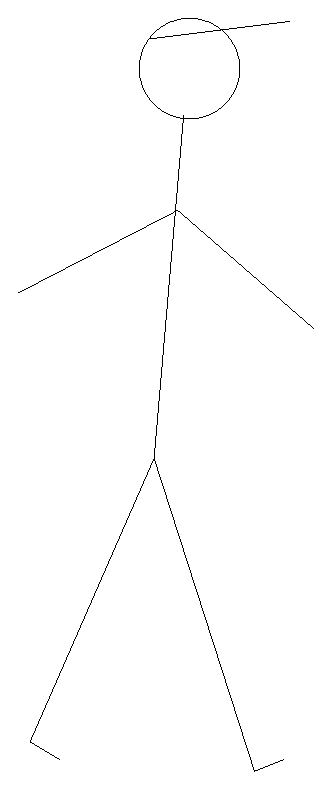
\includegraphics[width=w, height=h]{figura.eps} 
...
\end{document}
\end{verbatim} 

Los par{\'a}metros \verb|width| y \verb|height| son opcionales y puede
omitirse uno para que el sistema escale de acuerdo al par{\'a}metro dado.
Es posible variar la escala completa de la figura o rotarla usando
comandos disponibles en \verb+graphicx+.

\vspace{.3cm}
{\small
\begin{minipage}[t]{5cm}
Una figura aqu\'{\i}:

\begin{center}
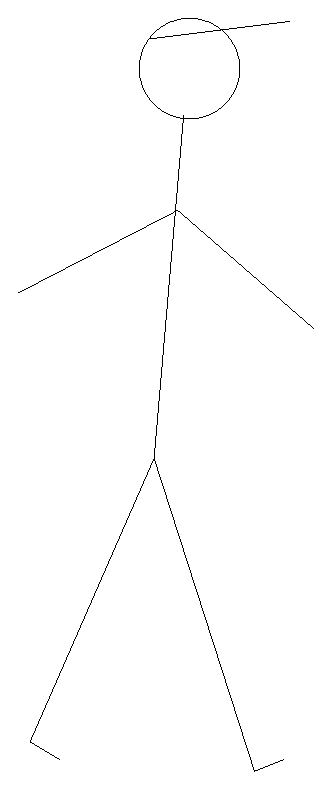
\includegraphics[height=3cm]{figura} % eps to pdf
\end{center}

puede hacer m\'as agradable el texto.
\end{minipage}
\hspace{1.5cm}
\begin{minipage}[t]{5cm}
\begin{verbatim}
Una figura aqu\'{\i}:

\begin{center}
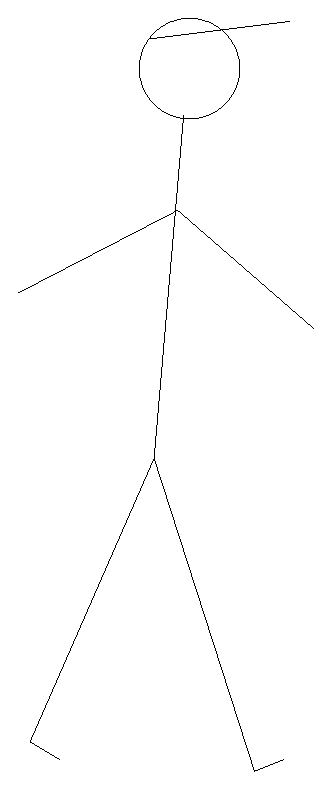
\includegraphics[height=3cm]{figura.eps} 
\end{center}

puede hacer m\'as agradable 
el texto.
\end{verbatim}
\end{minipage}
}
\vspace{.3cm}


En este ejemplo, indicamos s\'olo la altura de la figura
(3cm). El ancho fue determinado de modo que las proporciones de la
figura no fueran alteradas. Si no se especifica ni la altura ni el
ancho, la figura es insertada con su tama\~no natural. 

Observemos tambi\'en que pusimos la figura en un ambiente
\verb+center+. Esto no es necesario, pero normalmente uno desea que
las figuras est\'en centradas en el texto. 

\subsection{Ambiente {\tt figure}.}

Insertar una figura es una cosa. Integrarla dentro del texto es
otra. Para ello est\'a el ambiente \verb+figure+, que permite:
(a) posicionar la figura autom\'aticamente en un lugar predeterminado o
especificado por el usuario; (b) numerar las figuras; y (c) agregar un
breve texto explicativo junto a la figura.

Coloquemos la misma figura de la secci\'on anterior dentro de un
ambiente \verb+figure+. El input:
\begin{verbatim}
\begin{figure}[h]
\begin{center}
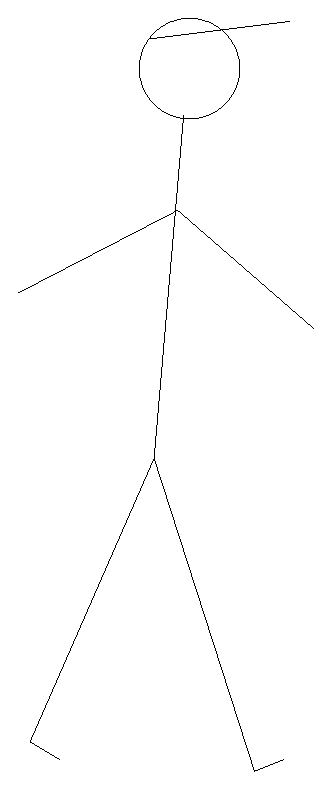
\includegraphics[height=3cm]{figura.eps} 
\end{center}
\caption{Un sujeto caminando.}
\label{caminando}
\end{figure}
\end{verbatim}
da como resultado:
\begin{figure}[h]
\begin{center}
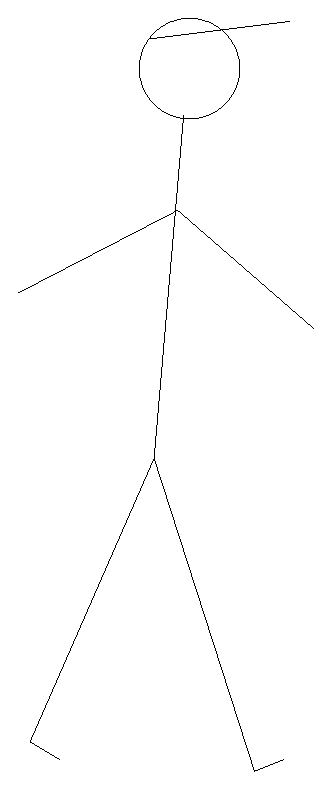
\includegraphics[height=3cm]{figura} % eps to pdf
\end{center}
\caption{Un sujeto caminando.}
\label{caminando}
\end{figure}

\verb+figure+ delimita lo que en \TeX\ se denomina un {\it objeto
  flotante}, es decir, un objeto cuya posici\'on no est\'a determinada
{\it a priori}, y se ajusta para obtener los mejores resultados
posibles. \TeX\ considera (de acuerdo con la tradici\'on), que la
mejor posici\'on para colocar una figura es al principio o al final de
la p\'agina. Adem\'as, lo ideal es que cada p\'agina tenga un cierto
n\'umero m\'aximo de figuras, que  ninguna figura
aparezca en el texto antes de que sea mencionada por primera
vez, y que, por supuesto, las figuras aparezcan en el orden en que son
mencionadas. \'Estas y otras condiciones determinan la posici\'on que un
objeto flotante tenga al final de la compilaci\'on. Uno puede forzar
la decisi\'on de \LaTeX\ con el argumento opcional de \verb+figure+:

\vspace{.3cm}
\begin{tabular}{lll}
\verb+t+&({\em top\/)} & extremo superior de la p\'agina \\
\verb+b+&({\em bottom\/}) & extremo inferior de la p\'agina\\
\verb+h+&({\em here\/}) & aqu\'{\i}, en el punto donde est\'a el
comando\\
\verb+p+&({\em page of floats\/}) & en una p\'agina separada al final
del texto
\end{tabular}
\vspace{.3cm}

El argumento adicional \verb+!+ suprime, para ese objeto flotante
espec\'{\i}fico, cualquier restricci\'on que exista sobre el n\'umero
m\'aximo de objetos flotantes en una p\'agina y el porcentaje de texto
m\'{\i}nimo que debe haber en una p\'agina.

Varios de estos argumentos se pueden colocar simult\'anemente, su
orden dictando la prioridad. Por ejemplo, 
\begin{verbatim}
\begin{figure}[htbp]
...
\end{figure}
\end{verbatim}
indica que la figura se debe colocar como primera prioridad aqu\'{\i}
mismo; si ello no es posible, al comienzo de p\'agina (\'esta o la
siguiente, dependiendo de los detalles de la compilaci\'on), y
as\'{\i} sucesivamente.

Adem\'as, \verb+figure+ numera autom\'aticamente la figura, colocando
el texto ``Figura $N$:'', y \verb+\caption+ permite colocar una
leyenda, centrada en el texto, 
a la figura. Puesto que la numeraci\'on es autom\'atica, las figuras
pueden ser referidas simb\'olicamente con \verb+\label+ y \verb+\ref+
(secci\'on \ref{referencias}). Para que la referencia sea correcta,
\verb+\label+ debe estar dentro del argumento de \verb+\caption+, o
despu\'es, como aparece en el ejemplo de la Figura \ref{caminando}
(\verb+\ref{caminando}+!).

Finalmente, notemos que la figura debi\'o ser centrada
expl\'{\i}citamente con \verb+center+. \verb+figure+ no hace nada
m\'as que tratar la figura como un objeto flotante, proporcionar
numeraci\'on y leyenda. El resto es responsabilidad del autor.   


\section{Cartas.}

Para escribir cartas debemos emplear el estilo \verb+letter+ en vez
del que hemos utilizado hasta ahora, \verb+article+. 
Comandos especiales permiten escribir
una carta, poniendo en lugares adecuados la direcci{\'o}n del remitente,
la fecha, la firma, etc. 

A modo de ejemplo, consideremos el siguiente input:

\begin{verbatim}
\documentclass[12pt]{letter}

\usepackage[spanish]{babel}

\begin{document}

\address{Las Palmeras 3425\\
\~Nu\~noa, Santiago}
\date{9 de Julio de 1998}

\signature{Pedro P\'erez \\ Secretario}

\begin{letter}{Dr.\ Juan P\'erez \\ Las Palmeras 3425 \\ 
\~Nu\~noa, Santiago} 
\opening{Estimado Juan}

A\'un no tenemos novedades.

Parece incre\'{\i}ble, pero los recientes acontecimientos nos han superado,
a pesar de nuestros esfuerzos.  Esperamos que mejores tiempos nos
aguarden.

\closing{Saludos,}
\cc{Arturo Prat \\ Luis Barrios}

\end{letter}
\end{document}
\end{verbatim} 

El resultado se encuentra en la pr\'oxima p\'agina.

\newpage

\ifpdf
   \vspace*{-2.2cm}\hspace*{-2cm}
   \includegraphics[height=28cm]{carta_sola.pdf}
\fi

Observemos que el texto de la carta est{\'a} dentro de un ambiente
\verb+letter+, el cual tiene un argumento obligatorio, donde aparece
el destinatario de la carta (con su direcci{\'o}n 
opcionalmente). 


Los comandos disponibles son:

\vspace{.3cm}
\begin{tabular}{lp{9cm}}
\verb+\address{<direccion>}+ & \verb+<direccion>+ del
remitente. \\[.3cm]
\verb+\signature{<firma>}+ & \verb+<firma>+ del remitente. \\[.3cm]
\verb+\opening{<apertura>}+ & F{\'o}rmula de \verb+<apertura>+.
\\[.3cm] 
\verb+\closing{<despedida>}+ & F{\'o}rmula de \verb+<despedida>+.
\\[.3cm] 
\verb+\cc{<copias>}+ & Receptores de \verb+<copias>+ (si los hubiera).
\end{tabular}
\vspace{.3cm}


Uno puede hacer m{\'a}s de una carta con distintos
ambientes \verb+letter+ en un mismo archivo. Cada una tomar{\'a} el
mismo remitente y firma dados por \verb+\address+ y
\verb+\signature+. Si deseamos que \verb+\address+ o
\verb+\signature+ valgan s{\'o}lo para una carta particular, basta
poner dichos comandos entre el \verb+\begin{letter}+ y el
\verb+\opening+ correspondiente.

Por ejemplo, la siguiente estructura:

\begin{verbatim}
\documentclass[12pt]{letter}
\begin{document}
\address{<direccion remitente>}
\date{<fecha>}
\signature{<firma>}

\begin{letter}{<destinatario 1>}
\opening<apertura 1>
...
\end{letter}

\begin{letter}{<destinatario 2>}
\address{<direccion remitente 2>}
\signature{<firma 2>}
\opening<apertura 2>
...
\end{letter}

\begin{letter}{<destinatario 3>}
\opening<apertura 3>
...
\end{letter}
\end{document}
\end{verbatim}
dar\'a origen a tres cartas con la misma direcci\'on de remitente y
firma, salvo la segunda. 

En todos estos comandos, l{\'\i}neas sucesivas son indicadas con
\verb+\\+. 

%\newpage

%\section{\bibtex}

%\bibtex\ no es una extensi\'on a \LaTeX, sino un programa
%independiente. Por ello, no se utiliza incluyendo en el pre\'ambulo
%una l\'{\i}nea de la forma \verb+\usepackage+, sino que corriendo un
%programa adicional. 

\section{\LaTeX\ y el formato {\tt pdf}.}

Junto con PostScript, otro formato ampliamente difundido
para la transmisi\'on de archivos, especialmente a trav\'es de
Internet, es el formato \verb+pdf+ (Portable Document Format). Para
generar un archivo \verb+pdf+ con \LaTeX\ es necesario compilarlo con
\verb+pdflatex+. As\'{\i}, \verb+pdflatex <archivo>+ generar\'a un
archivo \verb+<archivo>.pdf+ en vez del \verb+<archivo>.dvi+ generado
por el compilador usual. 

Si nuestro documento tiene figuras, s\'olo es posible incluirlas en el
documento si est\'an tambi\'en en formato \verb+pdf+. Por tanto, si
tenemos un documento con figuras en PostScript, debemos introducir dos
modificaciones antes de compilar con \verb+pdflatex+:

\begin{enumerate}[a)]
\item Cambiar el argumento de \verb+\includegraphics+ (secci\'on
  \ref{figuras}) de \verb+<archivo_figura>.eps+\linebreak a
  \verb+<archivo_figura>.pdf+.
\item Convertir las figuras PostScript a \verb+pdf+ (con
  \verb+epstopdf+, por ejemplo). Si tenemos una figura en el archivo
  \verb+<archivo_figura>.eps+, entonces 
\verb+epstopdf <archivo_figura>.eps+ genera el archivo correspondiente
\verb+<archivo_figura>.pdf+.
\end{enumerate}

Observar que el mismo paquete \verb+graphicx+ descrito en la secci\'on
\ref{figuras} para incluir figuras\linebreak \mbox{PostScript} permite, sin
modificaciones, incluir figuras en \verb+pdf+.

\section{Modificando  \LaTeX.}

Esta secci\'on se puede considerar ``avanzada''. Normalmente uno se
puede sentir satisfecho con el desempe\~no de \LaTeX, y no es
necesaria mayor intervenci\'on. A veces, dependiendo de la
aplicaci\'on y del autor, nos gustar\'{\i}a modificar el
comportamiento default. Una alternativa es definir nuevos comandos que
sean \'utiles para nosotros. Si esos nuevos comandos son abundantes, o
queremos reutilizarlos frecuentemente en otros documentos, lo
conveniente es considerar crear un nuevo paquete o incluso una nueva
clase. Examinaremos a continuaci\'on los elementos b\'asicos de estas
modificaciones. 

\subsection{Definici\'on de nuevos comandos.}

\subsubsection{El comando {\tt \bslash newcommand}}

Un nuevo comando se crea con:
\begin{verbatim}
\newcommand{<comando>}{<accion>}
\end{verbatim}

El caso m\'as sencillo es cuando una estructura se repite
frecuentemente en nuestro documento. Por ejemplo, digamos que un
sujeto llamado Crist\'obal no quiere escribir su nombre cada vez que
aparece en su documento:

\vspace{.3cm}
{\small
\begin{minipage}[t]{5cm}
\newcommand{\nombre}{Crist\'obal}
Mi nombre es \nombre. S\'{\i}, como oyes, \nombre. \nombre\ Loyola. 
\end{minipage}
\hspace{1.5cm}
\begin{minipage}[t]{5cm}
\begin{verbatim}
\newcommand{\nombre}{Crist\'obal}
...
\begin{document}
...
Mi nombre es \nombre. S\'{\i}, como oyes, 
\nombre. \nombre\ Loyola. 
\end{verbatim}
\end{minipage}
}
\vspace{.3cm}

Un \verb+\newcommand+ puede aparecer en cualquier parte del
documento, pero lo mejor es que est\'e en el pre\'ambulo, de modo que
sea evidente qu\'e nuevos comandos est\'an disponibles en el presente
documento. Observemos adem\'as que la definici\'on de un comando puede
contener otros comandos (en este caso, \verb+\'+). Finalmente, notamos
que ha sido necesario agregar un espacio expl\'{\i}cito con \verb+\ ,+
al escribir ``Crist\'obal Loyola'': recordemos que un comando comienza
con un backslash y termina con el primer car\'acter que no es
letra. Por tanto, \verb+\nombre Loyola+ ignora el espacio al final de
\verb+\nombre+, y el output ser\'{\i}a ``Crist\'obalLoyola''. 

Tambi\'en es posible definir comandos que funcionen en modo matem\'atico:

\vspace{.3cm}
{\small
\begin{minipage}[t]{5cm}
\newcommand{\vel}{\dot x}

Sea $\vel$ la velocidad, de modo que $\vel(t)> 0$ si $t<0$. 
\end{minipage}
\hspace{1.5cm}
\begin{minipage}[t]{5cm}
\begin{verbatim}
\newcommand{\vel}{\dot x}

Sea $\vel$ la velocidad, de modo que 
$ \vel(t)> 0$ si $t<0$. 
\end{verbatim}
\end{minipage}
}
\vspace{.3cm}

Como \verb+\vel+ contiene un comando matem\'atico (\verb+\dot+),
\verb+\vel+ s\'olo puede aparecer en modo matem\'atico.

Podemos tambi\'en incluir la apertura de modo matem\'atico en la
definici\'on de \verb+\vel+:\linebreak\verb+\newcommand{\vel}{$\dot x$}+. De
este modo, \verb+\vel+ (no \verb+$\vel$+) 
da como output directamente $\dot x$. Sin
embargo, esta soluci\'on no es \'optima, porque la siguiente
ocurrencia de \verb+\vel+ da un error. En efecto, si \verb+\vel+ =
\verb+$\dot x$+, entonces \verb+$ \vel(t)>0$+ = 
\verb+$ $\dot x$> 0$+. 
En tal caso, \LaTeX\ ve que un modo matem\'atico se ha abierto y
cerrado inmediatamente, conteniendo s\'olo un espacio entremedio, y
luego, {\em en modo texto}, viene el comando \verb+\dot+, que es
matem\'atico: \LaTeX\ acusa un error y la compilaci\'on se detiene. 

La soluci\'on a este problema es utilizar el comando
\verb+\ensuremath+, que asegura que haya modo matem\'atico, pero si ya
hay uno abierto, no intenta volverlo a abrir:

\vspace{.3cm}
{\small
\begin{minipage}[t]{5cm}
\newcommand{\vel}{\ensuremath{\dot x}}

Sea \vel\ la velocidad, de modo que $\vel(t)> 0$ si $t<0$. 
\end{minipage}
\hspace{1.5cm}
\begin{minipage}[t]{5cm}
\begin{verbatim}
\newcommand{\vel}{\ensuremath{\dot x}}

Sea \vel\ la velocidad, de modo que 
$ \vel(t)> 0$ si $t<0$. 
\end{verbatim}
\end{minipage}
}
\vspace{.3cm}

Un caso especial de comando matem\'atico es el de operadores tipo
logaritmo (ver Tabla \ref{logaritmo}). Si queremos definir una
traducci\'on al castellano de \verb+\sin+, debemos usar el comando
\verb+\DeclareMathOperator+ disponible via \verb+amsmath+:

\vspace{.3cm}
{\small
\begin{minipage}[t]{5cm}

Ahora podemos escribir en castellano, $\sen x$.
\end{minipage}
\hspace{1.5cm}
\begin{minipage}[t]{5cm}
\begin{verbatim}
\usepackage{amsmath}
\DeclareMathOperator{\sen}{sen}
...
Ahora podemos escribir en castellano, $\sen x$.
\end{verbatim}
\end{minipage}
}
\vspace{.3cm}

A diferencia de \verb+\newcommand+, \verb+\DeclareMathOperator+ s\'olo
puede aparecer en el pre\'ambulo del documento.


Un nuevo comando puede tambi\'en ser usado para ahorrar tiempo de
escritura, reemplazando comandos largos de \LaTeX:


\vspace{.3cm}
{\small
\begin{minipage}[t]{5cm}
\newcommand{\be}{\begin{enumerate}}
\newcommand{\ee}{\end{enumerate}}

\be
\item El primer caso.
\item Ahora el segundo.
\item Y el tercero.
\ee
\end{minipage}
\hspace{1.5cm}
\begin{minipage}[t]{5cm}
\begin{verbatim}
\newcommand{\be}{\begin{enumerate}}
\newcommand{\ee}{\end{enumerate}}

\be
\item El primer caso.
\item Ahora el segundo.
\item Y el tercero.
\ee
\end{verbatim}
\end{minipage}
}
\vspace{.3cm}

\subsubsection{Nuevos comandos con argumentos}

Podemos tambi\'en definir comandos que acepten argumentos. Si el
sujeto anterior, Crist\'obal,  desea escribir cualquier nombre precedido de
``Nombre:'' en it\'alica, entonces puede crear el siguiente comando:

\vspace{.3cm}
{\small
\begin{minipage}[t]{5cm}
\newcommand{\nombre}[1]{\textit{Nombre:} #1}
\nombre{Crist\'obal}

\nombre{Violeta}
\end{minipage}
\hspace{1.5cm}
\begin{minipage}[t]{5cm}
\begin{verbatim}
\newcommand{\nombre}[1]{\textit{Nombre:} #1}

\nombre{Crist\'obal}

\nombre{Violeta}
\end{verbatim}
\end{minipage}
}
\vspace{.3cm}

Observemos que \verb+\newcommand+ tiene un argumento opcional, que
indica el n\'umero de argumentos que el nuevo comando va a
aceptar. Esos argumentos se indican, dentro de la definici\'on del
comando, con \verb+#1+, \verb+#2+, etc. Por ejemplo, consideremos un 
comando que acepta dos argumentos:

\vspace{.3cm}
{\small
\begin{minipage}[t]{5cm}
\newcommand{\fn}[2]{f(#1,#2)}

$$ \fn{x}{y} + \fn{x_3}{y*} = 0 \ . $$
\end{minipage}
\hspace{1.5cm}
\begin{minipage}[t]{5cm}
\begin{verbatim}
\newcommand{\fn}[2]{f(#1,#2)}

$$ \fn{x}{y} + \fn{x_3}{y*} = 0 \ . $$
\end{verbatim}
\end{minipage}
}
\vspace{.3cm}

En los casos anteriores, todos los argumentos son obligatorios. \LaTeX\
permite definir comandos con un (s\'olo un) argumento opcional. Si el
comando acepta $n$ argumentos, el argumento opcional es
el \verb+#1+, y se debe indicar, en un segundo par\'entesis cuadrado,
su valor default. As\'{\i}, podemos modificar el comando \verb+\fn+
del ejemplo anterior para que el primer argumento sea opcional, con
valor default $x$:

\vspace{.3cm}
{\small
\begin{minipage}[t]{5cm}
\newcommand{\fn}[2][x]{f(#1,#2)}

$$ \fn{y} + \fn[x_3]{y*} = 0 \ . $$
\end{minipage}
\hspace{1.5cm}
\begin{minipage}[t]{5cm}
\begin{verbatim}
\newcommand{\fn}[2][x]{f(#1,#2)}

$$ \fn{y} + \fn[x_3]{y*} = 0 \ . $$
\end{verbatim}
\end{minipage}
}
\vspace{.3cm}

\subsubsection{Redefinici\'on de comandos}

Ocasionalmente no nos interesa definir un nuevo comando, sino
redefinir la acci\'on de un comando preexistente. Esto se hace con
\verb+\renewcommand+:

%%%%%%%%%%%%%%%%%%%%%%%%%%%%%%%%%%%%%%%%%%%%%%%%%%%%%%%%%%%%%%%%%%%%%%
%NOTA: El uso de \tt en vez de \verb en este ejemplo es intencional, 
%      porque no se ha discutido este comando
%%%%%%%%%%%%%%%%%%%%%%%%%%%%%%%%%%%%%%%%%%%%%%%%%%%%%%%%%%%%%%%%%%%%%%
\vspace{.3cm}
{\small
\begin{minipage}[t]{5cm}
La antigua versi\'on de {\tt ldots}: \ldots

\renewcommand{\ldots}{\textbullet \textbullet 
\textbullet}

La nueva versi\'on de {\tt ldots}: \ldots
\end{minipage}
\hspace{.5cm}
\begin{minipage}[t]{5cm}
\begin{verbatim}
La antigua versi\'on de  {\tt ldots}: \ldots

\renewcommand{\ldots}{\textbullet \textbullet 
\textbullet}

La nueva versi\'on de {\tt ldots}: \ldots
\end{verbatim}
\end{minipage}
}
\vspace{.3cm}


\subsubsection{P\'arrafos y cambios de l\'{\i}nea dentro de comandos}

En el segundo argumento de \verb+\newcommand+ o \verb+\renewcommand+
puede aparecer cualquier comando de \LaTeX, pero ocasionalmente la
aparici\'on de l\'{\i}neas en blanco (para forzar un cambio de
p\'arrafo) puede provocar problemas. Si ello ocurre, podemos usar
\verb+\par+, que hace exactamente lo mismo. Adem\'as, la definici\'on
del comando queda m\'as compacta:

\vspace{.3cm}
{\small
\begin{minipage}[t]{10cm}
\begin{verbatim}
\newcommand{\comandolargo}{\par Un nuevo comando que incluye un cambio de
  p\'arrafo, porque deseamos incluir bastante texto.\par \'Este es el
  nuevo p\'arrafo.\par}

Observemos en acci\'on el comando: \comandolargo Listo.
\end{verbatim}
\end{minipage}
}
\vspace{.3cm}

\noindent
da como resultado:

%NOTA: El efecto del comando tuvo que ser reproducido manualmente,
% debido a que dentro de minipage \parindent=0, y se ignora el
% \hspace* final por alguna razon
\hspace{3cm}\vspace{.3cm}
{\small
\begin{minipage}[t]{10cm}
\newcommand{\comandolargo}{\newline\hspace*{.5em}
 Un nuevo comando que incluye un cambio de
  p\'arrafo, porque deseamos incluir bastante
  texto.\newline\hspace*{.5em} 
\'Este es el
  nuevo p\'arrafo.\newline}

Observemos en acci\'on el comando: \comandolargo \hspace*{.8em}Listo.
\end{minipage}
}
\vspace{.6cm}

Un ejemplo m\'as \'util ocurre cuando queremos asegurar un cambio de
p\'arrafo, por ejemplo, para colocar un t\'{\i}tulo de secci\'on:

\vspace{.3cm}
{\small
\begin{minipage}[t]{5cm}
\newcommand{\seccion}[1]{\par\vspace{.5cm}{\bf Secci\'on: #1}\par\vspace{.5cm}}

Observemos en acci\'on el comando: \seccion{Ejemplo} Listo.
\end{minipage}
\hspace{1.5cm}
\begin{minipage}[t]{5cm}
\begin{verbatim}
\newcommand{\seccion}[1]{\par\vspace{.5cm}
{\bf Secci\'on: #1}\par\vspace{.5cm}}

Observemos en acci\'on el comando: 
\seccion{Ejemplo} Listo.
\end{verbatim}
\end{minipage}
}
\vspace{.3cm}

Adem\'as de las l\'{\i}neas en blanco, los cambios de l\'{\i}nea
pueden causar problemas dentro de la definici\'on de un nuevo
comando. El ejemplo anterior, con el comando \verb+\seccion+, es un
buen ejemplo: notemos que cuando se defini\'o, pusimos un cambio de
l\'{\i}nea despu\'es de \verb+\vspace{.5cm}+. Ese cambio de
l\'{\i}nea es interpretado (como todos los cambios de l\'{\i}nea) como
un espacio en blanco, y es posible que, bajo ciertas circunstancias,
ese espacio en blanco produzca un output no deseado. Para ello basta
utilizar sabiamente el car\'acter \verb+%+, que permite ignorar todo
el resto de la l\'{\i}nea, {\em incluyendo el cambio de
  l\'{\i}nea}. Ilustremos lo anterior con los siguientes tres
comandos, que subrayan (comando \verb+\underline+) una palabra, y 
difieren s\'olo en el uso de \verb+%+ para borrar
cambios de l\'{\i}nea:

\vspace{.3cm}
{\small
\begin{minipage}[t]{4cm}
\newcommand{\texto}{
Un texto de prueba
}
\newcommand{\textodos}{%
Un texto de prueba
}
\newcommand{\textotres}{%
Un texto de prueba%
}

Notar la diferencia entre: 

\underline{\texto},
\underline{\textodos}, 
y 
\underline{\textotres}.
\end{minipage}
\hspace{1.5cm}
\begin{minipage}[t]{5cm}
\begin{verbatim}
\newcommand{\texto}{
Un texto de prueba
}
\newcommand{\textodos}{%
Un texto de prueba
}
\newcommand{\textotres}{%
Un texto de prueba%
}

Notar la diferencia entre: 

\underline{\texto},
\underline{\textodos}, 
y 
\underline{\textotres}.
\end{verbatim}
\end{minipage}
}
\vspace{.3cm}

\verb+\texto+ conserva espacios en blanco antes y despu\'es del texto,
\verb+\textodos+ s\'olo el espacio en blanco despu\'es del texto, y
\verb+\textotres+ no tiene espacios en blanco alrededor del texto.


\subsubsection{Nuevos ambientes}

Nuevos ambientes en \LaTeX\ se definen con \verb+\newenvironment+:

\begin{verbatim}
\newenvironment{<ambiente>}{<comienzo ambiente>}{<final ambiente>}
\end{verbatim}
define un ambiente \verb+<ambiente>+, tal que \verb+\begin{ambiente}+
  ejecuta los comandos\linebreak \verb+<comienzo ambiente>+, y
  \verb+\end{ambiente}+ ejecuta los comandos \verb+<final ambiente>+. 

Definamos un ambiente que, al comenzar, cambia el font a it\'alica,
pone una l\'{\i}nea horizontal (\verb+\hrule+) y deja un espacio
vertical de .3cm, y que al terminar cambia de p\'arrafo, coloca
\verb+XXX+ en sans serif, deja un nuevo espacio vertical de .3cm, y
vuelve al font roman:


\vspace{.3cm}
{\small
\begin{minipage}[t]{10cm}
\begin{verbatim}
\newenvironment{na}{\it \hrule \vspace{.3cm}}{\par\sf XXX \vspace{.3cm}\rm}
\end{verbatim}
\end{minipage}
}
\vspace{.3cm}

Entonces, con

\vspace{.3cm}
{\small
\begin{minipage}[t]{10cm}
\begin{verbatim}
\begin{na}
  Hola a todos. Es un placer saludarlos en este d\'{\i}a tan especial.

Nunca esper\'e una recepci\'on tan calurosa.
\end{na}
\end{verbatim}
\end{minipage}
}
\vspace{.3cm}

\noindent
obtenemos:

{\small
\begin{center}
\begin{minipage}[t]{10cm}
\newenvironment{na}{\it \hrule \vspace{.3cm}}{\par\sf XXX \vspace{.3cm}\rm}
\begin{na}
  Hola a todos. Es un placer saludarlos en este d\'{\i}a tan especial.

Nunca esper\'e una recepci\'on tan calurosa.
\end{na}
\end{minipage}
\end{center}
}

Los nuevos ambientes tambi\'en pueden ser definidos de modo que
acepten argumentos. Como con \verb+\newcommand+, basta agregar como
argumento opcional a \verb+\newenvironment+ un n\'umero que indique
cu\'antos argumentos se van a aceptar:

\begin{verbatim}
\newenvironment{<ambiente>}[n]{<comienzo ambiente>}{<final ambiente>}
\end{verbatim}
Dentro de \verb+<comienzo ambiente>+, se alude a cada argumento como
\verb+#1+, \verb+#2+, etc. Los argumentos no pueden ser usados en los
comandos de cierre del ambiente (\verb+<final ambiente>+). Por
ejemplo, modifiquemos el ambiente \verb+na+ anterior, de modo que en
vez de colocar una l\'{\i}nea horizontal al comienzo, coloque lo que
le indiquemos en el argumento:

{\small
\begin{verbatim}
\newenvironment{na}[1]{\it #1 \vspace{.3cm}}{\par\sf XXX\hrule\vspace{.3cm}\rm}
\end{verbatim}
}

Ahora us\'emoslo dos veces, cada una con un argumento distinto:

\vspace{.3cm}
{\small
\begin{minipage}[t]{5cm}
\newenvironment{na}[1]{\it #1 \vspace{.3cm}}{\par\sf XXX\hrule\vspace{.3cm}\rm}
El mismo ejemplo anterior, ahora es

\begin{na}{\hrule}
  Hola a todos\ldots%. Es un placer saludarlos en este d\'{\i}a tan especial.
%
%Nunca esper\'e una recepci\'on tan calurosa.
\end{na}

Pero podemos ahora cambiar el comienzo:

\begin{na}{\it XXX}
  Hola a todos\ldots%. Es un placer saludarlos en este d\'{\i}a tan especial.
%
%Nunca esper\'e una recepci\'on tan calurosa.
\end{na}
\end{minipage}
\hspace{1.5cm}
\begin{minipage}[t]{5cm}
\begin{verbatim}
El mismo ejemplo anterior, ahora es

\begin{na}{\hrule}
  Hola a todos...
\end{na}

Pero podemos ahora cambiar el comienzo:

\begin{na}{\it XXX}
  Hola a todos...
\end{na}
\end{verbatim}
\end{minipage}
}
\vspace{.3cm}


\subsection{Creaci\'on de nuevos paquetes y clases}

Si la cantidad de nuevos comandos y/o ambientes que necesitamos en
nuestro documento es suficientemente grande, debemos considerar crear un nuevo
paquete o una nueva clase. Para ello hay que tener clara la diferencia
entre uno y otro. En general, se puede decir que si nuestros comandos
involucran alterar la apariencia general del documento, entonces
corresponde crear una nueva clase (\verb+.cls+). 
Si, por el contrario, deseamos que
nuestros comandos funcionen en un amplio rango de circunstancias, para
diversas apariencias del documento, entonces lo adecuado es un paquete
(\verb+.sty+).

Consideremos por ejemplo la experiencia de los autores de estos
apuntes. Para crear estos apuntes necesitamos b\'asicamente la clase
\verb+book+, con ciertas modificaciones: m\'argenes m\'as peque\~nos,
inclusi\'on autom\'atica de los paquetes \verb+amsmath+, \verb+babel+
y \verb+graphicx+, entre otros, y definici\'on de ciertos ambientes
espec\'{\i}ficos. Todo ello afecta la apariencia
de este documento, cambi\'andola de manera apreciable, pero a la vez
de un modo que en general no deseamos en otro tipo de documento. 
Por ello lo hemos compilado
usando una clase adecuada, llamada \verb+mfm2.cls+. 

Por otro lado, uno de los autores ha necesitado escribir muchas
tareas, pruebas y controles de ayudant\'{\i}a en su vida, y se ha
convencido de que su trabajo es m\'as f\'acil creando una clase
\verb+tarea.cls+, que sirve para esos tres prop\'ositos, definiendo
comandos que le permiten especificar f\'acilmente la fecha de entrega
de la tarea, o el tiempo disponible para una prueba, los nombres del
profesor y el ayudante, etc., una serie de comandos espec\'{\i}ficos
para sus necesidades. 

Sin embargo, tanto en este documento que usa \verb+mfm2.cls+, como
en las tareas y pruebas que usan \verb+tarea.cls+, se utilizan algunos
comandos matem\'aticos que no vienen con \LaTeX, pero que son
recurrentes, como \verb+\sen+ (la funci\'on seno en castellano),
\verb+\modulo+ (el m\'odulo de un vector),
 o \verb+\TLaplace+ (la transformada de Laplace).  Para que estos
 comandos est\'en disponibles en cualquier tipo de documento,
 necesitamos reunirlos en un paquete, en este caso
 \verb+addmath.sty+. De este modo, \verb+mfm2.cls+,
 \verb+tarea.cls+ o cualquier otra clase 
pueden llamar a este paquete y utilizar sus comandos. 

\subsubsection{Estructura b\'asica.}

La estructura b\'asica de un paquete o una clase es: 
\begin{enumerate}[a)]
\item Identificaci\'on: Informaci\'on general (nombre del
  paquete, fecha de creaci\'on, etc.). (Obligatoria.)
\item Declaraciones preliminares: Opcionales, dependiendo del paquete
  o clase en cuesti\'on. 
\item Opciones: Comandos relacionados con el manejo de las opciones
  con las cuales el paquete o clase pueden ser invocados. (Opcional.)
\item M\'as declaraciones: Aqu\'{\i} van los comandos que constituyen
  el cuerpo de la clase o paquete. (Obligatoria: si no hay ninguna
  declaraci\'on, el paquete o clase no hace nada, naturalmente.)
\end{enumerate}

La identificaci\'on est\'a consituida por las siguientes dos
l\'{\i}neas, que deben ir al comienzo del archivo:
\begin{verbatim}
\NeedsTeXFormat{LaTeX2e}
\ProvidesPackage{<paquete>}[<fecha> <otra informacion>]
\end{verbatim}

La primera l\'{\i}nea indica a \LaTeX\ que \'este es un archivo para
\LaTeXe. La segunda l\'{\i}nea especifica que se trata de un paquete,
indicando el nombre del mismo (es decir, el nombre del archivo sin
extensi\'on) y, opcionalmente, la fecha (en formato 
\verb+YYYY/MM/DD+) y otra informaci\'on relevante. Por ejemplo,
nuestro paquete \verb+addmath.sty+ comienza con las l\'{\i}neas:
\begin{verbatim}
\NeedsTeXFormat{LaTeX2e}
\ProvidesPackage{addmath}[1998/09/30 Macros matematicos adicionales (VM)]
\end{verbatim}

Si lo que estamos definiendo es una clase, usamos el comando
\verb+\ProvidesClass+. Para nuestra clase \verb+mfm2.cls+: 
\begin{verbatim}
\NeedsTeXFormat{LaTeX2e}
\ProvidesClass{mfm2}[2002/03/25 Estilo para apuntes MFM II (VM)]
\end{verbatim}

A continuaci\'on de la identificaci\'on vienen los comandos que
se desean incorporar a trav\'es de este paquete o clase. 

Como hemos dicho, \verb+addmath.sty+ contiene muchos nuevos comandos
matem\'aticos que consideramos necesario definir mientras
escrib\'{\i}amos estos apuntes. Veamos los contenidos de una versi\'on
simplificada de dicho paquete:
\begin{verbatim}
\NeedsTeXFormat{LaTeX2e}
\ProvidesPackage{addmath}[1998/09/30 Macros matematicos adicionales (VM)]

\newcommand{\prodInt}[2]{\ensuremath \left(\, #1\, |\, #2\, \right ) }
\newcommand{\promedio}[1]{\langle #1 \rangle}
\newcommand{\intii}{\int_{-\infty}^{\infty}}
\newcommand{\grados}{\ensuremath{^\circ}}
\newcommand{\Hipergeometrica}[4]{{}_2F_1\left (#1, #2, #3\, ; #4\right )}
...
\end{verbatim}

De este modo, incluyendo en nuestro documento el paquete con
\verb+\usepackage{addmath}+, varios nuevos comandos est\'an
disponibles:

$$
\begin{array}{lcl}
 \prodInt{x}{y}&&\mbox{\tt \bslash prodInt\{x\}\{y\}}  \\[.2cm]
 \promedio{x} &&\mbox{\tt \bslash promedio\{x\}}   \\[.2cm]
\displaystyle \intii dz\, f(z)&&\mbox{\tt \bslash intii dz\bslash, f(z)} \\[.2cm]
\angle\, ABC = 90\grados && \mbox{\tt \bslash angle\bslash, 
ABC = 90\bslash grados}\\[.2cm]
\Hipergeometrica{a}{b}{c}{d} &&\mbox{\tt \bslash Hipergeometrica\{a\}\{b\}\{c\}\{d\}} 
\end{array}
$$

\subsubsection{Incluyendo otros paquetes y clases}

Los comandos \verb+\RequirePackage+ y \verb+\LoadClass+ permiten
cargar un paquete o una clase, respectivamente.\footnote{Estos
  comandos s\'olo se pueden usar en un archivo {\tt .sty} o {\tt
    .cls} Para documentos normales, la manera de cargar un paquete es
  {\tt \bslash usepackage}, y para cargar una clase es {\tt \bslash
    documentclass}.}. Esto es de gran utilidad, pues permite construir
un nuevo paquete o clase aprovechando la funcionalidad de otros ya
existentes. 

As\'{\i}, nuestro paquete \verb+addmath.sty+ define bastantes
comandos, pero nos gustar\'{\i}a definir varios m\'as que s\'olo
pueden ser creados con las herramientas de \amslatex/. Cargamos
entonces en \verb+addmath.sty+ el paquete \verb+amsmath+ y otros
relacionados, y estamos en condiciones de crear m\'as comandos:

\begin{verbatim}
\NeedsTeXFormat{LaTeX2e}
\ProvidesPackage{addmath}[1998/09/30 Macros matematicos adicionales (VM)]

\RequirePackage{amsmath}
\RequirePackage{amssymb}
\RequirePackage{euscript}
...
\newcommand{\norma}[1]{\ensuremath \left\lVert\, #1 \,\right\rVert}
\newcommand{\intC}{{\sideset{^*}{}\int}} 
\DeclareMathOperator{\senh}{senh}
...
\end{verbatim}
Por ejemplo:

$$
\begin{array}{lcl}
 \norma{x}&&  \text{\tt \bslash norma\{x\}} \\[.2cm]
\intC dz \, f(z)&&\text{\tt \bslash intC dz \bslash, f(z)}  \\[.2cm]
\senh (2y) && \text{\tt \bslash senh (2y)}   
\end{array}
$$

La posibilidad de basar un archivo \verb+.sty+ o \verb+.cls+ en otro
es
 particularmente importante para una clase, ya que
 contiene una gran cantidad de comandos y definiciones
necesarias para compilar el documento exitosamente. Sin embargo, un
usuario normal, aun cuando desee definir una nueva clase, estar\'a
interesado en modificar s\'olo parte del comportamiento. Con
\verb+\LoadClass+, dicho usuario puede cargar la clase sobre la cual
se desea basar, y luego introducir las modificaciones necesarias,
facilitando enormemente la tarea.

Por ejemplo, al preparar este documento fue claro desde el comienzo
que se necesitaba esencialmente la clase \verb+book+, ya que
ser\'{\i}a un texto muy extenso, pero tambi\'en era claro que se
requer\'{\i}an ciertas modificaciones. Entonces, en nuestra clase
\verb+mfm2.cls+ lo primero que hacemos es cargar la clase \verb+book+,
m\'as algunos paquetes necesarios (incluyendo nuestro \verb+addmath+), 
y luego procedemos a modificar o a\~nadir comandos:

\begin{verbatim}
\NeedsTeXFormat{LaTeX2e}
\ProvidesClass{mfm2}[2002/03/25 Estilo para apuntes MFM II (VM)]

\LoadClass[12pt]{book}

\RequirePackage[spanish]{babel}
\RequirePackage{enumerate}
\RequirePackage{addmath}
\end{verbatim}

En un archivo \verb+.sty+ o un \verb+.cls+ se pueden cargar varios
paquetes con \verb+\RequirePackage+. \verb+\LoadClass+, en cambio,
s\'olo puede aparecer en un \verb+.cls+, y s\'olo es posible usarlo
una vez (ya que normalmente clases distintas son incompatibles entre
s\'{\i}). 

\subsubsection{Manejo de opciones}

En el \'ultimo ejemplo anterior, la clase \verb+mfm2+ carga la clase
\verb+book+ con la opci\'on \verb+12pt+. Esto significa que si nuestro
documento comienza con \verb+\documentclass{mfm2}+, ser\'a compilado
de acuerdo a la clase \verb+book+, en 12 puntos. No es posible cambiar
esto desde nuestro documento. Ser\'{\i}a mejor que pudi\'eramos
especificar el tama\~no de letra fuera de la clase, de modo que
\verb+\documentclass{mfm2}+ d\'e un documento en 10 puntos, y
\verb+\documentclass[12pt]{mfm2}+ uno en 12 puntos. Para lograr esto
hay que poder pasar opciones desde la clase \verb+mfm2+ a
\verb+book+. 

El modo m\'as simple de hacerlo es con
\verb+\LoadClassWithOptions+. Si \verb+mfm2.cls+ ha sido llamada con
opciones \verb+<opcion1>,<opcion2>, etc.+, entonces \verb+book+ ser\'a
llamada con las mismas opciones. Por tanto, basta modificar en
\verb+mfm2.cls+ la l\'{\i}nea \verb+\LoadClass[12pt]{book}+ por:
\begin{verbatim}
\LoadClassWithOptions{book}
\end{verbatim}


\verb+\RequirePackageWithOptions+ es el comando an\'alogo para
paquetes. Si una clase o un paquete llaman a un paquete
\verb+<paquete_base>+  y desean
pasarle todas las opciones con las cuales han sido invocados, basta
indicarlo con:
\begin{verbatim}
\RequirePackageWithOptions{<paquete_base>}
\end{verbatim}

El ejemplo anterior puede ser suficiente en muchas ocasiones, pero en
general uno podr\'{\i}a llamar a nuestra nueva clase, \verb+mfm2+, con
opciones que no tienen nada que ver con \verb+book+. Por ejemplo,
podr\'{\i}amos llamarla con opciones \verb+spanish,12pt+. En tal caso,
deber\'{\i}a pasarle \verb+spanish+ a babel, y \verb+12pt+ a
book. M\'as a\'un, podr\'{\i}amos necesitar definir una {\em nueva\/}
opci\'on, que no existe en ninguna de las clases o paquetes cargados
por \verb+book+, para modificar el comportamiento de \verb+mfm2.cls+
de cierta manera espec\'{\i}fica no prevista. Estas dos tareas,
discriminar entre opciones antes de pasarla a alg\'un paquete
determinado, y crear nuevas opciones, constituyen un manejo m\'as
avanzado de opciones. A continuaci\'on revisaremos un ejemplo
combinado de ambas tareas, extraido de la clase con la cual compilamos
este texto, \verb+mfm2.cls+.

La idea es poder llamar a \verb+mfm2+ con una opci\'on adicional
\verb+keys+, que permita agregar al \verb+dvi+ informaci\'on sobre las
etiquetas (dadas con \verb+\label+) de ecuaciones, figuras, etc., que
aparezcan en el documento (veremos la utilidad y un ejemplo de esto
 m\'as adelante). Lo primero es {\em declarar\/} una nueva opci\'on,
 con:
\begin{verbatim}
\DeclareOption{<opcion>}{<comando>}
\end{verbatim}
\verb+<opcion>+ es el nombre de la nueva opci\'on a declarar, y
\verb+<comando>+ es la serie de comandos que se ejecutan cuando dicha
opci\'on es especificada. 

As\'{\i}, nuestro archivo \verb+mfm2.cls+ debe ser modificado:
\begin{verbatim}
\NeedsTeXFormat{LaTeX2e}
\ProvidesClass{mfm2}[2002/03/25 Estilo para apuntes MFM II (VM)]
...
\DeclareOption{keys}{...}
...
\ProcessOptions\relax
...
\end{verbatim}

Observamos que despu\'es de declarar la o las opciones (en este caso
\verb+keys+), hay que {\em procesarlas}, con
\verb+\ProcessOptions+.\footnote{{\tt \bslash relax} es un comando de
    \TeX\ que, esencialmente, no hace nada, ni siquiera introduce un
    espacio en blanco, y es \'util incluirlo en puntos cr\'{\i}ticos
    de un documento, como en este ejemplo.}} 

Las l\'{\i}neas anteriores permiten que \verb+\documentclass{mfm2}+ y
\verb+\documentclass[keys]{mfm2}+ sean ambas v\'alidas, ejecut\'andose
o no ciertos comandos dependiendo de la forma utilizada. 

Si ahora queremos que \verb+\documentclass[keys,12pt]{mfm2}+ sea una
l\'{\i}nea v\'alida, debemos procesar \verb+keys+ dentro de
\verb+mfm2.cls+, y pasarle a \verb+book.cls+ las opciones
restantes. El siguiente es el c\'odigo definitivo:
\begin{verbatim}
\NeedsTeXFormat{LaTeX2e}
\ProvidesClass{mfm2}[2002/03/25 Estilo para apuntes MFM II (VM)]
\newif\ifkeys\keysfalse
\DeclareOption{keys}{\keystrue}
\DeclareOption*{\PassOptionsToClass{\CurrentOption}{book}}
\ProcessOptions\relax
\LoadClass{book}

\RequirePackage[spanish]{babel}
\RequirePackage{amsmath}
\RequirePackage{theorem}
\RequirePackage{epsfig}
\RequirePackage{ifthen}
\RequirePackage{enumerate}
\RequirePackage{addmath}
\ifkeys\RequirePackage[notref,notcite]{showkeys}\fi

<nuevos comandos de la clase mfm2.cls>
\end{verbatim}

Sin entrar en demasiados detalles, digamos que la opci\'on \verb+keys+
tiene el efecto de hacer que una cierta variable l\'ogica
\verb+\ifkeys+, sea verdadera (cuarta l\'{\i}nea del c\'odigo). La
siguiente l\'{\i}nea (\verb+\DeclareOption*...+) hace que todas las
opciones que no han sido procesadas (\verb+12pt+, por ejemplo)
se pasen a la clase \verb+book+. A continuaci\'on se procesan las
opciones con \verb+\ProcessOptions+, y finalmente se carga la clase
\verb+book+. 

Las l\'{\i}neas siguientes cargan todos los paquetes necesarios, y
finalmente se encuentran todos los nuevos comandos y definiciones
que queremos incluir en \verb+mfm2.cls+. 

Observemos que la forma particular en que se carga el paquete
\verb+showkeys+. \'Esa es precisamente la funci\'on de la opci\'on
\verb+keys+ que definimos: \verb+showkeys.sty+ se carga con ciertas
opciones s\'olo si se da la opci\'on \verb+keys+. 

?`Cu\'al es su
efecto? Consideremos el siguiente texto de ejemplo, en que \verb+mfm2+
ha sido llamada sin la opci\'on \verb+keys+:
\begin{verbatim}
\documentclass[12pt]{mfm2}              
\begin{document}
La opci\'on \verb+keys+ resulta muy \'util cuando tengo objetos numerados
autom\'aticamente, como una ecuaci\'on:
\begin{equation}
  \label{newton}
  \vec F = m \vec a \ . 
\end{equation}
y luego quiero referirme a ella: Ec.\  \eqref{newton}.
\end{verbatim}

En el primer caso, se ha compilado sin la opci\'on \verb+keys+, y en
el segundo con ella. El efecto es que, si se usa un \verb+\label+ en
cualquier parte del documento, aparece en el margen derecho una caja
con el nombre de dicha etiqueta (en este caso, \verb+newton+). 
Esto es \'util para cualquier tipo de
documentos, pero lo es especialmente en textos como
 estos apuntes, muy extensos y con
abundantes referencias. En tal caso, tener un modo visual, r\'apido,
de saber los nombres de las ecuaciones sin tener que revisar
trabajosamente el archivo fuente es una gran ayuda. As\'{\i},
versiones preliminares pueden ser compiladas con la opci\'on
\verb+keys+, y la versi\'on final sin ella, para no confesar al lector
nuestra mala memoria o nuestra comodidad.


\newpage


\ifpdf
 \vspace*{-2.2cm}\hspace*{-4cm}
 \includegraphics[height=28cm]{keys_example.pdf}
\fi

\section{Errores y advertencias.}

\subsection{Errores.}

Un mensaje de error t{\'\i}pico tiene la forma:\label{itemie}
\begin{verbatim}
LaTeX error. See LaTeX manual for explanation.
             Type H <return> for immediate help.
! Environment itemie undefined.
\@latexerr ...or immediate help.}\errmessage {#1}
                                                 \endgroup
l.140 \begin{itemie}

?  
\end{verbatim}


La primera l{\'\i}nea nos comunica que \LaTeX\ ha encontrado un
error. A veces los errores tienen que ver con  procesos m{\'a}s
internos, y son encontrados por \TeX. Esta l{\'\i}nea nos informa
qui{\'e}n encontr{\'o} el error. 

La tercera l{\'\i}nea comienza con un signo de exclamaci{\'o}n. {\'E}ste
es el indicador del error. Nos dice de qu{\'e} error se trata.

Las dos l{\'\i}neas siguientes describen el error en t{\'e}rminos de
comandos de bajo nivel.

La l{\'\i}nea 6 nos dice d{\'o}nde ocurri{\'o} el error: la l{\'\i}nea
140 en este caso. Adem{\'a}s nos informa del texto conflictivo:
\verb+\begin{itemie}+.
  
  En realidad, el mensaje nos indica d{\'o}nde \LaTeX\ advirti{\'o} el error
  por primera vez, que no es necesariamente el punto donde el error se
  cometi{\'o}. Pero la gran mayor{\'\i}a de las veces la indicaci{\'o}n es
  precisa. De hecho, es f{\'a}cil darse cuenta, con la tercera l{\'\i}nea\\
  (\verb+Environment itemie undefined+)\\ y la sexta
  (\verb+\begin{itemie}+) que el error consisti{\'o} en escribir
    \verb+itemie+ en vez de \verb+itemize+. La informaci{\'o}n de \LaTeX\ 
    es clara en este caso y nos dice correctamente qu{\'e} ocurri{\'o} y
    d{\'o}nde.

Luego viene un \verb+?+. \LaTeX\ est{\'a} esperando una respuesta de
nosotros. Tenemos varias alternativas. Comentaremos s{\'o}lo cuatro,
t{\'\i}picamente usadas:

\begin{list}{(\alph{enumi})}{\usecounter{enumi}%
\renewcommand{\theenumi}{(\alph{enumi})}}
\item \verb+h <Enter>+

Solicitamos ayuda. \TeX\ nos explica brevemente en qu{\'e} cree {\'e}l
que consiste el error y/o nos da alguna recomendaci{\'o}n.

\item \verb+x <Enter>+

Abortamos la compilaci{\'o}n. Deberemos volver al editor y corregir el
texto. Es la opci{\'o}n m{\'a}s t\'{\i}pica cuando uno tiene ya cierta
experiencia, pues el mensaje basta para reconocer el error.

\item \verb+<Enter>+
\label{Enter}

Ignoramos el error y continuamos la compilaci{\'o}n. \TeX\ hace lo que
puede. En algunos casos esto no tiene consecuencias
graves y podremos llegar hasta el final del archivo sin mayores
problemas. En otros casos, ignorar el error puede provocar que
ulteriores comandos ---perfectamente v{\'a}lidos en principio--- no
sean reconocidos y, as\'{\i}, acumular muchos errores m{\'a}s. Podemos
continuar con \verb+<Enter>+ sucesivos hasta llegar al final de la
compilaci{\'o}n. 

\item \verb+q <Enter>+
\label{q}

La acci{\'o}n descrita en el punto anterior puede llegar a ser tediosa o
infinita. \verb+q+ hace ingresar a \TeX\ en \verb+batchmode+, modo en
el cual la compilaci{\'o}n prosigue ignorando todos los errores hasta
el final del archivo, sin enviar mensajes a pantalla y por ende sin
que debamos darle infinitos \verb+<Enter>+. 

\end{list}

Las opciones \ref{Enter} y \ref{q} son
{\'u}tiles cuando no entendemos los mensajes de error. Como \TeX\ seguir{\'a}
compilando haciendo lo mejor posible, al mirar el \verb+dvi+ puede
que veamos m{\'a}s claramente d{\'o}nde comenzaron a ir mal las cosas y,
por tanto, por qu{\'e}.

\vspace{.3cm}
Como dijimos, \LaTeX\ indica exactamente d{\'o}nde encontr{\'o} el error,
de modo que hemos de ponerle atenci{\'o}n. Por ejemplo, si 
tenemos en nuestro documento la l\'{\i}nea:
\begin{verbatim}
... un error inesperado\fotnote{En cualquier punto.} 
puede decidir...
\end{verbatim}
generar\'{\i}a el mensaje de error:
\begin{verbatim}
! Undefined control sequence.

l.249 ...un error inesperado\fotnote
                                    {En cualquier punto.}
?
\end{verbatim}

En la l\'{\i}nea de localizaci{\'o}n, \LaTeX\ ha cortado el texto
justo despu{\'e}s del comando inexistente. \LaTeX\ no s{\'o}lo indica la
l\'{\i}nea en la cual detect{\'o} el error, sino el punto de ella donde
ello ocurri{\'o}. (En realidad, hizo lo mismo ---cortar la l\'{\i}nea
para hacer resaltar el problema--- en el caso expuesto en la
p{\'a}g.\ \pageref{itemie},  pero ello ocurri{\'o} en medio de comandos
de bajo nivel, as\'{\i} que no era muy informativo de todos modos.)

\subsubsection{Errores m{\'a}s comunes.}
\label{comunes}

Los errores m{\'a}s comunes son:
\begin{list}{\alph{enumi})}{\usecounter{enumi}%
\renewcommand{\theenumi}{\alph{enumi})}}
\item Comando mal escrito.
\label{mal}
\item Par{\'e}ntesis cursivos no apareados.
\label{cursivos}
\item Uso de uno de los caracteres especiales \verb+#+, \verb+$+,
\verb+%+, \verb+&+, \verb+_+, \verb+{+, \verb+}+, \verb+~+, \verb+^+,
\verb+\+ como texto ordinario.
\label{especiales}
\item Modo matem{\'a}tico abierto de una manera y cerrado de otra, o no
cerrado. 
\label{endmath}
\item Ambiente abierto con \verb+\begin...+ y cerrado con un
\verb+\end...+ distinto.
\label{endgroup}
\item Uso de un comando matem{\'a}tico fuera de modo matem{\'a}tico.
\label{mathmode}
\item Ausencia de argumento en un comando que lo espera.
\label{argumento}
\item L\'{\i}nea en blanco en ambiente matem{\'a}tico.
\label{blank}
\end{list}

\subsubsection{Algunos mensajes de error.}

A continuaci{\'o}n, una peque{\~n}a lista de errores (de \LaTeX\ y \TeX)
en orden alfab{\'e}tico, y sus posibles causas.

\begin{list}{}{\setlength{\leftmargin}{0pt}}
\item \verb+*+

Falta \verb+\end{document}+. (Dar \verb+Ctrl-C+ o escribir
\verb+\end{document}+ para salir de la compilaci{\'o}n.)

\item \verb+! \begin{...} ended by \end{...}+

Error \ref{endgroup} de la Sec.\ \ref{comunes}. El nombre del
ambiente en \verb+\end{...}+ puede estar mal escrito, sobra un
\verb+\begin+ o falta un \verb+\end+. 

\item \verb+! Double superscript+ (o \verb+subscript+).

Una expresi{\'o}n como \verb+x^2^3+ o \verb+x_2_3+. Si se desea obtener
${x^2}^3$ (${x_2}_3$), escribir \verb+{x^2}^3+ (\verb+{x_2}_3+). 

\item \verb+! Environment ... undefined.+

\verb+\begin{...}+ con un argumento que corresponde a un ambiente no
definido. 

\item \verb+! Extra alignment tab has been changed.+

En un \verb+tabular+ o \verb+array+ sobra un \verb+&+, falta un
\verb+\\+, o falta una \verb+c+, \verb+l+ {\'o} \verb+r+ en el
argumento obligatorio.

\item \verb+! Misplaced alignment tab character &.+

Un \verb+&+ aparece fuera de un \verb+tabular+ o \verb+array+.

\item \verb+! Missing $ inserted.+

Errores \ref{especiales}, \ref{endmath}, \ref{mathmode}, \ref{blank}
de la Sec.\ \ref{comunes}.

\item \verb+! Missing {+ (o \verb+}+) \verb+inserted.+

Par{\'e}ntesis cursivos no apareados.

\item \verb+! Missing \begin{document}.+

Falta \verb+\begin{document}+ o hay algo incorrecto en el
pre{\'a}mbulo. 

\item \verb+! Missing number, treated as zero.+

Falta un n{\'u}mero donde \LaTeX\ lo espera: \verb+\hspace{}+,
\verb+\vspace cm+,\linebreak \verb+\setlength{\textwidth}{a}+, etc.

\item \verb+! Something's wrong -- perhaps a missing \item.+

Posiblemente la primera palabra despu{\'e}s de un
\verb+\begin{enumerate}+ o\linebreak \verb+\begin{itemize}+ no es \verb+\item+. 

\item \verb+! Undefined control sequence.+

Aparece una secuencia \verb+\<palabra>+, donde \verb+<palabra>+ no es
un comando.

\end{list}

\subsection{Advertencias.}
\label{advertencias}

La estructura de una advertencia de \LaTeX\ es:
\begin{verbatim}
LaTeX warning. <mensaje>.
\end{verbatim}

Algunos ejemplos:

\begin{list}{}{\setlength{\leftmargin}{0pt}}
\item \verb+Label `...' multiply defined.+

Dos \verb+\label+ tienen el mismo argumento.

\item \verb+Label(s) may have changed. Rerun to get cross-references right.+ 

Los n{\'u}meros impresos por \verb+\ref+ y \verb+\pageref+ pueden ser
incorrectos, pues los valores correspondientes cambiaron respecto al
contenido del \verb+aux+ generado en la compilaci{\'o}n anterior.

\item \verb+Reference `...' on page ... undefined.+

El argumento de un \verb+\ref+ o un \verb+\pageref+ no fue definido
por un \verb+\label+.

\end{list}

\TeX\ tambi{\'e}n env\'{\i}a advertencias. Se reconocen porque no
comienzan con \verb+TeX warning+. 

Algunos ejemplos.

\begin{list}{}{\setlength{\leftmargin}{0pt}}
\item \verb+Overfull \hbox ...+

\TeX\ no encontr{\'o} un buen lugar para cortar una l\'{\i}nea, y puso
m{\'a}s texto en ella que lo conveniente.

\item \verb+Overfull \vbox ...+

\TeX\ no encontr{\'o} un buen lugar para cortar una p{\'a}gina, y puso
m{\'a}s texto en ella que lo conveniente.

\item \verb+Underfull \hbox ...+

\TeX\ construy{\'o} una l\'{\i}nea con muy poco material, de modo que
el espacio entre palabras puede ser excesivo.

\item \verb+Underfull \vbox ...+

\TeX\ construy{\'o} una p{\'a}gina con muy poco material, de modo que los
espacios verticales (entre p{\'a}rrafos) pueden ser excesivos.
\end{list}


Las advertencias de \LaTeX\ siempre deben ser atendidas. Una
referencia doblemente definida, o no compilar por segunda vez cuando
\LaTeX\ lo sugiere, generar{\'a} un resultado incorrecto en el
\verb+dvi+. Una referencia no definida, por su parte, hace aparecer
un signo {\bf ??} en el texto final. Todos resultados no deseados, por
cierto. 

Las advertencias de \TeX\ son menos decisivas. Un overfull o
underfull puede redundar en que alguna palabra se salga del margen
derecho del texto, que el espaciado entre palabras en una l\'{\i}nea
sea excesivo, o que el espacio vertical entre p{\'a}rrafos sea
demasiado. Los est{\'a}ndares de calidad de \TeX\ son altos, y por eso
env\'{\i}a advertencias frecuentemente. Pero generalmente los
defectos en el resultado final son imperceptibles a simple vista, o
por lo menos no son suficientes para molestarnos realmente. A veces
s\'{\i}, por supuesto, y hay que estar atentos. Siempre conviene
revisar el texto y prestar atenci{\'o}n a estos detalles, aunque ello
s{\'o}lo tiene sentido al preparar la versi{\'o}n definitiva del
documento. 




% Local Variables: 
% TeX-master: "mfm"
% End: 
  % TeX 
%\part{Ecuaciones diferenciales ordinarias.}
\include{mfm0-06} %Ec dif de primer orden
\include{mfm0-07} %Ec dif de orden > 1
\include{mfm0-08} %Sistema Ec dif 
%\part{M{\'e}todos Num{\'e}ricos.}
\include{mfm0-09} %Preliminares 
\setcounter{chapter}{9}
\chapter[EDO: M{\'e}todos b{\'a}sicos.]{Ecuaciones diferenciales ordinarias: M{\'e}todos b{\'a}sicos.}

\vspace{-1cm}
\hfill {\tiny versi{\'o}n preliminar 2.2-1 julio 2002\footnote{Este cap{\'\i}tulo est{\'a} basado en
    el segundo cap{\'\i}tulo del libro: {\em Numerical Methods for Physics,
      second edition} de Alejandro L. Garcia, editorial {\sc Prentice Hall}.} }

En este cap{\'\i}tulo resolveremos uno de los primeros problemas
considerados por un estudiante de f{\'\i}sica: el vuelo de un proyectil y,
en particular, el de una pelota de {\em baseball}. Sin la resistencia
del aire el problema es f{\'a}cil de resolver. Sin embargo, incluyendo un
arrastre realista, nosotros necesitamos calcular la soluci{\'o}n
num{\'e}ricamente. Para analizar este problema definiremos primero la
diferenciaci{\'o}n num{\'e}rica. De hecho antes de aprender F{\'\i}sica uno aprende
c{\'a}lculo as{\'\i} que no debemos sorprendernos si este es nuestro punto de
partida. En la segunda mitad del cap{\'\i}tulo nos acuparemos de otro viejo
conocido, el p{\'e}ndulo simple, pero sin la aproximaci{\'o}n a {\'a}ngulos
peque{\~n}os. Interesantemente, problemas oscilatorios, tales como el
p{\'e}ndulo, revelan una falla fatal en algunos de los m{\'e}todos num{\'e}ricos
para resolver ecuaciones diferenciales ordinarias.


\section{Movimiento de un proyectil.}
\label{c10-s1}

\subsection{Ecuaciones b{\'a}sicas.}

Consideremos el simple movimiento de un proyectil, digamos un pelota
de {\em baseball}. Para describir el movimiento nosotros debemos
calcular el vector posici{\'o}n $\vec r(t)$ y el vector velocidad
$\vec v(t)$ del proyectil. Las ecuaciones b{\'a}sicas de movimiento son
\begin{equation}
\label{c10-e2.1}
\frac{d\vec v}{dt}= \frac{1}{m} \vec F_a(\vec v\,) - g\hat y\ , \quad
\frac{d\vec r}{dt}= \vec v\ ,
\end{equation}
donde $m$ es la masa del proyectil. La fuerza debido a la resistencia
del aire es $\vec F_a(\vec v\,)$, la aceleraci{\'o}n gravitacional es $g$, e
$\hat y$ es un vector unitario en la direcci{\'o}n $y$. El movimiento es
bidimensional, tal que podemos ignorar la componente $z$ y trabajar en
el plano $xy$.

La resistencia del aire se incrementa con la velocidad del objeto, y
la forma precisa para $\vec F_a(\vec v\,)$ depende del flujo alrededor
del proyectil. Com{\'u}nmente, esta fuerza es aproximada por
\begin{equation}
\label{c10-e2.2}
\vec F_a(\vec v)= -\frac 12 C_d \rho A \modulo{v} \vec v\ ,
\end{equation}
donde $C_d$ es el coeficiente de arrastre, $\rho$ es la densidad del
aire, y $A$ es el {\'a}rea de la secci{\'o}n transversal del proyectil. El
coeficiente de arrastre es un par{\'a}metro adimensional que depende de la
geometr{\'\i}a del proyectil ---Mientras m{\'a}s aerodin{\'a}mico el objeto, el
coeficiente es menor.

Para una esfera suave de radio $R$ movi{\'e}ndose lentamente a trav{\'e}s del
fluido, el coeficiente de arrastre es dado por la Ley de Stokes,
\begin{equation}
\label{c10-e2.3}
C_d=\frac{12\nu}{Rv}=\frac{24}{\text{Re}}\ ,
\end{equation}
donde $\nu$ es la viscosidad del fluido ($\nu \approx 1.5\times10^{-5}$ [m$^2$/s]
para el aire) y $\text{Re}=2Rv/\nu$ es el adimensional {\em n{\'u}mero de
  Reynolds}. Para un objeto del tama{\~n}o de un pelota de baseball
movi{\'e}ndose a trav{\'e}s del aire, la ley de Stokes es v{\'a}lida s{\'o}lo si la
velocidad es menor que 0.2~[mm/s] ($\text{Re}\approx1$).

A velocidades altas (sobre 20~[cm/s], $\text{Re}>10^3$), la estela detr{\'a}s de
la esfera desarrolla v{\'o}rtices y el coeficiente de arrastre es
aproximadamente constante ($C_d\approx0.5$) para un amplio intervalo de
velocidades. Cuando el n{\'u}mero de Reynolds excede un valor cr{\'\i}tico, el
flujo en la estela llega a ser turbulento y el coeficiente de arrastre
cae dram{\'a}ticamente. Esta reducci{\'o}n ocurre porque la turbulencia rompe
la regi{\'o}n de bajas presiones en la estela detr{\'a}s de la
esfera\footnote{D.J. Tritton, {Physical Fluid Dynamics}, 2d ed.
  (Oxford: Clarendon Press, 1988).}. Para una esfera suave este n{\'u}mero
cr{\'\i}tico de Reynolds es aproximadamente $3\times10^5$. Para una pelota de
{\em baseball}, el coeficiente de arrastre es usualmente m{\'a}s peque{\~n}o
que el de una esfera suave, porque las costuras rompen el flujo
laminar precipitando el inicio de la turbulencia. Nosotros podemos
tomar $C_d=0.35$ como un valor promedio para el intervalo de
velocidades t{\'\i}picas de una pelota de {\em baseball}.

Notemos que la fuerza de arrastre, ecuaci{\'o}n (\ref{c10-e2.2}), var{\'\i}a
como el cuadrado de la magnitud de la velocidad ($\vec F_a\propto v^2$) y,
por supuesto, act{\'u}a en la direcci{\'o}n opuesta a la velocidad. La masa y
el di\'ametro de una pelota de {\em baseball} son 0.145~[kg] y 7.4~[cm].
Para una pelota de {\em baseball}, el arrastre y la fuerza
gravitacional son iguales en magnitud cuando $v\approx40$~[m/s].

Nosotros sabemos c{\'o}mo resolver las ecuaciones de movimiento si la
resistencia del aire es despreciable. La trayectoria es
\begin{equation}
\label{c10-e2.4}
\vec{r}(t)=\vec{r}_1+\vec{v}_1t- \frac 12 gt^2 \hat{y}\ ,
\end{equation}
donde $\vec{r}_1\equiv \vec{r}(0)$ y $\vec{v}_1\equiv \vec{v}(0)$ son la
posici{\'o}n y la velocidad inicial. Si el proyectil parte del origen y la
velocidad inicial forma un {\'a}ngulo $\theta$ con la horizontal, entonces
\begin{equation}
\label{c10-e2.5}
x_{\text{m{\'a}x}}=\frac{2v_1^2}{g} \sen \theta\cos\theta \ , \quad
y_{\text{m{\'a}x}} =\frac{v_1^2}{2g} \sen^2 \theta\ ,
\end{equation}
son el alcance horizontal y la altura m{\'a}xima. El tiempo de vuelo es
\begin{equation}
\label{c10-e2.6}
t_{fl}=\frac{2v_1}{g}\sen \theta\ .
\end{equation}

Nuevamente estas expresiones son v{\'a}lidas s{\'o}lo cuando no hay
resistencia con el aire. Es f{\'a}cil demostrar que el m{\'a}ximo alcance
horizontal se obtiene cuando la velocidad forma un {\'a}ngulo de
45$\grados$ con la horizontal. Deseamos mantener esta informaci{\'o}n en
mente cuando construyamos nuestra simulaci{\'o}n. Si se sabe la soluci{\'o}n
exacta para un caso especial, se debe comparar constantemente que el
programa trabaje bien para este caso.

\subsection{Derivada avanzada.}

Para resolver las ecuaciones de movimiento (\ref{c10-e2.1})
necesitamos un m{\'e}todo num{\'e}rico para evaluar la primera derivada. La
definici{\'o}n formal de la derivada es
\begin{equation}
\label{c10-e2.7}
f'(t)\equiv \lim_{\tau\to0}\frac{f(t+\tau)-f(t)}{\tau}\ ,
\end{equation}
donde $\tau$ es el incremento temporal o paso en el tiempo. Como ya vimos
en el cap{\'\i}tulo pasado esta ecuaci{\'o}n debe ser tratada con cuidado. La
figura \ref{c9-f2} ilustra que el uso de un valor extremadamente
peque{\~n}o para $\tau$ causa un gran error en el c{\'a}lculo de
$(f(t+\tau)-f(t))/\tau$. Espec{\'\i}ficamente, los errores de redondeo ocurren en
el c{\'a}lculo de $t+\tau$, en la evaluaci{\'o}n de la funci{\'o}n $f$ y en la
sustracci{\'o}n del numerador. Dado que $\tau$ no puede ser elegido
arbitrariamente peque{\~n}o, nosotros necesitamos estimar la diferencia
entre $f'(t)$ y $(f(t+\tau)-f(t))/\tau$ para un $\tau$ finito.

Para encontrar esta diferencia usaremos una expansi{\'o}n de Taylor. Como
f{\'\i}sicos usualmente vemos las series de Taylor expresadas como
\begin{equation}
\label{c10-e2.8}
f(t+\tau)=f(t)+\tau f'(t)+ \frac{\tau^2}{2}f''(t)+\cdots 
\end{equation}
donde los puntos suspensivos indican t{\'e}rminos de m{\'a}s alto orden que son
usualmente despreciados. Una alternativa, forma equivalente de la
serie de Taylor usada en an{\'a}lisis num{\'e}rico es
\begin{equation}
\label{c10-e2.9}
f(t+\tau)=f(t)+\tau f'(t)+ \frac{\tau^2}{2}f''(\zeta)\ ,
\end{equation}
donde $\zeta$ es un valor entre $t$ y $t+\tau$. No hemos botado ning{\'u}n
t{\'e}rmino, esta expansi{\'o}n tiene un n{\'u}mero finito de t{\'e}rminos. El teorema
de Taylor garantiza que existe {\em alg{\'u}n} valor $\zeta$ para el cual
(\ref{c10-e2.9}) es cierto, pero no sabemos cu{\'a}l valor es \'este.

La ecuaci{\'o}n previa puede ser reescrita
\begin{equation}
\label{c10-e2.10}
f'(t)=\frac{f(t+\tau)-f(t)}{\tau}-\frac 12 \tau f''(\zeta)\ ,
\end{equation} 
donde $t\leq \zeta\leq t +\tau$. Esta ecuaci{\'o}n es conocida como la f{\'o}rmula de la
{\em derivada derecha} o {\em derivada adelantada}. El {\'u}ltimo t{\'e}rmino
de la mano derecha es el {\em error de truncamiento}; este error es
introducido por cortar la serie de Taylor.

En otras palabras, si mantenemos el {\'u}ltimo t{\'e}rmino en
(\ref{c10-e2.10}), nuestra expresi{\'o}n para $f'(t)$ es exacta. Pero no
podemos evaluar este t{\'e}rmino porque no conocemos $\zeta$, todo lo que
conocemos es que $\zeta$ yace en alg{\'u}n lugar entre $t$ y $t+\tau$. As{\'\i}
despreciamos el t{\'e}rmino $f''(\zeta)$ (truncamos) y decimos que el error
que cometemos por despreciar este t{\'e}rmino es el error de truncamiento.
No hay que confundir {\'e}ste con el error de redondeo discutido
anteriormente. El error de redondeo depende del {\em hardware}, el
error de truncamiento depende de la aproximaci{\'o}n usada en el
algoritmo.  Algunas veces veremos la ecuaci{\'o}n (\ref{c10-e2.10})
escrita como
\begin{equation}
\label{c10-e2.11}
f'(t)=\frac{f(t+\tau)-f(t)}{\tau}+\DelOrdenD({\tau}) \ , 
\end{equation} 
donde el error de truncamiento es ahora especificado por su orden en
$\tau$, en este caso el error de truncamiento es lineal en $\tau$. En la
figura \ref{c9-f2} la fuente de error predominante en estimar $f'(x)$
como $[f(x+h)-f(x)]/h$  es el error de redondeo cuando $h<10^{-10}$ y
es el error de truncamiento cuando $h>10^{-10}$.

\subsection{M{\'e}todo de Euler.}

Las ecuaciones de movimiento que nosotros deseamos resolver
num{\'e}ricamente pueden ser escritas como:
\begin{equation}
\label{c10-e2.12}
\frac{d\vec v}{dt}=\vec{a}(\vec r, \vec v\,)\ , \quad \frac{d\vec
  r}{dt}= \vec{v}\ ,
\end{equation}
donde $\vec a$ es la aceleraci{\'o}n. Notemos que \'esta es la forma m{\'a}s
general de las ecuaciones. En el movimiento de proyectiles la
aceleraci{\'o}n es s{\'o}lo funci{\'o}n de $\vec v$ (debido al arrastre), en otros
problemas (e.g., \'orbitas de cometas) la aceleraci{\'o}n depender{\'a} de la
posici{\'o}n.

Usando la derivada adelantada (\ref{c10-e2.11}), nuestras ecuaciones
de movimiento son 
\begin{align}
\label{c10-e2.13}
\frac{\vec v (t+\tau)-\vec v (t)}{\tau} + \DelOrdenD(\tau) &=\vec a(\vec
r(t),\vec v(t)) \ ,\\
\label{c10-e2.14}
\frac{\vec r (t+\tau)-\vec r (t)}{\tau} + \DelOrdenD(\tau) &=\vec v(t) \ , 
\end{align}
o bien
\begin{align}
\label{c10-e2.15}
\vec v (t+\tau) &= \vec v (t) +\tau \vec a(\vec r(t),\vec v(t)) +
\DelOrdenD(\tau^2)\ ,\\
\label{c10-e2.16}
\vec r (t+\tau) &= \vec r (t) +\tau \vec v(t) + \DelOrdenD(\tau^2)\ .
\end{align}
Notemos que $\tau \DelOrdenD(\tau)= \DelOrdenD(\tau^2)$. Este esquema num{\'e}rico
es llamado el {\em m{\'e}todo de Euler}. Antes de discutir los m{\'e}ritos
relativos de este acercamiento, veamos c{\'o}mo ser{\'\i}a usado en la
pr{\'a}ctica.

Primero, introducimos la notaci{\'o}n
\begin{equation}
\label{c10-e2.17}
  f_n=f(t_n)\ , \quad t_n=(n-1)\tau\ , \quad n=1,2,\ldots
\end{equation}
tal que $f_1=f(t=0)$. Nuestras ecuaciones para el m{\'e}todo de Euler
(despreciando el t{\'e}rmino del error) ahora toman la forma
\begin{align}
\label{c10-e2.18}
\vec v_{n+1}  &= \vec v_n + \tau \vec a_n\ ,\\
\label{c10-e2.19}
\vec r_{n+1}  &= \vec r_n + \tau \vec v_n\ ,
\end{align}
donde $\vec a_n= \vec a(\vec r_n,\vec v_n)$. El c{\'a}lculo de la
trayectoria podr{\'\i}a proceder as{\'\i}:
\begin{enumerate}
\item Especifique las condiciones iniciales, $\vec r_1$ y $\vec v_1$.
\item Elija un paso de tiempo $\tau$.
\item Calcule la aceleraci{\'o}n dados los actuales $\vec r$ y $\vec v$.
\item Use las ecuaciones (\ref{c10-e2.18}) y (\ref{c10-e2.19}) para
  calcular los nuevos $\vec r$ y $\vec v$.
\item Vaya al paso 3 hasta que suficientes puntos de trayectoria hayan
  sido calculados.
\end{enumerate}
El m{\'e}todo calcula un conjunto de valores para $\vec r_n$ y $\vec v_n$
que nos da la trayectoria, al menos en un conjunto discreto de
valores. La figura \ref{c10-f1} ilustra el c{\'a}lculo de la trayectoria
para un {\'u}nico paso de tiempo.

\begin{figure}
\begin{center}
\includegraphics[width=7cm]{c10-f1}
\caption{Trayectoria de una part{\'\i}cula despu{\'e}s de un {\'u}nico paso de
  tiempo con el m{\'e}todo de Euler. S{\'o}lo para efectos ilustrativos $\tau$ es
  grande.}\label{c10-f1}
\end{center}
\end{figure}

\subsection{M{\'e}todos de Euler-Cromer y de Punto Medio.}

Una simple (y por ahora injustificada) modificaci{\'o}n del m{\'e}todo de
Euler es usar las siguientes ecuaciones:
\begin{align}
\label{c10-e2.20}
\vec v_{n+1}  &= \vec v_n + \tau \vec a_n\ ,\\
\label{c10-e2.21}
\vec r_{n+1}  &= \vec r_n + \tau \vec v_{n+1}\ .
\end{align}
Notemos el cambio sutil: La velocidad actualizada es usada en la
segunda ecuaci{\'o}n. Esta f{\'o}rmula es llamada {\em m{\'e}todo de
  Euler-Cromer}\footnote{A. Cromer, ``Stable solutions using the
  Euler approximation'', {\em Am. J. Phys.}, {\bf 49} 455-9 (1981).}.
El error de truncamiento es a{\'u}n del orden de $\DelOrdenD(\tau^2)$, no
parece que hemos ganado mucho. Interesantemente, veremos que esta
forma es marcadamente superior al m{\'e}todo de Euler en algunos casos. 

En el {\em m{\'e}todo del punto medio} usamos
\begin{align}
\label{c10-e2.22}
\vec v_{n+1}  &= \vec v_n + \tau \vec a_n\ ,\\
\label{c10-e2.23}
\vec r_{n+1}  &= \vec r_n + \tau \frac{\vec v_{n+1}+\vec v_n}2\ .
\end{align}
Notemos que hemos promediado las dos velocidades. Usando la ecuaci{\'o}n
para la velocidad en la ecuaci{\'o}n de la posici{\'o}n, vemos que
\begin{equation}
\label{c10-e2.24}
\vec r_{n+1} = \vec r_n + \tau \vec v_n + \frac 12  \vec a_n \tau^2\ ,
\end{equation}
lo cual realmente hace esto lucir atractivo. El error de truncamiento
es a{\'u}n del orden de $\tau^2$ en la ecuaci{\'o}n velocidad, pero para la
posici{\'o}n el error de truncamiento es ahora $\tau^3$. Realmente, para el
movimiento de proyectiles este m{\'e}todo trabaja mejor que los otros dos.
Infortunadamente, en otros sistemas f{\'\i}sicos este m{\'e}todo da resultados
pobres.

\subsection{Errores locales, errores globales y elecci{\'o}n del paso de
  tiempo.}

Para juzgar la precisi{\'o}n de estos m{\'e}todos necesitamos distinguir entre
errores de truncamiento locales y globales. Hasta ahora, el error de
truncamiento que hemos discutido ha sido el error local, el error
cometido en un {\'u}nico paso de tiempo. En un problema t{\'\i}pico nosotros
deseamos evaluar la trayectoria desde $t=0$ a $t=T$. El n{\'u}mero de
pasos de tiempo es $N_T=T/\tau$; notemos que si reducimos $\tau$, debemos
tomar m{\'a}s pasos. Si el error local es $\DelOrdenD(\tau^n)$, entonces
estimamos el error global como
\begin{equation}
\label{c10-e2.25}
\begin{split}
\text{error global}&\propto N_T \times (\text{error local})\\
&=N_T\DelOrdenD(\tau^n)=\frac
{T}{\tau}\DelOrdenD(\tau^n)=T\DelOrdenD(\tau^{n-1})\ .
\end{split}
\end{equation}
Por ejemplo, el m{\'e}todo de Euler tiene un error local de truncamiento
de $\DelOrdenD(\tau^2)$, pero un error global de truncamiento de
$\DelOrdenD(\tau)$. Por supuesto, este an{\'a}lisis nos da s{\'o}lo una
estimaci{\'o}n ya que no sabemos si los errores locales se acumular{\'a}n o se
cancelar{\'a}n ({\it i.e.} interferencia constructiva o destructiva). El
verdadero error global para un esquema num{\'e}rico es altamente
dependiente del problema que se est{\'a} estudiando.

Una pregunta que siempre aparece es ?`c{\'o}mo elegir el $\tau$? Tratemos de
responderla. Primero, supongamos que los errores de redondeo son
despreciables tal que s{\'o}lo debemos preocuparnos por los errores de
truncamiento. Desde (\ref{c10-e2.10}) y (\ref{c10-e2.16}), el error
local de truncamiento en el c{\'a}lculo de la posici{\'o}n usando el m{\'e}todo de
Euler es aproximadamente $\tau^2 r''=\tau^2a$. Usando s{\'o}lo estimaciones del
orden de magnitud, tomamos $a\approx10$~[m/s$^2$], el error en un solo paso
en la posici{\'o}n es de $10^{-1}$~[m], cuando $\tau=10^{-1}$~[s]. Si el
tiempo de vuelo $T\approx 10^0$~[s], entonces el error global es del orden
de metros. Si un error de esta magnitud es inaceptable entonces
debemos disminuir el paso en el tiempo. Finalmente usando un paso de
tiempo $10^{-1}$~[s] no introducir{\'\i}amos ning{\'u}n error significativo de
redondeo dada la magnitud de los otros par{\'a}metros del problema.

En el mundo real, a menudo no podemos hacer un an{\'a}lisis tan elegante
por una variedad de razones (ecuaciones complicadas, problemas con el
redondeo, flojera, etc.). Sin embargo, a menudo podemos usar la
intuici{\'o}n f{\'\i}sica. Resp{\'o}ndase usted mismo ``?`en qu{\'e} escala de tiempo
el movimiento es casi lineal?''. Por ejemplo, para la trayectoria
completa de una pelota de {\em baseball}, que es aproximadamente
parab{\'o}lica, el tiempo en el aire son unos pocos segundos, entonces el
movimiento es aproximadamente lineal sobre una escala de tiempo de
unos pocos cent{\'e}simos de segundo. Para revisar nuestra intuici{\'o}n,
nosotros podemos comparar los resultados obtenidos usando
$\tau=10^{-1}$~[s] y $\tau=10^{-2}$~[s] y, si ellos son suficientemente
cercanos, suponemos que todo est{\'a} bien. A veces automatizamos la
prueba de varios valores de $\tau$; el programa es entonces llamado {\em
  adaptativo} (construiremos un programa de este tipo m{\'a}s adelante).
Como con cualquier m{\'e}todo num{\'e}rico, la aplicaci{\'o}n ciega de esta
t{\'e}cnica es poco recomendada, aunque con s{\'o}lo un poco de cuidado {\'e}sta
puede ser usada exitosamente.

\begin{table}
\hrulefill
\begin{itemize}
\item Fijar la posici{\'o}n inicial $\vec r_1$ y la velocidad inicial
  $\vec v_1$ de la pelota de {\em baseball}.
\item Fijar los par{\'a}metros f{\'\i}sicos ($m$, $C_d$, etc.).
\item Iterar hasta que la bola golp\'ee en el piso o el m{\'a}ximo n{\'u}mero de
  pasos sea completado.
  \begin{itemize}
    \item Grabar posici{\'o}n (calculada y te{\'o}rica) para graficar.
    \item Calcular la aceleraci{\'o}n de la pelota de {\em baseball}.
    \item Calcular la nueva posici{\'o}n y velocidad, $\vec r_{n+1}$ y
      $\vec v_{n+1}$, Usando el m{\'e}todo de Euler, (\ref{c10-e2.18}) y
      (\ref{c10-e2.19}). 
    \item Si la pelota alcanza el suelo ($y<0$) para la iteraci{\'o}n.
\end{itemize}
\item Imprimir el alcance m{\'a}ximo y el tiempo de vuelo.
\item Graficar la trayectoria de la pelota de {\em baseball}.
\end{itemize}
\caption{Bosquejo del programa {\tt balle}, el cual calcula la trayectoria
  de una pelota de {\em baseball} usando el m{\'e}todo de Euler.}\label{c10-t1}
\hrulefill
\end{table}

\subsection{Programa de la pelota de {\em baseball}.}

La tabla \ref{c10-t1} bosqueja un simple programa, llamado
\verb|balle|, que usa el m{\'e}todo de Euler para calcular la trayectoria
de una pelota de {\em baseball}. Antes de correr el programa,
establezcamos algunos valores razonables para tomar como entradas. Una
velocidad inicial de $\modulo{\vec v_1}=$15~[m/s] nos da una pelota
que le han pegado d{\'e}bilmente. Partiendo del origen y despreciando la
resistencia del aire, el tiempo de vuelo es de 2.2~[s], y el alcance
horizontal es sobre los 23~[m] cuando el {\'a}ngulo inicial $\theta=45\grados$.
A continuaci{\'o}n, mostramos la salida a pantalla del programa
\verb|balle| en C++ cuando es corrido bajo estas condiciones.

\begin{figure}[!h]
\begin{center}
\includegraphics[angle =-90, width=10cm]{c10-f2}
\caption{Salida del programa {\tt balle} para una altura inicial de
  0~[m], una velocidad inicial de 15~[m/s], y un paso de tiempo
  $\tau=$0.1~[s]. No hay resistencia del aire. La l{\'\i}nea continua es la
  te{\'o}rica y los puntos son los calculados, la diferencia se debe a
  errores de truncamiento.}\label{c10-f2}
\end{center}
\end{figure}
\begin{verbatim}
jrogan@huelen:~/programas$ balle
Ingrese la altura inicial [m] : 0
Ingrese la velocidad inicial [m/s]: 15
Ingrese angulo inicial (grados): 45
Ingrese el paso en el tiempo, tau en [s]: 0.1
Tiempo de vuelo: 2.2
Alcance: 24.3952
\end{verbatim}%$ 
La salida en Octave debiera ser muy similar. 

La trayectoria calculada por el programa es mostrada en la figura
\ref{c10-f2}. Usando un paso de $\tau=0.1$~[s], el error en el alcance
horizontal es sobre un metro, como esper{\'a}bamos del error de
truncamiento. A velocidades bajas los resultados no son muy diferentes
si incluimos la resistencia con el aire, ya que $|\vec F_{a}(\vec
v_1)|/m\approx g/7$.

Ahora tratemos de batear un cuadrangular. Consideremos una velocidad
inicial grande $\modulo{v_1}=50$~[m/s]. Debido a la resistencia,
encontramos que el alcance es reducido a alrededor de 125~[m], menos
de la mitad de su maximo te{\'o}rico. La trayectoria es mostrada figura
\ref{c10-f3}, notemos c\'omo se aparta de la forma parab{\'o}lica.

En nuestras ecuaciones para el vuelo de una pelota de {\em baseball}
no hemos incluido todos los factores en el problema. El coeficiente de
arrastre no es constante sino m{\'a}s bien una complicada funci{\'o}n de la
velocidad. Adem{\'a}s, la rotaci{\'o}n de la pelota ayuda a levantar la pelota
(efecto Magnus).

\begin{figure}[!h]
\begin{center}
\includegraphics[angle =-90, width=10cm]{c10-f3}
\caption{Salida del programa {\tt balle} para una altura inicial de
  1~[m], una velocidad inicial de 50~[m/s], y un paso de tiempo
  $\tau=$0.1~[s]. Con resistencia del aire.}\label{c10-f3}
\end{center}
\end{figure}

\section{P{\'e}ndulo simple.}

\subsection{Ecuaciones b{\'a}sicas.}

El movimiento de los p{\'e}ndulos ha fascinado a f{\'\i}sicos desde que Galileo
fue hipnotizado por la l{\'a}mpara en la Catedral de Pisa. El problema es
tratado en los textos de mec{\'a}nica b{\'a}sica pero antes de apresurarnos a
calcular con el computador, revisemos algunos resultados b{\'a}sicos. Para
un p{\'e}ndulo simple es m{\'a}s conveniente describir la posici{\'o}n en t{\'e}rminos
del desplazamiento angular, $\theta(t)$. La ecuaci{\'o}n de movimiento es
\begin{equation}
\label{c10-e2.26}
\frac{d^2\theta}{dt^2}= - \frac{g}{L}\sen \theta\ ,
\end{equation}
donde $L$ es la longitud del brazo y $g$ es la aceleraci{\'o}n de
gravedad. En la aproximaci{\'o}n para {\'a}ngulo peque{\~n}o, $\sen \theta \approx \theta$, la
ecuaci{\'o}n (\ref{c10-e2.26}) se simplifica a
\begin{equation}
\label{c10-e2.27}
\frac{d^2\theta}{dt^2}= - \frac{g}{L}\theta\ .
\end{equation} 
Esta ecuaci{\'o}n diferencial ordinaria es f{\'a}cilmente resuelta para
obtener
\begin{equation}
\label{c10-e2.28}
\theta(t)=C_1\cos \left ( \frac{2\pi t}{T_s} + C_2 \right )\ ,
\end{equation}
donde las constantes $C_1$ y $C_2$ est{\'a}n determinadas por los valores
iniciales de $\theta$ y $\omega=d\theta/ dt$. El per{\'\i}odo para {\'a}ngulos peque{\~n}os,
$T_s$ es
\begin{equation}
\label{c10-e2.29}
T_s=2\pi\sqrt{\frac Lg}\ .
\end{equation}
Esta aproximaci{\'o}n es razonablemente buena para oscilaciones con
amplitudes menores o iguales a $20\grados$.

Sin la aproximaci{\'o}n para {\'a}ngulos peque{\~n}os, la ecuaci{\'o}n de movimiento
es m{\'a}s dif{\'\i}cil de resolver. Sin embargo, sabemos de la experiencia que
el movimiento es todav{\'\i}a peri{\'o}dico. En efecto, es posible obtener una
expresi{\'o}n para el per{\'\i}odo sin resolver expl{\'\i}citamente $\theta(t)$. La
energ{\'\i}a total es
\begin{equation}
\label{c10-e2.30}
E=\frac 12 m L^2\omega^2- mgL\cos \theta\ ,
\end{equation}
donde $m$ es la masa de la lenteja. La energ{\'\i}a total es conservada e
igual a $E=-mgL\cos \theta_m$, donde $\theta_m$ es el {\'a}ngulo m{\'a}ximo. De lo
anterior, tenemos 
\begin{equation}
\label{c10-e2.31}
\frac 12 m L^2\omega^2 -mgL\cos \theta = -mgL\cos \theta_m\ ,
\end{equation}
o
\begin{equation}
\label{c10-e2.32}
\omega^2 =\frac{2g}L \left ( \cos \theta - \cos \theta_m \right ) \ .
\end{equation}
Ya que $\omega=d\theta/dt$, 
\begin{equation}
\label{c10-e2.33}
dt=\frac{d\theta}{\sqrt{\dfrac {2g}L \left ( \cos \theta - \cos \theta_m \right
    )}}\ .
\end{equation} 
En un per{\'\i}odo el p{\'e}ndulo se balancea de $\theta=\theta_m$ a $\theta=-\theta_m$ y regresa a
$\theta=\theta_m$. As{\'\i}, en medio per{\'\i}odo el p{\'e}ndulo se balancea desde $\theta=\theta_m$ a
$\theta=-\theta_m$. Por {\'u}ltimo, por el mismo argumento, en un cuarto de per{\'\i}odo
el p{\'e}ndulo se balancea desde $\theta=\theta_m$ a $\theta=0$, as{\'\i} integrando ambos
lados de la ecuaci{\'o}n (\ref{c10-e2.33})
\begin{equation}
\label{c10-e2.34}
\frac{T}{4}=\sqrt{\frac L{2g} } \int_0^{\theta_m}\frac{d\theta}{\sqrt{\left ( \cos \theta - \cos \theta_m \right
    )}}\ .
\end{equation} 

Esta integral podr{\'\i}a ser reescrita en t{\'e}rminos de funciones especiales
usando la identidad $\cos 2\theta=1-2\sen^2 \theta$, tal que 
\begin{equation}
\label{c10-e2.35}
T=2\sqrt{\frac Lg } \int_0^{\theta_m}\frac{d\theta}{\sqrt{\left ( \sen^2
      \theta_m/2 -\sen^2 \theta/2\right  )}}\ .
\end{equation} 
Introduciendo $K(x)$, la integral el{\'\i}ptica completa de primera
especie,\footnote{I.S. Gradshteyn and I.M. Ryzhik, {\em Table of
    Integral, Series and Products} (New York: Academic Press, 1965)}
\begin{equation}
\label{c10-e2.36}
K(x)\equiv\int_0^{\pi/2} \frac{dz}{\sqrt{1-x^2\sen^2 z}}\ ,
\end{equation}
podr{\'\i}amos escribir el per{\'\i}odo como 
\begin{equation}
\label{c10-e2.37}
T=4\sqrt{\frac{L}{g}} K(\sen \theta_m/2 )\ ,
\end{equation}
usando el cambio de variable $\sen z= \sen( \theta/2)/ \sen(\theta_m/2)$. Para
valores peque{\~n}os de $\theta_m$, podr{\'\i}amos expandir $K(x)$ para obtener
\begin{equation}
\label{c10-e2.38}
T=2\pi \sqrt{\frac{L}{g} }\left ( 1 + \frac{1}{16}\,  \theta^2_m + \ldots \right
)\ .
\end{equation}
Note que el primer t{\'e}rmino es la aproximaci{\'o}n para {\'a}ngulo peque{\~n}o
(\ref{c10-e2.29}). 

\subsection{F{\'o}rmulas para la derivada centrada.}

Antes de programar el problema del p{\'e}ndulo miremos un par de otros
esquemas para calcular el movimiento de un objeto. El m{\'e}todo de Euler
est{\'a} basado en la formulaci{\'o}n de la derivada derecha para $df/dt$ dado
por (\ref{c10-e2.7}). Una definici{\'o}n equivalente para la derivada es 
\begin{equation}
\label{c10-e2.39}
f'(t)=\lim_{\tau\to0} \frac{f(t+\tau)-f(t-\tau)}{2\tau}\ .
\end{equation}
Esta f{\'o}rmula se dice centrada en $t$. Mientras esta f{\'o}rmula parece muy
similar a la ecuaci{\'o}n (\ref{c10-e2.7}), hay una gran diferencia cuando
$\tau$ es finito. Nuevamente, usando la expansi{\'o}n de Taylor,
\begin{align}
\label{c10-e2.40}
f(t+\tau)&=f(t)+\tau f'(t)+\frac 12 \tau^2 f''(t)+\frac 16 \tau^3 f^{(3)}(\zeta_+)\ ,\\
\label{c10-e2.41}
f(t-\tau)&=f(t)-\tau f'(t)+\frac 12 \tau^2 f''(t)-\frac 16 \tau^3 f^{(3)}(\zeta_-)\ ,
\end{align}
donde $f^{(3)}$ es la tercera derivada de $f(t)$ y $\zeta_{\pm}$ es un
valor ente $t$ y $t \pm\tau$. Restando las dos ecuaciones anteriores y
reordenando tenemos,
\begin{equation}
\label{c10-e2.42}
f'(t)=\frac{f(t+\tau)-f(t-\tau)}{2\tau}-\frac 16 \tau^2 f^{(3)}(\zeta)\ ,
\end{equation}
donde $t-\tau\leq \zeta\leq t+\tau$. Esta es la {\em aproximaci{\'o}n en la primera
  derivada centrada}. El punto clave es que el error de truncamiento
es ahora cuadr{\'a}tico en $\tau$, lo cual es un gran progreso sobre la
aproximaci{\'o}n de las derivadas adelantadas que tiene un error de
truncamiento $\DelOrdenD(\tau)$.

Usando las expansiones de Taylor para $f(t+\tau)$ y $f(t-\tau)$ podemos
construir una f{\'o}rmula centrada para la segunda derivada. La que tiene
la forma
\begin{equation}
\label{c10-e2.43}
f''(t)=\frac{f(t+\tau)+f(t-\tau)-2f(t)}{\tau^2}- \frac 1{12}\tau^2 f^{(4)}(\zeta)\ ,
\end{equation}
donde $t-\tau\leq\zeta\leq t+\tau$. De nuevo, el error de truncamiento es cuadr{\'a}tico
en $\tau$. La mejor manera de entender esta f{\'o}rmula es pensar que la
segunda derivada est{\'a} compuesta de una derivada derecha y de una
derivada izquierda, cada una con incrementos de $\tau/2$.

Usted podr{\'\i}a pensar que el pr{\'o}ximo paso ser{\'\i}a preparar f{\'o}rmulas m{\'a}s
complicadas que tengan errores de truncamiento a{\'u}n m{\'a}s peque{\~n}os,
quiz{\'a}s usando ambas $f(t\pm\tau)$ y $f(t\pm 2\tau)$. Aunque tales f{\'o}rmulas
existen y son ocasionalmente usadas, las ecuaciones (\ref{c10-e2.10}),
(\ref{c10-e2.42}) y (\ref{c10-e2.43}) sirven como el ``caballo de
trabajo'' para calcular las derivadas primera y segunda.

\subsection{M{\'e}todos del ``salto de la rana'' y de Verlet.}

Para el p{\'e}ndulo, las posiciones y velocidades generalizadas son $\theta$ y
$\omega$, pero para mantener la misma notaci{\'o}n anterior trabajaremos con $\vec
r$ y $\vec v$. Comenzaremos de las ecuaciones de movimiento escritas
como 
\begin{align}
\label{c10-e2.44}
\frac{d\vec v}{dt} &= \vec a(\vec r(t))\ ,\\
\label{c10-e2.45}
\frac{d\vec r}{dt} &= \vec v(t)\ .
\end{align}
Note que expl{\'\i}citamente escribimos la aceleraci{\'o}n dependiente
solamente de la posici{\'o}n. Discretizando la derivada temporal usando la
aproximaci{\'o}n de derivada centrada da,
\begin{equation}
\label{c10-e2.46}
\frac {\vec v(t+\tau)- \vec v(t-\tau)}{2\tau}+\DelOrdenD(\tau^2)=\vec a(\vec
r(t))\ ,
\end{equation}
para la ecuaci{\'o}n de la velocidad. Note que aunque los valores de
velocidad son evaluados en $t+\tau$ y $t-\tau$, la aceleraci{\'o}n es evaluada
en el tiempo $t$.

Por razones que pronto ser{\'a}n claras, la discretizaci{\'o}n de la ecuaci{\'o}n
de posici{\'o}n estar{\'a} centrada entre $t+2\tau$ y $t$, 
\begin{equation}
\label{c10-e2.47}
\frac{\vec r(t+2\tau)- \vec r(t)}{2\tau}+\DelOrdenD(\tau^2)=\vec v(t+\tau)\ .
\end{equation}
De nuevo usamos la notaci{\'o}n $f_n\equiv f(t=(n-1)\tau)$, en la cual la
ecuaci{\'o}n (\ref{c10-e2.47}) y (\ref{c10-e2.46}) son escritas como, 
\begin{align}
\label{c10-e2.48}
\frac {\vec v_{n+1}- \vec v_{n-1}}{2\tau}+\DelOrdenD(\tau^2)&=\vec a(\vec r_n)\ ,\\
\label{c10-e2.49}
\frac{\vec r_{n+2}- \vec r_n}{2\tau}+\DelOrdenD(\tau^2)&=\vec v_{n+1}\ .
\end{align}
Reordenando los t{\'e}rminos para obtener los valores futuros a la
izquierda, 
\begin{align}
\label{c10-e2.50}
\vec v_{n+1}&= \vec v_{n-1}+2\tau\vec a(\vec r_n)+ \DelOrdenD(\tau^3)\ ,\\
\label{c10-e2.51}
\vec r_{n+2} &=\vec r_n + 2\tau\vec v_{n+1}+\DelOrdenD(\tau^3)\ ,
\end{align}
el cual es el {\em m{\'e}todo del ``salto de la rana'' (leap frog)}.
Naturalmente, cuando el m{\'e}todo es usado en un programa, el t{\'e}rmino
$\DelOrdenD(\tau^3)$ no va y por lo tanto constituye el error de
truncamiento para el m{\'e}todo.

El nombre ``salto de la rana'' es usado ya que la soluci{\'o}n avanza en
pasos de $2\tau$, con la posici{\'o}n evaluada en valores impares ($\vec
r_1$, $\vec r_3$, $\vec r_5$, \ldots), mientras que la velocidad est{\'a}
calculada en los valores pares ($\vec v_2$, $\vec v_4$, $\vec v_6$,
\ldots). Este entrelazamiento es necesario ya que la aceleraci{\'o}n, la cual
es una funci{\'o}n de la posici{\'o}n, necesita ser evaluada en a tiempo, esto
es centrada entre la nueva velocidad y la antigua. Algunas veces el
esquema del ``salto de la rana'' es formulado como
\begin{align}
\label{c10-e2.52}
\vec v_{n+1/2}&= \vec v_{n-1/2}+\tau\vec a(\vec r_n)\ ,\\
\label{c10-e2.53}
\vec r_{n+1} &=\vec r_n + \tau\vec v_{n+1/2}\ ,
\end{align}
con $\vec v_{n\pm1/2}\equiv \vec v(t=(n-1\pm1/2)\tau)$. En esta forma, el
esquema es funcionalmente equivalente al m{\'e}todo de Euler-Cromer. 

Para el {\'u}ltimo esquema num{\'e}rico de este cap{\'\i}tulo tomaremos una
aproximaci{\'o}n diferente y empezaremos con,
\begin{align}
\label{c10-e2.54}
\frac{d\vec r}{dt}&=\vec v(t)\ ,\\
\label{c10-e2.55}
\frac{d^2\vec r}{dt^2}&=\vec a(\vec r)\ .
\end{align}
Usando las f{\'o}rmulas diferenciales centradas para la primera y segunda
derivada, tenemos 
\begin{align}
\label{c10-e2.56}
\frac{\vec r_{n+1}-\vec r_{n-1}}{2\tau}+ \DelOrdenD(\tau^2)&=\vec v_n\ ,\\
\label{c10-e2.57}
\frac{\vec r_{n+1}+\vec r_{n-1}-2\vec r_n}{\tau^2}+ \DelOrdenD(\tau^2)&=\vec a_n\ ,
\end{align}
donde $\vec a_n\equiv \vec a (\vec r_n)$. Reordenando t{\'e}rminos, 
\begin{align}
\label{c10-e2.58}
\vec v_n &= \frac{\vec r_{n+1}-\vec r_{n-1}}{2\tau}+ \DelOrdenD(\tau^2)\ ,\\[2mm]
\label{c10-e2.59}
\vec r_{n+1}&=2\vec r_{n}-\vec r_{n-1}+ \tau^2\vec a_n +\DelOrdenD(\tau^4)\ .
\end{align}

Estas ecuaciones, conocidas como el {\em m{\'e}todo de
  Verlet}\footnote{L.Verlet, ``Computer experiments on classical fluid
  I. Thermodynamical properties of Lennard-Jones molecules'', {\em
    Phys. Rev.} {\bf 159}, 98-103 (1967).}, podr{\'\i}an parecer extra{\~n}as a
primera vista, pero ellas son f{\'a}ciles de usar. Suponga que conocemos
$\vec r_0$ y $\vec r_1$; usando la ecuaci{\'o}n (\ref{c10-e2.59}),
obtenemos $\vec r_2$. Conociendo $\vec r_1$ y $\vec r_2$ podr{\'\i}amos
ahora calcular $\vec r_3$, luego usando la ecuaci{\'o}n (\ref{c10-e2.58})
obtenemos $\vec v_2$, y as{\'\i} sucesivamente.

Los m{\'e}todos del ``salto de la rana'' y de Verlet tienen la desventaja que
no son ``autoiniciados''. Usualmente tenemos las condiciones iniciales
$\vec r_1=\vec r(t=0)$ y $\vec v_1=\vec v(t=0)$, pero no $\vec v_0=
\vec v(t=-\tau)$ [necesitado por el ``salto de la rana'' en la ecuaci{\'o}n
(\ref{c10-e2.50})] o $\vec r_0=\vec r(t=-\tau)$ [necesitado por Verlet
en la ecuaci{\'o}n (\ref{c10-e2.59})]. Este es el precio que hay que pagar
para los esquemas centrados en el tiempo.

Para lograr que estos m{\'e}todos partan, tenemos una variedad de
opciones. El m{\'e}todo de Euler-Cromer, usando la ecuaci{\'o}n
(\ref{c10-e2.53}), toma $\vec v_{1/2}=\vec v_1$, lo cual es simple
pero no muy precisa. Una alternativa es usar otro esquema para lograr
que las cosas partan, por ejemplo, en el ``salto de la rana'' uno
podr{\'\i}a tomar un paso tipo Euler para atr{\'a}s, $\vec v_0=\vec v_1-\tau\vec
a_1$. Algunas precauciones deber{\'\i}an ser tomadas en este primer paso
para preservar la precisi{\'o}n del m{\'e}todo; usando
\begin{equation}
\label{c10-e2.60}
\vec r_0=\vec r_1-\tau \vec v_1 + \frac{\tau^2}{2} \, \vec a(\vec r_1)\ ,
\end{equation}
es una buena manera de comenzar el m{\'e}todo de Verlet.

Adem{\'a}s de su simplicidad, el m{\'e}todo del ``salto de la rana'' a menudo
tiene propiedades favorables ({\it e.g.} conservaci{\'o}n de la energ{\'\i}a)
cuando resuelve ciertos problemas. El m{\'e}todo de Verlet tiene muchas
ventajas. Primero, la ecuaci{\'o}n de posici{\'o}n tiene un error de
truncamiento menor que otros m{\'e}todos. Segundo, si la fuerza es
solamente una funci{\'o}n de la posici{\'o}n y si nos preocuparnos s{\'o}lo de la
trayectoria de la part{\'\i}cula y no de su velocidad (como en muchos
problemas de mec{\'a}nica celeste), podemos saltarnos completamente el
c{\'a}lculo de velocidad. El m{\'e}todo es popular para el c{\'a}lculo de las
trayectorias en sistemas con muchas part{\'\i}culas, por ejemplo, el
estudio de fluidos a nivel microsc{\'o}pico.

\begin{table}
\hrulefill
\begin{itemize}
\item Seleccionar el m{\'e}todo a usar: Euler o Verlet.
\item Fijar la posici{\'o}n inicial $\theta_1$ y la velocidad $\omega_1=0$ del p{\'e}ndulo.
\item Fijar los par{\'a}metros f{\'\i}sicos y otras variables.
\item Tomar un paso para atr{\'a}s para partir Verlet; ver ecuaci{\'o}n (\ref{c10-e2.60}).
\item Iterar sobre el n{\'u}mero deseado de pasos con el paso de tiempo y
  m{\'e}todo num{\'e}rico dado.
  \begin{itemize}
  \item Grabar {\'a}ngulo y tiempo para graficar.
  \item Calcular la nueva posici{\'o}n y velocidad usando el m{\'e}todo de
    Euler o de Verlet.
  \item Comprobar si el p{\'e}ndulo a pasado a trav{\'e}s de $\theta=0$; Si es
    as{\'\i} usar el tiempo transcurrido para estimar el per{\'\i}odo.
\end{itemize}
\item Estima el per{\'\i}odo de oscilaci{\'o}n, incluyendo barra de error.
\item Graficar las oscilaciones como $\theta$ versus $t$.
\end{itemize}
\caption{Bosquejo del programa {\tt pendulo}, el cual calcula el tiempo
  de evoluci{\'o}n de un p{\'e}ndulo simple usando el m{\'e}todo de Euler o Verlet.}\label{c10-t2}
\hrulefill
\end{table}

\subsection{Programa de p{\'e}ndulo simple.}

Las ecuaciones de movimiento para un p{\'e}ndulo simple son
\begin{equation}
\label{c10-e2.61}
\frac{d\omega}{dt}=\alpha(\theta)\, \quad \frac{d\theta}{dt}=\omega\ ,
\end{equation}
donde la aceleraci{\'o}n angular $\alpha(\theta)=-g \sen\theta /L$. El m{\'e}todo de Euler
para resolver estas ecuaciones diferenciales ordinarias es iterar las
ecuaciones: 
\begin{align}
\label{c10-e2.62}
\theta_{n+1}=\theta_n+\tau\omega_n\ ,\\
\label{c10-e2.63}
\omega_{n+1}=\omega_n+\tau\alpha_n\ .
\end{align}
Si estamos interesados solamente en el {\'a}ngulo y no la velocidad, el
m{\'e}todo de Verlet s{\'o}lo usa la ecuaci{\'o}n
\begin{equation}
\label{c10-e2.64}
\theta_{n+1}=2\theta_n-\theta_{n-1}+\tau^2\alpha_n\ .
\end{equation}

En vez de usar las unidades SI, usaremos las unidades adimensionales
naturales del problema. Hay solamente dos par{\'a}metros en el problema,
$g$ y $L$ y ellos siempre aparecen en la raz{\'o}n $g/L$. Fijando esta
raz{\'o}n a la unidad, el per{\'\i}odo para peque{\~n}as amplitudes $T_s=2\pi$. En
otras palabras, necesitamos s{\'o}lamente una unidad en el problema: una
escala de tiempo. Ajustamos nuestra unidad de tiempo tal que el
per{\'\i}odo de peque{\~n}as amplitudes sea $2\pi$.

La tabla \ref{c10-t2} presenta un bosquejo del programa \verb|pendulo|,
el cual calcula el movimiento de un p{\'e}ndulo simple usando o el m{\'e}todo
de Euler o el de Verlet. El programa estima el per{\'\i}odo por registrar
cuando el {\'a}ngulo cambia de signo; esto es verificar si $\theta_n$ y
$\theta_{n+1}$ tienen signos opuestos probando si $\theta_n*\theta_{n+1}<0$. Cada
cambio de signo da una estimaci{\'o}n para el per{\'\i}odo,
$\tilde{T}_k=2\tau(n_{k+1}-n_k)$, donde $n_k$ es el paso de tiempo en el
cual el $k$-{\'e}simo cambio de signo ocurre. El per{\'\i}odo estimado de cada
inversi{\'o}n de signo es registrado, y el valor medio calculado como
\begin{equation}
\label{c10-e2.65}
\left \langle \tilde{T}\right \rangle =\frac 1M\sum_{k=1}^M \tilde{T}_k\ ,
\end{equation}
donde $M$ es el n{\'u}mero de veces que $\tilde{T}$ es evaluado. La barra
de error para esta medici{\'o}n del per{\'\i}odo es estimada como $\sigma=s/M$,
donde
\begin{equation}
\label{c10-e2.66}
s=\sqrt{\frac{1}{M-1}\sum_{k=1}^M 
\left (\tilde{T}_k-\left \langle \tilde{T}\right \rangle\right )^2}\ ,
\end{equation}
es la desviaci{\'o}n estandar de la muestra $\tilde{T}$. Note que cuando
el n{\'u}mero de medidas se incrementa, la desviaci{\'o}n estandar de la
muestra tiende a una constante, mientras que la barra de error
estimado decrese.

Para comprobar el programa \verb|pendulo|, primero tratamos con {\'a}ngulos
iniciales peque{\~n}os, $\theta_m$, ya que conocemos el per{\'\i}odo $T\approx 2\pi$.
Tomando $\tau=0.1$ tendremos sobre 60 puntos por oscilaci{\'o}n; tomando 300
pasos deber{\'\i}amos tener como cinco oscilaciones. Para $\theta_m=10\grados$,
El m{\'e}todo de Euler calcula un per{\'\i}odo estimado de $\langle \tilde{T}\rangle=
6.375\pm0.025$ sobre un 1.5\% mayor que el esperado $T=2\pi(1.002)$ dado
por la ecuaci{\'o}n (\ref{c10-e2.38}). Nuestro error estimado para el
per{\'\i}odo es entorno a $\pm\tau$ en cada medida. Cinco oscilaciones son 9
medidas de $\tilde T$ , as{\'\i} que nuestro error estimado para el per{\'\i}odo
deber{\'\i}a ser $(\tau/2)/ \sqrt{9}\approx0.02$. Notemos que la estimaci{\'o}n est{\'a} en
buen acuerdo con los resultados obtenidos usando la desviaci{\'o}n
estandar.  Hasta aqu{\'\i} todo parece razonable.

\begin{figure}[!h]
\begin{center}
\includegraphics[angle =-90, width=10cm]{c10-f4}
\caption{Salida del programa {\tt pendulo} usando el m{\'e}todo de
  Euler. El {\'a}ngulo inicial es $\theta_m=10\grados$, el paso en el tiempo es
  $\tau=0.1$, y 300 iteraciones fueron calculadas.}\label{c10-f4}
\end{center}
\end{figure}

Infortunadamente si miramos el grafico \ref{c10-f3} nos muestra los
problemas del m{\'e}todo de Euler. La amplitud de oscilaci{\'o}n crece con el
tiempo. Ya que la energ{\'\i}a es proporcional al {\'a}ngulo m{\'a}ximo, esto
significa que la energ{\'\i}a total se incrementa en el tiempo. El error
global de truncamiento en el m{\'e}todo de Euler se acumula en este caso.
Para pasos de tiempos peque{\~n}os $\tau=0.05$ e incrementos en el n{\'u}mero de
pasos (600) podemos mejorar los resultados, ver figura \ref{c10-f4},
pero no eliminamos el error. El m{\'e}todo del punto medio tiene la misma
inestabilidad num{\'e}rica.

\begin{figure}[!h]
\begin{center}
\includegraphics[angle =-90, width=10cm]{c10-f5}
\caption{Salida del programa {\tt pendulo} usando el m{\'e}todo de
  Euler. El {\'a}ngulo inicial es $\theta_m=10\grados$, el paso en el tiempo es
  $\tau=0.05$ y 600 iteraciones fueron calculadas.}\label{c10-f5}
\end{center}
\end{figure}

\begin{figure}[!h]
\begin{center}
\includegraphics[angle =-90, width=10cm]{c10-f6}
\caption{Salida del programa {\tt pendulo} usando el m{\'e}todo de
  Verlet. El {\'a}ngulo inicial es $\theta_m=10\grados$, el paso en el tiempo es
  $\tau=0.1$ y 300 iteraciones fueron calculadas.}\label{c10-f6}
\end{center}
\end{figure}

Usando el m{\'e}todo de Verlet con $\theta_m=10\grados$, el paso en el tiempo
$\tau=0.1$ y 300 iteraciones obtenemos los resultados graficados en
\ref{c10-f5}. Estos resultados son mucho mejores; la amplitud de
oscilaci{\'o}n se mantiene cerca de los $10\grados$ y $\langle \tilde
T\rangle=6.275\pm0.037$. Afortunadamente el m{\'e}todo de Verlet, el del ``salto
de rana'' y el de Euler-Cromer no sufren de la inestabilidad num{\'e}rica
encontrada al usar el m{\'e}todo de Euler.

\begin{figure}[!h]
\begin{center}
\includegraphics[angle =-90, width=10cm]{c10-f7}
\caption{Salida del programa {\tt pendulo} usando el m{\'e}todo de
  Verlet. El {\'a}ngulo inicial es $\theta_m=170\grados$, el paso en el tiempo es
  $\tau=0.1$ y 300 iteraciones fueron calculadas.}\label{c10-f7}
\end{center}
\end{figure}

Para $\theta_m=90\grados$, la primera correcci{\'o}n para la aproximaci{\'o}n de
{\'a}ngulo peque{\~n}o, ecuaci{\'o}n (\ref{c10-e2.38}), da $T=7.252$. Usando el
m{\'e}todo de Verlet, el programa da un per{\'\i}odo estimado de
$\langle\tilde{T}\rangle=7.414\pm 0.014$, lo cual indica que (\ref{c10-e2.38}) es
una buena aproximaci{\'o}n (alrededor de un 2\% de error), a{\'u}n para {\'a}ngulos
grandes. Para el {\'a}ngulo muy grande de $\theta_m=170\grados$, vemos la
trayectoria en la figura \ref{c10-f6}. Notemos como la curva tiende a
aplanarse en los puntos de retorno. En este caso el per{\'\i}odo estimado
es $\langle\tilde{T}\rangle=15.3333+/-0.0667$, mientr{\'a}s que (\ref{c10-e2.38}) da
$T=9.740$, indicando que esta aproximaci{\'o}n para (\ref{c10-e2.37}) deja
de ser v{\'a}lida para este {\'a}ngulo tan grande.  


\section{Listado de los  programas.}

\subsection{\tt balle.cc}

\begin{verbatim}
#include "NumMeth.h"

main()
{
  const double Cd=0.35;
  const double rho=1.293;               // [kg/m^3]
  const double radio=0.037;                     // [m]
  double A= M_PI*radio*radio ;  
  double m=0.145;                               // [kg] 
  double g=9.8;                 // [m/s^2]
  double a = -Cd*rho*A/(2.0e0*m) ;

  double v0, theta0, tau;
  ofstream salida ("salida.txt") ;
  ofstream salidaT ("salidaT.txt") ;

  double x0, y0; 
  x0=0.0e0 ;
  cout << "Ingrese la altura inicial [m] : ";
  cin >> y0;
  cout << "Ingrese la velocidad inicial [m/s]: ";
  cin >> v0;
  cout <<"Ingrese angulo inicial (grados): ";
  cin >> theta0;

  int flagRA = 2 ;
  while (flagRA!=0 && flagRA !=1) {
    cout <<"Con resistencia del aire, Si= 1, No= 0: ";
    cin >> flagRA;
  }
  cout <<"Ingrese el paso en el tiempo, tau en [s]: "; 
  cin >> tau ;
  double vxn=v0*cos(M_PI*theta0/180.0) ;
  double vyn=v0*sin(M_PI*theta0/180.0) ;
  double xn=x0 ;
  double yn=y0 ;
  double tiempo = -tau;
  while( yn >= y0) {
    tiempo +=tau ;
    salidaT << x0+v0*cos(M_PI*theta0/180.0) *tiempo <<" " ;
    salidaT << y0+v0*sin(M_PI*theta0/180.0) *tiempo -g*tiempo*tiempo/2.0e0<< endl;
    salida << xn << " " << yn << endl;
    if(flagRA==0) a=0.0e0 ; 
    double v=sqrt(vxn*vxn+vyn*vyn) ;
    double axn= a*v*vxn ;
    double ayn= a*v*vyn -g ;
    double xnp1 = xn + tau*vxn ;
    double ynp1 = yn + tau*vyn ;
    double vxnp1 = vxn + tau*axn;
    double vynp1 = vyn + tau*ayn;
    vxn=vxnp1;
    vyn=vynp1;
    xn=xnp1 ;
    yn=ynp1 ;
  }
  cout << "Tiempo de vuelo: " << tiempo<< endl;
  cout << "Alcance: " << xn<<endl;
  salida.close();
}
\end{verbatim}

\subsection{\tt pendulo.cc}

\begin{verbatim}
#include "NumMeth.h"

main()
{
  int respuesta=2 ;
  while(respuesta != 0 && respuesta !=1 ) {
    cout << "Eliga el metodo: Euler=0 y Verlet=1: " ;
    cin >> respuesta ;
  }
  double theta1 ;
  double omega1 = 0.0e0;
  cout << "Ingrese el angulo inicial (grados): ";
  cin >> theta1 ;
  theta1*=M_PI/180.0e0 ;
  double tau ;
  cout << "Ingrese el paso de tiempo: ";
  cin >> tau ;
  int pasos ;
  cout << "Ingrese el numero de pasos: ";
  cin >> pasos ;
  
  double * periodo = new double[pasos] ;

  ofstream salida ("salidaPendulo.txt");

  double theta0= theta1-tau*omega1-tau*tau*sin(theta1) ;
  
  double thetaNm1=theta0 ;
  double thetaN=theta1 ;
  double omegaN=omega1;

  double thetaNp1, omegaNp1 ;

  int nK=1;
  int M=0 ;

  for(int i=1; i< pasos; i++) {
    double alphaN=-sin(thetaN);
    if(respuesta==0) {          // Euler
      thetaNp1=thetaN+tau*omegaN ;
      omegaNp1=omegaN+tau*alphaN ;
    } else {
      thetaNp1=2.0e0*thetaN-thetaNm1+tau*tau*alphaN ;
    }
    salida << (i-1)*tau<<" " <<thetaNp1*180/M_PI<< endl ;
    if (thetaNp1*thetaN<0) {
      if(M==0) {
        periodo[M++]=0.0e0;
        nK=i ;
      } else {
        periodo[M++] = 2.0e0*tau*double(i-nK);
        nK=i ;
      }
    }

    thetaNm1=thetaN ;
    thetaN=thetaNp1 ;
    omegaN=omegaNp1 ;
  }
  double Tprom=0.0e0;
  for (int i=1; i < M; i++) Tprom+=periodo[i] ;
  Tprom/=double(M-1) ;
  double ssr=0.0 ;
  for (int i=1; i < M; i++) ssr+=(periodo[i]-Tprom)* (periodo[i]-Tprom);
  ssr/=double(M-2);
  double sigma =sqrt(ssr/double(M-1)) ;
  cout <<" Periodo = "<< Tprom << "+/-"<< sigma << endl ; 
  salida.close() ;
  delete [] periodo;
}
\end{verbatim}

% Local Variables: 
% TeX-master: "mfm"
% End: 
 %EDO Metodos basicos
\chapter[EDO II: M{\'e}todos Avanzados.]
{Ecuaciones Diferenciales Ordinarias~II: M{\'e}todos Avanzados.}


\vspace{-1cm} \hfill {\tiny versi{\'o}n preliminar 2.0-10 julio 2002\footnote{Este cap{\'\i}tulo
    est{\'a} basado en el tercer cap{\'\i}tulo del libro: {\em Numerical
      Methods for Physics, second edition} de Alejandro L. Garcia,
    editorial {\sc Prentice Hall}.}}


En el cap{\'\i}tulo anterior aprendimos c{\'o}mo resolver ecuaciones
diferenciales ordinarias usando algunos m{\'e}todos simples. En este
cap{\'\i}tulo haremos algo de mec{\'a}nica celeste b{\'a}sica comenzando con el
problema de Kepler.  Al calcular la {\'o}rbita de un sat{\'e}lite peque{\~n}o
alrededor de un cuerpo masivo ({\it e.g} un cometa orbitando el Sol),
descubriremos que m{\'e}todos mucho m{\'a}s sofisticados son necesarios para
manipular sistemas simples de dos cuerpos. 

\section{{\'O}rbitas de cometas.}

\subsection{Ecuaciones b{\'a}sicas.}

Considere el problema de Kepler en el cual un peque{\~n}o sat{\'e}lite, tal
como un cometa, orbita el Sol. Usamos un sistema de coordenadas
Copernicano y fijamos el Sol en el origen. Por ahora, consideremos
solamente la fuerza gravitacional entre el cometa y el Sol, y
despreciemos todas las otras fuerzas (e.g., fuerzas debidas a los 
planetas, viento solar). La fuerza sobre el cometa es
\begin{equation}
\label{c11-e3.1}
\vec F= -\frac{GmM}{\modulo{\vec r}^3}\vec r\ ,
\end{equation}
donde $\vec r$ es la posici{\'o}n del cometa, $m$ es su masa,
$M=1.99\times10^{30}$~[kg] es la masa del Sol, y $G=6.67\times
10^{-11}$~[m$^3$/kg s$^2$] es la constante gravitacional.

Las unidades naturales de longitud y tiempo para este problema no son
metros ni segundos. Como unidad de distancia usaremos la unidad
astron{\'o}mica [AU], 1 AU=$1.496\times10^{11}$~[m], la cual es igual a la
distancia media de la Tierra al Sol. La unidad de tiempo ser{\'a} el [a{\~n}o]
AU (el per{\'\i}odo de una {\'o}rbita circular de radio 1~[AU]). En estas
unidades, el producto $GM=4\pi^2$~[AU$^3$/a{\~n}o$^2$]. Tomaremos la
masa del cometa, $m$, como la unidad; en unidades MKS la masa t{\'\i}pica
de un cometa es $10^{15\pm3}$~[kg].

Ahora tenemos suficiente para ensamblar nuestro programa, pero antes
hagamos una r{\'a}pida revisi{\'o}n de lo que sabemos de {\'o}rbitas. Para un
tratamiento completo podemos recurrir a algunos textos de mec{\'a}nica
estandard, tales como Symon\footnote{K. Symon, {\em Mechanics}
  (Reading Mass.: Addison-Wesley, 1971).}o Landau y
Lifshitz\footnote{L. Landau and E. Lifshitz, {\em Mechanics} (Oxford:
  Pergamon, 1976).}.  La energ{\'\i}a total del sat{\'e}lite es
\begin{equation}
\label{c11-e3.2}
E=\frac{1}{2}mv^2-\frac{GMm}{r}\ ,
\end{equation}
donde $r= \modulo{\vec r}$ y $v=\modulo{\vec v}$. Esta energ{\'\i}a total es
conservada, tal como el momento angular,
\begin{equation}
\label{c11-e3.3}
\vec L = \vec r \times (m\vec v)\ .
\end{equation}
Ya que este problema es bidimensional, consideraremos el movimiento en
el plano $x$-$y$. El {\'u}nico componente distinto de cero del momento
angular est{\'a} en la direcci{\'o}n $z$.  

Cuando la {\'o}rbita es circular, la fuerza centr{\'\i}peta es compensada por
la fuerza gravitacional,
\begin{equation}
\label{c11-e3.4}
\frac{mv^2}{r}=\frac{GMm}{r^2}\ ,
\end{equation}
o
\begin{equation}
\label{c11-e3.5}
v=\sqrt{\frac{GM}{r}}\ .
\end{equation}
Por colocar algunos valores, en una {\'o}rbita circular en $r$=1~[AU] la
velocidad orbital es $v$= 2$\pi$ [AU/a{\~n}o] (cerca de 30.000~[km/h]).
Reemplazando la ecuaci{\'o}n (\ref{c11-e3.5}) en (\ref{c11-e3.2}), la
energ{\'\i}a total en una {\'o}rbita circular es
\begin{equation}
\label{c11-e3.6}
E=-\frac{GMm}{2r}\ .
\end{equation}
\begin{figure}[h]
\begin{center}
\includegraphics[width=8.5cm]{c11-f1}
\caption{{\'O}rbita el{\'\i}ptica alrededor del Sol.}\label{c11-f1}
\end{center}
\end{figure}
En una {\'o}rbita el{\'\i}ptica, los semiejes mayores y menores, $a$ y $b$, son
desiguales (Figura \ref{c11-f1}). La excentricidad, $e$, est{\'a}
definida como
\begin{equation}
\label{c11-e3.7}
e=\sqrt{1-\frac{b^2}{a^2}}\ .
\end{equation}
La excentricidad de la Tierra es $e=0.017$, por lo tanto esta {\'o}rbita
est{\'a} muy cercana de ser circular. La distancia del Sol al perihelio
(punto de mayor aproximaci{\'o}n) es $q=(1-e)a$; la distancia del Sol al
afelio es $Q=(1+e)a$.

La ecuaci{\'o}n (\ref{c11-e3.6}) tambi{\'e}n se mantiene para una {\'o}rbita
el{\'\i}ptica si reemplazamos el radio con el semieje mayor; por lo tanto
la energ{\'\i}a total es
\begin{equation}
\label{c11-e3.8}
E=-\frac{GMm}{2a}\ .
\end{equation}
Note que $E\leq0$. De las ecuaciones (\ref{c11-e3.2}) y
(\ref{c11-e3.8}), encontramos que la velocidad orbital como funci{\'o}n de
la distancia radial es
\begin{equation}
\label{c11-e3.9}
v=\sqrt{GM \left( \frac{2}{r}-\frac{1}{a}\right)}\ .
\end{equation}

\begin{table}
\begin{center}
\begin{tabular}{lrccrr}
\hline
Nombre del Cometa & T [a{\~n}os] & $e$ & $q$~[AU] & $i\phantom{Aa}$ & Primera pasada\\
\hline 
Encke & 3.30 & 0.847&0.339 & 12.4$\grados$ & 1786 \\
Biela & 6.62 & 0.756 & 0.861 & 12.6$\grados$ & 1772 \\
Schwassmann-Wachmann 1 & 16.10 & 0.132 & 5.540 & 9.5$\grados$ & 1925\\
Halley & 76.03 & 0.967 & 0.587 & 162.2$\grados$ & 239 {\sc a.c.}\\
Grigg-Mellish & 164.3 & 0.969 & 0.923 & 109.8$\grados$ & 1742\\
Hale-Bopp & 2508.0 & 0.995 & 0.913 & 89.4$\grados$ & 1995 \\ \hline
\end{tabular}
\caption{ Datos orbitales de algunos cometas.}\label{c11-t1}
\end{center}
\end{table}
La velocidad es m{\'a}xima en el perihelio y m{\'\i}nima en el afelio, la raz{\'o}n
entre las velocidades est{\'a} dada por $Q/q$. Finalmente, usando la
conservaci{\'o}n de momento angular, podr{\'\i}amos derivar la tercera ley de
Kepler,
\begin{equation}
\label{c11-e3.10}
T^2=\frac{4\pi^2}{GM}a^3\ ,
\end{equation}
donde $T$ es el per{\'\i}odo de la {\'o}rbita.  

Los datos orbitales para unos pocos cometas bien conocidos est{\'a}n dados
en la tabla \ref{c11-t1}. La inclinaci{\'o}n, $i$, es el {\'a}ngulo entre el
plano orbital del cometa y el plano ecl{\'\i}ptico (el plano de la {\'o}rbita
de los planetas). Cuando la inclinaci{\'o}n es menor que los 90$\grados$,
se dice que la {\'o}rbita es directa, cuando es mayor que 90$\grados$, se
dice que la {\'o}rbita es retr{\'o}grada ({\it i.e.}, orbita el Sol en la
direcci{\'o}n opuesta a la de los planetas).

\subsection{Programa {\tt orbita}.}

Un programa simple, llamado \verb|orbita|, que calcula las {\'o}rbitas
para el problema de Kepler usando varios m{\'e}todos num{\'e}ricos es
propuesto en la tabla \ref{c11-t2}. El m{\'e}todo de Euler, descrito en el
cap{\'\i}tulo anterior, calcula la trayectoria del cometa como
\begin{align}
\label{c11-e3.11}
\vec r_{n+1}&=\vec r_n+\tau \vec v_n \ ,\\
\label{c11-e3.12}
\vec v_{n+1}&=\vec v_n+\tau \vec a(\vec r_n) \ ,
\end{align}
donde $\vec a$ es la aceleraci{\'o}n gravitacional. De nuevo,
discretizamos el tiempo y usamos la notaci{\'o}n $f_{n}\equiv f(t=(n-1)\tau)$,
donde $\tau$ es el paso tiempo.
\begin{table}
\hrulefill
\begin{itemize}
\item Fijar la posici{\'o}n y velocidad inicial del cometa.
\item Fijar los par{\'a}metros f{\'\i}sicos ( $m$, $G$, etc.).
\item Iterar sobre el n{\'u}mero deseado de pasos usando el m{\'e}todo
  num{\'e}rico especificado.
  \begin{itemize}
  \item Grabar posici{\'o}n y la energ{\'\i}a para graficar.
    \item Calcular la nueva posici{\'o}n y velocidad usando:
      \begin{itemize}
        \item M{\'e}todo de Euler (\ref{c11-e3.11}), (\ref{c11-e3.12}) o;
        \item M{\'e}todo de Euler-Cromer (\ref{c11-e3.13}),
          (\ref{c11-e3.14}) o;
          \item M{\'e}todo Runge-Kutta de cuarto orden (\ref{c11-e3.28}),
            (\ref{c11-e3.29}) o;
          \item M{\'e}todo de Runge-Kutta adaptativo.
      \end{itemize}
\end{itemize}
\item Graficar la trayectoria del cometa.
\item Graficar la energ{\'\i}a del cometa versus el tiempo.
\end{itemize}
\hrulefill
\caption{Bosquejo del programa {\tt orbita}, el cual calcula la trayectoria
  de un cometa usando varios m{\'e}todos num{\'e}ricos.}\label{c11-t2}
\end{table}

\begin{figure}[h]
\begin{center}
\includegraphics[height=7cm]{c11-f2}
\caption{Gr{\'a}fico de la trayectoria y la energ{\'\i}a desde el programa {\tt
    orbita} usando el m{\'e}todo de Euler. La distancia radial inicial es
  1~[AU] y la velocidad tangencial inicial es $2\pi$~[AU/a{\~n}o]. El paso
  en el tiempo es $\tau=0.02$~[a{\~n}os]; y 200 pasos son calculados. Los
  resultados est{\'a}n en desacuerdo con la predicci{\'o}n te{\'o}rica de una
  {\'o}rbita circular con energ{\'\i}a total constante.}\label{c11-f2}
\end{center}
\end{figure}
\begin{figure}[h]
\begin{center}
\includegraphics[height=7cm]{c11-f3}
\caption{Gr{\'a}fico de la trayectoria y la energ{\'\i}a desde el programa {\tt
    orbita} usando el m{\'e}todo de Euler-Cromer. Los par{\'a}metros son los
  mismos que en la figura \ref{c11-f2}. Los resultados est{\'a}n en un
  acuerdo cualitativo al menos con la predicci{\'o}n te{\'o}rica de una {\'o}rbita
  circular con energ{\'\i}a total constante.}\label{c11-f3}
\end{center}
\end{figure}
El caso de prueba m{\'a}s simple es una {\'o}rbita circular. Para un radio
orbital de 1~[AU], la ecuaci{\'o}n (\ref{c11-e3.5}) da una velocidad
tangencial de $2\pi$~[AU/a{\~n}o]. Unos 50 puntos por revoluci{\'o}n orbital nos
dar{\'\i}a una suave curva, tal que $\tau=0.02$~[a{\~n}os] (o cercano a una
semana) es un paso de tiempo razonable. Con esos valores, el programa
{\'o}rbita usando el m{\'e}todo de Euler, da los resultados mostrados en la
figura \ref{c11-f2}.  Inmediatamente vemos que la {\'o}rbita no es
circular, pero una espiral hacia fuera. La raz{\'o}n es clara desde el
gr{\'a}fico de energ{\'\i}a; en vez de ser constante, la energ{\'\i}a total aumenta
cont{\'\i}nuamente. Este tipo de inestabilidad se observa, tambi{\'e}n, en el
m{\'e}todo de Euler para el p{\'e}ndulo simple.  Afortunadamente hay una
soluci{\'o}n simple a este problema: el m{\'e}todo Euler-Cromer para calcular
la trayectoria
\begin{align}
\label{c11-e3.13}
\vec v_{n+1}&=\vec v_n+\tau \vec a(\vec r_n) \ ,\\
\label{c11-e3.14}
\vec r_{n+1}&=\vec r_n+\tau \vec v_{n+1} \ .
\end{align}
Note que el s{\'o}lo cambio del m{\'e}todo de Euler en que primero calculamos
la nueva velocidad, $\vec v_{n+1}$, y luego la usamos en el c{\'a}lculo de
la nueva posici{\'o}n. Para las mismas condiciones iniciales y paso de
tiempo, el m{\'e}todo de Euler-Cromer da resultados mucho mejores, como
los mostrados en la figura \ref{c11-f3}. La {\'o}rbita es casi circular, y
la energ{\'\i}a total se conserva. Las energ{\'\i}as potencial y cin{\'e}tica no son
constantes, pero este problema podr{\'\i}a ser mejorado usando un paso de
tiempo peque{\~n}o. El programa {\'o}rbita tambi{\'e}n da la opci{\'o}n de usar el
m{\'e}todo de Runge-Kutta, los cuales son descritos en las pr{\'o}ximas dos
secciones.

\begin{figure}[!h]
\begin{center}
\includegraphics[height=7cm]{c11-f4}
\caption{Gr{\'a}fico de la trayectoria y la energ{\'\i}a desde el programa {\tt
    orbita} usando el m{\'e}todo de Euler-Cromer. La distancia radial
  inicial es 1~[AU] y la velocidad tangencial inicial es $\pi$~[AU/a{\~n}o].
  El paso en el tiempo es $\tau=0.02$~[a{\~n}os]; y 200 pasos son calculados.
  Debido al error num{\'e}rico el cometa alcanza la velocidad de escape,
  la posici{\'o}n final es 35~[AU] y la energ{\'\i}a total es
  positiva.}\label{c11-f4}
\end{center}
\end{figure}


\begin{figure}[!h]
\begin{center}
\includegraphics[height=7cm]{c11-f5}
\caption{Gr{\'a}fico de la trayectoria y la energ{\'\i}a desde el programa {\tt
    orbita} usando el m{\'e}todo de Euler-Cromer. Los par{\'a}metros son los
  mismos que en la figura \ref{c11-f4} excepto que el tiempo es m{\'a}s
  peque{\~n}o $\tau=0.005$~[a{\~n}os]. Los resultados son mejores, pero a{\'u}n presenta
  una precesi{\'o}n esp{\'u}ria.}\label{c11-f5}
\end{center}
\end{figure}

Aunque el m{\'e}todo de Euler-Cromer hace un buen trabajo para bajas
excentricidades, tiene problemas con {\'o}rbitas m{\'a}s el{\'\i}pticas, como se
muestra en la \ref{c11-f4}. Note que si la energ{\'\i}a llega a ser
positiva; el sat{\'e}lite alcanza la velocidad de escape. Si bajamos el
paso de tiempo desde $\tau=0.02$~[a{\~n}os] a $\tau=0.005$~[a{\~n}os] obtenemos
mejores resultados, como los mostrados en la figura \ref{c11-f5}.
Estos resultados no son del todo perfectos; la {\'o}rbita puede ser una
elipse cerrada, pero todav{\'\i}a tiene una notable deriva esp{\'u}ria.

En este punto usted se podr{\'\i}a estar preguntando, ``?`Por qu{\'e} estamos
estudiando este problema? , si la soluci{\'o}n anal{\'\i}tica es bien
conocida''.  Es verdad que hay problemas mec{\'a}nicos celestes m{\'a}s
interesantes ({\it e.g.}, el efecto de perturbaciones sobre la {\'o}rbita,
problema de tres cuerpos). Sin embargo, antes de hacer los casos
complicados podr{\'\i}amos, siempre, chequear los algoritmos de problemas
conocidos. Suponga que introducimos una peque{\~n}a fuerza de arrastre
sobre el cometa. Podr{\'\i}amos pecar de inocentes creyendo que la
precisi{\'o}n de la figura \ref{c11-f5} fue un fenomeno f{\'\i}sico m{\'a}s que un
artefacto num{\'e}rico.

Claramente, el m{\'e}todo de Euler-Cromer hace un trabajo inaceptable de
rastreo de las {\'o}rbitas m{\'a}s el{\'\i}pticas. Los resultados mejoran si
achicamos el paso de tiempo, pero entonces s{\'o}lo podemos rastrear unas
pocas {\'o}rbitas. Suponga que deseamos rastrear cometas para posibles
impactos con la Tierra. Un gran cometa impactando sobre la Tierra
ser{\'\i}a m{\'a}s destructivo que una guerra nuclear. Muchos cometas tienen
{\'o}rbitas extremadamente el{\'\i}pticas y per{\'\i}odos de cientos de a{\~n}os. Esta
amenaza desde el espacio exterior motiva nuestro estudio de m{\'e}todos
m{\'a}s avanzados para resolver ecuaciones diferenciales ordinarias.



\section{M{\'e}todos de Runge-Kutta.}

\subsection{Runge-Kutta de segundo orden.}

Ahora miremos uno de los m{\'e}todos m{\'a}s populares para resolver
num{\'e}ricamente las ecuaciones diferenciales ordinarias: Runge-Kutta.
Primero trabajaremos las f{\'o}rmulas generales de Runge-Kutta y luego las
aplicaremos espec{\'\i}ficamente a nuestro problema del cometa. De esta
manera ser{\'a} f{\'a}cil usar el m{\'e}todo Runge-Kutta para otros sistemas
f{\'\i}sicos.  Nuestra ecuaci{\'o}n diferencial ordinaria gerneral toma la forma
\begin{equation}
\label{c11-e3.15}
\frac{d\vec x}{dt}=\vec f(\vec x(t),t)\ ,
\end{equation}
donde el vector de estado $x(t)= [x_1(t),x_2(t),\ldots x_N(t)]$ es la
soluci{\'o}n deseada. En el problema de Kepler tenemos
\begin{equation}
\label{c11-e3.16}
\vec x(t)=[r_x(t)\; r_y(t) \; v_x(t)\; v_y(t)]\ ,
\end{equation}
y
\begin{equation}
\label{c11-e3.17}
\begin{split}
\vec f(\vec x(t),t)&= \left [ \frac{dr_x}{dt}\; \frac{dr_y}{dt}\; 
\frac{dv_x}{dt} \; \frac{v_y}{dt}\right ]\ ,\\
&=[  v_x(t)\; v_y(t)\; F_x(t)/m\; F_y(t)/m ]\ ,
\end{split}
\end{equation}
donde $r_x$, $v_x$, y $F_x$ son las componentes $x$ de la posici{\'o}n, la
velocidad y la fuerza respectivamente (y lo mismo para la componente
$y$). Note que en el problema de Kepler, la funci{\'o}n $f$ no depende
expl{\'\i}citamente del tiempo sino que s{\'o}lo depende de $\vec x(t)$.

Nuestro punto de partida es el m{\'e}todo simple de Euler; en forma
vectorial podr{\'\i}a ser escrito como
\begin{equation}
\label{c11-e3.18}
\vec x(t+\tau)=\vec x(t)+\tau \vec f(\vec x,t)\ .
\end{equation}
Consideremos que la primera f{\'o}rmula de Runge-Kutta es
\begin{equation}
\label{c11-e3.19}
\vec x(t+\tau)=\vec x(t)+\tau \vec f\left (\vec x\,^*\left (t+\frac
    12\tau\right ),  t+\frac 12\tau\right )\ ,
\end{equation}
donde
\begin{equation}
\label{c11-e3.20}
\vec x\,^*\left (t+\frac 12\tau\right )\equiv \vec x(t)+\frac 12\tau \vec f(\vec x, t)\ .
\end{equation}

Para ver de d{\'o}nde viene esta f{\'o}rmula, consideremos por el momento el
caso de una variable. Sabemos que la expansi{\'o}n de Taylor
\begin{equation}
\label{c11-e3.21}
\begin{split}
x(t+\tau) &= x(t)+\tau \frac{dx(\zeta)}{dt}\ ,\\
&= x(t)+\tau f(x(\zeta),\zeta)\ ,
\end{split}
\end{equation}
es exacta para alg{\'u}n valor de $\varsigma$ entre $t$ y $t+\tau$, como se vio en la
ecuaci{\'o}n (\ref{c10-e2.10}). La f{\'o}rmula de Euler toma $\varsigma=t$;
Euler-Cromer usa $\varsigma=t$ en la ecuaci{\'o}n de velocidad y $\varsigma=t+\tau$ en la
ecuaci{\'o}n de posici{\'o}n. Runge-Kutta usa $\varsigma=t+\frac 12 \tau$, lo cual
pareciera una mejor estimaci{\'o}n. Sin embargo, $x\left (t+\frac 12
  \tau\right)$ no es conocida, podemos aproximarla de la manera simple:
usando un paso de Euler calculamos $x^*\left(t+\frac 12 \tau\right)$ y
usando esta como nuestra estimaci{\'o}n de $x\left(t+\frac 12 \tau\right)$.

\vspace{.2cm}

Avancemos a un ejemplo simple usando la f{\'o}rmula Runge-Kutta. Consideremos
la ecuaci{\'o}n
\begin{equation}
\label{c11-e3.22}
\frac{dx}{dt}=-x\ ,\quad    x(t=0)=1\ .
\end{equation}
La soluci{\'o}n de la ecuaci{\'o}n (\ref{c11-e3.22}) es $x(t)=e^{-t}$. Usando el
m{\'e}todo de Euler con un paso de tiempo de $\tau=0.1$, tenemos
\begin{align*}
x(0.1) &=1+0.1(-1)=0.9\ ,\\
x(0.2) &=0.9+(0.1)(-0.9)=0.81\ , \\
x(0.3) &=0.81+0.1(-0.81)=0.729\ ,\\
x(0.4) &=0.729+0.1(-0.729)=0.6561\ .
\end{align*}
Ahora tratemos con Runge-Kutta. Para hacer una correcta comparaci{\'o}n
usaremos un paso de tiempo mayor para Runge-Kutta $\tau=0.2$ porque hace
el doble de evaluaciones de $f(x)$. Por la f{\'o}rmula de Runge-Kutta
presentada arriba,
\begin{align*}
x^*(0.1) &=1+0.1(-1)=0.9\ ,\\
x(0.2) &=1+0.2(-0.9)=0.82\ ,\\
x^*(0.3)&=0.82+0.1(-0.82)=0.738\, \\
x(0.4)&=0.82+0.2(-0.738)=0.6724\ .
\end{align*}  
Podemos comparar esto con la soluci{\'o}n exacta
$x(0.4)=\exp(-0.4)\approx0.6703$.  Claramente, Runge-Kutta lo hace mucho
mejor que Euler; los errores porcentuales absolutos son 0.3\% y 2.1\%
respectivamente.

\subsection{F{\'o}rmulas generales de Runge-Kutta.}

La f{\'o}rmula discutida arriba no es la {\'u}nica formula posible para un
Runge-Kutta de segundo orden. Aqu{\'\i} hay una alternativa:
\begin{equation}
\label{c11-e3.23}
\vec x(t+\tau)=\vec x(t)  \frac 12 \tau [\vec f(\vec x(t), t)+\vec f(\vec
x\,^*(t+\tau), t+\tau)]\ ,
\end{equation} 
donde
\begin{equation}
\label{c11-e3.24}
\vec x\,^*(t+\tau)\equiv\vec x(t)+\tau\vec f(\vec x(t), t)\ .
\end{equation}
Para entender este esquema, consideremos nuevamante el caso en  una
variable. En nuestra f{\'o}rmula original, estimamos que $f(x(\varsigma),\varsigma)$ como
$\frac 12[f(x,t)+f(x\,^*(t+\tau), t+\tau)]$.

Estas f{\'o}rmulas no son ``sacada de la manga''; se las puede deducir usando
la expansi{\'o}n de Taylor con dos variables,
\begin{equation}
\label{c11-e3.25}
f(x+h, t+\tau)=\sum_{n=0}^\infty \frac 1{n!}\left ( h\frac
  {\partial}{\partial x}+\tau\frac{\partial}{\partial t}\right )^n f(x,t)\ ,
\end{equation}
donde todas las derivadas son evaluadas en ($x$, $t$). Para una
f{\'o}rmula general de Runge-Kutta de segundo orden queremos obtener una
expresi{\'o}n de la siguiente forma
\begin{equation}
\label{c11-e3.26}
x(t+\tau)=x(t)+w_1\tau f(x(t), t)+w_2\tau f(x^*, t+\alpha\tau)\ ,
\end{equation}
donde
\begin{equation}
\label{c11-e3.27}
x^*\equiv x(t)+\beta\tau f(x(t),t)\ .
\end{equation}
Hay cuatro coeficientes no especificados: $a$, $b$, $w_1$ y $w_2$.
Note que cubrimos las ecuaciones (\ref{c11-e3.19}) y (\ref{c11-e3.20})
eligiendo los valores 
\begin{equation}
w_1=0\ ,\quad  w_2=1\, \quad  \alpha=\frac 12\ , \quad \beta=\frac 12\ ,
\end{equation}
y las ecuaciones (\ref{c11-e3.23}) y (\ref{c11-e3.24}) eligiendo
\begin{equation}
w_1=\frac 12\ ,\quad  w_2=\frac 12\ ,\quad \alpha=1\ ,\quad  \beta=1\ .
\end{equation}
Deseamos seleccionar cuatro coeficientes tal que tengamos una
precisi{\'o}n de segundo orden; esto es deseamos calzar la serie de Taylor
a trav{\'e}s de los t{\'e}rminos de la segunda derivada.  Los detalles del
c{\'a}lculo se proponen como un ejercicio, pero cualquier grupo de
coeficientes satisfacen las relaciones siguientes $w_1+w_2=1$, $\alpha
w_2=1/2$ y $\alpha=\beta$ dar{\'a}n un esquema Runge-Kutta de segundo orden.  El
error de truncamiento local es $\DelOrdenD(\tau^3)$, pero la expresi{\'o}n
expl{\'\i}cita no tiene una forma simple. No est{\'a} claro que un esquema sea
superior al otro ya que el error de truncamiento, siendo una funci{\'o}n
complicada de $f(x,t)$, variar{\'a} de problema a problema.

\subsection{Runge-Kutta de cuarto orden.}

Presentamos las f{\'o}rmulas de Runge-Kutta de segundo orden porque es
f{\'a}cil de comprender su construcci{\'o}n. En la pr{\'a}ctica, sin embargo, el
m{\'e}todo m{\'a}s com{\'u}nmente usado es la siguiente f{\'o}rmula de cuarto orden:
\begin{equation}
\label{c11-e3.28}
\vec x(t+\tau)=\vec x(t)+\frac 16 \tau \left [\vec F_1+2\vec F_2 + 2\vec F_3+\vec
F_4\right ]\ ,
\end{equation}
donde
\begin{equation}
\begin{split}
\label{c11-e3.29}
\vec F_1 &=\vec f(\vec x, t)\ ,\\
\vec F_2 &=\vec f\left (\vec x +\frac 12\tau \vec F_1, t+\frac 12 \tau \right)\ , \\
\vec F_3 &=\vec f\left (\vec x +\frac 12\tau \vec F_2, t+\frac 12 \tau \right)\ , \\
\vec F_4 &=\vec f(\vec x +\tau \vec F_3, t+\tau )\ .
\end{split}
\end{equation}
El siguiente extracto del {\em Numerical Recipes}\footnote{W. Press,
  B. Flannery, S. Tukolsky and W. Vetterling, {\em Numerical Recipes
    in {\sc fortran}}, 2nd ed. (Cambridge: Cambridge University Press
  1992).} resume mejor el estado que las f{\'o}rmulas de arriba tienen en
el mundo del an{\'a}lisis num{\'e}rico:
\begin{quote}
  Para muchos usuarios cient{\'\i}ficos, el m{\'e}todo de Runge-Kutta de cuarto
  orden no es s{\'o}lo la primera palabra en esquemas de integraci{\'o}n para
  ecuaciones diferenciales ordinarias, si no que es la {\'u}ltima tambi{\'e}n.
  De hecho, usted puede ir bastante lejos con este viejo caballito de
  batalla, especialmente si los combina con un algor{\'\i}tmo de paso
  adaptativo\ldots Bulirsch-Stoer o los m{\'e}todos predictor-corrector pueden
  ser mucho m{\'a}s eficientes para problemas donde se require una alta
  precisi{\'o}n.  Estos m{\'e}todos son los finos caballos de carrera mientras
  que Runge-Kutta es el fiel caballo de tiro.
\end{quote}

Usted se preguntar{\'a}, ?`por qu{\'e} f{\'o}rmulas de cuarto orden y no de orden
superior? Bien, los m{\'e}todos de orden superior tienen un error de
truncamiento mejor, pero tambi{\'e}n requieren m{\'a}s c{\'a}lculo, esto es, m{\'a}s
evaluaciones de $f(x,t)$. Hay dos opciones, hacer m{\'a}s pasos con un
$\tau$ peque{\~n}o usando un m{\'e}todo de orden inferior o hacer pocos pasos
con un $\tau$ m{\'a}s grande usando un m{\'e}todo de orden superior.  Ya que los
m{\'e}todos de Runge-Kutta de {\'o}rdenes superiores son muy complicados, el
esquema de cuarto orden dado anteriormente es muy conveniente. Entre
par{\'e}ntesis, el error de truncamiento local para Runge-Kutta de cuarto
orden es $\DelOrdenD(\tau^5)$.

\begin{table}[h!]
\hrulefill
\begin{itemize}
\item {\em Entradas:} $\vec x(t)$, $t$, $\tau$, $\vec f(\vec x, t;\lambda)$,
  y $\lambda$.
\item {\em Salidas:} $\vec x(t+\tau)$.
\item Evaluaci{\'o}n $\vec F_1$, $\vec F_2$, $\vec F_3$ y $\vec F_4$
  usando ecuaci{\'o}n (\ref{c11-e3.29}).  
\item C{\'a}lculo de $\vec x(t+\tau)$ usando Runge-Kutta de cuarto orden,
  usando ecuaci{\'o}n (\ref{c11-e3.28}).
\end{itemize}
\hrulefill
\caption{Bosquejo de la funci{\'o}n {\tt rk4}, la cual eval{\'u}a un paso
  simple usando el m{\'e}todo Runge-Kutta de cuarto orden.}\label{c11-t3}
\end{table}

\begin{table}[h!]
\hrulefill
\begin{itemize}
\item {\em Entradas:} $\vec x(t)$, $t$ (no se usa), $GM$.
\item {\em Salidas:} $d\vec x(t)/dt$.
\item Eval{\'u}a la aceleraci{\'o}n  $\vec a= -(GM \vec r/\modulo{\vec r}^3)$.
\item {\em Retorno: } $d\vec x(t)/dt= [v_x, v_y, a_x, a_y]$.
\end{itemize}
\hrulefill
\caption{Bosquejo de la funci{\'o}n {\tt gravrk}, la cual es usada por la
  funci{\'o}n Runge-Kutta para evaluar las ecuaciones de movimiento para
  el problema de Kepler.}\label{c11-t4}
\end{table}

Para implementar m{\'e}todos de cuarto orden para nuestro problema de la
{\'o}rbita, usaremos la funci{\'o}n \verb|rk4| (tabla \ref{c11-t3}). Esta
funci{\'o}n toma como datos: el estado actual del sistema, $\vec x(t)$; el
paso de tiempo para ser usado, $\tau$; el tiempo actual, $t$; la funci{\'o}n
$\vec f(\vec x(t),t;\lambda)$; donde $\lambda$ es una lista de par{\'a}metros usados
por $\vec f$. La salida es el nuevo estado del sistema, $\vec x(t+\tau)$,
calculado por el m{\'e}todo de Runge-Kutta.  Usando Runge-Kutta de cuarto
orden da los resultados mostrados en la figura \ref{c11-f6}, la cual
es mucho mejor que las obtenidas usando el m{\'e}todo de Euler-Cromer
(figura \ref{c11-f5}).

\begin{figure}[!h]
\begin{center}
\includegraphics[height=7cm]{c11-f6}
\caption{Gr{\'a}fico de la trayectoria y la energ{\'\i}a desde el programa {\tt
    orbita} usando el m{\'e}todo de Runge-Kutta.  La distancia radial
  inicial es 1~[AU] y la velocidad tangencial inicial es $\pi$~[AU/a{\~n}o].
  El paso en el tiempo es $\tau=0.005$~[a{\~n}os]; y 200 pasos son calculados.
  Comparemos con la figura \ref{c11-f5}.}\label{c11-f6}
\end{center}
\end{figure}

\subsection{Pasando funciones a funciones.}

La funci{\'o}n de Runge-Kutta \verb|rk4| es muy simple, pero introduce un
elemento de programaci{\'o}n que no hemos usado antes. La funci{\'o}n $\vec
f(\vec x,t;\lambda)$ est{\'a} introducida como un par{\'a}metro de entrada a
\verb|rk4|.  Esto nos permite usar \verb|rk4| para resolver diferentes
problemas cambiando simplemente la definici{\'o}n de $\vec f$ (como lo
haremos en la {\'u}ltima secci{\'o}n). Para el problema de Kepler, la funci{\'o}n
\verb|gravrk| (tabla \ref{c11-t4}) define la ecuaci{\'o}n de movimiento
volviendo $dx$/$dt$, ecuaci{\'o}n (\ref{c11-e3.17}).

En C++ el puntero a la funci{\'o}n $\vec f(\vec x,t;\lambda)$ es pasado como
par{\'a}metro a \verb|rk4|. El programa \verb|orbita| llama a \verb|rk4|
como
\begin{verbatim}
rk4( state, nState, time, tau, gravrk, param) ;
\end{verbatim}
donde el vector de estado es $\vec x=[r_x, r_y, v_x, v_y]$. En el inicio
del archivo, la funci{\'o}n \verb|gravrk| es declarada con el prototipo
\begin{verbatim}
void gravrk( double * x, double t, double param, double * deriv );
\end{verbatim}
La primera l{\'\i}nea de \verb|rk4| es
\begin{verbatim}
void rk4(double * x, int nX, double t, double tau,
    void (*derivsRK) (double *, double, double, double *) , double param) 
\end{verbatim}
Cuando es llamado por \verb|orbita|, esta funci{\'o}n recibe un puntero a
\verb|gravrk| en la variable \verb|derivsRK|. Dentro de \verb|rk4|, la
sentencia 
\begin{verbatim}
(*derivsRK)( x, t, param, F1 ) ; 
\end{verbatim}
es equivalente a
\begin{verbatim}
gravrk( x, t, param, F1 ) ;
\end{verbatim}
ya que \verb|dervsRK| apunta a \verb|gravrk|.

\section{M{\'e}todos adaptativos}

\subsection{Programas con paso de tiempo adaptativo.}

Ya que el m{\'e}todo de Runge-Kutta de cuarto orden es m{\'a}s preciso
(errores de truncamiento peque{\~n}os), hace un mejor trabajo dentro de
una {\'o}rbita altamemente el{\'\i}ptica. A{\'u}n para una distancia inicial al
afelio de 1~[AU] y una velocidad inicial en el afelio de
$\pi/2$~[AU/a{\~n}o] usando un paso tiempo tan peque{\~n}o como
$\tau=0.0005$~[a{\~n}os] ($\approx4 \frac 12$~[hrs]), la energ{\'\i}a total var{\'\i}a sobre
el 7\% por {\'o}rbita. Si pensamos la f{\'\i}sica, llegamos a que realizar una
integraci{\'o}n con un paso peque{\~n}o es s{\'o}lo necesaria cuando el cometa
haga su acercamiento m{\'a}s pr{\'o}ximo, punto en el cual su velocidad es
m{\'a}xima. Cualquier error peque{\~n}o en la trayectoria cuando rodea al Sol
causa una gran desviaci{\'o}n en la energ{\'\i}a potencial.

La idea ahora es dise{\~n}ar un programa que use un paso de tiempo peque{\~n}o
cuando el cometa est{\'a} cerca del Sol y pasos de tiempo grande cuando
est{\'a} lejos. Tal como est{\'a}, normalmente tenemos s{\'o}lo una idea
apr{\'o}ximada de lo que $\tau$ pudiera ser; ahora tenemos que seleccionar un
$\tau_{\text{m{\'\i}n}}$ y un $\tau_{\text{m{\'a}x}}$ y una manera de intercambiar
entre ellos.  Si tenemos que hacer esto por prueba y error manual,
podr{\'\i}a ser peor que haci{\'e}ndolo por la fuerza bruta calculando con un
paso de tiempo peque{\~n}o toda la trayectoria.  Idealmente, deseamos
estar completamente liberados de tener que especificar un paso de
tiempo.  Deseamos tener una trayectoria calculada de la misma posici{\'o}n
inicial hasta alg{\'u}n tiempo final con la seguridad de que la soluci{\'o}n
es correcta a una precisi{\'o}n especificada
 
Los programas adaptativos continuamente monitorean la soluci{\'o}n y
modifican el paso de tiempo para asegurar que se mantenga la precisi{\'o}n
especificada por el usuario. Esos programas pueden hacer algunos
c{\'a}lculos extras para optimizar la elecci{\'o}n de $\tau$, en muchos casos
este trabajo extra vale la pena. Aqu{\'\i} est{\'a} una manera para implementar
esta idea: dado el estado actual $\vec x(t)$, el programa calcula
$\vec x(t+\tau)$ como siempre, y luego repite el c{\'a}lculo haciendolo en
dos pasos, cada uno con paso de tiempo $\frac{\tau}{2}$. Visualmente,
esto es

\begin{center}
\includegraphics[width=15cm]{c11-f7}
\end{center}

La diferencia entre las dos respuestas, $\vec x_b(t+\tau)$ y $\vec
x_s(t+\tau)$, estima el error de truncamiento local. Si el error es
tolerable, el valor calculado es aceptado y un valor mayor de $\tau$ es
usado en la pr{\'o}xima iteraci{\'o}n. Por otra parte, si el error es muy
grande, la respuesta es rebotada, el paso de tiempo es reducido y el
procedimiento es repetido hasta que se obtenga una respuesta
aceptable. El error de truncamiento estimado para el actual paso de
tiempo puede guiarnos en seleccionar en nuevo paso de tiempo para la
pr{\'o}xima iteraci{\'o}n.


\subsection{Funci{\'o}n adaptativa de  Runge-Kutta.}

Aqu{\'\i} mostramos c{\'o}mo una iteraci{\'o}n adaptativa puede ser implementada
para un esquema de Runge-Kutta de cuarto orden: llamemos $\Delta$ al error
de truncamiento; sabemos que $\Delta \propto \tau^5$ para un esquema Runge-Kutta
de cuarto orden. Supongamos que el paso de tiempo actual
$\tau_{\text{ant}}$ da un error de $\Delta_c= \modulo{\vec x_b-\vec x_s}$;
esta es nuestra estimaci{\'o}n para el error de truncamiento. Dado que
deseamos que el error sea menor o igual que el error ideal
especificado por el usuario, le llamamos $\Delta_i$; luego, el nuevo paso
de tiempo estimado es
\begin{equation}
\label{c11-e3.30}
\tau_{\text{est}}=\tau\modulo{\frac{\Delta_i}{\Delta_c}}^{1/5}\ .
\end{equation}
Ya que esto es s{\'o}lo una estimaci{\'o}n, el nuevo paso de tiempo es
$\tau_{\text{nuevo}}=S_1 \tau_{\text{est}}$, donde $S_1<1$.  Esto nos hace
sobreestimar el cambio cuando disminuimos $\tau$ y subestimar el cambio
cuando lo aumentamos.  Malogramos los esfuerzos computacionales cada
vez que rebotamos una respuesta y necesitamos reducir el paso de
tiempo, por lo tanto es mejor ajustar $\tau_{\text{nuevo}}<\tau_{\text{est}}$.

Podr{\'\i}amos poner un segundo factor de seguridad, $S_2<1$, para
asegurarse que el programa no sea demasiado entusiasta en aumentar o
disminuir precipitadamente el paso de tiempo. Con ambas precauciones,
el nuevo paso de tiempo es
\begin{equation}
\label{c11-e3.31}
\tau_{\text{nuevo}}=
\begin{cases}
S_2\tau_{\text{ant}} \quad &\text{si }S_1\tau_{\text{est}}>S_2\tau_{\text{ant}}\\
\tau/S_2\quad &\text{si }S_1\tau_{\text{est}}<\tau_{\text{ant}}/S_2\\
S_1\tau_{\text{est}} &\text{en otro caso}
\end{cases}\ .
\end{equation}

\begin{table}[h!]
\hrulefill
\begin{itemize}
\item {\em Entradas:} $\vec x(t)$, $t$, $\tau$, $\Delta_i$, $\vec f(\vec x,
  t;\lambda)$, y $\lambda$.
\item {\em Salidas:} $x(t')$, $t'$, $\tau_{\text{nuevo}}$.
\item Fijar las variables iniciales
\item Iterar sobre el n{\'u}mero deseado de intentos para satisfacer el
  error l{\'\i}mite.
  \begin{itemize}
  \item Tomar dos peque{\~n}os pasos de tiempo.
  \item Tomar un {\'u}nico paso grande de tiempo.
  \item Calcule el error de truncamiento estimado.
  \item Estime el nuevo valor de $\tau$ (incluyendo factores de
    seguridad).
  \item Si el error es aceptable, regresar los valores calculados.
  \end{itemize}
  Mostrar un mensaje de error si el error l{\'\i}mite nunca es satisfecho.
\end{itemize}
\hrulefill
\caption{Bosquejo de la funci{\'o}n {\tt rka}, la cual eval{\'u}a un {\'u}nico
  paso usando un m{\'e}todo adaptativo de Runge-Kutta de cuarto
  orden.}\label{c11-t5}
\end{table}

Esto obliga a asegurar que nuestro nueva estimaci{\'o}n para $\tau$ nunca
aumente o decrezca por m{\'a}s que un factor $S_2$. Por supuesto, este
nuevo $\tau$ podr{\'\i}a ser insuficientemente peque{\~n}o, y tendr{\'\i}amos que
continuar reduciendo el paso de tiempo; pero al menos sabr{\'\i}amos que no
ocurrir{\'a} de un modo incontrolado.

\begin{figure}[!h]
\begin{center}
\includegraphics[height=7cm]{c11-f8}
\caption{Gr{\'a}fico de la trayectoria y la energ{\'\i}a desde el programa {\tt
    orbita} usando el m{\'e}todo de Runge-Kutta adaptativo.  La distancia
  radial inicial es 1~[AU] y la velocidad tangencial inicial es
  $\pi/2$~[AU/a{\~n}o].  El paso inicial en el tiempo es $\tau=0.1$~[a{\~n}os]; y
  40 pasos son calculados.}\label{c11-f8}
\end{center}
\end{figure}


Este procedimiento no es a prueba de bala los errores de redondeo
llegan a ser significativos en pasos de tiempos muy peque{\~n}os. Por esta
raz{\'o}n la iteraci{\'o}n adaptativa podr{\'\i}a fallar para encontrar un paso de
tiempo que de la precisi{\'o}n deseada. Debemos mantener esta limitaci{\'o}n
en mente cuando especifiquemos el error aceptable.  Una funci{\'o}n de
Runge-Kutta adaptativa, llamada \verb|rka|, es esbozada en la tabla
\ref{c11-t5}.  Note que los datos de entrada en la secuencia de
llamada son los mismos que para \verb|rk4|, excepto por la suma de
$\Delta_i$, el error ideal especificado. Las salidas del \verb|rka| son el
nuevo estado del sistema, $\vec x(t')$; el tiempo nuevo, $t'$ y el
nuevo paso de tiempo, $\tau$ nuevo, el cual podr{\'\i}a ser usado la pr{\'o}xima
vez que sea llamada la \verb|rka|.

\begin{figure}[!h]
\begin{center}
\includegraphics[angle= -90, width=10cm]{c11-f9}
\caption{Paso de tiempo como funci{\'o}n de la distancia radial desde el
  programa {\tt orbita} usando el m{\'e}todo de Runge-Kutta adaptativo.
  Los param{\'e}tros son los mismos de la figura
  \ref{c11-f8}.}\label{c11-f9}
\end{center}
\end{figure}


Usando el m{\'e}todo de Runge-Kutta adaptativo, el programa \verb|orbita|
da los resultados en la figura \ref{c11-f8} para una {\'o}rbita altamente
el{\'\i}ptica.  Notemos que el programa toma muchos m{\'a}s pasos en el
perihelio que en el afelio. Podemos comparar con los resultados usando
el m{\'e}todo de Runge-Kutta no adaptativo (figura \ref{c11-f6}) en el
cual los pasos en el perihelio son ampliamente espaciados. Una gr{\'a}fica
de los pasos de tiempo versus la distancia radial (figura
\ref{c11-f9}) muestra que $\tau$ var{\'\i}a casi tres {\'o}rdenes de magnitud.
Interesantemente esta gr{\'a}fica revela una relaci{\'o}n exponencial
aproximada de la forma $\tau \propto \sqrt{r^3}$.  Por supuesto esta
dependencia nos recuerda la tercera ley de Kepler, ecuaci{\'o}n
(\ref{c11-e3.10}). Esperamos alguna dispersi{\'o}n en los puntos, ya que
nuestra rutina adaptada solamente estima el paso de tiempo {\'o}ptimo.

\section{Listados del programa.}

\subsection{\tt orbita.cc}
\begin{verbatim}
#include "NumMeth.h"

const double GM=4.0e0*M_PI*M_PI ;
const double masaCometa = 1.0e0 ;
const double adaptErr = 1.0e-3;

void rk4(double * x, int nX, double t, double tau,
         void(*derivsRK)(double *, double, double, double *),
         double param)
{
  double * F1=new double [nX] ;
  double * F2=new double [nX] ;
  double * F3=new double [nX] ;
  double * F4=new double [nX] ;
  double * xtemp=new double [nX] ;

  // Evaluemos F1=f(x,t)
  (*derivsRK) (x, t, param, F1) ;

  double half_tau = tau/2.0e0;
  double t_half = t+half_tau ;
  double t_full = t+tau ;

  // Evaluamos F2=f(x+tau*F1/2, t+tau/2)
  for(int i=0; i<nX; i++) xtemp[i]=x[i]+half_tau*F1[i] ;
  (*derivsRK) (xtemp, t_half, param, F2) ;
 
  // Evaluamos F3=f(x+tau*F2/2, t+tau/2)
  for(int i=0; i<nX; i++) xtemp[i]=x[i]+half_tau*F2[i] ;
  (*derivsRK) (xtemp, t_half, param, F3) ;
 
  // Evaluamos F4=f(x+tau*F3, t+tau)
  for(int i=0; i<nX; i++) xtemp[i]=x[i]+tau*F3[i] ;
  (*derivsRK) (xtemp, t_full, param, F4) ;
 
  // Retornamos x(t+tau)

  for(int i=0; i<nX; i++) x[i] += tau*(F1[i]+F4[i]+2.0e0*(F2[i]+F3[i]))/6.0e0 ;
 
  delete [] F1, F2, F3, F4, xtemp ;
}

void rka ( double * x, int nX, double  & t, double & tau, double erro, 
           void(*derivsRK)(double *, double, double, double *),
           double param)
{
  double tSave = t ;
  double safe1 = 0.9, safe2 = 4.0 ; //factores de seguridad

  double * xSmall = new double[nX] ;
  double * xBig = new double[nX] ;
  int maxTray=100 ;
  for (int iTray=0; iTray<maxTray; iTray++) {
    // Tomemos dos peque{\~n}os pasos en el tiempo
    double half_tau = 0.5*tau ;
    for (int i =0; i < nX; i++) xSmall[i]=x[i] ;
    rk4( xSmall, nX, tSave, half_tau, derivsRK, param) ;
    t= tSave + half_tau ;
    rk4( xSmall, nX, t, half_tau, derivsRK, param) ;
   // Tomemos un solo tiempo grande
    for (int i =0; i < nX; i++) xBig[i]=x[i] ;
    rk4( xBig, nX, tSave, tau, derivsRK, param) ;

    // Calculemos el error de truncamiento estimado
    double erroRatio = 0.0e0  ;
    double eps = 1.0e-16 ;
    for (int i = 0 ; i < nX; i++) {
      double scale = erro * (fabs(xSmall[i]) + fabs(xBig[i]))/2.0e0 ;
      double xDiff = xSmall[i] - xBig[i] ;
      double ratio = fabs(xDiff)/(scale+eps) ;
      erroRatio = (erroRatio > ratio ) ? erroRatio:ratio ;
    }
    // Estimamos el nuevo valor de tau (incluyendo factores de seguridad)
    double tau_old= tau ;
    tau = safe1*tau_old*pow(erroRatio, -0.20) ;
    tau = (tau > tau_old/safe2) ? tau:tau_old/safe2 ;
    tau = (tau < safe2*tau_old) ? tau:safe2*tau_old ;

    // Si el error es aceptable regrese los valores computados
    if ( erroRatio < 1 ) {
      for (int i =0 ; i < nX; i++) x[i]=xSmall[i] ;
      return ;
    }
  }
  cout << "Error: Runge-Kutta adaptativo fallo" << endl ;
  exit(-1) ;
}


void gravrk( double * x, double t, double param, double * deriv)
{
  double gm=param ;
  double rX=x[0], rY=x[1];
  double vX=x[2], vY=x[3] ;
  double mod_r= sqrt(rX*rX+rY*rY) ;
  double aX= -gm*rX/(mod_r*mod_r*mod_r) ;
  double aY= -gm*rY/(mod_r*mod_r*mod_r) ;
  
  // Retorna la derivada

  deriv[0] = vX;
  deriv[1] = vY;
  deriv[2] = aX;
  deriv[3] = aY;
}

main()
{
  ofstream salidaO ("Orbita.txt") ;
  ofstream salidaE ("Energia.txt") ;
  ofstream salidaT ("Tau.txt") ;

  double r0 ;
  cout << "Ingrese la distancia radial inicial [AU]: " ;
  cin >> r0 ;
  double vT ;
  cout << "Ingrese la velocidad tangencial inicial [AU/a{\~n}os]: " ;
  cin >> vT ;
  double x0=r0 ;
  double y0=0.0e0;
  double vx0=0.0e0 ;
  double vy0=vT;
  //
  // Suponemos angulo inicial nulo 
  //
  int metodo = 0 ;
  while( metodo < 1|| metodo > 4 ) {
    cout << "Ingrese el m{\'e}todo num{\'e}rico a usar :" << endl ;
    cout << "\t M{\'e}todo de Euler \t\t\t[1]" << endl;
    cout << "\t M{\'e}todo de Euler-Cromer \t\t[2]" << endl;
    cout << "\t M{\'e}todo de Runge-Kutta 4 orden \t\t[3]" << endl;
    cout << "\t M{\'e}todo de Runge-Kutta adaptativo \t[4]" << endl;
    cout << "elija: " ;
    cin >> metodo ;
  }
  double tau ;
  cout << "Ingrese paso en el tiempo: " ;
  cin >> tau ;
  int numPasos ;
  cout << "Ingrese el n{\'u}mero de pasos: " ;
  cin >> numPasos ;

  double param=GM ;
  const int dimX= 4;
  double * x = new double[dimX] ;

  double xN= x0;
  double yN= y0;
  double vxN=vx0;
  double vyN=vy0;
  double vxNp1, vyNp1, xNp1, yNp1;
  double tiempo = 0.0e0 ;

  for(int pasos=0; pasos < numPasos; pasos++) {
    double r =sqrt(xN*xN+yN*yN) ;
    double v2 =vxN*vxN+vyN*vyN ;
    double theta= atan2(yN, xN) ;
    salidaO << theta << " " << r << endl ;

    double Ep = -GM*masaCometa/r ;
    double Ek = masaCometa*v2/2.0e0 ;
    double ET= Ep+Ek ;

    salidaE<< tiempo << " " << Ek<< " " << Ep<<" " << ET << endl ;

    double modr3=pow(xN*xN+yN*yN, 3.0e0/2.0e0) ;
    double axN= -GM*xN/modr3 ;
    double ayN= -GM*yN/modr3 ;
    switch( metodo ) {
    case 1: {                   // Euler
      vxNp1=vxN+tau*axN ;
      vyNp1=vyN+tau*ayN ;
      xNp1= xN+tau* vxN ;
      yNp1= yN+tau* vyN ;
      tiempo += tau ;
    }
    break ;
    case 2: {                   // Euler-Cromer
      vxNp1=vxN+tau*axN ;
      vyNp1=vyN+tau*ayN ;
      xNp1= xN+tau* vxNp1 ;
      yNp1= yN+tau* vyNp1 ;
      tiempo += tau ;
    }
    break ;
    case 3: {                   // Runge-Kutta 4to Orden 
      x[0] = xN;
      x[1] = yN;
      x[2] = vxN;
      x[3] = vyN;
      rk4( x, dimX, tiempo, tau, gravrk, param); 
      xNp1=x[0] ;
      yNp1=x[1];
      vxNp1=x[2];
      vyNp1=x[3];
      tiempo += tau ;
    }
    break ;
    case 4: {
      x[0] = xN;
      x[1] = yN;
      x[2] = vxN;
      x[3] = vyN;
      rka( x, dimX, tiempo, tau, adaptErr, gravrk, param); 
      double distancia = sqrt( x[0]*x[0]+x[1]*x[1]) ;
      salidaT<< distancia << " " <<tau << endl ;
      xNp1=x[0] ;
      yNp1=x[1];
      vxNp1=x[2];
      vyNp1=x[3];
    } 
    }
    xN=xNp1 ;
    yN=yNp1 ;
    vxN=vxNp1 ;
    vyN=vyNp1 ;
  }
  salidaO.close() ;
  salidaE.close() ;
  salidaT.close() ;
  delete [] x;
}

\end{verbatim}
 %EDOII Metodos avanzados
\include{mfm0-12} %Sistemas de edo
\include{mfm0-13} %Analisis de datos
%\part{An{\'a}lisis Vectorial} 
\include{mfm0-14} %Analisis vectorial
\end{document}


% Local Variables: 
% TeX-master: "mfm"
% End: 
